\documentclass[11pt,letterpaper]{book}

\usepackage{graphicx}
\usepackage[small,bf,hang]{caption2}
\usepackage{amsmath}
\usepackage{cancel}
\usepackage{multicol}
\usepackage{supplement}  % local style file, defines example env

\hyphenation{strange-ness}

\begin{document}
\frontmatter

\setlength{\topskip}{7in}
\noindent
Copyright \copyright\ 2022 by the Bucknell University Physics \& Astronomy 
Department.\\ 

\noindent
All rights reserved. 

\setcounter{tocdepth}{0}  % gets rid of sections in table of contents

\setlength{\topskip}{0in}

\tableofcontents

\setcounter{tocdepth}{1}  % necessary for list of tables

\listoftables

%\listoffigures
\newpage
\thispagestyle{empty}


\mainmatter

%\chapter*{Additional Problems}
%\renewcommand{\labelenumi}{\bf A\arabic{enumi}}

\pagestyle{myheadings}
\markboth{ADDITIONAL PROBLEMS}{ADDITIONAL PROBLEMS}
\chapter*{Additional Problems}
\addcontentsline{toc}{chapter}{Additional Problems}
\markboth{ADDITIONAL PROBLEMS}{ADDITIONAL PROBLEMS}


\begin{aproblem}{Repulsive and attractive tape.}  
  Take some magic Scotch tape and tear off a piece about 6 inches
  long.  Attach it to the edge of a desk or table so that it hangs
  down.  Then get another piece and stick the new (top) piece to the
  non-sticky side of the first (bottom) piece. Then quickly pull them
  apart and hang both of them from edge of the table.  Label the strip
  that had been initially on the top ``T'' and label the other one
  ``B.''
  \begin{enumerate} 
  \item Next hold them so that the ends can come near each other.  Do
    they attract?  Repel?  Neither?  Try to write down a brief
    explanation.
  \item Take two more pieces of tape and repeat the above so that you
    have two T's and two B's.  Which pairs attract and which repel?
    Why?
  \end{enumerate}
\end{aproblem}

\begin{aproblem}{Repulsive balloons.}  
  Blow up two balloons (not quite as full as possible) and tie them so
  they don't leak.  Take a piece of string and attach (tie or tape) a
  balloon to each end, then hold the string in the middle and let the
  balloons at each end hang down.
  \begin{enumerate}
  \item Now charge up the balloons by rubbing them against a fuzzy
    sweater or whatever you're wearing.  Be sure to turn the balloon
    so that all parts get charged.  Holding the string in the middle
    (and keeping your body parts away from the balloons!), what do you
    observe about the way the balloons hang?  Make a sketch.  Then
    make a force diagram for one of the balloons, showing all of the
    forces acting on the balloon (tension, electric and gravitational)
    and their relative magnitudes.  \textbf{\textbf{Note:}} Since the
    balloons are in equilibrium, your force vectors should add up to
    zero.  Make sure that they are drawn to reflect this.
  \item Now, carefully grab one balloon and push it slowly toward the
    other.  Make sure that the balloons stay at the same height, so
    that a line through their centers remains roughly horizontal.
    What happens to the distance between the balloons as the string on
    the non-held balloon makes bigger and bigger angles with the
    vertical?  When you have moved the held balloon enough so that the
    distance between the balloons is clearly different from that in
    part (a), make a force diagram for the non-held balloon, showing
    all the forces and their relative magnitudes.  (The sizes of the
    arrows should also reflect any changes in the forces with respect
    to part (a).)  \textbf{Comments: } Again, the balloon is in
    equilibrium, so the force vectors should add up to zero.  But
    since your tension force is closer to horizontal now, what has to
    happen to its magnitude to keep the net force in the $y$-direction
    zero?  What has to happen to the electric force to keep the net
    force in the $x$-direction zero?  Make sure that your diagram is
    consistent with your observation about the distance between the
    balloons.
  \end{enumerate}
\end{aproblem}


\begin{aproblem}{Attractive balloons.}  
  The figure shows two balloons, one with a positive charge $q$ and
  one with a negative charge $q$, each hung from the ceiling by a
  thread, as shown.  The system is in equilibrium, and each thread
  makes an angle $\theta$ with respect to the vertical. Show that the
  charge $q$ on the balloons is given by $q =
  x\sqrt{\frac{mg\tan\theta}{k}}$.
  \label{prob:balloons}

  \begin{figure}[h]
    \begin{center}
      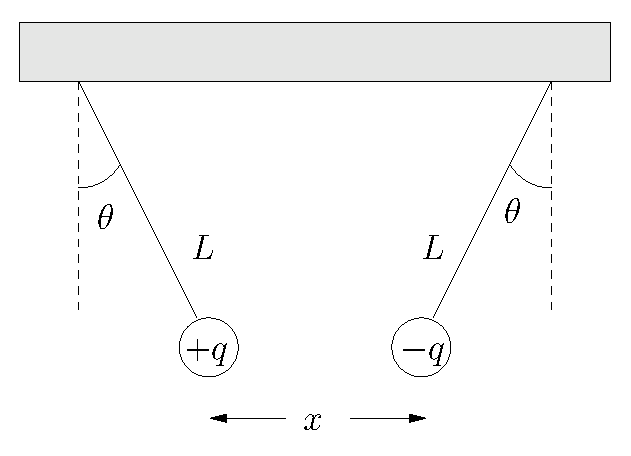
\includegraphics[width=5cm]{additional_problems/ballooncalc}
      \caption{Problem A\ref{prob:balloons}}
    \end{center}
  \end{figure}
\end{aproblem}


\begin{aproblem}{Electric field simulations.}  
  Do Problem 1 on Electric Fields, accessible from the Lecture 1
  calendar page.
\end{aproblem}


\begin{aproblem}{More E-Field Simulations.} 
  Do Problem 2 on Electric Fields, accessible from the Lecture 1
  calendar page.
\end{aproblem}

\begin{aproblem}{Addition of electric fields.} 
  Two charges, each $+5~\mu$C, are on the $y$-axis, one at the origin
  and the other at $y=6\units{m}$.  Find the electric field on the
  $y$-axis at (a) $y=-3\units{m}$, (b) $y = +3\units{m}$, and (c) $y =
  +9\units{m}$.
  \label{prob:addEfields}
\end{aproblem}

\newpage

\begin{aproblem}{Determining $\vec{E}$ using integrals --- semi-infinite rod.} 
  Point {\bf P} is located a distance $a$ from the bottom of a
  semi-infinite rod with uniform linear charge density $\lambda$.
    \begin{enumerate}
    \item Calculate the $x-$component of the electric field at point
      {\bf P}; you should set up and work through the integral.
    \item Calculate the $y-$component of the electric field at point
      {\bf P}; you should set up and work through the integral.
      (Somewhat surprisingly the $x$ and $y$-components have the same
      magnitude.)
    \end{enumerate}
    \label{prob:integ1}

    \begin{figure}[h]
      \begin{center}
        \includegraphics[width=5cm]{additional_problems/integ1}
        \caption{Problem A\ref{prob:integ1}}
      \end{center}
    \end{figure}
\end{aproblem}


\begin{aproblem}{Determining $\vec{E}$ using integrals --- arc.}  
  The figure shows a quarter of a ring with radius $R$ in the $x$-$y$
  plane with a total charge $q$, which is distributed uniformly over
  the quarter-ring. Working through the appropriate integral,
  determine the electric field at the origin (point {\bf P}).
  \label{prob:arc1}

  \begin{figure}[h]
    \begin{center}
      \scalebox{0.7}{\includegraphics{additional_problems/arc1}}
      \caption{Problem A\ref{prob:arc1}}
    \end{center}
  \end{figure}
\end{aproblem}

\newpage

\begin{aproblem}{Computer monitors.} 
  In a computer monitor (the old-fashioned tube-type monitor, not the
  flat panel ones), electrons are fired from the back toward the
  screen.  Assume that the electrons start from rest and are
  accelerated through a potential difference of 50,000 V.
   \begin{enumerate}
   \item What is the energy of the electrons when they hit the screen
     in electron volts?
   \item in Joules?  
   \item What is the speed of impact of the electrons with the screen
     of the monitor?  (You can neglect relativistic effects here,
     although you should note that the speeds aren't {\it that} much
     below the speed of light.)
   \end{enumerate}
   \label{prob:ComputerMonitors}
\end{aproblem}

\begin{aproblem}{Directions of electric fields from continuous sources.}
  The figure shows half of a ring in the $x$-$y$ plane with a varying
  charge density $\lambda$ which depends on the angle $\theta$ from
  the $+x$-axis.
  \begin{enumerate}
  \item Determine the {\bf direction} of the electric field at the
    origin (point {\bf P}) if $\lambda = \lambda_0 \sin{\theta}$.
  \item Determine the {\bf direction} of the electric field at the
    origin (point {\bf P}) if $\lambda = \lambda_0 \cos{\theta}$.
  \end{enumerate}
  \label{prob:arc2}
  \begin{figure}[h]
    \begin{center}
      \includegraphics[width=5cm]{additional_problems/arc2}
      \caption{Problem A\ref{prob:arc2}}
    \end{center}
  \end{figure}
\end{aproblem}

\newpage

\begin{aproblem}{Potential and electric field.} 
  The sketch shows three large parallel plate conductors held at the
  potentials shown. (Assume that the plates are infinitely large.)
  Find the direction and magnitude of the uniform electric field in
  each of the two interior regions. \label{prob:plates}
  \begin{figure}[h]
    \begin{center}
      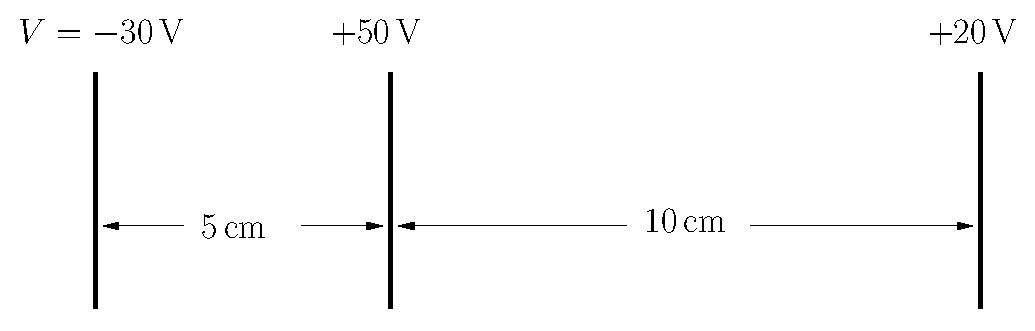
\includegraphics[width=10cm]{additional_problems/plates}
      \caption{Problem A\ref{prob:plates}}
    \end{center}
  \end{figure}
\end{aproblem}


\begin{aproblem}{Resistance and Dimmer Switches.}
  \begin{enumerate}
  \item Make a circuit with two batteries and a light bulb, all in
    series, and note the brightness.  Now add a full length of one of
    your nichrome wires (bare silvery wire) to your circuit between
    the positive side of your batteries and the bulb.  What happens to
    the brightness of the bulb?  Explain briefly.
  \item Repeat with the other equal length piece of nichrome wire.
    Which wire has a larger resistance? % A larger resistivity?
    Explain how you know.  Examine the two wires carefully.  Do you
    note any difference?
  \item Now use just the higher resistance wire in the circuit.
    Carefully unclip the lead on the wire nearest the battery, and
    touch it onto the wire at various places.  How is the bulb's
    brightness affected?  This is basically how a dimmer switch works!
  \end{enumerate}
  \label{prob:dimmer}
\end{aproblem}

\begin{aproblem}{Flashlight circuit}
  Make a circuit with two batteries and two bulbs, all in series.
  \begin{enumerate}
  \item Now replace one of the bulb holders in the circuit with the
    higher resistance nichrome wire, and slide the alligator lead from
    the batteries along the wire (see Prob.~A\ref{prob:dimmer}) until
    the remaining bulb is about as bright as before with the two
    bulbs. This means the resistance of that length of nichrome is the
    same as a bulb. Measure this length.
  \item The wire has a diameter of $0.25\units{mm}$, and the
    resistivity of nichrome is $\rho = 1.0 \times
    10^{-6}\units{$\Omega\cdot$m}$.  Calculate the resistance of the
    length of wire, and therefore of the bulb.  {\bf Continued}$\rightarrow$
  \item From the battery voltage and the resistance that you just
    determined for one bulb, determine the current through the
    original circuit with two bulbs and two batteries.
  \end{enumerate}
\end{aproblem}


\begin{aproblem}{Fun with magnets.}
  Take two cylindrical magnets and let them come together (N of one
  and S of other) around the end of a piece of thread (see
  Fig.~\ref{fig:compass}). You'll end up with what is effectively one
  long magnet (from the two in combination) with a string coming up
  from in between the two (now connected) magnets.  Hold the other end
  of the string and let the magnet dangle.  Now gently twist the
  string from the top. Is there a preferred orientation for the
  magnet? What is this orientation? Explain briefly.
  \label{prob:compass}

  \begin{figure}[h]
    \begin{center}
      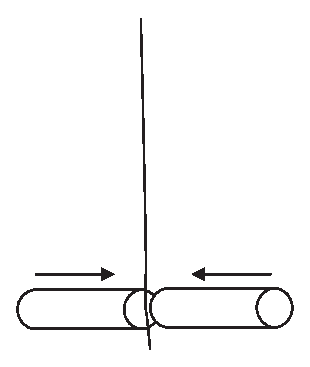
\includegraphics[width=4cm]{additional_problems/compass}
      \caption{Problem A\ref{prob:compass}} \label{fig:compass}
    \end{center}
  \end{figure}
\end{aproblem}


\begin{aproblem}{Mapping the field of a permanent magnet.}
  \begin{enumerate}
  \item Draw a sketch of a cylindrical magnet including the direction
    of the magnetic field in the surrounding region. Mark the
    direction of the magnetic field with little arrows at various
    locations around the magnet.
  \item Now put your cylindrical magnet down on a flat surface and
    keep it from rolling.  Next place your compass in various
    positions around the magnet and draw a sketch of what you observe.
    Your sketch should show a long rectangle (the magnet) surrounded
    by circles (the compass in various locations) with an arrow on
    each circle showing the direction that the red part of the compass
    needle pointed there.  How did your measurements compare to your
    prediction?
  \end{enumerate}
\end{aproblem}

\newpage

\begin{aproblem}{Destroying your TV or computer monitor.}
  (Optional) BE CAREFUL with this one. A strong permanent magnet can
  magnetize parts of your monitor. This causes distortion of the
  images in both shape and color. Most monitors automatically can get
  rid of these extra fields using something called a ``de-gausser'',
  but the de-gausser doesn't usually activate except when the monitor
  is turned on (and is cold), so it might not fix the damage for a
  while, assuming the de-gausser is working.  Thus the caution. Most
  monitors receive no permanent damage, but you never know, so don't
  go wrecking someone else's stuff.

  Bring one of your magnets close to a CRT, like a computer monitor or
  TV. Move the magnet around the front and along the top and
  sides. Write down your observations.  Why does this happen?  What is
  a CRT anyway?
\end{aproblem}


\begin{aproblem}{Magnetic force on a moving particle.}  
  The figure shows a charged particle (with charge
  $-5.0\units{$\mu$C}$) moving with a speed $1.3 \times
  10^5\units{m/s}$ in a vertically-directed magnetic field with
  magnitude $0.8\units{T}$.  The particle is moving at an angle
  $30^{\circ}$ with respect to the horizontal.  Calculate the
  magnitude of the magnetic force on this particle, and state the {\bf
    direction} of the force. \label{prob:magforce}

  \begin{figure}[h]
    \begin{center}
      \scalebox{0.7}{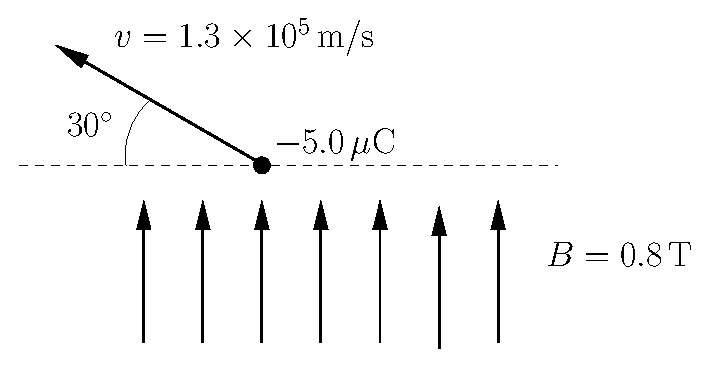
\includegraphics{additional_problems/magforce}}
    \end{center}
    \caption{Problem A\ref{prob:magforce}}
  \end{figure}
\end{aproblem}

\newpage

\begin{aproblem}{Rail guns.}  
  A very simple application of magnetic forces can be used to make a
  nifty device called a ``rail gun.'' These have been proposed as
  devices that could be used to send back to earth (or the moon) raw
  materials mined from an asteroid.  The idea is shown in the figure
  below.  A bar of mass $m$ can slide on two parallel rails separated
  by a distance $H$, and the whole apparatus is in a uniform magnetic
  field with magnitude $B$ pointing into the plane of the paper.  The
  rails are hooked up to a current source, and a current $I$ passes
  through the rails and through the bar, which experiences a force
  that accelerates it down a track of length $D$.  A bucket can be put
  on the bar, and anything in the bucket gets thrown off when the bar
  reaches the end of the rail.

  Given the information above, determine the speed of the bar just
  before it reaches the end of the rails.  (Hint: Think work.)
  \label{prob:railgun}
  \begin{figure}[h]
    \begin{center}
      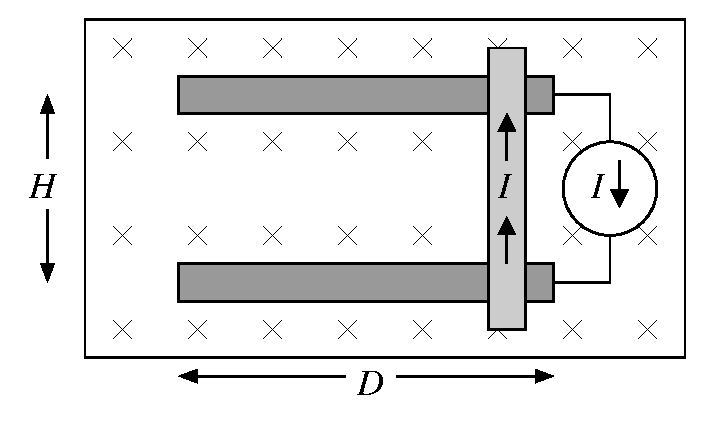
\includegraphics[width=6cm]{additional_problems/railgun}
      \caption{Problem A\ref{prob:railgun}}
    \end{center}
  \end{figure}
\end{aproblem}

\begin{aproblem}{Canceling the Earth's magnetic field.}  
  A 100-turn circular coil with radius $30\units{cm}$ is to produce a
  field at its center that will just cancel the earth's magnetic field
  at the equator, which is $7.0 \times 10^{-5}\units{T}$ directed
  north (horizontal). Find the current in the loop and make a sketch
  that shows the orientation of the loop and the current.
\end{aproblem}


\begin{aproblem}{Why aren't there magnetic fields all around your
house?}
  \begin{enumerate}
  \item The wire to a 100 Watt lamp carries about 1 amp of current to
    light the lamp. Calculate the magnetic field $5\units{mm}$ from a
    wire carrying a steady current of 1 amp.  Compare this to the
    Earth's field of approximately $7 \times 10^{-5}\units{T}$.
  \item Put your compass near various wires in your room leading to
    electrical appliances and lights.  Describe the compass
    deflections.  Why don't you see much?  (Hint: The power cords
    aren't just one wire but are a pair that carry the current both
    {\bf to} and {\bf back from} the appliance/light.)
    \label{prob:PowerCords}
  \end{enumerate}
\end{aproblem}

\begin{aproblem}{An electromagnet.}  
  Take your large and small nail and put them on a table top. Clip one
  end of an alligator lead to a battery (or two in series). Clip
  another to the opposite side of the battery. Wrap the piece of red
  insulated wire many, many times around the larger nail. Hold the
  wrapped nail in one hand and using the other, hook the leads from
  the batteries onto the ends of the wrapped wire to complete the
  circuit.  You're making an electromagnet!

  Try to pick up the small nail with the point of the large nail.
  Once it is off the table, disconnect the leads and see what happens.
  On your paper, explain briefly why the nail becomes a magnet.
\end{aproblem}

\begin{aproblem}{Solenoid.}  
  A solenoid with 2000 turns is $1.3\units{m}$ long, has a radius
  $2.5\units{cm}$ and carries a current of $3.0\units{A}$.  What is
  the approximate magnitude of the magnetic field on the axis near the
  center of the solenoid?
  \label{prob:solenoid}
\end{aproblem}


\begin{aproblem}{Electrical generation.}  
  Commercial electricity generation uses big strong magnets,
  multi-turn coils, and rapid relative motion.  Suppose you could move
  a large $1.0\units{T}$ magnet over the face of a $10\units{cm}$
  diameter 200-turn coil.  What time interval between maximum flux and
  no flux would you need to produce an average emf of $120\units{V}$?
  \label{prob:ElecGen}
\end{aproblem}


\begin{aproblem}{Faraday with derivatives.} 
  A ring with radius $r$ and resistance $R$ lies in the $x$-$y$ plane.
  The ring is located in a spatially uniform, but time-dependent
  magnetic field $\vec{B} = B_0(2-t+3t^2)\, \widehat{k}$.  Calculate
  the magnitude of the electrical current $I(t)$ in the ring as a
  function of time.
  \label{prob:faraday}
\end{aproblem}

\begin{aproblem}{Eddy damping and brakes.} 
  Describe how eddy currents could be used to make brakes for a train
  or a car that don't require any friction.
\end{aproblem}

\begin{aproblem}{The Electromagnetic Spectrum.}  
  Consider the different types of electromagnetic waves: radio waves,
  microwaves, infrared, visible light, ultraviolet light, x-rays and
  gamma rays.  Why do you think there are different names for these
  different kinds of electromagnetic waves?  Is there a meaningful
  distinction?  What are the differences between, say, gamma rays and
  infrared waves?
\end{aproblem}


\begin{aproblem}{Electromagnetic waves and you}.  
  Think about your life, your experiences and things which you may
  {\it not} have experienced but which clearly affect your life. There
  are numerous situations in which electromagnetic waves play a
  significant role in affecting your life.  List {\bf at least} four
  distinct and unique examples.  These list might include things like
  examples of modern technology which rely on electromagnetic waves,
  as well as important electromagnetic wave phenomena which occur in
  the natural world.
\end{aproblem}


\begin{aproblem}{Falling loops.}  
  A long rectangular wire loop with mass $m$ and resistance $R$ is
  falling out of a region with a magnetic field with magnitude $B_0$
  that is pointing out of the plane of the paper.  The rectangle has a
  width $w$ and a length that is so large that part of the loop is
  inside the region with the magnetic field and part is outside that
  region;
  \begin{enumerate}
  \item Determine the current in the wire when the rectangle is
    falling from the magnetic field with a speed $v$.
  \item When dropped from rest the speed of the loop increases from
    $0$ up to the terminal velocity, and then remains constant at this
    terminal velocity.  Determine the terminal velocity for the
    falling loop.  (Assume that the terminal velocity is reached
    before the top of the loop leaves the magnetic field.)
  \end{enumerate}

  \begin{figure}[h]
    \begin{center}
      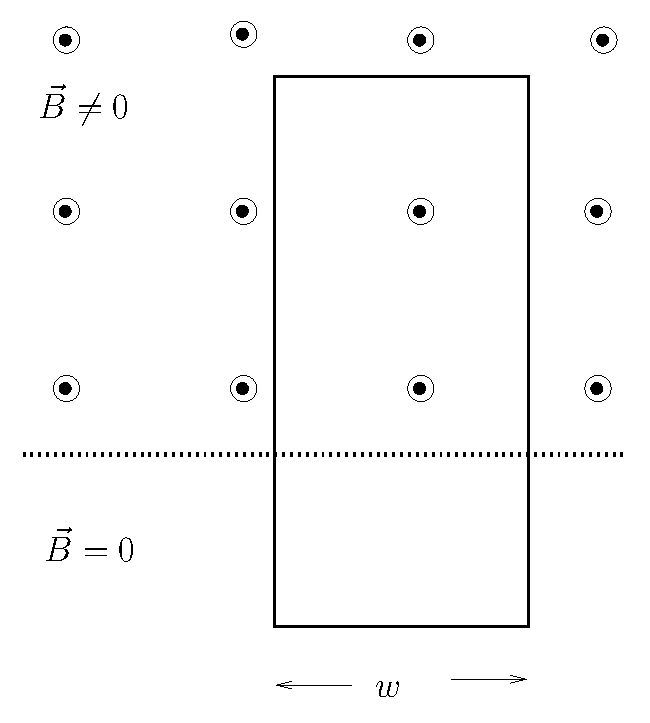
\includegraphics[width=5cm]{additional_problems/bu_em_falling-loop}
      \caption{Problem A\ref{prob:bu_em_falling-loop}}
    \end{center}
  \end{figure}
  \label{prob:bu_em_falling-loop}
\end{aproblem}


\begin{aproblem}{Fetal heartbeat monitors.}  
  The {\it Babycom}$^{\rm TM}$ {\it Home Doppler Fetal Heartbeat
    Monitor} uses ultrasonic waves with frequency $2.5\units{MHz}$,
  and can measure Doppler shifts as low as $100\units{Hz}$.  Calculate
  the approximate speed of the fetal movements (blood flow) that
  account for these $100\units{Hz}$ frequency shifts.  (The speed of
  sound in air is $340\units{m/s}$, and the speed of sound in soft
  tissue --- and water --- is about $1500\units{m/s}$.)
\end{aproblem}


\begin{aproblem}{Electromagnetic waves.} 
  Consider an EM wave with electric field $\vec{E} = (6.6 \times
  10^4\units{N/C})\cos(1.2\pi x - 3.6 \times 10^8 \pi t)\,
  \hat{\jmath}$ with $x$ in meters and $t$ in seconds.  Find the
  expression for the corresponding magnetic field.
\end{aproblem}

\newpage

\begin{aproblem}{Re-radiated Light Waves.}  
  Consider a beam of light propagating along the $y$-axis.  It is
  polarized along the $z$-axis as it enters a diffuse vapor cloud.
  \begin{enumerate}
  \item Along which axis does the electric field of the light wave
    oscillate ($\pm x$, $\pm y$, or $\pm z$)?  How do you know?
  \item Along which axis does the {\it magnetic} field of the light
    wave oscillate ($\pm x$, $\pm y$, or $\pm z$)?  How do you know?
  \item The wave strikes some electrons in the vapor cloud, and they
    start oscillating.  Along which axis do the electrons oscillate
    ($\pm x$, $\pm y$, or $\pm z$)?  How do you know?
  \item These oscillating electrons generate a new re-radiated light
    wave. Along which axis does the electric field of the re-radiated
    wave oscillate ($\pm x$, $\pm y$, or $\pm z$)?  How do you know?
  \item The re-radiated light wave cannot propagate in all directions.
    Along which axis (axes) can the new wave propagate ($\pm x$, $\pm
    y$, or $\pm z$)?
  \item For each answer to part (e), give the axis along which the
    {\it magnetic} field of the re-radiated wave oscillates ($\pm x$,
    $\pm y$, or $\pm z$).
  \end{enumerate}
  \label{prob:reradiation}
\end{aproblem}


\begin{aproblem}{Traveling Waves on a Magic Spring.} 
  Take your Magic Spring and attach one end to a door knob, bed post
  or a friend.  Hold the other end and walk away so the spring is
  stretched to about 6 feet.  Grab a few of the coils and pull them
  toward you and release so that a longitudinal compression wave
  travels along the spring, bounces off the other end, and goes back
  and forth.  See how far the pulse goes in five seconds (\# of round
  trips times round-trip distance) and estimate the wave speed.
  Repeat by pulling the coils sideways to get a transverse wave, and
  find its wave speed.  Are they different?  Compare to the speeds
  found in Question A\ref{a:standingwave}. \label{a:travwave}
\end{aproblem}


\begin{aproblem}{Standing Waves on a Magic Spring.}  
  Find a friend to help you time and count Magic Spring standing wave
  oscillations.
  \begin{enumerate}
  \item Hold the spring with one end in each hand and generate
    standing waves as demonstrated in lecture.  Get at least the
    fundamental and the next two higher harmonics.  (Prize if you can
    demonstrate the $n=5$ mode or higher!)  Notice how the frequency
    you need to use changes for as the mode number increases.
  \item For quantitative analysis, set up the spring just as you had
    it when you measured pulse speeds in Question A\ref{a:travwave}.
    Set up the lowest frequency standing wave by shaking one end of
    the spring and count ten full oscillations while your friend
    measures the time for these ten oscillations.  Determine the
    period, frequency, and wavelength for this mode.  Repeat your
    measurements for the $n=2$ and $n=3$ modes, making sure that you
    keep the length of the spring (the distance between your ``shaking
    hand'' and the fixed end) approximately the same for all of your
    measurements.
  \item What is the ratio of the frequency of the $n = 2$ mode to the
    fundamental frequency?  What is the ratio of the frequency of $n =
    3$ mode to the fundamental?  Is this what you expect?
  \item Use the wavelength and corresponding frequency for each mode
    to determine a wave speed.  Compare these to the speed of
    transverse waves measured in Question A\ref{a:travwave}.
  \end{enumerate}
  \label{a:standingwave}
\end{aproblem}


\begin{aproblem}{A musical octave.}  
  Use your slide whistle for this one.
  \begin{enumerate}
  \item Extend the slide all the way out.  Blow softly on the whistle
    and note the pitch.  Now push the slide in as you continue to
    blow.  What do you hear?  Explain {\it why} you hear the changes
    in the pitch that you hear when the slide is pushed inward.
  \item Extend the slide all the way out again.  Again, blow softly on
    the whistle and note the pitch.  Now continue to play the whistle
    as you push the slide inward, and stop when you reach a note that
    is an octave above what you started with. (This may take many
    tries to match.)  What determines how far the slide should be
    pushed in to increase the pitch by one octave?  Try to see if you
    can make a simple (approximate) measurement to verify your theory.
  \end{enumerate}
\end{aproblem}


\begin{aproblem}{Annoying your roommate.} 
  Here is another opportunity to play with your slide whistle.
  \begin{enumerate}
  \item Play the slide whistle softly with the slide mostly or all the
    way out.  Make a sketch of the standing wave in the air column
    associated with this note.
  \item Now blow harder on the slide whistle until the pitch changes.
    How is the frequency of this new (and most assuredly
    less-pleasant-sounding) note related to the one from part (a)?
    Draw a sketch of the standing wave to support your answer.
  \item Now plug your ears and blow even harder.  You should be able
    to get the pitch to jump again (and to attract any stray dogs that
    are in the neighborhood, along with a few irate hall-mates). How
    is the frequency of {\it this} note related to the one from part
    (a)?  Draw a sketch of the standing wave to support your answer.
  \end{enumerate}
\end{aproblem}

\newpage

\begin{aproblem}{Organ pipes.}  
  Consider a $10\units{m}$ organ pipe, open at both ends.
  \begin{enumerate}
  \item Sketch the standing wave pattern for the three longest
    wavelength modes.
  \item From each sketch, determine the wavenumber $k$ and the
    wavelength $\lambda$.
  \item Given your answers for (a) and (b), and given the speed of
    sound in air ($340\units{m/s}$), determine the frequency of each
    mode.
  \end{enumerate}
  \label{prob:OrganPipes}
\end{aproblem}


\begin{aproblem}{Stringed instruments.} 
  The lowest note that can be played on a bass fiddle is E1 (frequency
  41.2 Hz) on a string of length $1.2\units{m}$ (secured at both
  ends).
  \begin{enumerate}
  \item Sketch the standing wave pattern for the three longest
    wavelength modes.
  \item From each sketch, determine the wavenumber $k$ and the
    wavelength $\lambda$.
  \item Determine the wave speed for this string.
  \end{enumerate}
\end{aproblem}

\begin{aproblem}{Beats.}  
  Find someone else who is taking PHYS 212. One of you should blow
  (softly) your slide whistle with the slide somewhere in the
  middle. Hold the note while the other person blows his/her whistle
  and slowly adjusts his/her slide around the position of your slide.
  Listen for the beats and comment on how they change as the frequency
  of the second whistle is varied.
\end{aproblem}


\begin{aproblem}{Polarized light.}  
  Take your polarized disks and look at the following things and
  comment on what you observe:
  \begin{enumerate}
  \item Go outside on a sunny day when the sun is low in the sky,
    preferably early or late in the day and look straight up at the
    sky, looking through one of the Polaroid disks.  Then turn the
    disk.  What do you observe?  What does this tell you about light
    scattered from the sky?
  \item Look at various different LCDs (liquid-crystal displays): your
    calculator, a laptop or flat-screen monitor, a gas station pump
    readout, etc.  Rotate the Polaroid disk and comment on what you
    observe.  What does this tell you about liquid-crystal displays?
  \item How could you determine definitively if some sunglasses that
    you were buying at Wal-Mart$^{TM}$ were polarized?  (Don't trust
    the labels: my wife once bought ``polarized'' sunglasses that
    turned out to be fakes.)
  \end{enumerate}
\end{aproblem}

\newpage

\begin{aproblem}{Soap films and bubbles.} 
  \begin{enumerate} 
  \item Here's one to try in the shower! Get your hands very wet and
    soapy. Then slowly slide your forefinger along your thumb
    stretching a soap film bigger and bigger.  You can catch it on
    your other hand as demoed in lecture to make a big thin film.  In
    fact, if your hands are wet, you can catch soap bubbles without
    popping them. (This is a great thing to do on a day just after it
    has rained --- blow a bunch of soap bubbles on the wet pavement.
    They won't pop.)

    If you are not good at this, try using bubbles from the soap
    bubble bottle in your kit.  Blow a big bubble, catch it on the
    wand, and hold it while it thins out.

    Now with the light behind you, look at the reflections off the
    film. You should see some really cool patterns of colors!  Try to
    sketch the patterns (later) and show where each color is.  In a
    few sentences, try to explain what you see in terms of thin films
    that you studied in class.

  \item (Optional if weather cooperates.)  After it has rained, look
    at the pavement in the street or parking lots where cars are or
    have been.  You might see a blotch of color.  This usually
    indicates that a drop of oil has fallen on the ground.  (A good
    place to look for these splotches is underneath cars driven by
    Bucknell faculty.) If you see one of these colorful oil spots, try
    stepping on it or brushing your foot over it.  Comment on what you
    see and try to explain what you see in terms of the thin films
    that you studied in class.
  \end{enumerate}
\end{aproblem}


\begin{aproblem}{Fiber optics toy.} 
  Load up your fiber optics flashlight toy (Galaxy Wand) with the two
  little batteries (this may have already been done for you). Turn it
  on and notice how the cool colors of light come out the ends of the
  fibers but not out the sides.  Take one of the fibers and bend it
  until it kinks. (If it breaks, try again.)  Some of the light in
  that fiber will escape.  Why does it escape?  Why doesn't it escape
  if you make smooth curves in the fiber rather than a kink?
\end{aproblem}


\begin{aproblem}{Thin film interference.} 
  Assume that light with a wavelength $\lambda_0$ in air falls on a
  thin film composed mostly of water (index of refraction $n_w$) and
  with a thickness $t$.  Assume that the water is on top of a mirror
  which inverts the EM wave when it reflects it.
  \begin{enumerate}
  \item What is the wavelength of the light inside the film (in terms
    of $\lambda_0$ and $n_w$)?
  \item What is the path length difference between the light reflected
    off the front of the film and that which goes through the film,
    reflects off the mirror, and {\it then} comes back through the
    film and out the front?
  \item Are either (or both) of the two beams of reflected light
    inverted due to the reflection?
  \item What is the phase difference between the two reflected beams?
    (Hint: use the wavelength of the light {\it inside} the water
    film.
  \item If $n_w = 1.33$ and the film has a thickness $t =
    300\units{nm}$, what is the largest wavelength of light (when in
    air) for completely destructive interference?  For completely
    constructive interference?
  \end{enumerate}
\end{aproblem}


\begin{aproblem}{Son of thin film interference.} 
  Assume that light with a wavelength $\lambda_0$ falls on a thin film
  composed mostly of water (index of refraction $n_w$) and with a
  thickness $t$. Assume that the film is surrounded by air on both
  sides.

  If $n_w = 1.33$ and the film has a thickness $t = 300\units{nm}$,
  what is the longest wavelength of light (when in air) for completely
  destructive interference in the reflected light?  For completely
  constructive interference?
\end{aproblem}


\begin{aproblem}{Interference in music.}  
  Sitting at your desk, you are listening to music from your stereo.
  Your right ear is $2.2\units{m}$ from one speaker and $2.6\units{m}$
  from the other.  Nostalgic for your formative childhood years, you
  are listening to a {\it Barney's Greatest Hits} CD, and there is a
  particular solo by Barney in which the frequency of his tune ranges
  up to $1800\units{Hz}$.  Ignoring reflections, determine the two
  smallest frequencies at which there will be destructive interference
  of the sound at your right ear; i.e., where the sound will be
  weakest.
\end{aproblem}


\begin{aproblem}{DVDs.}  
  If you shine laser light with wavelength $650\units{nm}$ at normal
  incidence onto the surface of DVD, you'll find first-order intensity
  maxima coming back from the surface at an angle about $65^{\circ}$
  from the normal.  Use this information to estimate (a) the spacing
  between adjacent grooves on a DVD (we know, it's one big spiral, but
  we want the spacing between the adjacent loops in the spiral); and
  (b) the approximate number of grooves (or loops of the spiral) on
  the disk, assuming a radius of approximately $4\units{cm}$ for the
  disk.
  \label{prob:dvds}
\end{aproblem}


\begin{aproblem}{Compact disks.} 
  Take a copy of your favorite CD (or your least favorite one -- it
  doesn't matter) and look at the groovy side in strong light. Tip the
  CD at different angles. Why do you see colors?  Do they change for
  different tip angles? Explain briefly.
\end{aproblem}

\newpage

\begin{aproblem}{Resolution.} 
  Go out to the Academic Quad at the end opposite the library. Looking
  at the clock on the library tower, walk toward the library until you
  can just distinguish the five separate lines that make up the Roman
  numeral 8 (VIII).  Now pace off your distance to the library doors.
  Add $30\units{ft}$ to get the distance between your former position
  and the clock face.  (Assume that each pace is about
  $75\units{cm}$.)

  Now using Rayleigh's criterion, calculate the minimum separation of
  objects on the clock face that you could distinguish with the naked
  eye.  Assume that the visible light you use has a wavelength of
  $500\units{nm}$.  How does your calculated separation compare with
  Prof.  Bowen's estimate of the actual separation between lines
  ($5\units{cm}$)?
\end{aproblem}


\begin{aproblem}{Complex traveling wave.} 
  The electric field of a traveling wave is represented by
  \[
  \vec E(x,t) = 6\times 10^4\, e^{i(0.5\times 10^7 x - 1.5\times
    10^{15}t)}\,\hat k
  \]
  with $E$ in N/C, $x$ in meters, and $t$ in seconds.
  \begin{enumerate}
  \item Calculate the wavelength, period, and wave speed of this wave.
    What kind of EM wave is this?
  \item Determine the amplitude of the associated magnetic field wave
    (in Tesla).
  \item Determine the direction of propagation for this wave.
  \item Using the gnuplot graphing program, plot the real part of
    $E_z$ at both $t=0$ and $t=10^{-15}\units{s}$.  Did the wave move
    visibly in this short time?
  \end{enumerate}
  \label{prob:complex_traveling_wave}
\end{aproblem}


\begin{aproblem}{Wave nature of light.}  
  Here's an easy way to see a manifestation of the wave nature of
  visible light.  Put on your diffraction glasses and look at a small
  bright light source.  Sketch the pattern in your notes.  Explain
  briefly why this pattern is indicative of the light's wave
  properties.
\end{aproblem}

\addtocounter{prob}{3}

\begin{aproblem}{Implications of photoelectric effect.} 
  Professor Quack doesn't believe in quantum theory.  To make his
  point he does a photoelectric experiment.  He takes a white light
  source and two filters --- one filter allows blue light to pass, and
  one filter allows green light to pass.  He measures the current when
  the blue filter is in place and finds that it is {\em less} than the
  current he measures with the green filter in place.  He argues that
  according to quantum theory blue photons should have more energy
  than green photons, so the blue light should result in a greater
  current than that caused by the green light.  What do you have to
  say to Professor Quack?
\end{aproblem}


\addtocounter{prob}{4}

\begin{aproblem}{Proton in a box.} 
  A proton is confined to a one-dimensional infinite potential well
  with a width of $2 \times 10^{-14}$ m.  Assume that it is in its
  first excited state (i.e., not the ground state, but the next
  state).
  \begin{enumerate}
  \item Draw a sketch of the wavefunction $\psi$ corresponding to this
    state, and indicate the locations where you would never expect to
    find the proton.
  \item Determine the wavelength of the quantum wave associated with
    the proton.
  \item Using your answer to part (b), determine the magnitudes of the
    momentum and energy of the proton in the first excited state.
  \end{enumerate}
  \label{prob:proton_in_box}
\end{aproblem}


\begin{aproblem}{Electron in a box.}  
  An electron is confined to a one-dimensional infinite potential well
  of width $b$, and is in its second excited state.  The energy of the
  electron is $75\units{eV}$.  (Remember that the energy is all
  kinetic in this case.)
  \begin{enumerate}
  \item Calculate the momentum of the electron.
  \item Use your result from part (a) to calculate the wavelength of
    the electron.
  \item Draw a sketch of the wavefunction $\psi$ corresponding to this
    state, and indicate the locations where you would never expect to
    find the electron.
  \item Use your answers from parts (b) and (c) to calculate the width
    of the potential well $b$.
  \end{enumerate}
\end{aproblem}


\begin{aproblem}{Whirl-a-Tune and quantization.} 
  Take your ``whirl-a-tune'' tube and hold the end with the little
  neck.  Then whirl the tube slowly over your head and listen for a
  tone.  Whirl faster and slower and note the pitch that you hear.
  Can you get any frequency or just certain discrete tones?  Explain
  briefly why only certain frequencies are heard.  The
  ``quantization'' of frequencies that you hear in this case involves
  the same sort of wave mechanics as the quantization of energy levels
  in a (small) confined system.
\end{aproblem}

\newpage

\begin{aproblem}{Uncertainty.}  
  A wide beam of particles with mass $m$ and horizontal momentum
  $\vec{p}_1$ is sent toward a vertical slit of width $a$.  Consider
  one particle that you know makes it through the slit, but you know
  absolutely nothing else about the particle.
  \begin{figure}[h]
    \begin{center}
      \scalebox{0.4}{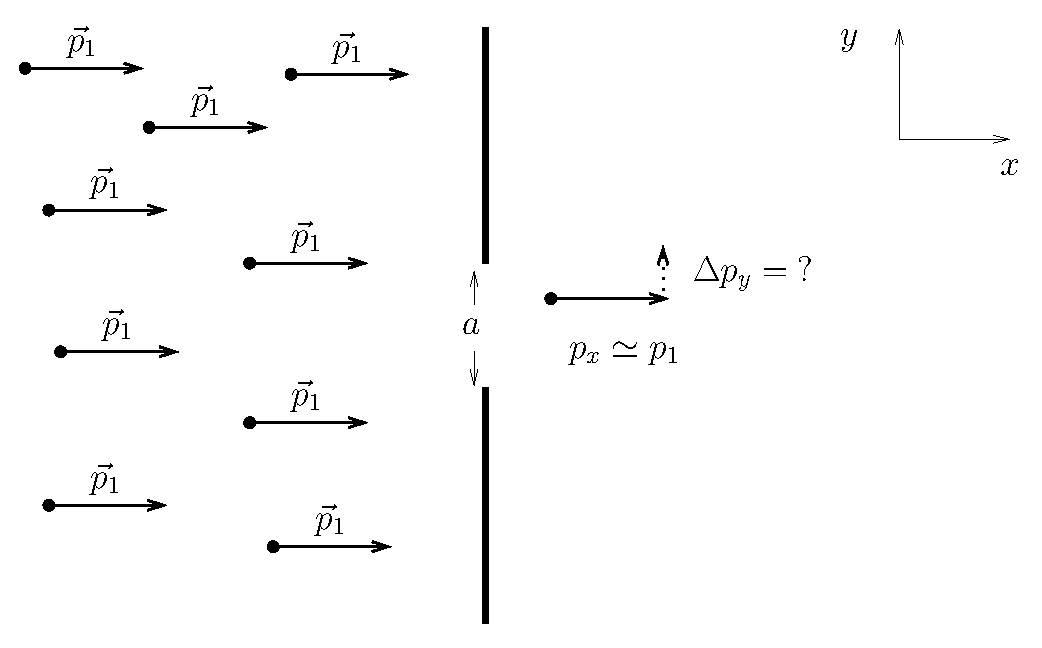
\includegraphics{additional_problems/uncertainty}}
      \caption{Problem A\ref{prob:uncertainty}}
    \end{center}
  \end{figure}
  \begin{enumerate}
  \item What is the approximate uncertainty in the vertical position
    of the particle right after it passes through the slit? (Don't
    make this harder than it is; the answer should be obvious.)
  \item Determine the approximate minimum uncertainty in the vertical
    momentum of the particle right after it passes through the slit.
    
    \begin{figure}[h]
      \begin{center}
        \scalebox{0.35}{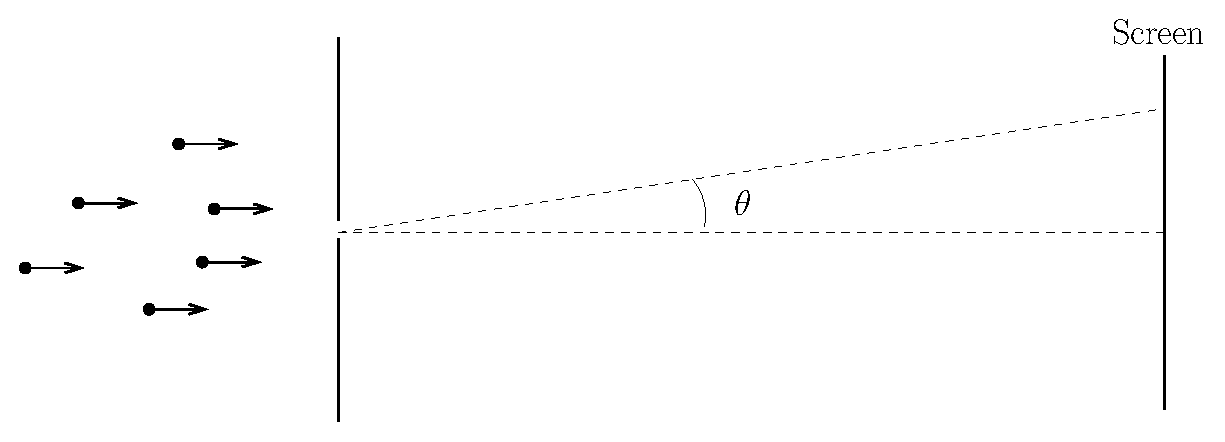
\includegraphics{additional_problems/uncertainty2}}
        \caption{Problem A\ref{prob:uncertainty}}
      \end{center}
    \end{figure}
  \item If the particle is detected on a faraway screen, show that you
    expect to find particles hit the screen over a range of angles
    $\pm \theta$, where $\theta \simeq \tan^{-1}[\lambda/(2\pi a)]$.
  \end{enumerate}
  \label{prob:uncertainty} 
\end{aproblem}


\begin{aproblem}{More uncertainty.}  
  The position of a macroscopic particle of mass $0.04\units{kg}$ is
  measured to an accuracy of $\approx 10^{-12}\units{m}$.  (This can
  actually be done using interferometers.)  Compute the minimum
  uncertainty in the velocity of the object.
  \label{prob:moreuncertainty} 
\end{aproblem}

\newpage

\begin{aproblem}{Magic Springs and the Particle-in-a-Box.}  
  Hold both ends of your Magic Spring, and get standing waves in the
  first, second, and third lowest frequency modes.  Sketch the wave
  patterns and compare them to the wave functions for the three lowest
  energy states of a ``particle in a box.''
\end{aproblem}

\begin{aproblem}{Schr\"{o}dinger equation for a classically allowed
situation.}  
  Consider a particle of mass $m$ in a region in which the potential
  energy is constant, i.e., $U(x)=U_0$, and assume that the total
  energy of the particle $E$ is greater than the potential energy,
  i.e., $E>U_0$.  (This is the case for classically allowed motion.)
  To determine the wave function we must find a function $\psi(x)$
  that satisfies the one-dimensional Schr\"{o}dinger equation
  \[ -\frac{\hbar^2}{2m} \frac{d^2\psi(x)}{dx^2} + U(x)\psi(x) 
  = E\psi(x).  
  \]
  In this problem you will try three ``guesses'' for $\psi(x)$ and see
  if they satisfy the Schr\"{o}dinger equation. The three ``guesses''
  are
  \begin{itemize}
  \item $\psi_1(x) = Ax^2$ 
  \item $\psi_2(x) = B\sin(kx)$
  \item $\psi_3(x) = Ce^{-\kappa x}$,
  \end{itemize}
  where $A$, $B$, $C$, $k$, and $\kappa$ are undetermined real
  constants.
  \begin{enumerate}
  \item Rearrange the Schr\"{o}dinger equation so that the second
    derivative $d^2\psi/dx^2$ is alone on the left.
  \item Plug $\psi_1(x)$ into the Schr\"{o}dinger equation and see if
    there is any choice for the constant $A$ that will make
    $\psi_1(x)$ satisfy the equation for all values of $x$.
  \item Plug $\psi_2(x)$ into the Schr\"{o}dinger equation and see if
    there is any choice for the constants $B$ and $k$ that will make
    $\psi_2(x)$ satisfy the equation for all values of $x$ .
  \item Plug $\psi_3(x)$ into the Schr\"{o}dinger equation and see if
    there is any choice for the constants $C$ and $\kappa$ that will
    make $\psi_3(x)$ satisfy the equation for all values of $x$.
  \item You should have found that $\psi_2(x)$ can be a solution for
    the proper choice of $k$.  Determine the wavelength of the
    oscillations in terms of $\hbar$, $m$, $E$, and $U_0$. (i.e.,
    solve for $k$ and remember from the waves unit that
    $k=2\pi/\lambda$.)  Is your result consistent with that predicted
    from the de~Broglie relationship?  (Hint: $E-U_0$ is the kinetic
    energy $K = p^2/2m$.  Re-write things in terms of the momentum and
    the answer should drop into your lap.)
  \end{enumerate}
\end{aproblem}


\begin{aproblem}{Schr\"{o}dinger equation for classically forbidden
situation.}  
  Consider a particle of mass $m$ in a region with a constant
  potential energy $U_0$, and assume that the total energy of the
  particle $E$ is {\em less} than the potential energy, i.e., $E<U_0$.
  (This isn't possible for classical motion, but continue anyway.)  To
  determine the wave function we must find a function $\psi(x)$ that
  satisfies the one-dimensional Schr\"{o}dinger equation
  \[ -\frac{\hbar^2}{2m} \frac{d^2\psi(x)}{dx^2} + U(x)\psi(x) 
  = E\psi(x).  
  \]
  In this problem you will try three ``guesses'' for $\psi(x)$ and see
  if they satisfy the Schr\"{o}dinger equation. The three ``guesses''
  are
  \begin{itemize}
  \item $\psi_1(x) = Ax^2$ 
  \item $\psi_2(x) = B\sin(kx)$
  \item and $\psi_3(x) = Ce^{-\kappa x}$,
  \end{itemize}
  where $A$, $B$, $C$, $k$, and $\kappa$ are undetermined real
  constants.
  \begin{enumerate}
  \item Rearrange the Schr\"{o}dinger equation so that the second
    derivative $d^2\psi/dx^2$ is alone on the left.
  \item Plug $\psi_1(x)$ into the Schr\"{o}dinger equation and see if
    there is any choice for the constant $A$ that will make
    $\psi_1(x)$ satisfy the equation for all values of $x$.
  \item Plug $\psi_2(x)$ into the Schr\"{o}dinger equation and see if
    there is any choice for the constants $B$ and $k$ that will make
    $\psi_2(x)$ satisfy the equation for all values of $x$.
  \item Plug $\psi_3(x)$ into the Schr\"{o}dinger equation and see if
    there is any choice for the constants $C$ and $\kappa$ that will
    make $\psi_3(x)$ satisfy the equation for all values of $x$.
  \end{enumerate} 
\end{aproblem}

\begin{aproblem}{Tunneling and time-energy uncertainty.}  
  Consider an electron hitting a barrier.  Assume the electron has an
  energy $E = 50\units{eV}$, and the barrier has a height $U =
  100\units{eV}$.  Semi-classically, to tunnel through the barrier,
  the electron must ``borrow'' enough energy to get over the barrier,
  and must hold this energy long enough to travel the width of the
  barrier.  The best-case scenario is if the energy fluctuates up to a
  value of $2U - E$ or $150\units{eV}$.  (See ``Optional problem''
  below if you want to see where this comes
  from.) \label{prob:tunneltime}

  \begin{enumerate}
  \item Using the energy-time uncertainty relation $\Delta E \Delta t
    \approx \hbar$, approximate the typical duration of the energy
    fluctuation (i.e., determine $\Delta t$).
  \item Determine the classical velocity of the electron in the
    barrier region if it has an energy of $150\units{eV}$.  (Warning:
    the kinetic energy of the electron is not $150\units{eV}$ here.)
  \item Determine the maximum width $L$ of the barrier such that the
    electron will make it through in a time $\Delta t$.
  \item The width $L$ that you have just determined is a width for
    which you would expect a reasonable probability for an electron to
    tunnel through a barrier.  You can calculate the transmission
    probability $T$ explicitly by $T = e^{-2\alpha L}$, where $\alpha
    = \sqrt{2m(U-E)/\hbar^2}$.  Use your value of $L$ and the
    information given above to verify that you get a reasonable value
    for $T$. (by ``reasonable,'' we mean that you should get a
    probability greater than 0.1, but, of course, it must be less than
    1.)
  \end{enumerate}
\end{aproblem}


\begin{aproblem}{Optional for mathophiles \dots} 
  (You don't have to hand this in.)  For the preceding ``A'' problem,
  show that the semi-classical approach discussed for tunneling gives
  the largest value of the barrier width $L$ if the particle borrows
  enough energy $\Delta E$ to get to an energy of $(2U - E)$. Hint:
  Use the approach from the previous problem to find the maximum
  barrier width $L$ if the particle fluctuates up to an energy of
  $E_{\rm high}$.  Then take the derivative $dL/dE_{\rm high}$ and set
  this equal to zero to figure out the optimal $E_{\rm high}$.  Note:
  conceptually, the optimal energy is a small enough energy such that
  $\Delta t$ is relatively long, but large enough such that the
  electron still has some kinetic energy while traveling across the
  barrier.
\end{aproblem}


\begin{aproblem}{Semi-infinite square-well potential.} 
  Download the Excel worksheet \verb+semi-finite.xls+ from either the
  {\it Handouts} page or from the Calendar page.  This sheet shows the
  calculations for determining the wavefunctions for a potential well
  that is infinite at $x=0$ but of finite magnitude on the right side
  of the well (which is at $x=5$ in this problem).  You'll see two
  graphs: the top one shows the semi-infinite potential well (in
  purple) along with a non-normalized plot of the calculated
  wavefunction so you can see it along with the potential.  The bottom
  graph shows the normalized wavefunction, corresponding to the
  second-to-last column in the worksheet.

  When you bring up the worksheet, the energy will be set for the
  value for the ground state.  Some questions:

  \begin{enumerate}

  \item Sketch or print out (just the first page!) the wavefunctions
    that are displayed for the ground state along with at least two of
    the excited states.  To display the 1$^{\rm st}$ and $2^{\rm nd}$
    excited states, type in 0.64282 and 1.4144 respectively in the
    framed box for energy.

  \item What happens if you type in an energy that {\bf isn't} one of
    the well-defined energies for the problem?  Try it out, and
    comment on what happens.  Had we not told you what the allowed
    energies were, how might you figure them out?  (You'll be doing
    this in lab later this semester.)  {\bf Continued} $\rightarrow$

  \item For any of the allowed states, show that the state plotted in
    the bottom graph is normalized.  Hint: we have already created a
    column for the square of the normalized wavefunction (the
    right-most column).  You might want to take advantage of the
    \verb+sum(start:end)+ routine in Excel.

  \end{enumerate}
\end{aproblem}

\begin{aproblem}{Classically allowed and classically forbid\-den
probabilities.}  
  Load the \verb+semi-finite.xls+ worksheet (the same one from the
  previous problem).  The ground state should be displayed initially.
  \begin{enumerate}
  \item If a measurement were done on this system, what would be the
    probability that the particle would be found in the region $x <
    5$?  Explain briefly how you calculated this from the Excel
    worksheet. \\ {\bf Hint:} Remember that for a continuous
    wavefunction $\psi(x)$, the probability of finding the particle in
    a particular region is\\ $\int_{x_1}^{x_2} P(x)\, dx = \int |\psi
    (x)|^2\, dx$.  However, we don't actually have a wave function to
    integrate; we have a numerical solution instead.  But we can do a
    {\it Riemann Sum} and add up the contributions: $\sum_i P(x_i)\,
    \Delta x = \sum |\psi(x_i)|^2\, \Delta x$. You'll have to
    determine what $\Delta x$ is in this Excel worksheet.
  \item What would be the probability that the particle would be found
    in the region $x > 5$?
  \item What would be the answer to questions (a) and (b) if this was
    a classical particle in a semi-infinite square-well potential with
    energy less than $U_0$ (i.e., no quantum effects)?
  \item Answer questions (a) and (b) again, but for the second excited
    state (with $E = 1.4144$).  Compare your answers with those for
    the ground state.  Do the results make sense, considering the
    higher energy? Explain.
  \item What do you think would happen if the potential dropped back
    to 0 at $x=6$?  Would the particle remain trapped indefinitely?
    Explain why or why not, and refer to the graphs to support your
    answer.  (You might want to sketch them or print them out.)
  \end{enumerate}
\end{aproblem}

\newpage

\begin{aproblem}{Wavefunctions and potential energy.} 
  The illustrated graph gives the wavefunction for bound state of an
  electron in some one-dimensional potential well.

  \begin{figure}[h]
    \begin{center}
      \scalebox{0.6}{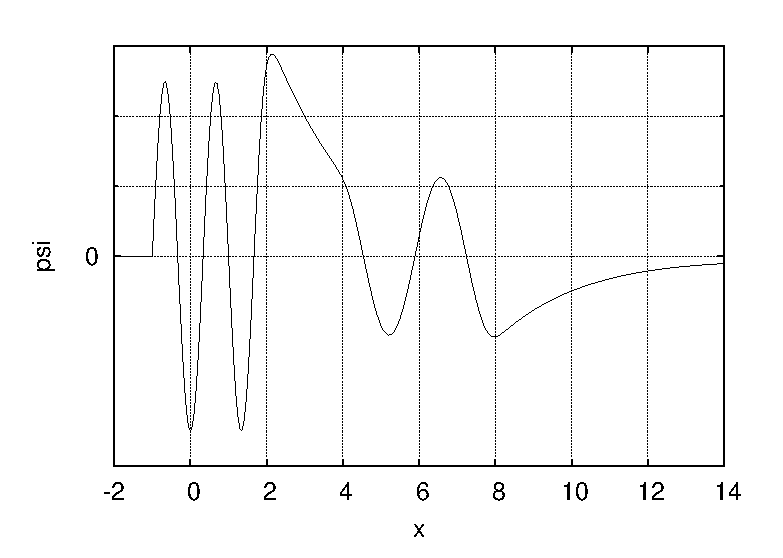
\includegraphics{additional_problems/wavefunction}}
      \caption{Problem A\ref{prob:psi-u}}
    \end{center}
  \end{figure}

  Make a qualitative sketch of the potential energy $U(x)$ versus $x$
  that could give rise to this wavefunction.  Include an indication of
  the total energy $E$ on your sketch.
  \label{prob:psi-u}
\end{aproblem}
    

\begin{aproblem}{Wavefunctions and probabilities.} 
  Using the sketch below, of the wavefunction $\psi (x)$, identify
  which letters indicate locations where the particle is: (a) most
  likely to be found and (b) least likely to be
  found. \label{prob:wavefn}

  \begin{figure}[h]
    \begin{center}
      \scalebox{0.5}[0.75]{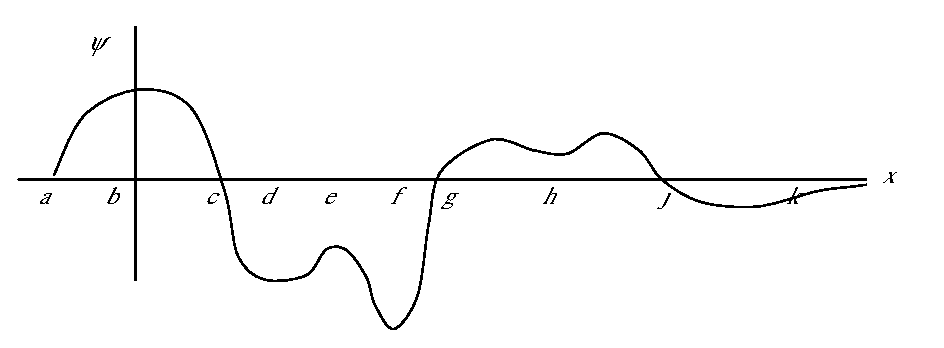
\includegraphics{additional_problems/wavefunction2}}
      \caption{Problem A\ref{prob:wavefn}}
    \end{center}
  \end{figure}
\end{aproblem}


\begin{aproblem}{Barrier tunneling:  Calculating approximate
probabilities.}  
  A $15\units{eV}$ electron is incident on a potential barrier of
  height $22\units{eV}$ and width of $0.05\units{nm}$.

  \begin{enumerate}
  \item Use the transmission probability discussed in part (d) of
    Problem A\ref{prob:tunneltime} to estimate the order of magnitude
    of the probability that the electron will tunnel through the
    barrier.
  \item If one million electrons with energy $15\units{eV}$ hit this
    barrier, roughly how many of them would you expect to get through?
  \item Repeat parts (a) and (b) for a barrier width of
    $0.5\units{nm}$.
  \end{enumerate}
\end{aproblem}


\begin{aproblem}{Annoying your roommate, Part 2} or {\bf Superposition
of states.} 
  Take your slide whistle and with the slide most or all the way out,
  blow gently into the whistle.  As we discussed in the previous unit,
  the note that you hear is due to the fundamental mode of the slide
  whistle.  If you blow harder, the pitch will jump to a higher value,
  corresponding to the second standing-wave mode.

  It is possible to blow hard enough -- but not too hard -- such that
  you hear two notes at the same time.  Do this, and comment on what
  you hear.  Now, consider the analogous quantum problem.  If these
  were two matter waves instead of sound waves, what would the
  different pitches that you hear correspond to?
\end{aproblem}


\begin{aproblem}{Life in a quantum world.} 
  Last semester we asked you to describe some relativistic effects
  that you would notice if the physical ``speed limit'' of light were
  $4\units{mph}$ instead of $3 \times 10^8\units{m/s}$. Now imagine
  that the quantum constant $\hbar$ were 1 Joule-sec.
  \begin{enumerate}
  \item The uncertainty principle in this world would be $\sigma_x
    \sigma_p \geq \frac{1}{2}\units{kg$\cdot$m$^2$/s}$.  Imagine that
    someone throws a ball to you. Describe what you would experience
    trying to catch the ball.
  \item Consider the energy of a photon.  With light frequencies still
    in the $10^{14}\units{Hz}$ range, describe how it would feel to be
    sunbathing on a beach.
  \item What would your approximate de~Broglie wavelength be when
    walking? What would happen when you walk through a doorway?
  \end{enumerate}
\end{aproblem}

\newpage

\begin{aproblem}{Transitions.}  
  The sketches below show the state of a two-level atom and possibly a
  photon.  For each ``Before'' sketch make a corresponding ``After''
  sketch and name the process.
  \label{prob:transition}

  \begin{figure}[h]
    \begin{center}
      \scalebox{0.5}{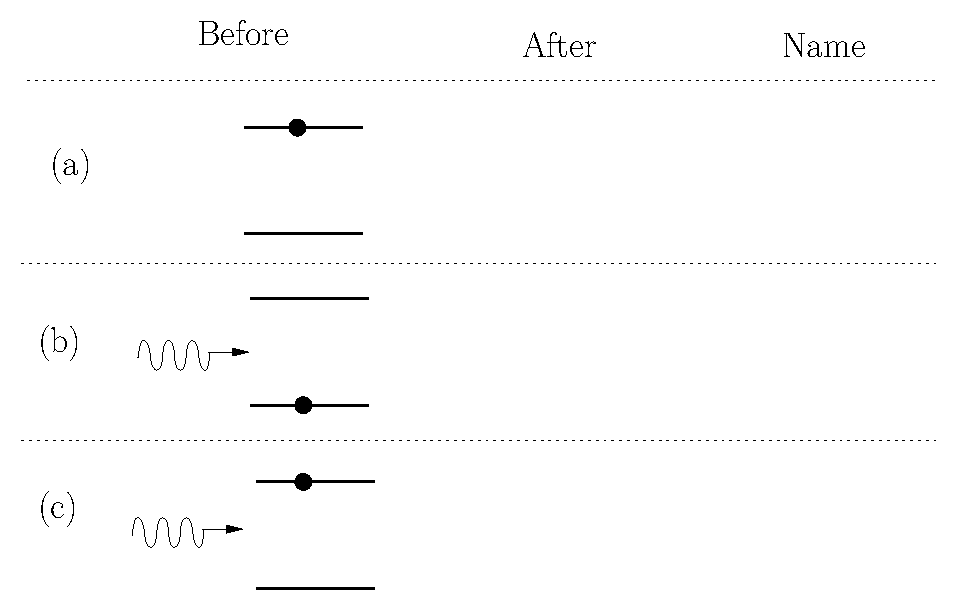
\includegraphics{additional_problems/transitions}}
      \caption{Problem A\ref{prob:transition}}
    \end{center}
  \end{figure}
\end{aproblem}


\begin{aproblem}{Population inversion.} 
  Explain briefly why a population inversion is necessary for the
  operation of a laser.
\end{aproblem}


\begin{aproblem}{Superconductors.} 
  (Do in Problem Session) Here we investigate some magnetic properties
  of superconductors.
  \begin{enumerate} 
  \item Closely observe the little cube hovering over the
    disk. Comment on what you observe.  What evidence do you have that
    this is a superconductor?  Can you make the cube spin?
  \item Explain how the superconductor can levitate the magnet.
  \end{enumerate}
\end{aproblem}


\begin{aproblem}{Flipping magnets.} 
  Find a friend to help you explore magnetic resonance. Take your
  magnet and tie string around it so it is supported in the center and
  hangs horizontally when you hold the string above and below the
  magnet.  Have your friend bring his/her magnet nearby and note that
  your magnet tries to align.  Keeping the string fairly tight, use
  your hand to twist the magnet slightly. Are you putting energy into
  the system?  What happens when you release the magnet?  On the
  atomic scale, where does this released energy go?
\end{aproblem}


\begin{aproblem}{Electron spin resonance.}  
  What is the wavelength of a photon that will induce a transition of
  an electron spin from parallel to anti-parallel orientation in a
  magnetic field of magnitude 0.20\, T?  (From Halliday, Resnick, and
  Walker p.~1048.)
  \label{prob:spinflip}
\end{aproblem}

\newpage

\begin{aproblem}{Nuclear magnetic resonance.}
  Electromagnetic waves with frequency $f = 34\units{MHz}$ illuminate
  a sample that contains hydrogen atoms.  Resonance is observed when
  the strength of the constant external magnetic field equals 0.78\,
  T.  Calculate the strength of the local magnetic field at the site
  of the protons that are undergoing spin flips, assuming the external
  and local fields are parallel there.  (adapted from Halliday,
  Resnick, and Walker p.~1048.)
  \label{prob:nmr}
\end{aproblem}


\begin{aproblem}{Flipping inside atoms.}  
  The proton, like the electron, has a spin quantum number $s$ of 1/2.
  In the hydrogen atom in its ground state ($n = 1$ and $l = 0$),
  there are two energy levels, depending on whether the electron and
  proton spins are parallel or anti-parallel.  If the electron of an
  atom has a spin flip from the state of higher energy to that of
  lower energy, a photon of wavelength 21\, cm is emitted.  Radio
  astronomers observe this 21\, cm radiation coming from deep
  space. What is the effective magnetic field (due to the magnetic
  dipole moment of the proton) experienced by the electron emitting
  this radiation?  (From Halliday, Resnick, and Walker p.~1048.)
\end{aproblem}


\begin{aproblem}{MRI.} 
  Assume that the magnetic field along a line passing through a
  patient's brain in an MRI scan is described by the function $B(x) =
  0.5 + 0.6x$, where $B$ is in Tesla and $x$ is in meters.

  \begin{enumerate}
  \item What is the location in the brain where protons will flip in
    response to a 30\, MHz oscillating magnetic field?  (Give your
    answer as $x = \mbox{\underline{\hspace{0.2in}}}\units{m}$.)
  \item If you want to probe a possible tumor at a position of $x =
    0.50\units{m}$, at what frequency should you oscillate the
    magnetic field?
  \item For your answer in part (b), what is the energy of the photons
    that are probing your patient (in eV)?  Considering that the
    weakest molecular bonding energies are around 0.1\, eV, is this
    safe for your patient?
  \end{enumerate}
\end{aproblem}


\begin{aproblem}{Particle decay.}  
  This exercise simulates the conversion of rest and kinetic energies
  in a particle decay. Take 10 coins (or any 10 objects -- pencils,
  bottle caps, small elephants, ...) and lump them together on a table
  or desktop. Each item represents 1 unit of energy.

  \begin{enumerate}
  \item Assume your pile represents a single massive particle with $m
    = 10$ in some units.  Now assume this particle decays in to 2
    particles with mass 5 and 4 units.  Split your pile up into these
    two particles.  How many extra items are left?  What do these
    extra items represent?

  \item Start again with a single pile representing a single particle
    of rest energy 10 units.  Now have the particle decay into two
    particles, one of rest energy 5 units, the other of 6 units.  (No
    borrowing from friends!)  Why can't you have a decay result in a
    larger total rest energy?

  \end{enumerate}
\end{aproblem}


\begin{aproblem}{Exchanging virtual particles.} 
  (OPTIONAL): Find a friend and a pen.  The pen represents a virtual
  force carrier (messenger particle) that will be exchanged between
  you and your friend.

  \begin{enumerate}
  \item Hold a pen in one hand, aiming the point of the pen toward
    your friend.  The direction the pen points is the direction of the
    momentum of the messenger.  Now give the pen to your friend and
    conserve momentum.  To do this, you should each modify your motion
    to reflect the momentum exchange.  For example, if you give away
    leftward momentum, you must move rightward to compensate. Describe
    your relative motions after the exchange of pen.

  \item Repeat, but have the pen initially pointing away from your
    friend.

  \end{enumerate}
\end{aproblem}


\begin{aproblem}{The expanding universe.}  
  Take a balloon and draw some stars, planets, and galaxies on the
  surface of the deflated balloon.
  \begin{enumerate}
  \item Now blow up the balloon and watch how the distance between
    adjacent galaxies changes as the universe expands.  Record your
    observations.
  \item With the balloon partially inflated, choose a reference
    galaxy.  Find two objects nearby, with one about as twice as far
    from the reference galaxy as the other.  Measure the distance.
    Then blow up the balloon and measure the distances again.  How do
    their rates of change of distance compare?  Compare this to
    Hubble's Law.
  \end{enumerate}
\end{aproblem}


\begin{aproblem}{A moving wave.}
  A wave is described by $\psi(z,t) = 5 \cos\left(\pi z/2 + \pi
  t/4\right)$, where $z$ is in meters, and $t$ is in seconds.
  \begin{enumerate}
  \item Plot $\psi$ versus $z$ at time $t=0$ between $z = -3$ and $z =
    3$.  Make another plot of $\psi$ versus $z$ at time
    $t=1\units{s}$.
  \item Find a point of zero displacement at $t=0$.  Where is this
    point of zero displacement at time $t=1\units{s}$?  (Take into
    consideration the direction the wave is traveling.)
  \item Use your answers to parts (a) and (b) to calculate the speed
    of the wave.  Does your answer agree with the speed determined
    from $\omega/k$?
  \end{enumerate}
\end{aproblem}

\newpage

\begin{aproblem}{Two antennas.}
  Two antennas are $\lambda/4$ apart.  Each emits a wave with the same
  amplitude and the same phase.  A receiver is located far away from
  the antennas, but is placed such that the receiver and the antennas
  fall on a single straight line.  Individually, each antenna gives a
  wave of amplitude $A$ at the receiver.  Calculate, in terms of $A$,
  the total amplitude at the receiver when both antennas are emitting.
  \label{prob:TwoAntennas}
\end{aproblem}


\begin{aproblem}{Find the third maximum.}
  Laser light of wavelength $633\units{nm}$ shines on a double slit
  arrangement with a slit separation of $0.003\units{mm}$.  The
  interference pattern is viewed on a screen several meters away.  At
  what angle $\theta$ does one observe the third maximum away from the
  central maximum?
\end{aproblem}

\begin{aproblem}{Two loudspeakers.}
  Two loudspeakers, $3.0\units{m}$ apart, are driven at the same
  frequency and in phase.  They emit sound with a wavelength of
  $2.0\units{m}$.
  \label{prob:speakers}
  \begin{figure}[h]
    \begin{center}
      \scalebox{0.7}{\includegraphics{additional_problems/speakers}}
      \caption{Problem A\ref{prob:speakers}}
    \end{center}
  \end{figure}
  \begin{enumerate}
  \item Point {\bf P} is $4.0\units{m}$ from the line joining the
    speakers and is directly in front of one speaker.  Is the
    intensity at {\bf P} a maximum, a minimum, or neither?
  \item Point {\bf Q} is $5.0\units{m}$ from the midpoint between the
    speakers and equidistant from them.  The intensity at {\bf Q} when
    only one speaker is on is $I_0$, and when only the other speaker
    is on the intensity at {\bf Q} is $4I_0$.  Find the intensity at
    {\bf Q} when both speakers are on.
  \end{enumerate}
\end{aproblem}


\begin{aproblem}{Three loudspeakers.}
  Three loudspeakers are arranged on a line and separated by
  $3.0\units{m}$, as shown in Fig.~\ref{fig:speakers2}. They are
  driven at the same frequency and in phase.  They emit sound with a
  wavelength of $2.0\units{m}$.  Point {\bf P} is $4.0\units{m}$ from
  the line joining the speakers and is directly in front of the
  central speaker.  The sound intensity at {\bf P} when any one
  speaker is on is $I_0$.
  \label{prob:speakers2} 
  \begin{figure}[h]
    \begin{center} 
      \scalebox{0.65}{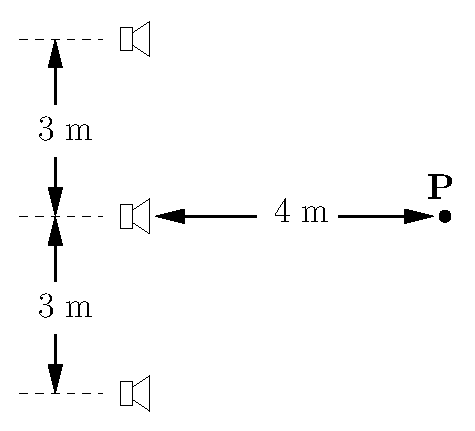
\includegraphics{additional_problems/speakers2}}
      \caption{Problem A\ref{prob:speakers2}}
      \label{fig:speakers2}
    \end{center}
  \end{figure}
  \begin{enumerate}
  \item Draw a phasor diagram representing the sound waves at point
    {\bf P}.  Include a phasor for the wave from each speakers, and a
    phasor for the total wave that results from the superposition of
    these three waves.
  \item Calculate the intensity (in terms of $I_0$) at {\bf P} when
    all three speakers are on.
  \end{enumerate}
\end{aproblem}


\begin{aproblem}{Find the formula.}
  The illustration shows two snapshots of a traveling wave, one taken
  at $t=0\units{s}$ and one taken at $t = 0.25\units{s}$.  Determine a
  formula for the function $y(x,t)$ that describes this traveling
  wave.
  \label{prob:wave_to_eq}
  \begin{figure}[h]
    \begin{center}
      \scalebox{0.65}{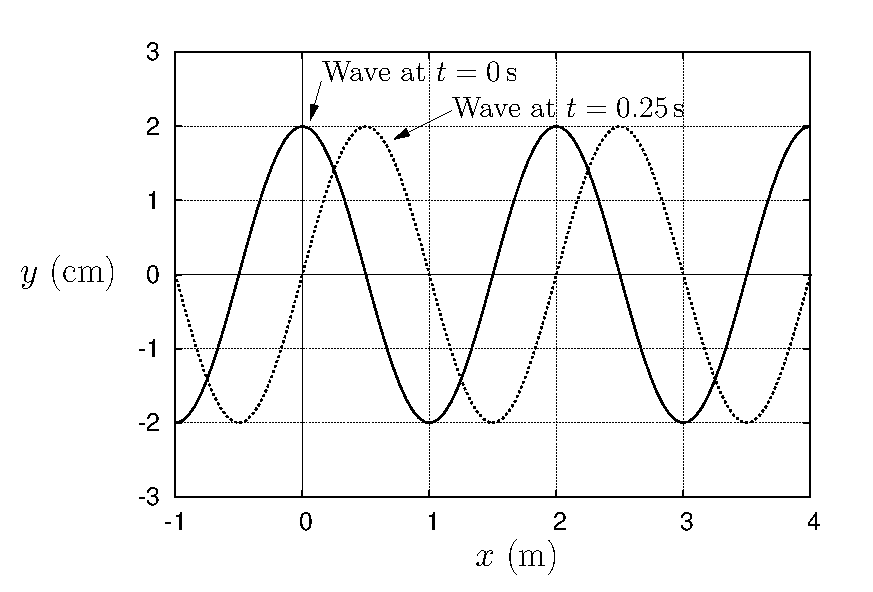
\includegraphics{additional_problems/wave_to_eq}}
      \caption{Problem A\ref{prob:wave_to_eq}}
    \end{center}
  \end{figure}
\end{aproblem}

\newpage

\begin{aproblem}{Adding waves graphically.}
  The graph in Fig.~\ref{fig:wave_to_phasor_1} shows a snapshot of two
  traveling waves at the same instant of time.  The waves have the
  same speed and frequency.  Add these two waves graphically to find
  their sum.

  \label{prob:wave_to_phasor_1}
  \begin{figure}[h]
    \begin{center}
      \scalebox{0.65}{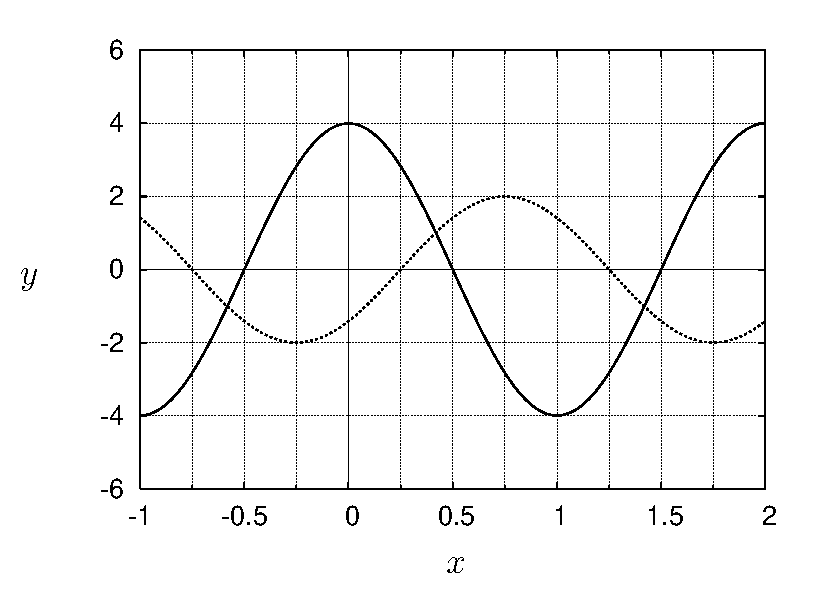
\includegraphics{additional_problems/wave_to_phasor}}
      \caption{Problem A\ref{prob:wave_to_phasor_1}}
      \label{fig:wave_to_phasor_1}
    \end{center}
  \end{figure}

  \vspace{-0.1in}
  {\bf NOTE:} There is no calculation to be performed in this
  graphical addition.  You should be thinking about this as filling in
  entries in a table like the following by reading values from the
  graph, and then plotting the last column, $y_{\rm sum}$ vs. $x$ on
  the graph.
%  \vspace{0.1in}

  \begin{center}
    \begin{tabular}{|c||c|c||c|} \hline
      $x$ & $y_{\rm solid}$ & $y_{\rm dotted}$ & $y_{\rm sum}$ \\ \hline\hline  
      -0.5  & & & \\ \hline
      -0.25 & & & \\ \hline
      0.0   & & & \\ \hline
      0.25  & & & \\ \hline
      \mbox{etc.} & & & \\ \hline
    \end{tabular}
  \end{center}
  \vspace{0.1in}
\end{aproblem}

\begin{aproblem}{Adding waves with phasors.}
  The graph in Fig.~\ref{fig:wave_to_phasor_2} shows a snapshot of two
  traveling waves at the same instant of time.  The waves have the
  same speed and frequency.
  \label{prob:wave_to_phasor_2}
  \begin{figure}[h]
    \begin{center}
      \scalebox{0.65}{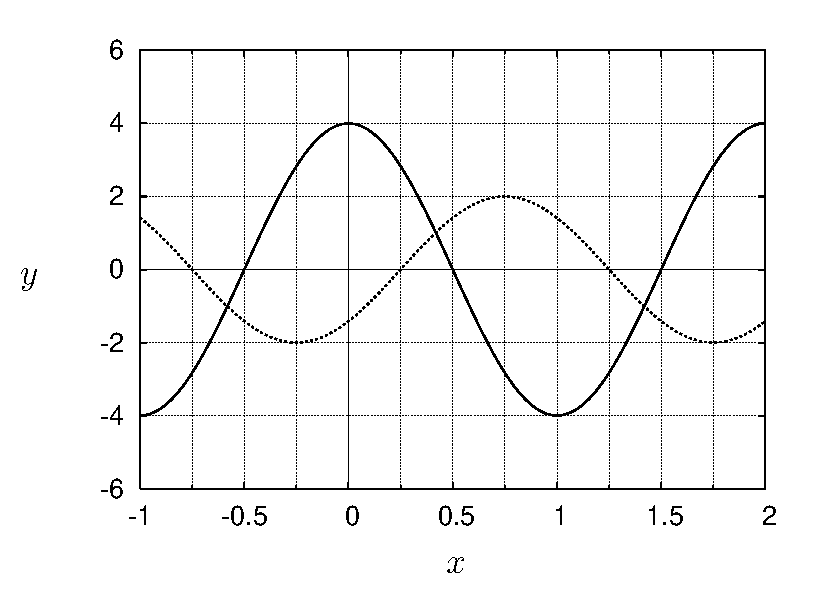
\includegraphics{additional_problems/wave_to_phasor}}
      \caption{Problem A\ref{prob:wave_to_phasor_2}}
      \label{fig:wave_to_phasor_2}
    \end{center}
  \end{figure}

  \begin{enumerate}
  \item Draw two phasors representing these two waves.
  \item Calculate the amplitude of the superposition of these waves.  
  \item Calculate the phase shift of the resultant wave
    with respect to solid wave in the illustration.
  \item Compare your resultant amplitude and phase with the 
    graphical result you got in Problem A\ref{prob:wave_to_phasor_1}.	
  \end{enumerate}
\end{aproblem}


\begin{aproblem}{ Parking Lot.}  
  John, the aspiring physics student/parking attendant (see
  Supp. Ch. 3, Problem \# \ref{prob:parking_lot_1}) gets a job at a
  new hotel that has a more conventional parking lot.  The parking lot
  has a rectangular shape on an $x$-$y$ coordinate system with
  dimensions $100\units{m}\times 50\units{m}$, and the lot is divided
  into three sections, {\bf A}, {\bf B}, and {\bf C} (see figure).
  Although the lot is more conventional, John still tells car owners
  the whereabouts of their cars in terms of probabilities and
  probability densities, only now the probability densities are given
  in terms of {\em probability per unit area} instead of of {\em
    probability per unit length}, and they are functions of two
  variables, $x$ and $y$.
  \label{prob:parking_lot_2}
  \begin{figure}[h]
    \begin{center}
      \scalebox{0.65}{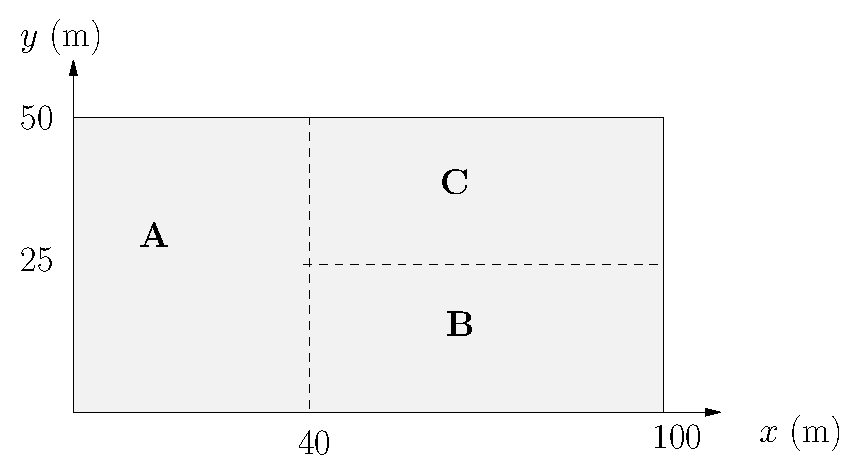
\includegraphics{additional_problems/parking_lot_2}}
      \caption{Problem A\ref{prob:parking_lot_2}}
    \end{center}
  \end{figure}

  \begin{enumerate}
  \item Mr.~Vanderbilt is told that his car ``could be anywhere in the
    lot,'' which means that the probability density is constant
    everywhere (i.e., there is no difference between the sections).
    Calculate the value of this uniform probability density $P(x,y)$
    for Mr.~Vanderbilt to find his car at a position $(x,y)$ on the
    coordinate system of the lot.  (Your answer should be in units of
    probability/m$^2$.)
  \item Find the probability that Mr.~V's car is in section {\bf A} of
    the lot.
  \item Mrs.~Reeve is told that the probability density to find her
    car is a constant $P_A$ in section {\bf A}, a second constant $P_B
    = 4P_A/3$ in section {\bf B}, and a third constant $P_C = 2P_A/3$
    in section {\bf C}.  Find the constants $P_A$, $P_B$, and $P_C$.
  \item Based on your results from part (c), calculate the probability
    that Mrs.~Reeve's car is located in the lower left quarter of the
    lot, i.e, in the region where $0\leq x\leq 50$ and $0\leq y \leq
    25$.
  \end{enumerate}
\end{aproblem}

\begin{aproblem}{Daughter of parking lot.}  
  John, the aspiring physics student/parking attendant (see Problems
  Supp. Ch.~3 \#\ref{prob:parking_lot_1} and {\bf
    A\ref{prob:parking_lot_2}}) gets a job at %yet another hotel, and
  this one has a circular parking lot with radius $40\units{m}$ laid
  out on a $r$-$\theta$ polar coordinate system, and the lot is
  divided into two sections, {\bf A} and {\bf B}.
  \label{prob:parking_lot_3}
  \begin{figure}[h]
    \begin{center}
      \scalebox{0.65}{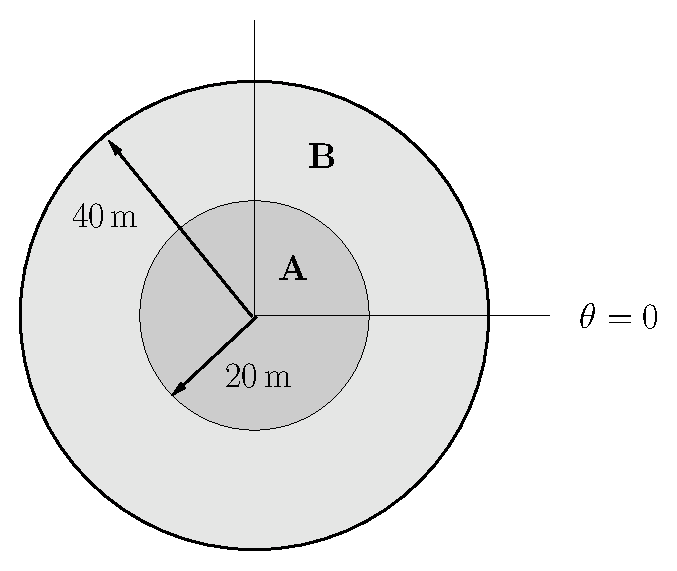
\includegraphics{additional_problems/parking_lot_3}}
      \caption{Problem A\ref{prob:parking_lot_3}}
    \end{center}
  \end{figure}

  \begin{enumerate}
  \item Mr.~Vanderbilt is told that his car ``could be anywhere in the
    lot,'' which means that the probability density is constant
    everywhere (i.e., there is no difference between the sections).
    Calculate the value of this uniform probability density
    $P(r,\theta)$ for Mr.~Vanderbilt to find his car at a position
    $(r,\theta)$ on the coordinate system of the lot.  (Your answer
    should be in units of probability/m$^2$.)
  \item Find the probability that Mr.~V's car is in section {\bf A} of
    the lot.
  \item Mrs.~Reeve is told that the probability density to find her
    car is a constant $P_A$ in section {\bf A} and a second constant
    $P_B = P_A/2$ in section {\bf B}.  Find the constants $P_A$ and
    $P_B$.
  \item Based on your results from part (c), calculate the probability
    that Mrs.~Reeve's car is located within $30\units{m}$ of the
    center of the lot.
  \end{enumerate}
\end{aproblem}


\begin{aproblem}{More practice with complex numbers.}
  \begin{enumerate}
  \item Given the number $z_1 = 0.25$, determine the complex conjugate
    of $z_1$, i.e., determine $z_1^\ast$.
  \item Given the number $z_2 = 0.25i$, determine the complex
    conjugate of $z_2$, i.e., determine $z_2^\ast$.
  \item Given the number $z_3 = 0.5 + 0.3i$, determine the
    magnitude-squared of $z_3$, i.e., determine $\vert z_3\vert^2$.
  \end{enumerate}
\end{aproblem}


\begin{aproblem}{Practice with the complex exponential.}  
  This is a series of exercises that review material from your
  calculus courses, and to give you practice with imaginary numbers in
  an exponent.  Recall from your calculus classes the following Taylor
  series expansions:
  \label{prob:ComplexPractice}
  \begin{eqnarray}
    e^x &=&  1+ x +\frac{x^2}{2!}+\frac{x^3}{3!}+ \frac{x^4}{4!} + \cdots
    \nonumber \\
    \cos x &=& 1 - \frac{x^2}{2!} + \frac{x^4}{4!} + \cdots 
    \nonumber \\
    \sin x &=&  x- \frac{x^3}{3!} + \frac{x^5}{5!} + \cdots
    \nonumber 
  \end{eqnarray}
  
  \begin{enumerate}
  \item Use the expansion for $e^x$ from above, and write a series for
    expression for $e^{i\theta}$, where $\theta$ is a real number.  In
    your answer, don't leave any $i^2$, $i^3$ or $i^4$ factors, (i.e.,
    substitute in the result that $i^2=-1$ whenever possible).

  \item Regroup the terms in your answer from part (a) to show that
    \[  e^{i\theta}=\cos\theta +i\sin\theta.  \]

  \item Use the expansion for $e^x$ from above, and write a series for
    expression for $e^{-i\theta}$, where $\theta$ is a real number.
    In your answer, don't leave any $i^2$, $i^3$ or $i^4$ factors,
    (i.e., substitute in the result that $i^2=-1$ whenever possible)

  \item Regroup the terms in your answer from part (c) to show that
    \[  e^{-i\theta}=\cos\theta - i\sin\theta.  \]

  \item Add the expressions in for $e^{i\theta}$ and $e^{-i\theta}$
    from the results of parts (b) and (d) to show that
    \[ \cos\theta = \frac{e^{i\theta} + e^{-i\theta}}{2}. \]

  \item Find the difference of the expressions for $e^{i\theta}$ and
    $e^{-i\theta}$ from the results parts (b) and (d) to show that
    \[ \sin\theta = \frac{e^{i\theta} - e^{-i\theta}}{2i} = 
    \frac{-i}{2}\left(e^{i\theta} - e^{-i\theta}\right). \]

  \item Write the number $e^{0.5i}$ in the form $a + ib$, where $a$
    and $b$ are real numbers.

  \item Write the number $e^{-0.5i}$ in the form $a + ib$, where $a$
    and $b$ are real numbers.
   
  \item Write the number $e^{0.5i} + e^{-0.5i}$ in the form $a + ib$,
    where $a$ and $b$ are real numbers.

  \item Write the number $e^{0.5i} - e^{-0.5i}$ in the form $a + ib$,
    where $a$ and $b$ are real numbers.

  \item Write the number $\cos(0.3)$ in terms of complex exponentials.

  \item Write the number $\sin(0.3)$ in terms of complex exponentials.

  \item Calculate $|e^{0.3i}|^2$.  Do this two different ways:
    \begin{enumerate}
    \item Write the complex exponential in the form $a + ib$ and find
      the magnitude-squared of this number by multiplying $a+ib$ by
      its complex conjugate.
    \item Find the complex conjugate of $e^{0.3i}$ directly (i.e.,
      leave everything in exponential form) and multiply $e^{0.3i}$ by
      this complex conjugate.
    \end{enumerate}

  \item For reference, calculate $(e^{0.3i})^2$.  (Note that this is
    just squaring rather than taking the magnitude-squared.)  How does
    your answer compare with the result of the previous part?

  \end{enumerate}
\end{aproblem}


\begin{aproblem}{Time-dependent particle-in-box.}   
  Assume that an electron is trapped in a one-dimensional box. The
  energy of the ground state ($|1\rangle$) is $E_1$ and the energy of
  the first excited state ($|2\rangle$) is $4E_1$.  At time $t=0$ the
  electron is in the state
  \[ |\psi(t=0)\rangle = \sqrt{\frac{3}{5}}|1\rangle 
  + \sqrt{\frac{2}{5}}|2\rangle.
  \]
  
  \begin{enumerate}
  \item Calculate the expectation value of the energy for the electron
    at time $t=0$.
  \item Write down the time-dependent state $|\psi(t)\rangle$ (with
    complex exponentials in the coefficients).
  \item Calculate the expectation value of the energy for the electron
    at an arbitrary time $t$.
  \end{enumerate}
  \label{prob:timedependence_1}
\end{aproblem}


\begin{aproblem}{Precessing spins I.}  
  In lecture we considered a particle like a proton (with $s=1/2$ and
  magnetic moment parallel to the spin angular momentum) situated in a
  magnetic field and initially in the state $|\mbox{$+x$}\rangle$, and
  we worked out the time-dependent probabilities for measurements of
  the $x$-component of the spin angular momentum to yield $+\hbar/2$
  and $-\hbar/2$.  In this problem you will repeat the calculation
  done in lecture, but this time for measurements of the $y$-component
  of spin angular momentum.  Don't panic --- we'll take you through
  this step-by-step.
  \label{prob:qm_precess_1}

  \begin{enumerate}

  \item Assume that a particle with magnetic moment $\mu$ starts off
    at time $t=0$ in the state $|\mbox{$+x$}\rangle$; i.e., a
    measurement of $S_x$ would definitely produce a result of $+\hbar
    /2$.  Write down the state $|\psi(0)\rangle$ in terms of the
    ``spin-up'' and ``spin-down'' states $|\mbox{$+z$}\rangle$ and
    $|\mbox{$-z$}\rangle$.

  \item Now assume that the particle is in a magnetic field
    $\vec{B}=B_0 \widehat{k}$.  In a field pointing in the positive
    $z$ direction like this, the states of definite energy are
    $|\mbox{$+z$}\rangle$ and $|\mbox{$-z$}\rangle$.  Write down
    expressions for the energies of these two states.

  \item Use the energies from part (b) to write down an expression for
    the {\em time-dependent} state $|\psi(t)\rangle$.  As a
    short-hand, feel free to use the frequency $\omega \equiv 2\mu
    B_0/\hbar$.

  \item Calculate the probability that a measurement of the
    $y$-component of the spin will give a value $+\hbar/2$.

  \item Calculate the probability that a measurement of the
    $y$-component of the spin will give a value $-\hbar/2$.

  \item Show that the expectation value for measurements of the
    $y$-com\-ponent of spin angular momentum for particles in state
    $|\psi(t)\rangle$ is $(-\hbar/2)\sin(\omega t)$, where $\omega =
    2\mu B/\hbar$.

  \end{enumerate}
\end{aproblem}

\newpage

\begin{aproblem}{Time-dependence of wave functions for particle-in-box.}
  In previous chapters we discussed wavefunctions for particles rather
  than the abstract state-vector representation we have been using for
  properties like ``spin.''  The time dependence of wavefunctions can
  be handled in the same way as the time dependence of spin states.
  First, we write the wavefunction as a normalized linear combination
  of wavefunctions for states with definite energies, and each piece
  of the sum gets a factor of $e^{-iE_it/\hbar}$.  Consider a
  ``particle in a box'' that starts in a linear combination of the
  ground state and the first excited state.  The initial wavefunction
  is
  \[ \psi(t=0) =
  \sqrt{\frac{1}{L}}\sin\left(\frac{\pi x}{L}\right)+
  \sqrt{\frac{1}{L}}\sin\left(\frac{2\pi x}{L}\right), \]
  and at a later time the wave function is
  \[ \psi(t) = 
  e^{-iE_1t/\hbar}\sqrt{\frac{1}{L}}\sin\left(\frac{\pi x}{L}\right)+
  e^{-iE_2t/\hbar}\sqrt{\frac{1}{L}}\sin\left(\frac{2\pi
    x}{L}\right), \] 
  where $E_1 = \frac{h^2}{8mL^2}$ and $E_2 = \frac{h^2}{2mL^2}$ are
  the energies of the two lowest states of a particle in a box. In
  your work for parts (a) and (b) you should leave the energies as
  $E_1$ and $E_2$.

  \begin{enumerate}

  \item Determine the function $|\psi(x,t)|^2$ for the probability
    density as a function of time for this system.

  \item Compare the answer that you got for part (a) here with the
    results from Supplementary Reading Chapter 2, problem 5 and
    comment on the similarities.  (Hint: you should find that the
    answer here alternates in time between the three different
    solutions that you found in Supp.~2-5.)

  \item Download the Excel worksheet \verb+p_in_box.xls+ from the
    calendar page for Lecture 21.  This worksheet plots the
    probability density function that you found in part (b).  Try
    changing the time in the highlighted box at the top -- try $t =
    0$, 0.1, 0.2, 0.3, 0.4, 0.5, $\dots$ up through 2.1.  Comment on
    what you observe with the graphs and what these results imply
    about where you would expect to find the particle after
    measurement of position.
  \end{enumerate}
  \label{prob:time_dependent_wavefunctions}
\end{aproblem}

\newpage

\begin{aproblem}{Precessing spins II.}  
  In this problem you will complete calculations analogous to those
  you performed in problem {\bf A\ref{prob:qm_precess_1}}, except this
  time you will start with the same particle in the state
  $|\mbox{$+y$}\rangle$.

  \begin{enumerate}

  \item Assume that a spin one-half particle with magnetic moment
    $\mu$ oriented parallel to the spin starts off at time $t=0$ in
    the state $|\mbox{$+y$}\rangle$; i.e., a measurement of $S_y$
    would definitely produce a result of $+\hbar /2$.  Write down the
    state $|\psi(0)\rangle$ in terms of the ``spin-up'' and
    ``spin-down'' states $|\mbox{$+z$}\rangle$ and
    $|\mbox{$-z$}\rangle$.

  \item Now assume that the particle is in a magnetic field
    $\vec{B}=B_0 \widehat{k}$.  In a field pointing in the positive
    $z$ direction like this, the states of definite energy are
    $|\mbox{$+z$}\rangle$ and $|\mbox{$-z$}\rangle$.  Write down
    expressions for the energies of these two states.

  \item Use the energies from part (b) to write down an expression for
    the {\em time-dependent} state $|\psi(t)\rangle$.  As a
    short-hand, feel free to use the frequency $\omega \equiv 2\mu
    B_0/\hbar$.

  \item Calculate the probability that a measurement of the
    $y$-component of the spin will give a value $+\hbar/2$.
    
  \item Calculate the probability that a measurement of the
    $y$-component of the spin will give a value $-\hbar/2$.

  \item Show that the expectation value for measurements of the
    $y$-com\-ponent of spin angular momentum for particles in state
    $|\psi(t)\rangle$ is $(\hbar/2)\cos(\omega t)$, where $\omega =
    2\mu B/\hbar$.

  \end{enumerate}
\end{aproblem}

\newpage

\begin{aproblem}{Electric field from a ring of charge.}
  A ring with a radius {\it R} and total charge {\it Q} (distributed
  uniformly) lies in the x-y plane.  Determine the electric field at
  the point {\it P} on the z-axis at a height {\it h} above the center
  of the ring.  {\bf Show all the steps needed to set up and evaluate
    the integral.}
  \label{prob:efield_from_ring}
  \begin{figure}[h]
    \begin{center}
      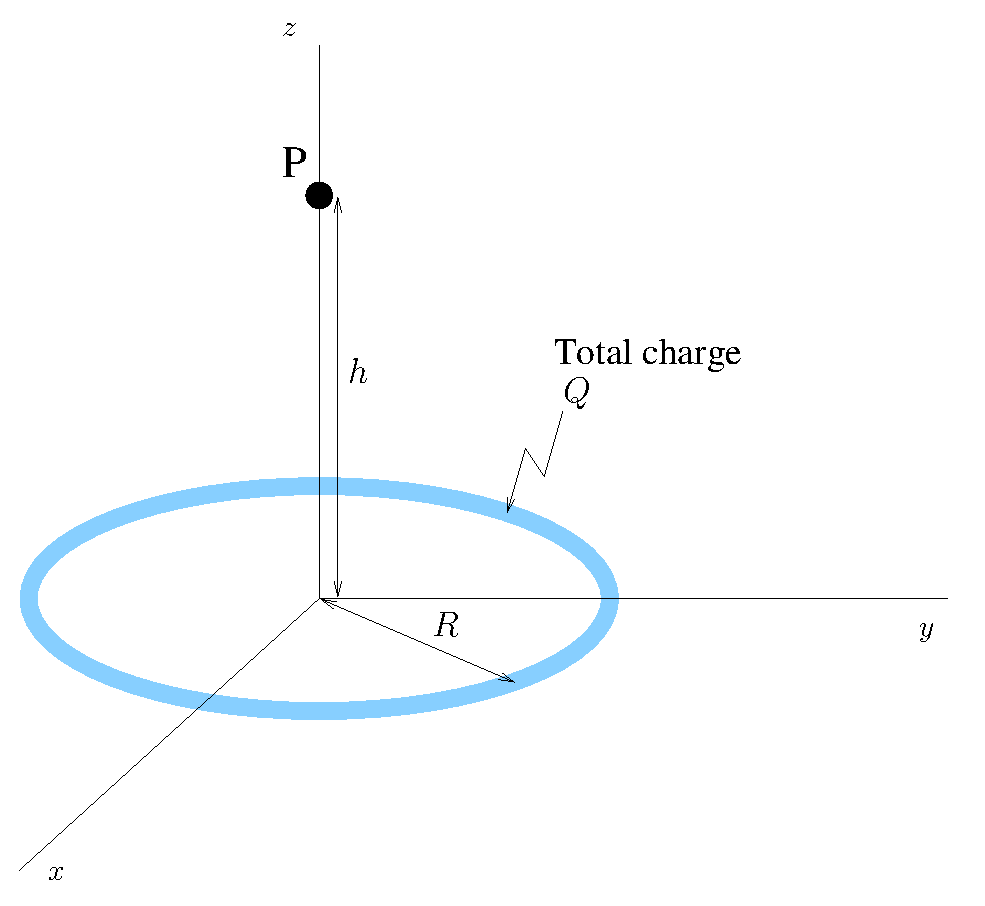
\includegraphics[width=2.4in]{additional_problems/a102fig}
      \caption{Figure for problem A\ref{prob:efield_from_ring}.}
      \label{fig:a102}
    \end{center}
  \end{figure}
\end{aproblem}

\begin{aproblem}{ Phasors and waveforms.}
  The graphs below show snapshots of two traveling waves on a string
  at the same instant of time.
  \label{prob:phasors_and_waveforms}

  \begin{center}
    \includegraphics[width=5.0in]{additional_problems/a103fig}
  \end{center}

  \begin{enumerate}
  \item Draw a phasor diagram which represents the superposition of
    these two waves.  The diagram should be clearly labeled to show
    what represents ``Wave A,'' what represents ``Wave B,'' and what
    represents the superposition of the two (``A+B'').

  \item From the phasor diagram, determine the amplitude of the
    superposition of waves A and B.

  \end{enumerate}
\end{aproblem}

\newpage

\begin{aproblem}{Phasors and waveforms II.}
  The graphs below show snapshots of two traveling waves on a string
  at the same instant of time.

  \begin{center}
    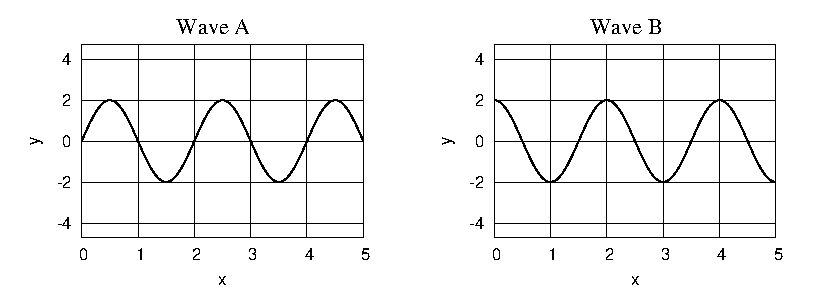
\includegraphics[width=5.0in]{additional_problems/a104fig}
  \end{center}

  \begin{enumerate}
  \item Draw a phasor diagram which represents the superposition of
    these two waves.  The diagram should be clearly labeled to show
    what represents ``Wave A,'' what represents ``Wave B,'' and what
    represents the superposition of the two (``A+B'').

  \item From the phasor diagram, determine the amplitude of the
    superposition of waves A and B.

  \end{enumerate}
\end{aproblem}


\begin{aproblem}{ Radio towers.}
  Three equally spaced AM radio towers are located to the left of a
  receiver as illustrated.  The towers broadcast in-phase radio waves
  of equal amplitude and with wavelength of 500 m.

  \vspace{2mm}
  \begin{center}
    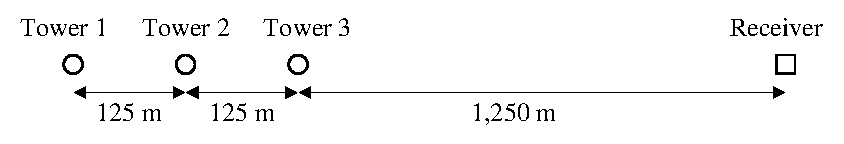
\includegraphics[width=4.5in]{additional_problems/a105fig}
  \end{center}

  \begin{enumerate}

  \item Draw a phasor diagram representing the combined radio wave at
    the receiver.

  \item Assuming the amplitude of the wave reaching the receiver from
    each tower individually is {\em A}, determine the amplitude of the
    combined wave at the receiver.
    
  \end{enumerate}
\end{aproblem}


\newpage

\begin{aproblem}{Feynman fun.}
  Fill in the missing particles (including color and/or charge labels
  where necessary) for the following three Feynman diagrams.
  \label{prob:Feynman_fun}
  \vspace{2mm}
  \begin{center}
    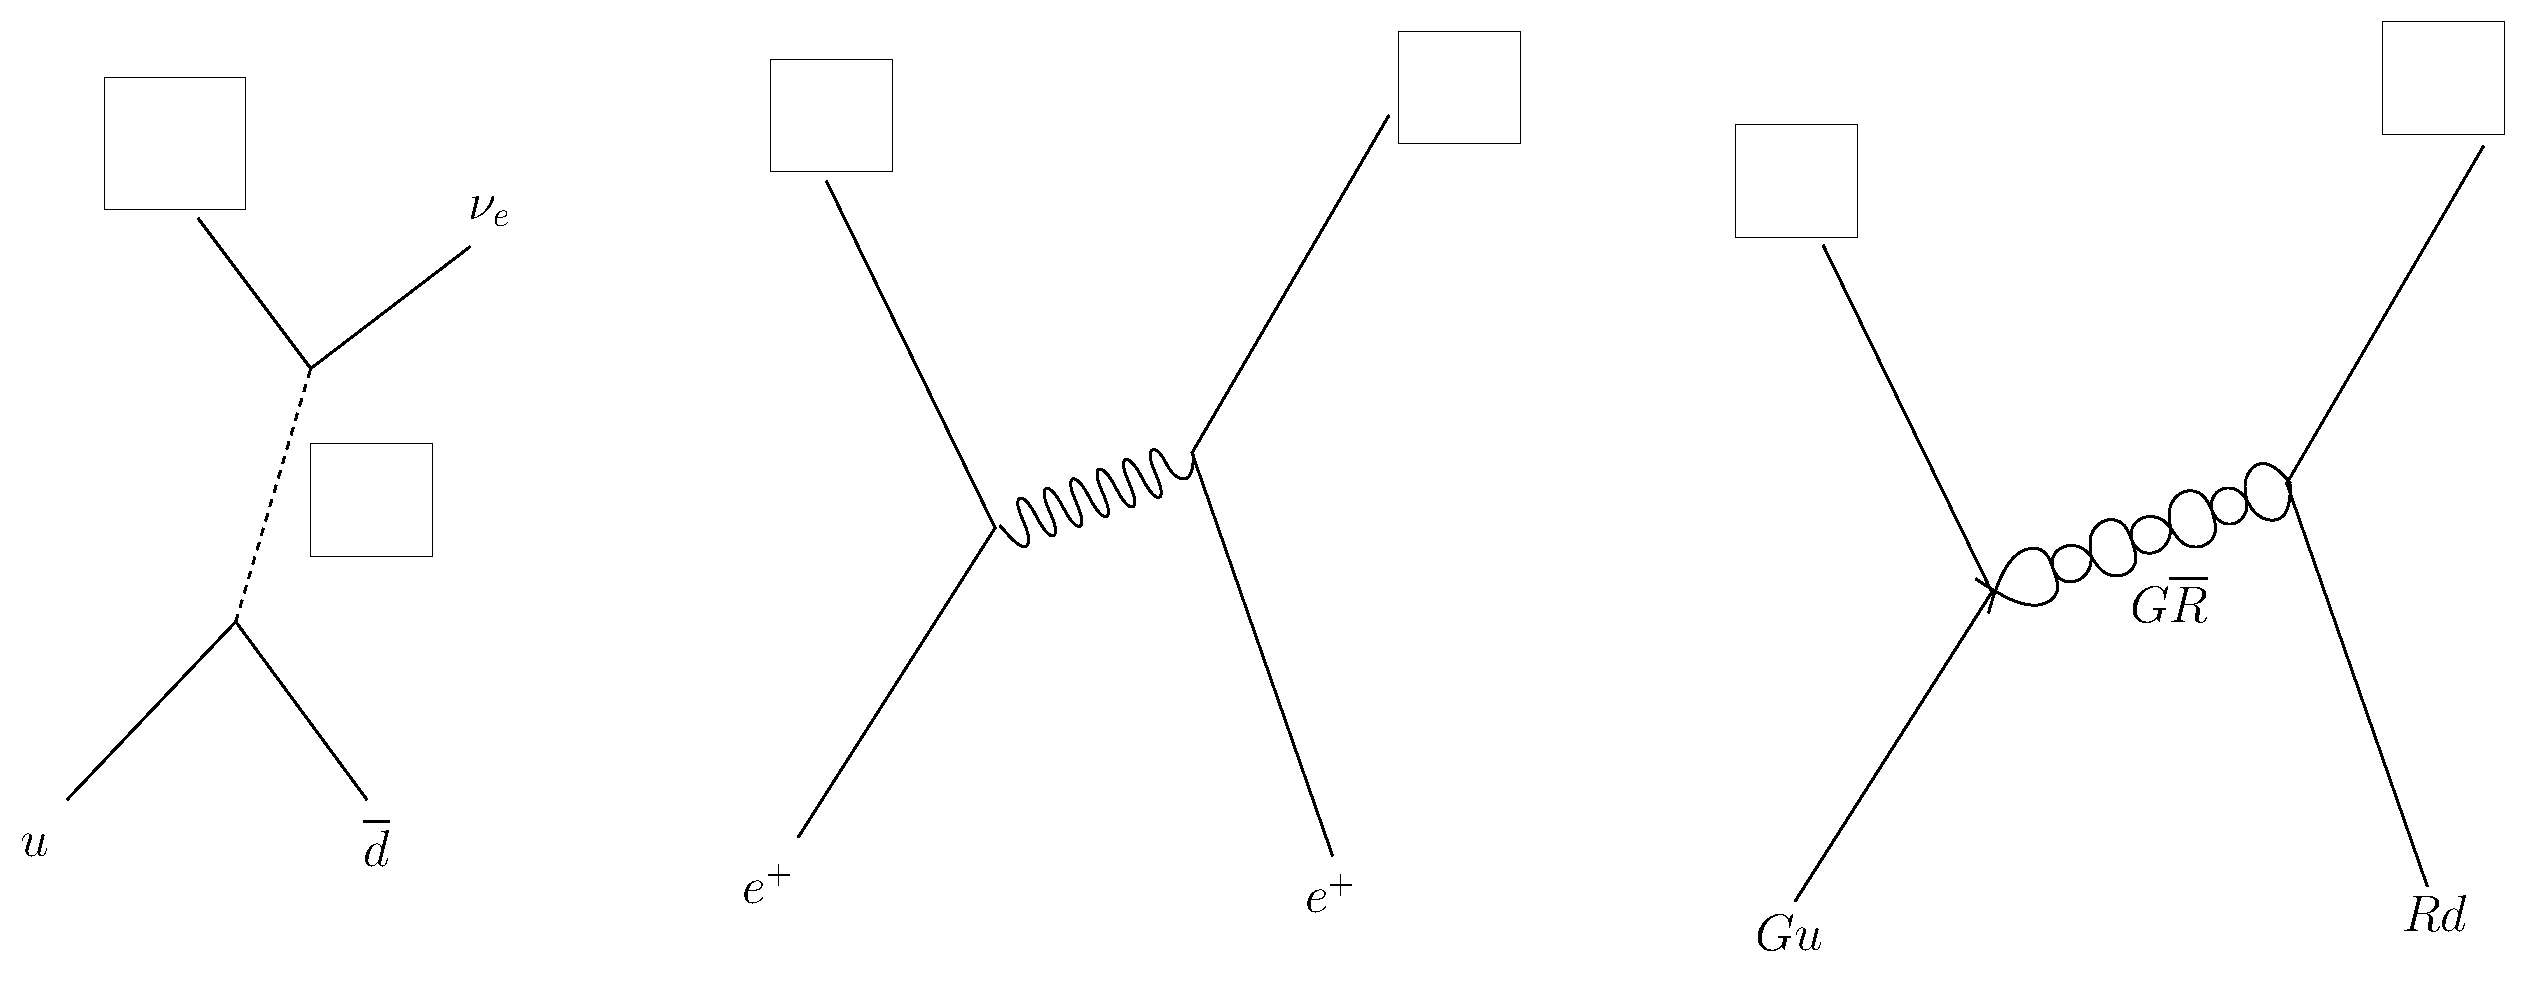
\includegraphics[width=5.4truein]{additional_problems/Feynman_fun}
  \end{center}
  \vspace{2mm}
\end{aproblem}

\begin{aproblem}{Strings and quantum mechanics.}
  This problem compares the time-dependence for a standing wave on a
  string with the time-dependence of the quantum wave function for a
  particle in a box.
  \begin{enumerate}
  \item A string of length $L$ vibrates in its 3rd lowest-frequency
    mode.  Make a sketch of this mode and then write the wavefunction
    in the form
    \[	
    \psi(x) = A \sin (kx),
    \]
    inserting the value of the wave number $k$ that you determine from
    the sketch.

  \item For waves on strings, the angular frequency $\omega$ is
    related to the wave number through $v = \omega / k$. Use this
    relation to write the time-dependent standing wave function,
    \[
    \Psi(x,t) = A \sin (kx) e^{-i\omega t},
    \]
    by expressing both $\omega$ and $k$ in terms of constants and
    properties of the string.

  \item Now consider a particle of mass $m$, confined to 1-D box of
    length $L$ in its third lowest energy state.  Make a sketch of
    this state and then write the wave function in the form
    \[
    \psi(x) = A \sin (kx),
    \]
    inserting the value of the wave number $k$ that you determine from
    the sketch.

  \item For a quantum particle, the angular frequency $\omega$ is
    related to the particle's energy by $E=\hbar\omega$.  For a
    particle free to move within the box, the energy is all kinetic:
    \[
    E=K = \frac{1}{2}mv^2 = \frac{p^2}{2m}= \frac{(\hbar k)^2}{2m}.
    \]
    Use this relation to write the time-dependent quantum
    wavefunction,
    \[
    \Psi(x,t) = A \sin (kx) e^{-iEt/\hbar}
    \]
    by expressing both $E$ and $k$ in terms of constants and
    properties of the particle and the box.
  \end{enumerate}
\end{aproblem}

\begin{aproblem}{Quantum mass-spring.}  
  A quantum mass of $2.5 \times 10^{-10}\units{kg}$ hangs from a
  quantum spring with spring constant $3.5 \times 10^{-5}\units{N/m}$.

  \begin{enumerate}
  \item Recall that classically, the classical angular frequency
    $\omega_c$ of a mass-spring system is independent of amplitude,
    and given by $\omega_c = \sqrt{k_\text{sp}/m}$.  Calculate this
    oscillator's classical period.

  \item The time-dependent quantum wavefunction for this oscillator
    depends on time as $e^{- iEt/\hbar}$ and thus also oscillates.
    Calculate the period of the \textit{wavefunction's} oscillation in
    its 3rd excited state, and compare to your answer in part (a).
  \end{enumerate}
\end{aproblem}


\begin{aproblem}{A square of charges.}
  Three identical charges $q$ and a fourth charge $-q$ form a square
  with sides of length $a$.  Find the electric force vector acting on
  a charge $Q$ placed at the center of the square.
  \label{prob:charges_on_square}

  \begin{figure}[h]
    \begin{center}
      \includegraphics[width=1.75in]{additional_problems/charges_on_square}
    \end{center}
    \caption{Problem A\ref{prob:charges_on_square}.}
  \end{figure}
\end{aproblem}

\newpage

\begin{aproblem}{Parallel currents.}
  Two parallel wires oriented perpendicular to the page are separated
  by $10.0\units{cm}$.  Each wire carries a current of $1.5\units{A}$
  directed out of the page.  Determine the magnitude of the total
  magnetic field at a point {\em P} in the figure, a distance
  $12.0\units{cm}$ above the midpoint of the line connecting the two
  wires.
  \label{prob:two_wires}
  \begin{figure}[h]
    \begin{center}
      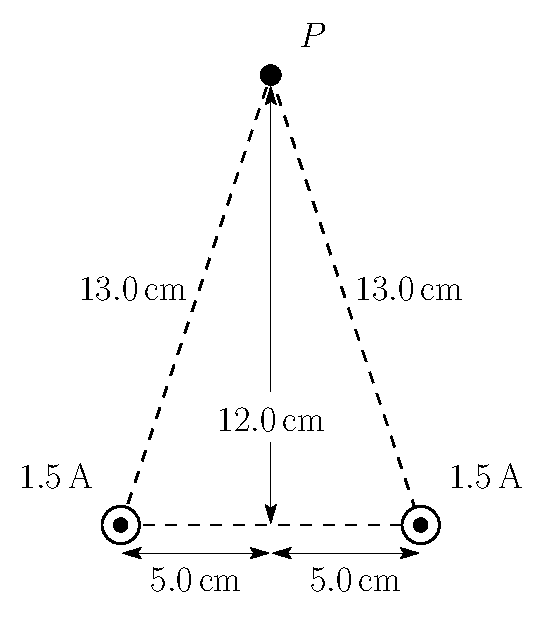
\includegraphics[width=2.in]{additional_problems/two_wires}
    \end{center}
    \caption{Problem A\ref{prob:two_wires}.}
  \end{figure}
\end{aproblem}


\begin{aproblem}{Magnetic field from a wire.}
  A long straight wire $1.0\units{cm}$ in diameter carries a current
  of $5.0\units{A}$ which is evenly distributed over its
  cross-section.  Find the magnetic field strength
  \begin{enumerate}
  \item at a point $5.0\units{mm}$ from the surface of the wire;
  \item at the surface of the wire;
  \item at a point $2.5\units{mm}$ from the axis of the wire.	
  \end{enumerate}
  \label{prob:ampere_wire}
\end{aproblem}


\begin{aproblem}{Whirly Tubes.}  
  Get out your whirly tube and give it a whirl.  Observe it is
  possible to get different notes from it, but not any frequency you
  want; only a certain frequencies seem to be allowed.  Let's
  understand where those are coming from.
  \smallskip

  Your whirly tube has a length of $75\units{cm}$ and is open at both ends.
  \begin{enumerate}
  \item Sketch the standing wave pattern for the three longest
    wavelength modes that fit these end conditions.
  \item From each sketch, determine the corresponding wavelength
    $\lambda$.
  \item Given your answers for (a) and (b), and given the speed of
    sound in air ($340\units{m/s}$), determine the frequency of each
    mode.
  \item Now lets check the values you calculated.  Go the
    website\\ \texttt{plasticity.szynalski.com/tone-generator.htm} and
    enter one of the frequencies you calculated.  How does it compare
    with the sound made when you whirl the tube?  Check all three of
    the frequencies this way.
  \item The sound made by the whirly tube may not perfectly matching
    the calculated frequencies. Some questions: (a) Is the lowest
    frequency note that you are hearing, in fact, the lowest possible
    mode? For some tubes, the lowest note that you hear is actually
    the {\bf second} lowest mode. So, instead of hearing the lowest
    three (1, 2 and 3), you might be hearing modes 2, 3 and 4.  (b)
    The antinodes don't occur exactly at the ends of the tube.  Adjust
    the frequency of the online tone generator up or down until the
    match is better.  What does this tell you?  Are the anti-nodes
    separated by a distance greater 75~cm or less than 75~cm?
  \end{enumerate}
  \label{prob:whirly_tube}
\end{aproblem}

\pagestyle{headings}

\renewcommand{\labelenumi}{\bf \arabic{chapter}.\arabic{enumi}}

%%%%%%%%%%%%%%%%%%%%%%%%%%%%%%%%%%%%%%%%%%%%%%%%%%%%%%%%%%%%%%%%%%%
% Notes (JMH Mar 19, 2014)
% Have added sections on single slit, diffraction limit, and grating
% Still need problems on grating (can be closely modeled on Wolfson problems)
% An example calculation for a diffraction grating
%%%%%%%%%%%%%%%%%%%%%%%%%%%%%%%%%%%%%%%%%%%%%%%%%%%%%%%%%%%%%%%%%%%

\chapter[Phasor Diagrams]{Phasors, Phasor Diagrams, and Wave Interference}
\label{chapter:phasors}
%\setcounter{ex}{0}

\section{Introduction}
\label{sec:phasors_intro}

No, they're not little hand-held devices that can stun and kill
unsuspecting aliens. At least, those aren't the ones we're talking
about here. Phasors provide a way to represent oscillating motion
graphically, and once you understand them a little, they provide for
rather intuitive and straightforward way to handle wave interference
problems.

\section{A Phasor Diagram for a Single Oscillation}
\label{sec:phasor_single}

\begin{figure}\begin{center}
 \includegraphics[width=2.0truein]{phasors/phasor01} 
\caption{\label{fig:phasor01} Mass on a spring.}
\end{center}
\end{figure}


Consider a simple oscillating system, like a mass on a spring moving
back and forth on a frictionless horizontal surface.
We can write an expression for the displacement of the mass as follows:
\begin{equation}
x(t) = A\cos{(\omega t)},
\end{equation} 
where $A$ is the amplitude of the oscillation, and $\omega$ is the
angular frequency in units of rad/s. That means that $A$ is
the value of the largest deviation (plus or minus) of the mass from
its equilibrium position, and the value of $\omega$ governs the time it
takes for the mass to complete one oscillation (recall that the period
of the oscillation, $T = 2\pi/\omega$, so a small $\omega$
means a long period while a large $\omega$ means a short period).
Together, $A$ and $\omega$ completely define the oscillation.


We can represent these two quantities, and therefore the oscillation
itself, with a phasor diagram. A phasor is nothing more than a vector
with magnitude $A$ that {\em rotates} with angular velocity $\omega$. The
concept of a rotating vector is a little strange, but it works out really
well for oscillations.  For the oscillation defined above, $x(0) = A$
since $\cos{(0)} = 1$. We can represent the oscillation at this time
with a phasor of length $A$ that lies on the horizontal axis, as seen
in Fig.~\ref{fig:phasor02}.

\begin{figure}\begin{center}
 \includegraphics[width=4.0truein]{phasors/phasor02} 
\caption{\label{fig:phasor02}Oscillator and phasor at time $t=0$.}
\end{center}
\end{figure}

Not very interesting yet, I know, but here's the cool part: let time
advance.  As time passes, the mass moves back toward its equilibrium
position. At the same time, the phasor rotates in the counterclockwise
direction. The phasor's magnitude doesn't change, but the projection
of the phasor onto the horizontal axis (i.e., the horizontal
component of the vector describing the phasor) gets smaller, as 
shown in Fig.~\ref{fig:phasor03}.

\begin{figure}\begin{center}
 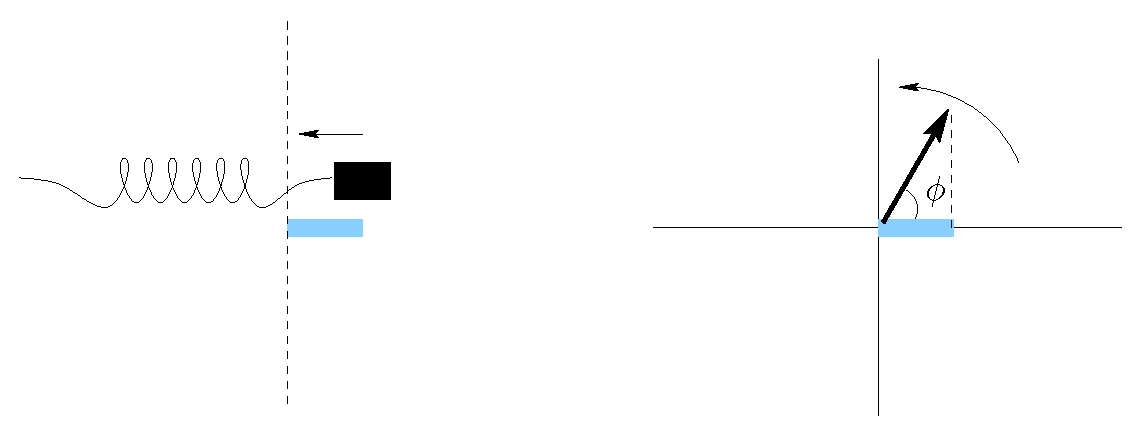
\includegraphics[width=4.0truein]{phasors/phasor03} 
\caption{\label{fig:phasor03}Oscillator and phasor a little bit later.}
\end{center}
\end{figure}

\begin{figure}\begin{center}
 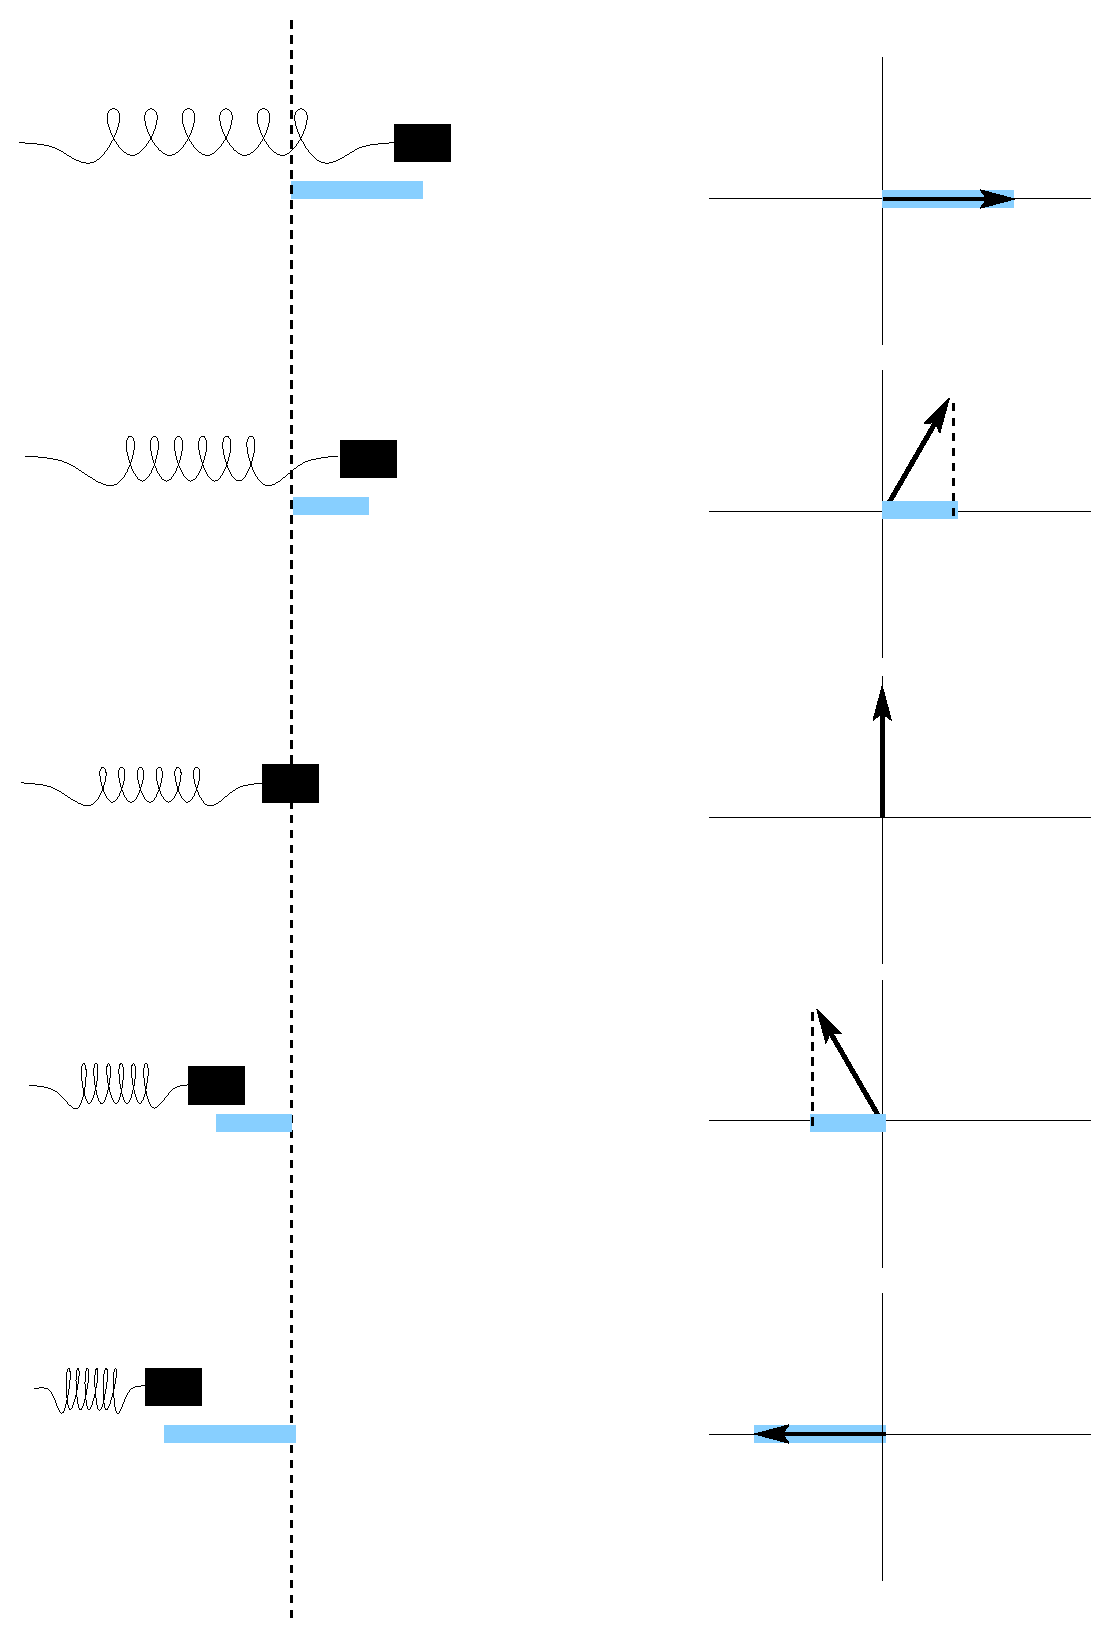
\includegraphics[width=4.0truein]{phasors/phasor04} 
\end{center}\caption{\label{fig:phasor04}Time evolution of the oscillator
and corresponding phasor.}
\end{figure}


Now if $\phi = \omega t$ in the phasor diagram, then the projection of
the phasor on the horizontal axis is $A\cos{(\phi)} = A\cos{(\omega
  t)}$, and that's precisely the expression for the displacement of
the mass at time $t$. This means that if the phasor rotates with
angular velocity $\omega$ and starts in the horizontal position at $t
= 0$, its projection onto the horizontal axis will always describe the
displacement of the oscillation, as seen in Fig.~\ref{fig:phasor04}.


Note that the phasor does not change length; rather, it's just the
projection of the phasor onto the horizontal axis that changes to
describe the oscillation's changing displacement.  This diagram should
also give you a better idea of why we talk about ``angular frequency''
for oscillations. We're matching up the frequency of the oscillation
with the angular velocity of the rotating phasor.

%%\newpage
\begin{example}{A Day at the Beach.} 
\label{example1}
Imagine you're at the beach and you walk into the surf
until you're waist-deep in the water. You feel the waves passing by
you, and you realize that you can express the change in the level of
the water at your location with the expression
\begin{equation}
y(t) = A\cos{(\omega t)},
\end{equation} 
where $A = 20\units{cm}$ and $\omega = \frac{\pi}{3}\units{rad/s}$.
Draw a phasor diagram to depict the level of the water at time
$t = 3\units{s}$.
%\solution
\begin{solution}
The phasor describing this oscillation will have magnitude $A = 20\units{cm}$,
so we need a vector of that length. At time $t = 3\units{s}$, the
phasor will have rotated so that
\begin{equation}
\phi (t) = \omega t = \frac{\pi}{3}\times 3 = \pi\units{rad}. 
\end{equation}
The phasor diagram is illustrated in Fig.~\ref{fig:phasor05}. 
\noindent The projection of the phasor onto the horizontal axis is
$-20\units{cm}$, so at this time, the wave height is at a minimum
(i.e., a trough).

\begin{figure}
\begin{center}
 \includegraphics[width=2.5truein]{phasors/phasor05} 
\caption{Phasor diagram for Example~\ref{example1}.
\label{fig:phasor05}}
\end{center}
\end{figure}


{\em Important Note:} Even though this problem is about an oscillation
in the vertical direction, I still measure the displacement of the
oscillation by the projection of the phasor onto the {\em horizontal}
axis. There is no $x$-  or $y$-axis on a phasor diagram, so don't go
and try to match up the orientation of the oscillation with the phasor
diagram.
\end{solution}
\end{example}

%\newpage

\begin{exampleb}{Alarm Bells.} 
\label{example2}
A fire alarm goes off in your dorm. You run outside and stand in the 
cold weather waiting for the fire department to
arrive and turn off the alarm (it's yet another false alarm). While
you're waiting, you get out your pocket oscilloscope and measure the
change in density of the air at your location due to the compression
from the sound waves from the fire alarm. You measure the density
change $\Delta \rho(t)$ to be described by the following expression:
\begin{equation}
\Delta \rho(t) = A\cos{\left(\omega t + \phi_0\right)},
\end{equation} 
where $A = 0.012\units{kg/m$^3$}$, $\omega =5000\pi\units{rad/s}$, 
and $\phi_0 = \frac{\pi}{4}$. You decide to draw a phasor diagram 
describing the density at time $t= 0.1\units{ms}$.
%\solution
\begin{solution}
This problem is a little trickier because of the non-zero $\phi_0$
inside the cosine. Conceptually, it means that when you decided to
define time $t=0$, the oscillation wasn't at a maximum. Instead, at
time $t=0$,
\begin{equation}
\Delta \rho(t) = A\cos{(\phi_0)} 
                  = 0.012\, \cos{\left(\frac{\pi}{4}\right)}
                  = 0.0085\units{kg/m$^3$}.
\end{equation}
\begin{figure}[b]
\begin{center}
 \includegraphics[width=2.75truein]{phasors/phasor06} 
\caption{\label{fig:phasor06}Phasor corresponding to an oscillator
with a phase shift.}
\end{center}
\end{figure}
There's nothing wrong with this, but it will affect how we draw our
phasor diagram. The amplitude of the oscillation is %still 
$A = 0.012\units{kg/m$^3$}$, so that must be the length of our phasor.
However, if the projection of this phasor onto the horizontal axis at
time $t = 0$ is to be $0.0085\units{kg/m$^3$}$, then the phasor must
be rotated. By how much? By $\phi_0$ (see Fig.~\ref{fig:phasor06}).

Fig.~\ref{fig:phasor06} is the ``starting point'' for our phasor diagram. To
produce the phasor diagram for $t = 0.1\units{ms}$, we need to let
this phasor rotate for that time interval. It will rotate by
\begin{equation}
\Delta \phi(t) = \omega t = 5000\pi\times 0.0001 = \frac{\pi}{2}
\end{equation} 
{\em from the starting point} of $\phi_0 = \frac{\pi}{4}$.
So our phasor diagram will look like Fig.~\ref{fig:phasor07}. %this:

\begin{figure}\begin{center}
 \includegraphics[width=2.5truein]{phasors/phasor07} 
\caption{\label{fig:phasor07}Phasor diagram of oscillator in
Example~\ref{example2} at $t=0.1$}
\end{center}
\end{figure}

The projection of the phasor at this time is
\begin{equation}
A\cos{\left(\frac{3\pi}{4}\right)} = -0.0085\units{kg/m$^3$}. 
\end{equation}
That's the same value we get from the algebraic expression for 
$\Delta \rho (t)$:
\begin{eqnarray}
\Delta \rho (t) & = & A \cos{\left( \omega t + \phi_0\right)}\nonumber\\
               & = & 0.012\, \cos{\left(5000\pi\times 0.1 
                    + \frac{\pi}{4}\right)} \nonumber\\
               & = & 0.012\, \cos{\left(\frac{3\pi}{4}\right)}\nonumber\\
               & = &  -0.0085\units{kg/m$^3$}.
\end{eqnarray}
The change in density at this moment is negative, so the density is
lower than its equilibrium value due to the passing sound wave.
\end{solution}
\end{exampleb}


\section{Phasors as Complex Numbers}
\label{sec:phasor_complex_notation}

You may have encountered complex numbers in your math classes.
Recall that a complex number $z$ can be written as
\begin{equation}
z = a + ib
\end{equation}
with $a$ and $b$ real numbers, and that $i$ is the imaginary unit, 
$i = \sqrt{-1}$.  Here $a$ is called the \textit{real part} of  $z$ 
[written $\mbox{Re}(z)$], while $b$ is called the \textit{imaginary part} 
of $z$ [written $\mbox{Im}(z)$].

It's easy to represent a complex number  graphically.  Just plot the 
real part complex number along the horizontal, or real axis, 
and the imaginary part along the vertical, or imaginary axis,
as shown in Fig.~\ref{fig:complexPlane}.

\begin{figure}\begin{center}
\includegraphics[width=2.2in]{phasors/complex_plane}  
\caption{\label{fig:complexPlane} A complex number can be represented
graphically as a point in the complex plane.}
\end{center}
\end{figure}

The length of the diagonal line from the origin to the point representing
the complex number $z$ is the \textit{magnitude} of $z$, and corresponds
the amplitude of the oscillation $A$, and the angle with respect to the 
positive real axis corresponds to the phase angle $\phi$, as shown in 
Fig.~\ref{fig:complexPhasor}, which is really just a phasor diagram!
\begin{figure}[b]
\begin{center}
\includegraphics[width=2.2in]{phasors/complex_phasor}  
\caption{\label{fig:complexPhasor}Phasors correspond to complex numbers.}
\end{center}
\end{figure}

Applying simple trig to the diagram gives 
\begin{equation}
a = \mbox{Re}(z) = A \cos\phi\hspace{0.5in}b = \mbox{Im}(z) = A\sin\phi.
\end{equation} 
It is the real part of the complex number that corresponds to the 
physical oscillation,  but using the complex representation actually 
simplifies many calculations.  

The connection to phasors gets even stronger when we make use of the 
Euler identity
\begin{equation}
e^{i\phi} = \cos\phi + i\sin\phi,
\label{eq:euler}
\end{equation}
so that
\begin{eqnarray}
z = a + ib &=& A\cos\phi + i A\sin\phi \nonumber \\
	   &=& A(\cos\phi + i\sin\phi)  \nonumber \\
  	   &=& Ae^{i\phi}.
\end{eqnarray}
Thus, if we have an oscillation represented in complex exponential form,
we can immediately draw its phasor picture:  Make an arrow of length
$A$ at angle $\phi$ from the real (horizontal) axis.

\begin{example}{Another Day at the Beach.}  
\label{example3}
The change in water level at your location is now represented with
the following complex function (whose real part is the actual water
height):
\begin{equation}
y(t) = 25 \, e^{i(\pi/4\, t + \pi/2)},
\end{equation}
with $y$ in cm and $t$ in sec. 
Draw a phasor diagram to depict the level of the water at $t = 2$, 3 and 
$4\units{s}$.
\solution
Draw the real and imaginary axes.  Starting at the real axis, 
go counterclockwise for $\pi/2$ radians (the phase constant $\phi_0$).  
Then keep going counterclockwise $\pi/4$ radians for each second of 
elapsed time.  The phasors are shown in Fig.~\ref{fig:phasorRotation}.

\begin{figure}
\begin{center}
 \scalebox{0.6}{\includegraphics{phasors/phasor_rotation}}  
\caption{\label{fig:phasorRotation}Phasors for the water level in 
Example~\ref{example3} at times $t=2\units{s}$, $t=3\units{s}$, and 
$t=4\units{s}$.}
\end{center}
\end{figure}
To find actual water levels, take the real part (the horizontal projection).  
The water levels are thus   
\begin{eqnarray}
&&\mbox{at $t=2\units{s}$}: \hspace{0.5in}-25\units{cm}\nonumber \\
&&\mbox{at $t=3\units{s}$}: \hspace{0.5in}-25\cos(\pi/4)= 
  -\frac{25}{\sqrt{2}}\simeq-17.7\units{cm}\nonumber\\ 
&&\mbox{at $t=4\units{s}$}:\hspace{0.5in}0\nonumber
\end{eqnarray}
\end{example}

\section{Adding Phasors}
\label{sec:adding_phasors}

\begin{figure}[b]
\begin{center}
\includegraphics[width=4.2truein]{phasors/phasor08} 
\caption{\label{fig:phasor08}Phasor diagram showing separate phasors 
for oscillations $y_1$ and $y_2$ rotating together with the 
same angular frequency.}
\end{center}
\end{figure}
%

The power and utility of the phasor representation really show up
when combining oscillations. Consider two oscillations, both with the
same angular frequency $\omega$, but with different amplitudes and
phases:
\begin{equation}
y_1(t) = A_1\cos{(\omega t + \phi_1)}\quad \text{and} \quad
y_2(t) = A_2\cos{(\omega t + \phi_2)}.  
\end{equation}
The superposition of these two oscillations, $y_{\rm tot} = y_1 + y_2$,
will be sinusoidal with the same angular frequency $\omega$, 
but it is very messy to calculate the new amplitude and phase shift  
algebraically; it is actually much simpler
using the complex phasor method. Because the oscillation's have 
the same frequency, the phasors rotate together as time passes,
as illustrated in Fig.~\ref{fig:phasor08}.  That is, the angle
between the phasors will always be $\Delta\phi = \phi_2-\phi_1$.

%\begin{figure}\begin{center}
% \includegraphics[width=2.4truein]{phasors/phasor08a} 
%\caption{\label{fig:phasor08a}Phasor diagram
%showing phasors for oscillations $y_1$ and $y_2$ at a later time $t=t_0$.
%}
%\end{center}
%\end{figure}


The resultant phasor, with its own amplitude and phase, is illustrated
in Fig.~\ref{fig:phasor09}.  We can determine the amplitude and phase
of the resultant phasor by adding the two input phasors the same way we
add vectors.  The amplitude of the resultant will be less than the sum
of the two original phasor amplitudes (unless $\Delta\phi = 0$) and the
phase of the resultant will be something between the phases of the two
original phasors.

\begin{figure}
\begin{center}
 \includegraphics[width=2.0truein]{phasors/phasor09} 
\caption{\label{fig:phasor09}The combined oscillation is described by 
a phasor that is the vector sum of the two separate phasors.}
\end{center}
\end{figure}

\begin{example}{Rock Your Boat.} 
\label{example4}
You're sitting in a boat in the middle of a calm lake. Suddenly a motor
boat drives by, producing waves that would oscillate your boat up and
down as follows:
\begin{equation}
y_1(t) = A_1\cos{(\omega t + \phi_1)}, 
\end{equation}
where $A_1 = 25\units{cm}$, $\omega = \frac{2\pi}{3}$, and
$\phi_1 = \frac{\pi}{6}$. At the same time, another motor boat drives
by, producing waves that would oscillate your boat up and down as follows:
\begin{equation}
y_2(t) = A_2\cos{(\omega t + \phi_2)}, 
\end{equation}
where $A_2 = 15\units{cm}$, $\omega = \frac{2\pi}{3}$, and
$\phi_1 = \frac{\pi}{3}$. However, since both waves act on the boat
simultaneously, the actual oscillation of your boat is the
superposition of these two waves. How much does your boat move up and
down as a result of the combination of these waves?
\solution
The phasor diagram for these two separate oscillations %looks like this:
is shown in Fig.~\ref{fig:phasor10}.
The resultant phasor can be determined from the vector addition of the
phasors shown in Fig.~\ref{fig:phasor11}.

\renewcommand{\arraystretch}{2.0}
\begin{center}
\begin{tabular}{|c|c|c|}\hline
\quad Phasor\quad &
\quad real part (horizontal) \quad &
\quad imaginary part (vertical) \quad \\ 
\hline\hline
1      & $25\cos\left(\frac{\pi}{6}\right) = 21.6$ 
       & $25\sin\left(\frac{\pi}{6}\right) = 12.5$ \\ \hline 
2      & $15\cos\left(\frac{\pi}{3}\right) =7.5$ 
       & $15\sin\left(\frac{\pi}{3}\right) =13.0$ \\
\hline\hline
Total  & $29.1$   & $25.5$ \\
\hline
\end{tabular}
\end{center}
\renewcommand{\arraystretch}{1.0}

\begin{figure}\begin{center}
 \includegraphics[width=2.0truein]{phasors/phasor10} 
\caption{\label{fig:phasor10}Phasor diagram for 
two water waves in Example~\ref{example4}. }
\end{center}
\end{figure}

\noindent So, the amplitude of the resultant phasor is 
\begin{equation}
A_{\rm tot} = \sqrt{29.1^2 + 25.5^2} =38.7\units{cm}, 
\end{equation} 
and its initial phase is 
\begin{equation}
\phi_{\rm tot} = \tan^{-1}{\left(\frac{25.5}{29.1}\right)} 
                  = 0.72\units{rad}.  
\end{equation} 

\begin{figure}[b]
\begin{center}
 \includegraphics[width=2.0truein]{phasors/phasor11} 
\caption{\label{fig:phasor11}Phasor addition  for 
two water waves in Example~\ref{example4}.}
\end{center}
\end{figure}
We can write the superposition as
\begin{eqnarray*}
 y_{\rm tot}(t) & = & A_{\rm tot}\cos{(\omega t + \phi_{\rm tot})} \\
            & = & 38.7\cos{(\omega t + 0.72)}, \\
\end{eqnarray*}
with $y$ in cm and $t$ in sec.
\end{example}
\newpage

\begin{exampleb}{Two Towers.} 
\label{exampleTwoTowers}
\begin{figure}\begin{center}
 \includegraphics[width=3.0truein]{phasors/phasor12} 
\caption{\label{fig:phasor12}Illustration of radio towers in 
Example~\ref{exampleTwoTowers}.}
\end{center}
\end{figure}
Two radio towers, A and B, separated by $20\units{m}$,
broadcast the same radio signal of wavelength $\lambda =
12\units{m}$. You're standing at the point $P$ indicated in the
figure with your radio wave amplitude meter.
With only tower A broadcasting, you measure a wave amplitude
of 7 (in some unspecified unit).  With only tower B broadcasting, you
measure a wave amplitude of 5. What amplitude do you measure when both
towers are broadcasting?
\solution
Here we're interested in the superposition of the waves from the two
towers. We aren't explicitly given the phase difference between the
wave signals that arrive at $P$ from the two towers, but we can figure
it out because we know the distances from point $P$ to each tower. If
the waves leave the two towers in phase, they won't necessarily be in
phase when they reach point $P$ because the waves from Tower B have to
travel farther. How much farther? Well, the distance between Tower B
and point $P$ is $\sqrt{50^2 + 20^2} = 53.85\units{m}$, so the waves
from Tower B have to travel $3.85\units{m}$ farther. That means the
waves from Tower A will be $3.85\units{m}$ ahead of the waves from
Tower B.

We can turn that distance difference into a phase difference for the
waves. The path length difference $\Delta r = 3.85\units{m}$ produces
$\frac{3.85}{12} = 0.32$ {\em wavelengths} of difference between the two
waves as they arrive at point $P$.
If the waves from Tower A arrived exactly one wavelength ahead of the
waves from Tower B, the signals would add constructively. The phase
difference would be $2\pi$, and peaks and troughs of the two waves
would be aligned. In this case, however, the waves from Tower A arrive
only $0.32\units{wavelengths}$ ahead of the waves from Tower B.
Consequently, the phase difference $\Delta\phi$ is
\begin{equation}
\Delta\phi = 2\pi \frac{\Delta r}{\lambda} = 2\pi \frac{3.85}{12} 
= 2.0\units{rad}.
\end{equation} 
We can then write expressions for the two oscillations at point $P$ as
follows:
\begin{equation}
y_A(t) = 7\cos{\left(\omega t + 2.0\right)} \quad\quad
 y_B(t) = 5\cos{\left(\omega t\right)}.
\end{equation}
Why did I pick zero initial phase for the signal from Tower B?
Because I could. In this case (and in most cases we'll deal with),
we're only interested in the phase difference between signals.
Therefore, I can always choose to describe one wave with zero initial
phase, and then put the phase difference into the expression for the
other wave. With one phasor on the horizontal axis, the phasor
addition is just easier.

Now we can construct a phasor diagram for the two oscillations, shown
in Fig.~\ref{fig:phasor13}.

\begin{figure}\begin{center}
 \includegraphics[width=2.4truein]{phasors/phasor13} 
\caption{\label{fig:phasor13}Phasor diagram for radio waves in 
Example \ref{exampleTwoTowers}.}
\end{center}
\end{figure}

Once again, the resultant phasor can be determined from the vector
addition of the phasors.

\renewcommand{\arraystretch}{2.0}
\begin{center}
\begin{tabular}{|c|c|c|}\hline
\quad Phasor\quad\mbox{} &
\quad real part (horizontal) \quad \mbox{}&
\quad imaginary part (vertical) \quad\mbox{} \\ 
\hline\hline
1      & $5\cos{\left(0\right)}=5$ & $5\sin{\left(0\right)}=0$ \\
\hline
2      & $7\cos{\left(2.0\right)}=-2.9$ & $7\sin{\left(2.0\right)}=6.4$ \\
\hline\hline
Total  & $2.1$   & $6.4$ \\
\hline
\end{tabular}
\end{center}
\renewcommand{\arraystretch}{1.0}
\vspace{0.08in}

So, the amplitude of the resultant phasor is 
\begin{equation}
A_{\rm tot} = \sqrt{2.1^2 + 6.4^2} = 6.7,
\end{equation}
and its initial phase is
\begin{equation}
\phi_{\rm tot} = \tan^{-1}{\left(\frac{6.4}{2.1}\right)} 
      = 1.25\units{rad},
\end{equation} 
and we can thus write the superposed oscillation as
\begin{equation}
y_{\rm tot}(t) = 6.7\cos{(\omega t + 1.25)}. 
\end{equation}
\end{exampleb}

\section[Multi-Source Interference]{Phasor Diagrams for Multiple Source Interference}
\label{sec:phasors_multiple_source}

Sometimes, more than two waves will interfere at a single point. In
these cases, the total amplitude of the combined oscillation will be
the superposition of all of the incident waves. The phasor addition
technique can be used to calculate the total amplitude in these
complicated cases. Consider, for example, three oscillations, all with
the same angular frequency $\omega$, but with different amplitudes and
phases:

\begin{eqnarray*}
y_1(t) & = & A_1\cos{(\omega t + \phi_1)}, \\
y_2(t) & = & A_2\cos{(\omega t + \phi_2)}, \ {\rm and} \\
y_3(t) & = & A_3\cos{(\omega t + \phi_3)}.
\end{eqnarray*}
These three oscillations can be expressed graphically, as shown in 
Fig.~\ref{fig:phasor15},
 and their superposition, $y_{\rm tot} = y_1 + y_2 + y_3$, can
be determined from vector addition of the three phasors.


\begin{figure}\begin{center}
 \includegraphics[width=2.4truein]{phasors/phasor15} 
\caption{\label{fig:phasor15}Phasors for the three oscillations $y_1$, $y_2$, 
and $y_3$.}
\end{center}
\end{figure}
%\noindent 

One of the most common multi-source interference problems is an
extension of the two-slit problem considered in class. Imagine a light
source passing through a screen containing not two but {\em three}
slits, each separated from its neighbor by a distance $d$, as shown
in Fig.~\ref{fig:phasor16}.
 The interference pattern for this arrangement of slits will
look different from the interference pattern for a two-slit setup.


\begin{figure}\begin{center}
 \includegraphics[width=3.0truein]{phasors/phasor16} 
\caption{\label{fig:phasor16}Three closely spaced slits, illuminated straight-on
from the right. The interference pattern is observed on a distant screen to the right.}
\end{center}
\end{figure}



\begin{figure}\begin{center}
 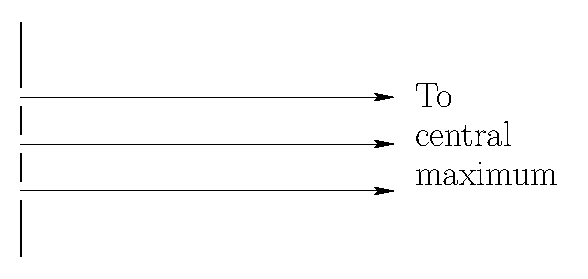
\includegraphics[width=2.0truein]{phasors/phasor17} 
\caption{\label{fig:phasor17}Light rays exiting the three slits
parallel to the normal.}
\end{center}
\end{figure}


If the interference pattern illuminates a screen a distance $L$ from
the slits, where $L\gg d$, then we can assume that the light rays from
each of the slits to any particular point on the screen are parallel.
(This is the same approximation we made in the two-slit case.) For
example, light passing straight through the slits and continuing
straight to the screen produce the central maximum in the interference
pattern, as in Fig.~\ref{fig:phasor17}.
 These rays combine constructively because there's no
difference in the path length for the three light rays, i.e., $\Delta
r = 0$ for all three rays.

Now consider the light rays traveling at an angle $\theta$ to the normal,
as in Fig.~\ref{fig:phasor18}.
 Just as in the two-slit case, these rays do not travel the
same distance to reach the screen. Light from the bottom slit travels
the shortest distance, while light from the middle slit travels an
extra distance $\Delta r_{21}$, and light from the top slit travels
the same amount of extra distance ($\Delta r_{32} = \Delta r_{21}$)
compared to light from the middle slit (Here, I've implicitly labeled
the slits, \#1, 2, and 3 for bottom, middle, and top.).


\begin{figure}\begin{center}
 \includegraphics[width=2.0truein]{phasors/phasor18} 
\caption{\label{fig:phasor18}Light rays exiting at an angle $\theta$ to
the normal.}
\end{center}
\end{figure}


\begin{figure}\begin{center}
 \includegraphics[width=2.0truein]{phasors/phasor19} 
\caption{\label{fig:phasor19}Geometry of path-length difference
between rays from three slits. As for the double slit, the path length
difference for adjacent slits is $d\sin\theta$ if the rays are nearly parallel.}
\end{center}
\end{figure}

From the geometry of the problem (shown in Fig.~\ref{fig:phasor19}), it's clear that $\Delta
r_{32} = \Delta r_{21} = d\sin{\theta}$. We can then calculate the
phase difference between light from adjacent slits,
\begin{equation}
\Delta \phi = 2\pi \frac{\Delta r}{\lambda}
= 2\pi \frac{d\sin{\theta}}{\lambda}.
\end{equation}
With knowledge of the phase difference, we can draw a phasor diagram
and plot phasors for all three light rays, as shown in Fig.~\ref{fig:phasor20}.
We've assumed that the amplitudes of all three phasors
is the same, and  connected the phasors head-to-tail instead of
placing all three with tails at the origin. Note that $\Delta\phi$ is
the phase difference between {\em adjacent} phasors. The total
amplitude of the combined rays is just the vector sum of the phasors:

\begin{figure}
\begin{center}
 \includegraphics[width=2.0truein]{phasors/phasor20} 
\caption{\label{fig:phasor20}Three phasors, with adjacent phase difference
$\Delta\phi_\text{adj.}$.}
\end{center}
\end{figure}

\begin{figure}
\begin{center}
 \includegraphics[width=2.0truein]{phasors/phasor21} 
\caption{\label{fig:phasor21}The resultant phasor is the vector sum of the
three phasors corresponding to waves from the three slits.}
\end{center}
\end{figure}

\begin{example}{Combining Three Beams.} 
\label{exampleThreeBeams}
Light of wavelength $\lambda = 478\units{nm}$ passes
through a three-slit system where the slits are separated by a
distance $d = 1.5 \times 10^{-6}\units{m}$, and produces an
interference pattern on a distant screen. What is the amplitude of the
light directed at an angle $\theta = 1.2^\circ$ from the direction to
the central maximum in the interference pattern? Assume that the
amplitude of the light from each slit individually is $A$.
\solution
This is a direct application of the method described above. The phase
difference between adjacent slits is

\begin{eqnarray*}
\Delta \phi & = & 2\pi \frac{\Delta r}{\lambda}\\
            & = & 2\pi \frac{d\sin{\theta}}{\lambda} \\
            & = & 2\pi \frac{1.5 \times 10^{-6}\times \sin{(1.2^\circ)}}
            {478 \times 10^{-9}} \\
            & = & 0.41\units{rad}.\\
\end{eqnarray*}

Therefore, our phasor diagram looks like Fig.~\ref{fig:phasor22}.
To calculate the total amplitude, we again add the phasors as vectors:

\begin{figure}[b]
\begin{center}
 \includegraphics[width=2.4truein]{phasors/phasor22} 
\caption{\label{fig:phasor22}Phasor diagram for Example~\ref{exampleThreeBeams}.}
\end{center}
\end{figure}


\renewcommand{\arraystretch}{2.0}
\begin{center}
\begin{tabular}{|c|c|c|}\hline
\quad Phasor\quad &
\quad real part (horizontal) \quad &
\quad imaginary part (vertical) \quad \\ 
\hline\hline
1      & $A\cos\left(0\right) = A$ & $A\sin\left(0\right) = 0$ \\
\hline
2      & $A\cos\left(0.41\right)= 0.92A$ & $A\sin\left(0.41\right) = 0.40A$ \\
\hline
3      & $A\cos\left(0.82\right)=0.68A$ & $A\sin\left(0.82\right)=0.73A$ \\
\hline
\hline
Total  & $2.6A$   & $1.13A$ \\
\hline
\end{tabular}
\end{center}
\renewcommand{\arraystretch}{1.0}

So the amplitude of the resultant phasor is 
\begin{equation}
A_{\rm tot} = \sqrt{(2.6A)^2 + (1.13A)^2} = 2.83A.
\end{equation}

\end{example}

\begin{exampleb}{Minimum Light.} 
For the same setup as in the previous example, 
at what angle $\theta$ would you expect to find the first minimum?
\solution
A minimum in the interference pattern will occur when the amplitude of
the resultant phasor is zero, so we need to arrange the three phasors
such that they add to zero. When we had only two phasors, this was
quite easy -- we chose $\Delta \phi = \pi$. In this case, however, we
need to make {\em three} phasors add to zero, and $\Delta \phi = \pi$
won't work (what would a phasor diagram with three phasors, each
differing in phase from its neighbor by $\Delta \phi = \pi$ look like?)

\begin{figure}\begin{center}
 \includegraphics[width=2.4truein]{phasors/phasor23} 
\caption{\label{fig:phasor23}Phasor diagram at the first minimum of the three-slit
interference pattern.}
\end{center}
\end{figure}
 

To get three phasors to add to zero, we need a diagram like
Fig.~\ref{fig:phasor23}, where the phase difference between adjacent
phasors is $\Delta\phi = \frac{2\pi}{3}\units{rad}$. Make sure you
understand why this arrangement yields a total amplitude of zero.

Now that we know the required value for $\Delta\phi$, we can relate
this to the path length difference between adjacent slits:
\begin{equation}
\Delta r = \frac{\Delta\phi}{2\pi} \lambda.
\end{equation} 

Since $\Delta r = d\sin{\theta}$, we can solve for $\sin{\theta}$:
\begin{eqnarray*}
\sin{\theta} & = & \frac{\Delta r}{d} \\
             & = & \frac{\Delta\phi\lambda}{2\pi d} \\
             & = & \frac{2\pi(478 \times 10^{-9})}{6 \pi (1.5 \times 10^{-6})}\\
             & = & 0.106
\end{eqnarray*}
and therefore $\theta = \sin^{-1}{(0.106)} = 6.1^\circ$.


\begin{figure}
\begin{center}
 \includegraphics[width=2.0truein]{phasors/phasor24}
\caption{\label{fig:phasor24}Phasor diagram at second minimum of the
 three-slit interference pattern.
}
\end{center}
\end{figure}

There's actually another way to make three phasors add to zero, and
the phasor diagram looks like Fig.~\ref{fig:phasor24}:
In this case, $\Delta\phi = \frac{4\pi}{3}$, and you can show that
this minimum will occur for $\theta = 12.3^\circ$.
\end{exampleb}

\newpage
\section{Single-Slit Diffraction}
\label{sec:single_slit_diffraction}

\begin{figure}[t]
\begin{center}
\includegraphics[width=2.5in]{phasors/singleSlitPhases}
\end{center}
\caption{\label{singleSlitPhases}Subdividing a single
slit of width $a$ into $N$ pieces of width $a/N$.}
\end{figure}


We've been assuming that all the slits used to produce diffraction
patterns were very narrow. This meant that the distance from any point
on the slit to a given point on the distant screen was the same. But
what if we have a wide slit?  (By wide, we mean a slit whose width $a$
is comparable to or larger than the wavelength $\lambda$, but still very
small compared with the distance to the screen $L$. ) For such a slit the
light from different parts of the slit may travel different distances
on its way to the screen, and end up with different phase shifts.
This seems like a complicated problem, but fortunately our phasor
techniques are up to the job.

Here's the basic idea: we'll divide the wide slit up into a bunch of
narrow sub-slits.  We'll calculate the phasor corresponding to the
wave from each sub-slit. And we'll add the phasors together to get a
total amplitude.

Specifically, let's call the width of the slit $a$, and divide the
slit into $N$ pieces of width $a/N$
as shown in Fig.~\ref{singleSlitPhases}. We'll keep $N$ a variable, since
we may want to divide the slit into 100 pieces, or 1000, or 10,000, or
even take the limit $N\rightarrow\infty$.  The phase difference
between any two of our adjacent sub-slits is
\begin{equation}
\Delta\phi_{\rm adj.} = \frac{2\pi \Delta r_{\rm adj.}}{\lambda} .
\end{equation}
And since the distance between two adjacent sub-slits is $d=a/N$, 
the adjacent path-length difference is
\begin{equation}
\Delta r_{\rm adj.} = d\sin\theta= \frac{ a}{N} \sin\theta,
\end{equation} 
and the adjacent phase difference is
\begin{equation}
\Delta\phi_{\rm adj.} = \frac{2\pi a}{N\lambda}\sin\theta . 
\end{equation} 
We'll assume
each sub-slit is equally illuminated, so the out-going wave from each
sub-slit has the same amplitude $A$. (Of course, as we divide the slit
into more pieces, the light power in each piece will go down, so $A$
will decrease.  But for a fixed value of $N$ the amplitude $A$ is just
a constant.)

\begin{figure}[t]
\begin{center}\includegraphics[width=2.5in]{phasors/manySlitPhasorsGeneral}
\end{center}
\caption{\label{manySlitPhasorsGenFig}General phasor diagram for the
single-slit diffraction pattern.}
\end{figure}


We can now draw our phasor diagram. It consists of $N$ equal-length
phasors, each rotated by $\Delta\phi_{\rm adj.} = \frac{2\pi
a}{N\lambda}\sin\theta$ relative to its neighbor, as seen in 
Fig.~\ref{manySlitPhasorsGenFig}.  The final phasor is rotated
by $N$ times $\Delta\phi_{\rm adj.}$, or
\begin{equation}
\Delta\phi_{\rm tot.}=\frac{2\pi a}{\lambda}\sin\theta.
\end{equation}
(Note that this is
the same as the phase difference between the phasor from the top of
the slit and phasor from the bottom of the slit.)  Since the lengths
and angles in our phasor diagram are all equal, the phasors together
constitute a piece of a regular polygon.  Now imagine making $N$ big.
For large enough $N$, the regular polygon is indistinguishable from a
circle. So our phasor diagram is really just a circular arc.

Now we have all the information we need to calculate the amplitude of
the diffraction pattern at some point on the screen. Straight ahead at
$\theta=0$, the total phase difference is $\Delta\phi_\text{tot.}= 0$,
so the phasor diagram is just a straight line, with all the phasors
pointing in the same direction, as shown in 
Fig.~\ref{manySlitPhasorsMaxFig}.  As for our earlier double- and
triple-slit interference patterns, this must be a maximum, since our
chain of $N$ phasors of length $A$ is stretched as far from the origin
as it can get, i.e. $NA$.  If we move a certain distance away on the
screen, to angular position $\theta$, the phasor diagram becomes a
circular arc with the same length ($NA$), starting horizontally at the
origin and ending with its tangent at an angle $\Delta \phi_\text{tot}
= 2\pi a\sin\theta/\lambda$.  The resultant phasor is the chord of the
circle, stretching from the origin to the ending point. By looking
at Fig.~\ref{manySlitPhasorsGenFig} we can see that the
amplitude is smaller now, since the phasors are no longer all pointing in the
same direction.  By adding these phasors and doing some geometry, we can
now figure out how bright the pattern is anywhere on the screen.



\begin{figure}
\begin{center}
\includegraphics[width=2.5in]{phasors/manySlitPhasorsMax}
\end{center}
\caption{\label{manySlitPhasorsMaxFig}Phasor diagram for the maximum of the
single-slit diffraction pattern.}
\end{figure}




%\noindent\textbf{Example:} 
\begin{example}{Minimum of Single-Slit Diffraction Pattern}
\label{exampleSingleSlit}



Light of wavelength $600\units{nm}$ illuminates a slit of
width $2\,\mu$m. Find the distance between the central maximum and the
neighboring minimum on a screen $1.5\units{m}$ away.

%\noindent\textbf{Solution:} 
\solution
We want to find a minimum of the diffraction
pattern, i.e., a point at which the total amplitude goes to zero.
Then the starting point of our $N$-phasor diagram must be the same as
the ending point, so that the resultant has length zero.  How do we
make a circular arc end up where it started?  By closing the circle,
as shown in Fig.~\ref{manySlitPhasorsMinFig}.  From the diagram, we can read off the phase
difference $\Delta\phi_\text{tot}$ between the first and last
phasor--the first phasor points right, by the top of the circle it has
rotated $180^\circ$ or $\pi$\,radians to point left, and by the end,
it has rotated around to $360^\circ$ or $2\pi$\,radians.  Or, in other words,
 going in
a complete circle means rotating by
$\Delta\phi_\text{tot}=2\pi$\,radians.

Now we want to calculate where on the screen  this minimum occurs.
 From here on out, it's
the same calculation we've done with other slit patterns:
\begin{align*} 
\Delta\phi_\text{tot}=2\pi&=\frac{2\pi
a}{\lambda}\sin\theta\\ 
%2\pi&=\frac{2\pi a}{\lambda}\sin\theta\\
\lambda &= a\sin\theta\\
600\times 10^{-9}\,\text{m} &= 2\times 10^{-6}\,\text{m} \sin\theta\\
%0.2&=\sin\theta\\
\theta&=\arcsin \left(
\frac{6\times 10^{-7}}{2\times 10^{-6}} \right)
=  \arcsin \left(0.3\right) = 0.305\,\text{rad}
\end{align*}
Now, by the geometry of the right triangle formed by the line
to the minimum on the screen, the line to the central maximum, and the screen itself, we can calculate the desired distance on the screen:
\begin{align*}
y &= L \tan\theta \\ 
y&=1.5\,\text{m} \tan\left( 0.305 
\right)= \fbox{\,\,0.472\,m\phantom{\Big (}}
\end{align*}
\end{example}

\begin{figure}[t]
\begin{center}\includegraphics[width=2.in]{phasors/manySlitPhasorsMin}
\end{center}
\caption{\label{manySlitPhasorsMinFig}Phasor diagram for a minimum of the
single-slit diffraction pattern.}
\end{figure}

\begin{figure}[b]
\begin{center}\includegraphics[width=2.9in]{phasors/singleSlitPattern}
\end{center}
\caption{\label{singleSlitFig}Single-slit diffraction pattern.}
\end{figure}





\section{Diffraction Limit}
\label{sec:diffraction_limit}

We can learn a lot from the single slit. As seen in Example \ref{exampleSingleSlit},
the first minimum of the single-slit pattern happens when
$\Delta\phi_\text{tot}= 2\pi$ or
$\lambda = a\sin\theta$.  In many cases, the wavelength $\lambda$ is substantially
smaller than the size of the slit, and we can safely use the small-angle approximation
$\sin\theta\approx\theta$.  Note that $\theta$ must be in radians for this to 
be a good approximation--try it out on your calculator for some large ($\theta$
around 1 or bigger) and some small ($\theta$ much less than 1) values of $\theta$,
to convince yourself you understand how this approximation works.
In this approximation, we can then rearrange this equation:
\begin{equation}
\theta \approx \frac{\lambda}{a}
.\end{equation}
This equation is known as the \textbf{diffraction limit}.
It   doesn't look  like much,  but we can  squeeze a  lot of
useful information out of it.  First of all, it says that when we decrease 
the wavelength $\lambda$, the waves spread out (diffract) by a smaller angle 
when they pass through a  slit or aperture. Similarly, if we use a bigger slit, 
the waves also spread out less. 

Why do we care how much wave spread out when they pass through an aperture?  
Because that's how we see and hear things, and how all optical instruments like
telescopes, binoculars, and microscopes work.

\begin{example}{The Naked Eye}
\label{exampleNakedEye}
If your eye were limited solely by diffraction (i.e., your vision was perfect),
would you be able to distinguish how many fingers your friend
was holding up at a distance of $10\units{km}$? If not, how large a telescope
would you need to distinguish them?

\solution Let's estimate the distance between a person's fingers as
about $\Delta x=1\units{cm}$.  The distance between you and your
friend is $L=10\units{km}$.  So the angle between your friend's two
fingers, as viewed by you, is
\begin{equation}
\theta_\text{fingers}=2\arctan\frac{\Delta
  x}{2L}=2\arctan\frac{1\units{cm}}{2\cdot 10\units{km}}\approx
10^{-6}\units{rad}.
\end{equation}
The diameter of your eye (the iris, or aperture) is around
$0.5\units{cm}$, and let's assume we're using light in the middle of
the visible spectrum, around $500\units{nm}$.  So, using the
diffraction limit equation above,
\begin{equation}
\theta_\text{diffraction}\approx \frac{500\times
  10^{-9}\units{m}}{0.5\times 10^{-2}\units{m}} =10^{-4}\units{rad}.
\end{equation}

How can we interpret this? Well, we calculated that the angle between
two light rays coming from the two adjacent fingers are only separated
by an angle of $\theta_\text{fingers}=10^{-6}\units{rad}$, but when
they pass through they aperture of the eye, they diffract and are
smeared out over an angle of about
$\theta_\text{diffraction}=10^{-4}\units{rad}$.  As a result, the
light from the two fingers is smeared into one large blurry blob, and
you have no hope of distinguishing the two fingers.  (In fact, you can
do the calculation and show that at a distance of $10\units{km}$,
you'd be unable to distinguish any two objects closer than about a
meter with the naked eye.)

What if we had a telescope? Then we'd effectively be able to make the
diameter of the aperture bigger.  How much bigger would $a$ have to be
for you to see your friends fingers?  Well, our diffraction angle was
a factor of 100 bigger than the angular separation of the fingers. So
we'd have to drop $\theta_\text{diffraction}$ by a factor of 100.  If
we're not going to change $\lambda$, we'll have to increase the
aperture by a factor of 100, which means using a telescope of diameter
$a_\text{telescope} = 100a_\text{eye} \approx 0.5\units{m}$.  That's a
pretty hefty telescope --- probably not one you'll want to carry around
with you!

\end{example}


This example highlights the  concept of \textbf{resolution}, which you
may have  encountered in other contexts, like  photography or computer
monitors. A  high-resolution image  is a very  crisp, clear  one, with
minimal      blurring.      Since      the     two      fingers     in
Example~\ref{exampleNakedEye} were blurred together by diffraction, we
say that they were not resolved. 

Since  blurring is a  fairly fuzzy  concept, we  usually won't  try to
distinguish exactly when  two objects go from being  resolved to being
unresolved. Mostly we'll be interested just in whether they're clearly
resolved or not.   As a side note, though, there  is a clear criterion
called Rayleigh's criterion that's sometimes used to state whether two
objects are resolved or not.  Rayleigh's criterion for determining the
cutoff when two  objects go from being resolved  to unresolved is that
when the maximum of one object's diffraction pattern lines up with the
minimum of the  other's diffraction pattern, then the  objects go from
being resolved to being unresolved.

The diffraction limit helps  us understand many practical applications
of waves.  We've focused on  making the aperture larger or smaller for
light waves, but  another option is to make  $\lambda$ smaller, either
by using  blue or ultraviolet light  or by switching  to electrons. It
turns  out,  as  we'll  see  when we  study  quantum  mechanics,  that
electrons  also  have  a  wavelength,  and for  typical  energies  the
electron wavelength is much  shorter than an optical wavelength.  Thus
using electrons  to image small  objects can produce images  with much
higher resolution than is achievable  with light. This is the fundamental
principle behind
the  electron microscope.   Going to  shorter wavelengths  (and higher
frequencies)  is also  the basis  of medical  ultrasound measurements,
which  use  very high-frequency  sound  waves  to  probe the  internal
structure of  the human body. Using regular  low-frequency sound waves
would  result extremely  blurry  images, since  the diffraction  angle
would be large.



% Note that but current-generation astronomical telescopes have diameters around
% 10\,m, and plans are in the works for telescopes  with diameters of around 30\,m!
% Such large diameters help


\begin{figure}
\begin{center}
\includegraphics[width=2.5in]{phasors/grating}
\end{center}
\caption{\label{fig:grating}Light incident on a diffraction grating.}
\end{figure}



\section{Diffraction Gratings}
\label{sec:diffraction_gratings}

A  diffraction grating  consists of  many very  small,  equally spaced
slits. A grating can be either a transmission grating (as pictured
in Fig.~\ref{fig:grating}, where the light
comes from one side and gets diffracted out the other, or a reflection
grating, where the light gets diffracted  back on the same side of the
grating that it came from.  The ``slits'' may consist of absorbing and
transparent regions, as with our double and triple slits, or simply of
ridges in  a transparent material,  or of angled  reflecting surfaces.
Historically,   the   first   diffraction   gratings  were   made   by
painstakingly  etching thousands  of microscopic  parallel  grooves in
glass using a diamond scribe.  Fortunately, the details of how the
grooves, lines, or slits are shaped doesn't affect where the light gets diffracted. (It does affect how \emph{much} light gets diffracted, but we won't worry about calculating that.) 

Everything  we  did  for  two  and  three  slits  carries  over  to  a
diffraction grating,  except that now we  have a very  large number of
phasors (in the  range of 1000 to 10,000). That  means we can't easily
draw them  all and add  them as vectors,  but we can still  figure out
what the diffraction pattern must look like. 


\begin{figure}
\begin{center}\includegraphics[width=2.4in]{phasors/gratingPhasorMax}
\end{center}
\caption{\label{gratingMaxFig}Phasor diagram for a diffraction grating
at a maximum of the intensity.}
\end{figure}


Suppose our grating is illuminated at normal incidence by light of
wavelength $\lambda$, so that the light reaches all the slits in
phase.  Each slit re-radiates its own outgoing wave, and these waves
interfere on a distant screen. We represent each interfering wave as
a phasor on a phasor diagram.  To get a maximum from our many-phasor
diagram, we want all the phasors pointing in the same direction, as
in Fig.~\ref{gratingMaxFig}.  This happens when the phase difference
between two adjacent phasors is $0$, but also when it is $2\pi$, $4\pi$,
etc., and when it is $-2\pi$, $-4\pi$, etc.  Thus we have maxima in the
intensity for any integer multiple of $2\pi$, provided the angle of the
outgoing light is small enough that the light can actually reach the
screen. These maxima are often referred to as ``orders'' of diffraction,
where $\Delta\phi=0$ is called the zeroth order, $\Delta\phi=2\pi$ is the
first order, $\Delta\phi = 4\pi$ is the second order, $\Delta\phi=-2\pi$
the minus-first order, etc.

\begin{figure}[b]
\begin{center}\includegraphics[width=2.4in]{phasors/gratingPhasorNonMax}
\end{center}
\caption{\label{gratingNonMaxFig}Phasor diagram for a diffraction grating
away from a maximum.}
\end{figure}

What about points on the screen that \emph{aren't} maxima?  If we move
away from  the central maximum by  a small distance,  there's now some
non-zero  phase difference  $\Delta\phi_\text{adj.}$. This  means that
each adjacent  phasor is rotated  by $\Delta\phi_\text{adj.}$ relative
to its neighbor. But remember, we now have A LOT of phasors. So the by
the time we've  gotten through our 1000 or  10,000 phasors, the phasor
diagram  has  wrapped itself  up  in  a tight little  circles,  as
indicated in  Fig.~\ref{gratingNonMaxFig}. The  amplitude won't be  exactly zero,  but it
will  be  much  less  than  the  amplitude at  the  maximum.  And  the
intensity, which  is proportional to amplitude squared,  will be MUCH,
MUCH less  than at the maximum.   This is why  the diffraction pattern
from the grating  consists of very narrow maxima,  where all the light
is  concentrated, and wide  expanses in  between where  essentially no
light goes.   (Incidentally, you can  see from conservation  of energy
that  when  the  maxima get  very  bright,  they  must also  get  very
narrow--otherwise the  total light power reaching the  screen would be
bigger than the light power passing through the slit!)

You can think  of the grating diffraction pattern as  the limit of the
$N$-slit    pattern,    when   $N$    gets    big.    As   shown    in
Fig.~\ref{gratingSlitPatterns}, the  primary maxima of  the multi-slit
pattern get  narrower and  narrower as the  number of  slits increases
(assuming a constant slit  spacing).  These maxima get correspondingly
brighter, since if  the amplitude from each slit  is $A$, the combined
amplitude  from $N$  slits at  a maximum  is $N  A$, and  the combined
intensity is  proportional to  $N^2 A^2$, which  grows rapidly  as the
number of slits increases.


\begin{figure}
\begin{center}\includegraphics[width=2.7in]{phasors/gratingSlitPatterns}
\end{center}
\caption{\label{gratingSlitPatterns} The diffraction pattern of multiple
slits begins to resemble that of a diffraction grating as the number of 
slits increases, with very narrow, very bright peaks.}
\end{figure}

% \begin{figure}
% \begin{center}
% \includegraphics[width=10cm]{phasors/fourSlitPattern}  
% \end{center}
% \caption{\label{fourSlitFig}Four-slit pattern.}
% \end{figure}

% \begin{figure}
% \begin{center}
% \includegraphics[width=10cm]{phasors/gratingPattern}  
% \end{center}
% \caption{\label{gratingPatternFig} The many-slit pattern begins to approach
% the appearance of a diffraction-grating pattern: bright spots, with very 
% little diffraction in between.}
% \end{figure}



%\section{Huyghens' Principle?}





\newpage


\section*{Problems}
\label{sec:phasors_problems}
\markright{PROBLEMS}


\begin{problem}
Draw phasor diagrams depicting the oscillations described below at the noted times:
  \begin{enumerate}
  \item For the oscillation $x(t) = 3\cos\left(\frac{\pi}{3}t\right)$, draw
phasor diagrams for $t = 0$, 1, 2, 3, 5, and $6\units{s}$.
  \item For the oscillation 
 \[ x(t) = 3e^{i\left(\frac{\pi}{3}t + \frac{\pi}{3}\right)} \]
draw complex phasor diagrams for $t = 0$, 1, 2, 3, 5, and $6\units{s}$.
  \end{enumerate}
\end{problem}


\begin{problem}
Consider water waves passing by a fixed point with a period  
of $6\units{s}$ and a height $30\units{cm}$. Imagine 
that $t=0$ corresponds to the moment when the water surface returns 
to its equilibrium position just after a crest passes.
  \begin{enumerate}
  \item Draw phasor diagrams for the displacement of the water for times 
$t = 0, 1, 2, 3, 5$, and $6\units{s}$.
  \item Write an expression for this oscillation in the form
\[ x(t) = Ae^{i\left(\omega t + \phi_0\right)}   \]
specifying $A$, $\omega$, and $\phi_0$.
  \end{enumerate}
\label{prob:waterwaves}
\end{problem}

\begin{problem}
Draw a phasor diagram describing these oscillations:
\begin{enumerate}
\item $\displaystyle\hspace{0.1in}x(t) = 4 \cos\left(\frac{\pi}{4}t 
+ \frac{\pi}{2}\right) \hspace{0.2in} \mbox{at time $t=3\units{s}$}$
\vspace{0.1in}

\item $\displaystyle\hspace{0.1in}x(t) = 4 e^{i\left(\frac{\pi}{2} 
- \frac{\pi}{4}t\right)} \hspace{0.2in} \mbox{at time $t=3\units{s}$}$
\end{enumerate}
\end{problem}

\begin{problem}
Write the superposition of the following two oscillations
\[ 
x_1(t) = 3\cos\left(\frac{\pi}{4}t\right)\quad\quad
 x_2(t) = 5\cos\left(\frac{\pi}{4}t + \frac{\pi}{3}\right) 
\]
in the form
\[ 
x_3(t) = A_3 \cos\left(\omega t + \phi_3\right) 
\]
and determine $A_3$ and $\phi_3$.  (Hint: Use phasor addition!)
\end{problem}

\newpage

\begin{problem}
You're standing at the point $P$ on a line between two radio towers, 
A and B. 

 \includegraphics[width=4.0truein]{phasors/phasor26} 

\noindent Both towers broadcast the same radio signal of wavelength $\lambda =
12\units{m}$. With only tower A broadcasting, you measure a wave amplitude
of 6 (in some unspecified unit).  With only tower B broadcasting, you
measure a wave amplitude of 3. What amplitude do you measure when both
towers are broadcasting?
\label{prob:between_towers}
\end{problem}


\begin{problem}
You're sitting in the Weis Center listening to the 
``Sonorous Symphony in C,'' which consists of
a single 128 Hz tone played through two speakers separated by
$5\units{m}$ on stage. Both speakers emit sound waves in phase.

 \includegraphics[width=4.0truein]{phasors/phasor14} 

\noindent You happen to be sitting at the point $P$ in the above
diagram, $5\units{m}$ to the left of the leftmost speaker, and
$15\units{m}$ back from the stage.

If the wave amplitude at your location from each speaker individually
is $A$, what is the amplitude of the combined waves from both speakers
at your location?
\end{problem}

\newpage

\begin{problem}
Three radio towers, arrayed as indicated in the figure, each broadcast
the same in-phase signal with wavelength $\lambda = 5\units{m}$.

 \includegraphics[width=2.4truein]{phasors/phasor25} 

\noindent If the amplitude from each tower individually at point $P$
is $A$, what is the amplitude of the combined signal from the three
towers?

\noindent ({\em Hint:} $d\sin{\theta}$ won't work here. Calculate 
the distances and figure out the path length differences directly.)
\label{prob:three_towers}
\end{problem}

\begin{problem}
Light of wavelength $\lambda = 617\units{nm}$ passes
through a three-slit system where the slits are separated by a
distance $d = 1.4 \times 10^{-5}\units{m}$, and produces an
interference pattern on a distant screen. Determine the amplitude of the 
light directed at an angle $\theta = 0.23^\circ$ from the direction to 
the central maximum in the interference pattern. Assume that the amplitude 
of the light from each slit individually is $A$.
%%%% Answer: 2.67A %%%
\end{problem}

\begin{problem}
Light of wavelength $\lambda = 532\units{nm}$ passes
through a four-slit system where the slits are separated by a
distance $d = 1.7 \times 10^{-5}\units{m}$, and produces an
interference pattern on a distant screen.
\begin{enumerate}
\item  Draw phasor diagrams for the {\em three} minima between the central
maximum and the first side maximum in the interference pattern, and
determine the values of $\Delta\phi$ for each situation.
\item Calculate the angles (relative to the direction to the central
maximum) where each of these minima occurs.
\end{enumerate}
\label{prob:four_slits}
\end{problem}

\begin{problem}
  Light of  wavelength $600\units{nm}$ is  incident normally on a grating  with $850$
  lines per millimeter. The diffraction pattern is observed on a distant screen.
\begin{enumerate}

\item  Sketch a  phasor  diagram  for the  light  at the  second-order
  maximum of the  diffraction pattern.  Be sure to  indicate the phase
  difference between  adjacent phasors on your  diagram.  (Don't worry
  about  the   fact  that  you   can't  draw  all  the   thousands  of
  phasors--just draw 5 or 6 representative phasors.)

\item Using your phasor diagram and the adjacent phase difference you determined
in part (a), find the angle to the normal at which the second-order diffraction
maximum occurs.
\end{enumerate}
\end{problem}


\begin{problem}
 Sodium   has  two   emission   lines  with
  $\lambda_1=589.00\units{nm}$and  $\lambda_2=589.59\units{nm}$.   
You  send light
made up of both wavelengths through a transmission grating with $1000$ lines
per millimeter and onto a screen one meter distant.  By what distance
will the first-order bright spots formed by the two wavelengths be separated?
\end{problem}

\begin{problem}
  You wish  to design a spectrometer, using  a transmission diffraction
  grating to spread light of different wavelengths out horizontally
for observation on a
distant screen.
Your design specifications state  that 
the second-order diffracted light must all fit on a
  screen $1.3\units{m}$  away and $1.7\units{m}$ wide, with the zero-order light hitting
the center of the screen.  The wavelengths  you intend to  analyze with
  the spectrometer fall between $450\units{nm}$ and $800\units{nm}$.
%
\begin{enumerate}

\item Determine the maximum  allowed number of lines per millimeter
for the grating.
\item Using your answer for part (a), determine whether or not  the first and second-order bands of diffracted light will overlap.
\end{enumerate}
\end{problem}

\begin{problem}
Light of wavelength $500\units{nm}$ illuminates a single slit of width
$5\units{$\mu$m}$. At the center of the diffraction pattern on a  screen $1\units{m}$
away, the amplitude of the light is $A$. Determine the amplitude 
of the light
on the screen a distance of $2.5\units{cm}$ away from the center of the central maximum.
\end{problem}




\begin{problem}
  A  telescope  is  being   designed  to  detect  distant  binary-star
  systems. The telescope should be able to detect stars separated by 
   $10^{-4}\units{lt-yr}$ at  a distance of $300\units{lt-yr}$, using
  near  infrared light  of wavelength  $1\units{$\mu$m}$.   Approximately what
minimum  diameter should the telescope have, if its performance is limited
by diffraction?
\end{problem}





\chapter[Beyond Classical Physics]{Beyond Classical Physics: Photons
and Wave-Particle Duality}
\label{chapter:beyond_classical}

\section{Introduction to Quantum Mechanics}


In the early 1900s, a series of experiments and theoretical breakthroughs
dramatically changed our understanding of how the universe works,
including our conceptions of space and time, predictability versus
randomness, and the limits imposed on measurement at the atomic scale.
Not only did these developments --- referred to as {\it modern physics}
--- significantly overturn and revise the known laws of physics, they also
became the foundation for a complete understanding of the foundations of
chemistry (and therefore biology as well), and they led to a series of
significant applications that have already resulted in  an explosion of
modern technology, e.g., semiconductor physics and modern electronics;
computer technology; communications (including cell phones); numerous
medical diagnostic devices, surgical techniques and radiation therapies;
new and significantly enhanced forms of microscopy; ultra-precise
navigation devices; and nuclear power generation and weaponry.

And the technological applications of modern physics will continue well
into the future. In particular, there is a significant on-going research
effort into the development of nanotechnological devices that will likely
revolutionize the fields of medicine and engineering during the next
50 years.  Imagine, for instance, nanometer-scale devices that could be
programmed to search and destroy cancer cells or repair internal injuries
at the cellular scale within the human body. This idea is currently
speculative (as of the year 2021), but successful development of something
like this --- which would almost certainly require an understanding of
principles of modern physics --- could revolutionize cancer treatment in
a way that will cause society to look back at chemotherapy and radiation
treatment the way we currently look back at the use of leeches as
medical ``devices'' in the middle ages. Other potential future quantum
applications include quantum computing and encryption; replacements for
semiconductor switches based on new graphene materials or quantum optical
devices; or even molecular and biological electronic devices based on DNA.

In PHYS 211, you learned about one of the two pillars of modern physics,
Einstein's Theory of Relativity, which extends classical (Newtonian)
physics to systems that travel at speeds approaching the speed of light
and also sheds important light on the nature of matter and energy.
In this unit, you will learn about the other pillar of modern physics:
the theory of quantum mechanics.  Quantum effects are most noticeable on
a microscopic scale, yet quantum behavior has critical effects on
the macroscopic world that we see around us every day. As an example,
atoms wouldn't be possible without quantum principles, so all matter
around us would be dramatically different without this subatomic
behavior (actually, there wouldn't be any ``us'').  And we have developed
techniques that enable us to manipulate the subatomic world in ways that
have significant technological applications, including much of what forms
the basis of modern chemistry, chemical engineering, materials science,
and electronics.

What we've learned about the microscopic world is that it is {\it
  unlike anything we can picture!}  Things in the microscopic world,
such as electrons or protons or electric fields, can sometimes act as
particles and sometimes act as waves.  
Nothing in our macroscopic world is like this, so it is not easy
to build simple mental pictures for it.  To give you a sense of how
strange this is: when a ``particle'' such as an electron is ``acting
as a wave'' it does not have a definite position!  Its very existence
is spread out in some manner over a region of space.

So be it.  It's one of the greatest triumphs of science that we have
developed the experimental and theoretical tools to uncover the
behavior of nature even when our fundamental intuition can no longer
aid us.  The theory of quantum mechanics, as we shall see, is
necessarily somewhat abstract.  But it is very much a {\it physical}
theory, well-grounded in experimental evidence.


To be an educated,
scientifically aware citizen in the 21st century, it is essential to
have a grounding in the basic laws of quantum mechanics.

\section{Three Great Failures of Classical Physics}

What emerged in the early years of the 20$^\text{th}$ century were puzzles 
and mysteries that our well-developed and successful theories of Newtonian
mechanics, electricity and magnetism, and thermodynamics --- what we
now call {\it classical physics} --- were unable to solve.  Three of
these mysteries stood out above the others.
\begin{description}
\item[The ultraviolet catastrophe.] Combining classical electromagnetism with
  thermodynamics led to the (wrong) result that the thermal motion of
  matter --- the acceleration of jiggling charges --- would create an
  infinite amount of electromagnetic energy.  Oops!
\item[The stability of atoms.] Combining classical electromagnet\-ism (EM) with
  classical mechanics led to the result that electrons orbiting the
  nucleus of an atom would radiate away their energy and collapse into
  the nucleus after about $10^{-12}\units{s}$.  So atoms shouldn't be
  stable.  Oops again!
\item[Atomic spectral lines.] Experiments showed that when energy is
  pumped into atoms, say by heating a gas, the atoms then radiate EM
  waves back out, but only at certain distinct wavelengths.  Hydrogen
  atoms emit one set of wavelengths, helium atoms a different set, and
  so on.  Nothing in classical physics could come close to explaining
  this phenomenon.  Strike three!
\end{description}

The attempt to resolve these issues led to the revolutionary,
paradigm-changing, development of quantum mechanics.  In this unit we
will show how a new quantum theory was able to address successfully
these shortcomings of the classical theory.

The story begins with Planck and Einstein, who introduced the notion
that EM waves, for example light waves, can also act as particles.
This is a phenomenon called \textit{wave-particle duality}: light is
neither just a wave nor just particles, but has aspects of both.  In
this chapter we will look closer at the ultraviolet catastrophe ---
the incompatibility of thermodynamics and electromagnetism --- and
show that the particle aspect of light resolves the problem.  Then
we will explore the implications for the interaction between
light and matter (explaining, for example, why you should wear
sunscreen when you are outside for long periods on a sunny day).  
Finally, we conclude with de~Broglie's stunning and
ultimately correct hypothesis that not just light but all matter in
the universe exhibits wave-particle duality.


\section{Ultraviolet Catastrophe}

Electromagnetism and thermodynamics were well-developed and successful
theories by the end of the 19$^\text{th}$ century.  The theory of
electromagnetism (Maxwell's equations) demonstrated the 
unification of electricity and magnetism, and led to the realization
that light is an electromagnetic wave.  This, in turn, led to the
technology of generating and receiving radio waves, which was the
second great step in the information technology revolution.\footnote{The
printing press was the first.}  Similarly, our theories of
thermodynamics explained the states of matter and provided an 
understanding of the engines that powered the industrial revolution.

There was just one big problem: classical E\&M and thermodynamics
are incompatible.  Here is the basic issue.  Picture some substance
at a temperature $T$.  The particles in that substance are vibrating
around with thermal motion.  This amounts to accelerating charges, and
accelerating charges emit EM waves.  Conclusion: we expect matter at a
temperature $T$ to be radiating away some of its energy into electric
and magnetic fields.

But the energy exchange goes both ways.  These EM fields exert forces
on the charged particles, giving them back some energy.  So all
together we see that energy sloshes between the moving particles and
the EM fields, much like it sloshes from particle to particle within
the substance.  Then we should expect the EM fields, like the particle
motion, to have some thermal equilibrium values determined by the
temperature $T$.

So far, so good.  Let us now try to calculate what the thermal
equilibrium EM fields should be for the simplest case we can
construct.  Imagine a cavity bounded by a pair of walls separated by a
distance $L$ (i.e., a one-dimensional box), and to keep things simple 
we will only have one spatial
dimension.  The situation is illustrated in Fig.~\ref{fig:cavity}. The
charges in the walls are in thermal equilibrium at temperature $T$, so
they are moving and creating electric and magnetic fields.  What form
can these EM fields take?  Basically, we get all the possible standing
wave modes, just like waves on a string or sound waves in a tube.  As
we found in the waves unit, the longest wavelength is $\lambda=2L$,
the second longest $\lambda=L$, the third longest is $\lambda=2L/3$,
and so on.  The actual EM fields contain all those modes and can be
expressed as some superposition of these waves.

\begin{figure}
\begin{center}
\includegraphics[width=4.5in]{beyond_classical/cavity}
\caption{EM waves in cavity of length $L$.  These EM waves are
created by the thermal motion of the charges in the walls.}
\label{fig:cavity}
\end{center}
\end{figure}

Now let's try to calculate the amplitude of these waves.  First,
recall that the energy of a wave is proportional to the amplitude
squared.  For a superposition of wave modes the energy turns out to be
the superposition of the energies of each individual wave:
\begin{equation}
E = \alpha A_1^2 + \alpha A_2^2 + \alpha A_3^2 + \dots
\end{equation}
where $\alpha$ is some constant and $A_n$ is the amplitude of the
$n^\text{th}$ longest wavelength mode of the EM wave.  Now comes the
thermodynamics: the equipartition theorem says that in thermal
equilibrium any quadratic term in the energy has an average value of
$\textstyle\frac{1}{2}k_BT$.  Therefore we can conclude
\begin{equation}
\langle \alpha A_1^2\rangle = \langle \alpha A_2^2\rangle = 
\langle \alpha A_3^2\rangle = \dots = \frac{1}{2}k_BT.
\label{eq:EM_wave_equipartition}
\end{equation}
The equipartition theorem implies that each of those modes has
to have the same average value, and they are all related to the
temperature $T$.  It's a powerful theorem!

And now we are ready to compute the total energy in the EM fields.
All we need to do is count the number of modes in the cavity ($n=1$,
$2$, $3$, \dots) and then multiply by $\textstyle\frac{1}{2}k_BT$.  But here is
the problem: \textit{There are an infinite number of modes!}

We can keep drawing waves with shorter and shorter wavelength, and we
never run out of modes.  Each new one we draw brings another
$\textstyle\frac{1}{2}k_BT$ to the energy.  So we are led to conclude that there
is an infinite amount of energy in the EM fields.  This is clearly
wrong --- thankfully, or we would all be blasted by the infinite
radiation all around us.  And now we can see why this is called the
ultraviolet catastrophe: it is the infinite piling up of shorter and
shorter wavelengths, or higher and higher frequencies, that is where
something in the theories are breaking down.

So where did it go wrong?


\section{Photons}

The resolution of the ultraviolet catastrophe, reached in stages
by Planck and Einstein, is that Maxwell's theory of electricity
and magnetism is incomplete.  In 1905\footnote{1905 was Einstein's
``Miracle Year'' --- the year that he published his first paper on
relativity, a paper that explained molecular diffusion, and a paper
introducing the concept of a photon.} Einstein introduced the concept
of a photon: a ``particle'' of light whose energy is related to the EM
wave frequency via 
\begin{equation} 
E_\text{ph} = hf 
\end{equation}
where 
\begin{equation} h = 6.63\times 10^{-34}\units{J$\cdot$s} 
                   = 4.14\times 10^{-15}\units{eV$\cdot$s} 
\end{equation} 
is known as
Planck's constant.  Einstein's claim was that an EM wave of frequency $f$
can be viewed as a gas of photons, each with this energy.  Photons are
not part of Maxwell's equations; they are in some sense a supplementary
property of EM waves.\footnote{The complete theory of
  electricity and magnetism, including the full reconciliation with
  quantum mechanics and relativity, is called \textit{quantum
    electrodynamics} and wasn't fully developed until the 1950s.  We
  will get a flavor of this theory in Unit 4.}

\begin{example}{Number of photons.}
  An EM wave of wavelength $\lambda=420\units{nm}$ has a total energy
  of $1.80\units{J}$.  How many photons are in this wave?

  \solution Each photon is contributing an energy
  $E_\text{ph} = hf$.  Using $f = c/\lambda$ we can calculate the
  energy per photon,  
\begin{eqnarray}
E_\text{ph} &=& \frac{hc}{\lambda} \nonumber \\
            &=& \frac{(6.63\times 10^{-34}\units{J$\cdot$s}) 
                (3.00\times 10^8\units{m/s})}
                {420\times 10^{-9}\units{m}} \nonumber \\
            &=& 4.74\times 10^{-19}\units{J}.
\end{eqnarray}
  The total energy $E$ is given by $N E_\text{ph}$, where $N$ is the
  number of photons, so
\begin{equation}
N = \frac{E}{E_\text{ph}} = \frac{1.80\units{J}}{4.74\times
  10^{-19}\units{J}} = 3.80\times 10^{18}.
\end{equation}
Evidently, EM waves with macroscopic energies contain a lot of
photons!
\end{example}

The idea of light being composed of particle-like photons is tremendously
important with numerous implications throughout all of science and
engineering.  The photon picture also resolves the problem of infinite
energy in a cavity.  Imagine sorting all the EM wave modes in the cavity
from lowest frequency to highest frequency.  Since $E_\text{ph}=hf$,
the photons in the lowest frequency mode have low energy, while the
photons in the high frequency modes have higher energy.  But the total
energy of each mode must be $\textstyle{\frac{1}{2}}k_B T$, which means each EM wave
mode has exactly the same energy.

How can higher energy photons add up to the same energy?  There must
be fewer of them.  So as we go to higher and higher frequency modes,
we must have fewer and fewer photons in each mode.  Eventually we will
reach a high frequency mode with only one photon, and that's the end
of the line.  There can be no higher frequency modes.  And so the
ultraviolet catastrophe is averted.

In Problems \ref{prob:cavity_freq} and \ref{prob:largest_mode}
at the end of this chapter, you will do this quantitatively. You will find
that the mode number $j_\text{max}$ where the number of photons drops to below
$1$ in a one-dimensional cavity is
\begin{equation}
j_\text{max} =  \frac{L k_B T}{h c}.
\label{eq:jmax}
\end{equation}
For modes with larger $j$, there is not enough thermal energy to produce
even a single photon. 
Given this result, we can find the total energy in the cavity.  We have modes $j=1$,
$2$, \dots, $j_\text{max}$, each contributing an energy
$\textstyle{\frac{1}{2}}k_BT$.  That adds up to
\begin{equation}
E =  j_\text{max}\times \Bigl(\frac{1}{2}k_BT\Bigr) = \frac{L (k_BT)^2}{2hc}.
\label{eq:EM_wave_thermal_energy_1D}
\end{equation}
This answer is a much nicer result for the thermal energy of the EM
fields, because it's not infinite!

Let's reflect a moment on what we have just done.  We argued that EM
waves, which in classical physics can have any continuous value of
energy, instead come in energy chunks.  When the number of these
photon chunks is large, some $10^{18}$ or so, then we can ignore the
chunkiness and treat the EM waves classically.  Then the equipartition
holds and we can use
Eq.~(\ref{eq:EM_wave_equipartition}). 

But for really high frequency (UV) waves, the photons have so much
energy that there are only a few of them in a mode.  At this point,
the classical physics result Eq.~(\ref{eq:EM_wave_equipartition}) 
no longer holds.  Essentially, there is simply not enough thermal
energy available to create even a single photon for these modes.
So we counted an energy of $\textstyle{\frac{1}{2}}k_BT$ for each mode until
we hit this wall, and then we stopped counting.  The result is 
Eq.~(\ref{eq:EM_wave_thermal_energy_1D}).

Note that this result only applies to a one-dimensional system. 
Real materials, of course, are three dimensional.  We won't go through
the full derivation for a three-dimensional cavity.  That would require
working with the thermodynamics of a photon gas, something
that we do in our PHYS 317 Thermodynamics course.  

\section{Photons Interacting with Matter}

In the previous section we argued why the photon picture resolved the
dilemma of the UV catastrophe,  but many physicists at the time that
Einstein proposed photons were skeptical of the idea.  But contained
in Einstein's brilliant suggestion was the potential for a quantitative
test of the idea, through a phenomenon called the photoelectric effect.  
This is the work for which he was awarded his only Nobel 
Prize.\footnote{Einstein
  should have received five Nobel Prizes, for special relativity, the
  photoelectric effect, Brownian motion (which demonstrated the
  existence of atoms), general relativity, and Bose-Einstein
  condensation.}

\begin{figure}
\begin{center}
\includegraphics[width=2.8in]{beyond_classical/photoelectric_sketch}
\caption{A sketch of the photoelectric effect: light shines on a metal,
and electrons are released from the surface.}
\label{fig:photoelectric_sketch}
\end{center}
\end{figure}

\subsection{Photoelectric Effect}

Metals are materials in which electrons are free to move around ---
this is why metals are good conductors, why they are shiny, etc. But
the electrons cannot just freely hop off the surface.  They are bound
to remain inside the material by a binding energy $U_\text{bind}$.
It was discovered at the close of the 19$^\text{th}$ century that some
electrons can be made to fly off the surface of a metal by shining light
on it, as sketched in Fig.~\ref{fig:photoelectric_sketch}.  This should
seem reasonable: the EM wave gives some extra energy to the electrons,
allowing them to break free of their binding to the metal.  The electron
``pays off'' its binding energy debt and leaves with the remaining energy
in the form of kinetic energy.

Let's focus on how this effect should depend on the intensity and the
frequency of the light.  With classical EM waves, increasing the
amplitude of the wave should cause a stronger force on the electrons
and give them more energy.  This would suggest that increasing the
intensity of light should increase the energy given to the electrons
and they should come off with a higher final speed.  Also, the
classical EM wave picture would predict that it should be possible to
eject electrons from the metal for any frequency of light, as long as
the intensity is high enough.

By 1905 there were qualitative indications that this was not what
was happening in experiments, and Einstein's photon hypothesis
provided a quantitative theory that could be tested experimentally.
In Einstein's theory, which was quantitatively verified by experiments
in 1916, the intensity of the light has {\it no effect} on the kinetic
energy of the emitted electrons --- it is the frequency of the light
that is related to the kinetic energy.  Shining low frequency light on
the material results in no electrons being emitted, regardless of the
intensity, and when electrons are emitted, the kinetic energy increases
linearly with the frequency of the light. The experimental results are
illustrated graphically in the Fig.~\ref{fig:photoelectric_data}.

\begin{figure}
\begin{center}
\includegraphics[width=5in]{beyond_classical/photoelectric_data}
\caption{Left: the maximum kinetic energy of the emitted electrons is
  independent of the intensity of light.  Also, electrons are not
  emitted regardless of the intensity of light if the frequency $f$ is
  below some cutoff value $f_c$.  Right: the maximum kinetic energy of
  the emitted electrons does depend on frequency, and the slope of the
  graph is equal to Planck's constant.}
\label{fig:photoelectric_data}
\end{center}
\end{figure}

Einstein's theory of the photoelectric effect is based on the following
key assumption: 

\boxittext{ In the microscopic world of atoms and subatomic particles,
  light interacts with matter in the form of \textit{single photons}.  }

This means light of frequency $f$ can only give a single photon's
energy to an electron.  That photon, with energy $E_\text{ph} =hf$,
might or might not have enough energy to free the electron from the
metal.  If the photon energy is below the binding energy ($E_\text{ph} < 
U_\text{bind}$), then no
electrons will escape.  Since $E_\text{ph} = hf$, this sets the
cutoff frequency $f_c$ when $E_\text{ph} = hf_c = U_\text{bind}$.  If the
photon energy is greater than the binding energy holding the electron
to the metal ($E_\text{ph} > U_\text{bind}$), then the electron might escape (it can always squander
the energy and head off in the wrong direction, or bump into an
impurity in the metal).  But of those electrons that do escape, there
will be an \textit{upper limit} to their kinetic energy given by
\begin{eqnarray}
K_\text{max} &=& E_\text{ph} - U_\text{bind} \nonumber \\
             &=& hf - U_\text{bind}.
\end{eqnarray}
That upper limit is obtained when the electron uses the energy
absorbed from the photon optimally.  Note that the maximum electron
kinetic energy depends only on the frequency of the light and not on
its intensity.  This was Einstein's bold prediction, and it was
confirmed experimentally by Millikan, who measured $K_\text{max}$ for
various frequencies and found data of the form sketched on the right
in Fig.~\ref{fig:photoelectric_data}.

Thus we see that the photon picture explains the experimental results
for the photoelectric effect perfectly.  It also provides a quantitative
measurement of Planck's constant $h$ from the slope of the $K_\text{max}$
versus $f$ plot.

\begin{example}{Electrons emitted from copper.}
Copper has a binding energy of $4.7\units{eV}$.  For light of {\bf
  (a)} $200\units{nm}$ and {\bf (b)} $400\units{nm}$ shining on a
piece of copper, determine whether electrons are emitted and, in the
case they are emitted, calculate their maximum kinetic energy.

\solution First we calculate the photon energy.  A handy trick for
getting photon energies in electron volts is the
following:\footnote{The relation $hc=1240\units{eV$\cdot$nm}$ can save
  a lot of calculator typing for problems with photon energies in eV and
  wavelengths in nm.}
%
\begin{equation}
  E_\text{ph} = hf = \frac{hc}{\lambda}
  =\frac{1240\units{eV$\cdot$nm}}{\lambda}.
\end{equation}
%
For (a), $\lambda = 200\units{nm}$, so the photon energy is
%
\begin{equation}
  E_\text{ph}= \frac{1240\units{eV$\cdot$nm}}{200\units{nm}} =
  6.2\units{eV}.
\end{equation}

When the photon is absorbed by the electron, the electron gains enough
energy to pay off its binding energy debt and escape with
\begin{equation}
  K_\text{max} = E_\text{ph} - U_\text{bind} = 6.2 - 4.7 = 
\boxed{1.5\units{eV}}.
\end{equation}
For (b) we have a photon energy of $1240/400= 3.1\units{eV}$.  This
is less than the binding energy, so no electrons will be emitted.
\end{example}

\subsection{Ionization}

Einstein's basic idea that photons are the energy chunks in the
interaction of light with matter is able to explain more phenomena
than just the photoelectric effect.  For example, an electron in an
atomic orbital is held in the atom by some binding energy.  For the
case of hydrogen --- which is just a single electron orbiting a single
proton --- the electron is usually in the lowest energy state
possible, called the ground state.  In the hydrogen ground state the
binding energy for the electron is $13.6\units{eV}$.  When lower
frequency radiation (EM waves) shines on a gas of hydrogen, then none
of the electrons are freed from their atomic orbitals.  Radiation of
higher frequency is able to liberate electrons from their host
nucleus, creating \textit{ionized hydrogen}.  This higher frequency
radiation is called, rather sensibly, ionizing radiation.

This idea extends beyond simple hydrogen.  EM waves frequently induce
chemical reactions, from a photographic plate to photosynthesis to
mutation of DNA.  That is, the energy of the absorbed photon is being
used to break and possibly re-arrange some chemical bonds. In the case of DNA mutation, the
relevant energy scale of the chemical bonds is in the 0.1 to $10\units{eV}$
range; EM waves with photon energies comparable to or greater than 
these binding energies can cause mutations. {\bf This is a known mechanism
for explaining why exposure to EM radiation with certain frequencies can
cause cancer in humans.} The photon nature of light is also critical
for understanding various photo-detectors, including the sensors
in the digital camera in your cell phone. We will explore these ideas in the
assigned problems and in subsequent chapters.

Finally, we conclude this section with an important point: light had
previously been considered to be exclusively a wave phenomenon, but
with photons it has been shown to have particle characteristics.  But
it's not an either/or situation.  It is not the case that the wave
description is wrong; after all, you have seen the interference
phenomena yourself in lab.  So we are led to acknowledge that light
can be both wave-like and particle-like.  What it does in a particular
experiment depends on what the experiment is measuring.  This is very
strange! 

\section{Wave-Particle Duality}

Planck and Einstein made the first big steps towards quantum mechanics
by introducing photons and showing the role they play when light
interacts with matter.  The next breakthrough was made by de~Broglie
(pronounced de-BROY), who proposed what is now called {\it
  wave-particle duality.}

Basically, de~Broglie noticed how strange the wave and photon
character of light is and pondered whether this was perhaps not
limited to light, but rather was a new feature of nature.  Since
light, which had been considered a wave, could turn out to have
particle properties, perhaps things which are considered particles,
like protons and electrons, could turn out to have wave properties.
Perhaps {\it everything} in the microscopic world exhibits
wave-particle duality.

\subsection{Electron Interference}

What would this mean for an electron or a proton to have wave-like
properties?  The clear signature of waves is interference, so we could
try to make electrons interfere like waves.  Imagine an experiment
where a beam of electrons is sent towards a double-slit apparatus,
much like you did with a beam of light in lab.  If the electrons are
strictly particles with no wave character, we would expect to find two
spots on the screen where the electrons are striking: one bright spot
is the electrons that passed through the left slit and the other is
the electrons that passed through the right slit.  However, if the 
electrons are acting as waves, we should expect to see a full
interference pattern on the screen, with a sequence of bright and
dark spots.


\begin{figure}
\begin{center}
\includegraphics[width=4in]{beyond_classical/simulated_electron_double_slit}
\caption{Electrons are sent through a double slit apparatus and then
  strike a screen.  The dots represent where the electrons hit the
  screen.  As the number of electron detections grows, the
  interference pattern becomes clear. (Simulated data.)}
\label{fig:electron_double_slit}
\end{center}
\end{figure}

These experiments have been done.  We show here a simulation of the data in
Fig.~\ref{fig:electron_double_slit}.  This figure demonstrates that
once enough electrons have reached the screen, an interference pattern
develops.  Electrons can act as waves!

There is an extremely peculiar aspect to this experiment.  First, note
that the bright spots in the interference pattern are simply the
regions where an electron hit more often.  Equivalently, they are
regions where an electron has a higher probability to hit.  The
electrons go through the double slit apparatus one at a time, and
somehow they know where the higher and lower probability regions are.
But the interference pattern is a property of both slits.  For
example, if the slit spacing is changed, the distance between
interference bright spots is changed.  This implies that somehow each
single electron ``experiences'' both slits, since it passes through
them knowing the probabilities of where to hit on the screen.  This is
very strange!

But very real.  In fact, the wave-like property of electrons is the
basis of a handy tool called the \textit{electron
  microscope}.\footnote{Bucknell has one.  Some of you may have used
  it.}  This microscope can probe length scales significantly shorter
than visible light to study, for example, cell organelles.

\subsection{The de~Broglie Relation}

de~Broglie went further than just proposing this wave-particle
duality; he made a specific prediction for what the wavelengths
should be for things we normally think of as particles.  The 
de~Broglie relation,
\begin{equation}
\lambda = \frac{h}{p}
\label{eq:deBroglie_first}
\end{equation}
says that the wavelength of a ``particle'' depends on its momentum and
on Planck's constant.

Let us check that this relation works for photons: recall from the
relativity unit of PHYS 211 that massless photons have an energy
$E_\text{ph} = c|p_\text{ph}|$.  The de~Broglie relation says that the
photon momentum and wavelength should be related by $p=h/\lambda$, so
all together this gives
\begin{equation}
E_\text{ph} = c |p_\text{ph}| = c\frac{h}{\lambda} = hf.
\end{equation}
Indeed, for photons Eq.~(\ref{eq:deBroglie_first}) is equivalent to
Einstein's photon energy relation.

So de~Broglie's proposal was that $\lambda=h/p$ holds for all
particles, not just for photons.  Let's see how this works out for an
electron microscope.

\begin{example}{Electron microscope.}
You wish to use an electron microscope to resolve features of a cell
organelle that are on the scale of $1\units{nm}$.  To do this, you
``shine'' a beam of electrons on the sample.  What is the minimum
speed that these electrons could have?  \solution Recall that to
resolve features on a certain scale, we need a wavelength at least
that small, so we will need $\lambda \leq 1\units{nm}$.

According to the de~Broglie relation, this implies
\begin{equation}
  p = \frac{h}{\lambda} \geq \frac{h}{1\units{nm}}  
\end{equation}
or
\begin{equation}
  p \geq \frac{6.63\times 10^{-34}\units{J$\cdot$s}}{10^{-9}\units{m}}
  = 6.6\times 10^{-25}\units{kg$\cdot$m/s}.
\end{equation}
Now that we have the minimum for the momentum, we can find the 
minimum speed simply by $p=mv$ (we are neglecting relativistic
effects):
\begin{equation}
  v = \frac{p}{m} \geq \frac{6.6\times 10^{-25}\units{kg$\cdot$m/s}}
  {9.11\times 10^{-31}\units{kg}} = \boxed{7.3\times 10^5\units{m/s}.}
\end{equation}
\end{example}

So, we have seen that de~Broglie argued (successfully) that particles
act like waves.  But {\it waves of what}?  We will discuss this further
in the next chapter.

\vfill

\newpage

\section*{Problems}
\markright{PROBLEMS}


\begin{problem}
Calculate: 
\begin{enumerate}
\item the energy (in eV) of a $500\units{nm}$ wavelength photon,
and 
\item the non-relativistic kinetic energy for a $500\units{nm}$
electron.
\end{enumerate}
\label{prob:photonenergy}
\end{problem}

\begin{problem}
A certain electron has the same wavelength as orange light, $\lambda \simeq
600\units{nm}$.   Calculate the speed of this electron.
\end{problem}

\begin{problem}
The electron binding energy for a particular metal is
$2.25\units{eV}$.  Calculate the cutoff frequency for the
photoelectric effect in this metal.
\label{prob:cutoff_freq}
\end{problem}

\begin{problem}
\begin{enumerate}

\item Let's say that you want to probe the structure of a bacteriophage
T4 virus.\footnote{These viruses --- which attack common bacteria ---
are amazingly cool. They are like little lunar landers that land on the
surface of a bacterium, after which they inject DNA into the bacterium,
which then produces many more of the viruses before exploding.  See,
e.g., Kanamuru et al., Nature {\bf 415}, p. 553 (2002).} One way to probe
the virus is to look at it with electromagnetic waves.  If one wants
to ``see'' the T4 structure with a resolution of about 
$1\units{nm}$, what must be the wavelength of the EM wave used?
What is the energy of a single photon with this wavelength?

\item Another way to probe the T4 is with an electron microscope.
  What must the wavelength and energy of an electron used by the 
  microscope if it is to resolve the T4 virus down to the same resolution of
  $10^{-9}\units{m}$?
\end{enumerate}
\label{prob:T4virus}
\end{problem}

\begin{problem}
Use the de~Broglie relation to calculate the momentum of an X-ray
photon of frequency $f=1.0\times 10^{18}\units{Hz}$.
\label{prob:deBmomentum}
\end{problem}

\begin{problem}
Photons of frequency $6.0\times 10^{14}\units{Hz}$ are directed
towards a metal.  As a result, electrons are ejected with kinetic
energies up to $1.4\units{eV}$.  Determine the binding energy for this
metal.
\label{prob:BindingEnergy}
\end{problem}

\begin{problem} % [A52]
A few years ago there was a flurry of attention given to the potential
hazards of electromagnetic fields from overhead power lines.  The
concern is that the alternating current (AC) in these power lines was
emitting radiation that could cause cancer.
\begin{enumerate}
\item The AC current in power lines alternates with a frequency of
  $60\units{Hz}$.  Use this to determine the energy of photons emitted
  from the power lines (express your answer in eV).
\item The weakest molecular bonds have binding energies around
  $0.1\units{eV}$.  Use this explain why the scientific community is
  highly skeptical of the claims of cancer dangers.
\end{enumerate}
\label{prob:EMFhazards}
\end{problem}

\begin{problem} %[A55]
When a particular metal is illuminated with infrared radiation of
wavelength $700\units{nm}$, electrons are emitted with kinetic
energies that range up to $0.25\units{eV}$.  Calculate the largest
kinetic energy for ejected electrons if the same surface is
illuminated with light of wavelength $400\units{nm}$.
\end{problem}

\begin{problem}
A one-dimensional cavity of length $L$ is filled with electromagnetic
standing waves.  Show that the frequency of the $j^\text{th}$ longest
wavelength mode is given by $f_j = cj/(2L)$.  
\label{prob:cavity_freq}
\end{problem}


\begin{problem}
\begin{enumerate}
\item Given your results from Problem~\ref{prob:cavity_freq},
calculate the energy of a single photon for the $j^\text{th}$ longest 
wavelength mode in a one-dimensional (1D) cavity with length $L$.
\item Considering that the Equipartition Theorem predicts an average
total energy of $\textstyle{\frac{1}{2}}k_BT$ for each mode, calculate
the number of photons that you would expect to find (on average)
for the $j^\text{th}$ longest wavelength mode in a 1D cavity with length $L$.
\item Based on your answer to (b), what would be the largest mode
number $j$ for which you would expect to find (on average) one or more
photons in the cavity?
\item In one or two sentences, explain why the photon nature of light
resolves the problem of the UV catastrophe (i.e., the prediction of
an infinite total energy). 
\end{enumerate}
\label{prob:largest_mode}
\end{problem}

\begin{problem}
As discussed in the reading, the Equipartition Theorem says that, classically,
each electromagnetic wave mode should have an average energy of
$\textstyle{\frac{1}{2}}k_BT$. For simplicity, we'll assume a one-dimensional cavity
with a length of $2.0\units{cm}$.
\begin{enumerate}
\item Calculate the value of $\textstyle{\frac{1}{2}}k_BT$ at
room temperature of $22^{\circ}\units{C}$.
\item Calculate the wavelength and frequency of the lowest frequency
normal mode electromagnetic wave for this cavity.
\item Calculate the energy of one photon of light with this
wavelength.
\item Calculate the number of photons that you would expect (on the
average) for the lowest frequency mode in this cavity.
\item How many photons would you expect (on average) for the
second lowest frequency mode in this cavity?
\item How many photons would you expect for the $10^\text{th}$ lowest
frequency mode in this cavity? The $100^\text{th}$ lowest mode? The
$1000^\text{th}$ mode? The $10000^\text{th}$ lowest mode?
\item Do you think that the equipartition theorem holds for all of your
answers in part (f)? Why or why not?
\end{enumerate}
\end{problem}

\begin{problem}
The electromagnetic field in a one-dimensional cavity is in thermal
equilibrium, and the longest wavelength mode contains $4500$ photons.
\begin{enumerate}
\item Calculate the number of photons in the second-longest wavelength
mode.
\item Calculate the number of photons in the third-longest wavelength
mode.
\item Calculate $j_\text{max}$, the largest mode number.
\end{enumerate}
\end{problem}


\begin{problem}
An X-ray photon of wavelength $60\units{nm}$ ionizes a hydrogen atom
with an electron initially in its ground state (with energy $-13.6\units{eV}$).
Calculate the kinetic energy of the resulting free electron.
\label{prob:IonizeHAtom}
\end{problem}

\begin{problem}
Wave-particle duality means that all the fundamental building blocks
in the quantum microscopic world have both wave and particle
properties.  This is demonstrated in the electron double slit
experiment shown in Fig.~\ref{fig:electron_double_slit}.

\begin{enumerate}
\item Describe an aspect of the experiment that involves electrons
  acting as particles.
\item Describe an aspect of the experiment that involves the same
electrons acting as waves.
\end{enumerate}
\end{problem}

\begin{problem}
A He-Ne laser emits light of wavelength $633\units{nm}$.  Calculate
how many photons per second are emitted by a $5\units{mW}$ He-Ne
laser.
\end{problem}



\chapter[Waves, Probabilities, and Uncertainty]{Waves, Probabilities, and 
  Uncertainty}

%\chapter[Uncertainty and Stability of Atoms]{Heisenberg's Uncertainty Principle 
%  and the Stability of Atoms}
\label{chapter:uncertainty}

\section{Introduction}

We concluded the last chapter with de~Broglie's hypothesis that all
matter exhibits wave-particle duality, not just light.  
%More
% specifically, he proposed that the particle property of momentum and
%the wave property of wavelength are related by
%\begin{equation}
%\label{eq:deBroglie}
%\lambda = \frac{h}{p}.
%\end{equation}
De Broglie's proposal is radical.  Arguing that all matter has wave-like
properties turns out to have far-reaching implications whose answers
fundamentally change the way we view the laws of the universe.
%The story is somewhat like Einstein's postulates for relativity, which
%were simple to state but ended up revising our fundamental notions of
%spacetime, mass, and energy when followed to their logical conclusion.
%One difference, though, is that the story in quantum mechanics had
%many authors: de~Broglie made the crucial hypothesis, but he was
%already building on the work of Einstein, Planck, and Bohr, and it took
%further developments by Heisenberg, Schr\"odinger, and others to
%turn quantum mechanics into a complete theory.
One important question is the following: waves are spread out over regions
of space; so, {\it where is the particle} if it is acting like a wave?

In this chapter, we will discuss the interpretation of de~Broglie's waves
in terms of {\it probability}. An implication of this probabilistic
description of matter waves is the well-known \textit{Heisenberg
uncertainty principle}, which states that a particle cannot simultaneously
have a precise position and momentum.  We will show that the uncertainty
principle ends up solving one of the failures of classical physics:
it explains why atoms are stable. The uncertainty principle also limits
our ability to measure and manipulate matter at small, sub-atomic scales.

We finish the chapter with a generalization of de~Broglie's relation --- 
Schr\"odinger's equation --- that can be used to \textit{calculate} 
wavefunctions for particles.

\section{Quantum Waves}

Let's consider a particle moving with a well-defined momentum
$p$. According to de~Broglie, this particle can also be
thought of as a wave with a wavelength $\lambda = h/p$. We can
represent this graphically as a simple sine wave, as shown in
Fig.~\ref{fig:wave_localization}(a).\footnote{Actually, a state with
well-defined momentum has a complex wavefunction $\psi(x) = Ae^{2\pi
ipx/h}$ whose real and imaginary parts are simple cosine and sine waves.}
But a wave doesn't have to be a simple sine wave. The {\it wavefunction}
$\psi(x)$ describing a particle's wave-like nature can take any shape.
Figure~\ref{fig:wave_localization}(b) shows a wavepacket-shaped
wavefunction, and Fig.~\ref{fig:wave_localization}(c) shows a pulse-like
wavefunction. Later in this chapter, we will explain how the specific
wavefunction can be determined for different physical situations.

\begin{figure}
\begin{center}
\includegraphics[width=5.4in]{waves_prob_and_uncertainty/wave_localization2}
\caption{Wavefunctions $\psi(x)$ discussed in the text: (a) a pure
sine wave, (b) a partially localized function, and (c) a localized blip.}
\label{fig:wave_localization}
\end{center}
\end{figure}

But first: what exactly {\it is} the wave here? An answer to that
question was provided in 1926 by Max Born who argued that the wavefunction
contains information about the probability for finding the particle.
Specifically, given a wavefunction $\psi(x)$ that describes the
wave properties of a particle, Born argued that $\psi(x)$ represents
\textit{probability amplitude}, and taking the magnitude squared of
the wavefunction produces the \textit{probability density} $P(x)$ ---
probability per unit distance for a one-dimensional problem --- for
finding the particle:
\begin{equation}
P(x) = |\psi(x)|^2.
\label{eq:probdensity}
\end{equation}
This tells us that according to quantum physics, a particle has a range
of possible positions, described by a probability density. We don't know
where the particle is located --- there is a possibility that it could
be found anywhere where the wavefunction $\psi(x)$ is non-zero. But it
isn't just a statement that we don't {\it know} where the particle is;
rather, {\it the particle doesn't HAVE a position} until we make a
measurement and locate it.

The interpretation of matter waves as probability amplitudes has
tremendous implications, which we will explore later in this chapter
and in the next few chapters. But before we explore those implications,
we need to develop the  mathematics of probability densities.

\subsection{Probability Densities}

The concept of probability density can be tricky --- it's not the same
as probability!  In one spatial dimension we write the probability
density as $P(x)$, since it can vary with the position $x$.  To get
probability from $P(x)$, you must multiply by a length interval since
it is really {\em probability per unit length}.  Specifically,
\begin{equation}
P(x)\, dx = \left(\begin{array}{l}
          \text{Probability of finding the particle within} \\
          \text{an interval from $x$ to $x+dx$. }
                    \end{array}\right).
\end{equation}

If the probability density is uniform, then it is easy to find
probability for any interval.  To illustrate, suppose you are playing
golf on a dark night (don't ask why) and after driving the ball you
know it landed somewhere along the left edge of the fairway, between
200 to 250 meters from the tee.\footnote{This is physics, so golf is
  played using the metric system.}  You want to find it and learn
about probability density at the same time.

The total probability of finding your ball between $ =200\units{m}$ 
and $x = 250\units{m}$ is 1 --- it is definitely
somewhere in that interval.  Furthermore, the probability density is
uniform.  That is, the ball is equally likely to be found anywhere in
the interval.  Then the probability density $P(x)$ is given by
\begin{equation}
P(x) = \frac{\text{Total Probability}}{\text{Total Length of Interval}}
\hspace{0.2in}\text{(uniform $P(x)$ only)},
\end{equation}
so in this case
\begin{equation}
P(x) = \frac{1}{(250\units{m}-200\units{m})} =
\frac{1}{50}\units{m$^{-1}$}.
\end{equation}
If you limit your search to the region between
$x_1 = 210\units{m}$ and $x_2 = 215\units{m}$, then your
probability of finding the ball is
\begin{align}
\text{Probability} &= (\text{Probability Density})\times
(\text{Length of Interval of Interest}) \nonumber \\ 
% &=& P(x)(x_2-x_1) \nonumber \\ 
 &= \frac{1}{50\units{m}} \left(215\units{m}-210\units{m}\right) 
 % \nonumber \\ &=&
 = \boxed{0.1 \text{ or 10\%}.}  %\frac{1}{10} %\nonumber \\ &=& 10\%
\label{eq:prob_density_uniform}
\end{align}

On the other hand, if the probability density is not uniform, you have
to integrate: % and Eq.~(\ref{eq:prob_density_uniform}) becomes
\begin{equation}
\text{Probability of finding ball between $x_1$ and $x_2$} 
   = \int_{x_1}^{x_2} P(x)\, dx.
\end{equation}
This is the general relation you should use to determine probabilities
for 1-D problems.

Finally, we note a useful graphical connection to probability.  Since
integrals have the nice interpretation of being area under a curve,
lots of understanding of these concepts can be gained by plotting
$P(x)$ vs.\ $x$, and simply calculating areas.
\newpage

\begin{example}{Probability Density I.}
A plot of a non-uniform probability density for finding your ball near
a different hole is shown below, in Fig.~\ref{fig:prob_density_golf}.

\begin{figure}[!h]
\begin{center}
\includegraphics[width=4.8in]{waves_prob_and_uncertainty/prob_density_golf}
\end{center}
\caption{Probability density for location of a golf ball.}
\label{fig:prob_density_golf}
\end{figure}



\begin{enumerate}
\item Show that the total probability of finding your ball is 1.
\item Use the plot to find the probability of finding your ball
  between 150 and 200 m from the tee.
\end{enumerate}
\solution 
\begin{enumerate}
\item Since the total probability is the sum over the probabilities
 of being at all possible positions, we must integrate the probability 
density over all possible values of $x$, i.e., find the total area under 
the graph.  The total net area is a triangle with 
a base of $100\units{m}$ and a height of $0.02\units{m$^{-1}$}$, so 
\begin{equation}
\text{Probability} = \text{Area} = {\textstyle\frac{1}{2}}\times 100
\times 0.02 = 1  .
\end{equation}.
\item The probability is equal to $\int_{150}^{200}P(x)\, dx$, which is the 
area of the shaded trapezoid.  The trapezoid can be considered as a rectangle 
(of base $b = 50$ and height $h = 0.01$) plus a triangle (of base $b = 50$ 
and height $h = 0.01$). Therefore the total probability is
\begin{align}
\text{Probability} = \text{Area under curve} %\nonumber\\
  &= bh +  {\textstyle\frac{1}{2}b h}\nonumber \\
      &= 50 (0.01) + {\textstyle\frac{1}{2}}50 (0.02 - 0.01) \nonumber \\
                                 &= \boxed{0.75 \text{ or 75\%}.}
\end{align}
\end{enumerate}
\end{example}

\subsection{Probabilities and Wavefunctions}
\label{sec:ProbDensity}
While a general wavefunction may be very complicated, the prescription
for its interpretation is always the same: from $\psi(x)$, calculate
$|\psi(x)|^2$, its magnitude squared.  Then the probability density is
given by $P(x)=|\psi(x)|^2$.

One of the complications of a general wavefunction is that it may be
complex-valued, involving factors of the imaginary number $ i = \sqrt{-1}$.  
When this occurs $|\psi(x)|^2$ does not just mean ``square the wavefunction''
to get the magnitude squared.  Rather you should follow this three-step
process:

\begin{enumerate}

\item[1.] Write the {\em complex conjugate} of the wavefunction, $\psi^*$,
  by replacing every occurrence of ``$i$'' with ``$-i$'' in the
  wavefunction.  For example if $\psi(x) = 2 e^{i3x} - 5 i x^2$, then
  $\psi^*(x) = 2 e^{-i3x} + 5 i x^2$.

\item[2.]  Multiply $\psi(x)$ times $\psi^*(x)$.

\item[3.] Replace any occurrences of ``$i^2$'' with ``$-1$'' and
  simplify. Your result should be real (no left-over ``$i$''s) and
  non-negative for all values of $x$, as required for a probability
  density.

\end{enumerate}

\begin{example}{Calculating probability density.}
\label{exam:CalcProbDensity}
A particle in a region of space with $x > 0$ is represented by 
the wavefunction
\begin{equation}
\psi(x) = \sqrt{5} e^{ikx} \sin(2x) e^{-x} \nonumber
\end{equation}
where $k$ is a real constant.  Calculate the probability
density for this particle.

{\bf Solution:} According to the prescription given above, the
probability density for this particle is calculated to be
\begin{eqnarray}
\left| \psi(x) \right| ^2 
   & = & \psi(x) \cdot \psi^*(x) \nonumber \\
   & = & \left( \sqrt{5} e^{ikx} \sin(2x) e^{-x} \right) 
         \left( \sqrt{5} e^{-ikx} \sin(2x) e^{-x} \right) \nonumber \\
   & = & 5 \sin^2(2x) e^{-2x}, \nonumber
\end{eqnarray}
where we have used the fact that
\begin{eqnarray}
(e^{ikx}) (e^{ikx})^* &=& (e^{ikx}) (e^{-ikx}) \nonumber \\
                      &=& e^{(ikx-ikx)} = e^0 = 1. \nonumber
\end{eqnarray}

%\begin{figure}[!hb]
%\begin{center}
%\includegraphics[width=3in]{waves_prob_and_uncertainty/fig42}
%\end{center}
%\caption{Probability density for the wavefunction of Example~\ref{exam:CalcProbDensity}.}
%\label{fig:prob_density_example}
%\end{figure}

%Fig.~\ref{fig:prob_density_example} shows a plot of $P(x)$ versus
%$x$. Using the interpretation for the probability density as given in
%Eq.~(\ref{eq:probDensity}), we see from
%Fig.~\ref{fig:prob_density_example} that $P(x)$ has a maximum near the
%position $x \approx 0.55$ and therefore the probability of finding the
%particle is the greatest in the vicinity of this position. 
\end{example}

%To determine the probability of finding a particle in a region of
%space, we integrate the probability density:
Figure~\ref{fig:prob_density_integral} is the graph of a probability
density for a particle in some quantum state.  The quantity $
P(x_0)\, dx$ represents the probability for finding the particle within a
narrow interval from $x_0$ to $x_0+dx$, shown as the shaded area
in the figure.  If we would like to know the probability of finding
the particle anywhere between the two positions $x_a$ and $x_b$, then
we need to {\em integrate} the probability density:

%\begin{figure}
\begin{figure}
\begin{center}
\includegraphics[width=4in]{waves_prob_and_uncertainty/prob_density_integral}
\end{center}
\caption{Determining the probability over a range of positions.}
\label{fig:prob_density_integral}
\end{figure}

\begin{equation}
\label{eq:IntegralprobDensity}
\left( \begin{array}{l}
         \mbox{Probability of finding the particle} \\
         \mbox{in the region $[x_a, x_b]$}
                    \end{array} \right) = \int_{x_a}^{x_b} P(x)\, dx
                                        = \int_{x_a}^{x_b} |\psi(x)|^2\, dx ,
\end{equation}
which is the area under the curve from $x_a$ to $x_b$.
Eq.~(\ref{eq:IntegralprobDensity}) brings up an important property of
wavefunctions and probability densities.  What if the region we are
interested in is the entire $x$-axis, that is, $[x_a, x_b] = (-\infty,
+\infty)$?  Another way of saying this is, `What is the probability of
finding the particle anywhere?'  Certainly the answer to this question
is $100\%$ !  This implies that the wavefunction must be given such that
\begin{equation}
\label{eq:normalization}
\int_{-\infty}^{+\infty} |\psi(x)|^2\, dx = 1 .
\end{equation}
When a wavefunction satisfies this requirement, it is said to be {\em
  normalized}.  Normalization is usually accomplished by multiplying
the wavefunction by a suitable constant factor, as we will see in the
following examples.

\begin{example}{Probability of finding a particle I.}
\label{ex:probabilityI}
Figure \ref{fig:example_wavefunction} shows the wavefunction for a
certain particle, where $A$ is a positive constant. (a) Determine a
value for the constant $A$ such that the wavefunction is properly
normalized. (b) What is the probability of finding the particle in the
region between $x = 2\units{nm}$ and $x = 4\units{nm}$?

\begin{figure}
\begin{center}
\includegraphics[width=3.5in]{waves_prob_and_uncertainty/prob_density_example}
\end{center}
\caption{Wavefunction for Example \ref{ex:probabilityI}.}
\label{fig:example_wavefunction}
\end{figure}

{\bf Solution: (a)} To determine probabilities we must first determine
$|\psi(x)|^2$ for the given wavefunction. We do this by computing the
value of $|\psi(x)|^2$ at every position on the graph which results in
the graph of Fig.~\ref{fig:example_prob_density}.

\begin{figure}[b]
\begin{center}
\includegraphics[width=3.5in]{waves_prob_and_uncertainty/prob_density_example_a}
\end{center}
\caption{Probability density for Example \ref{ex:probabilityI}.}
\label{fig:example_prob_density}
\end{figure}
The total probability of finding the particle anywhere is the total
area under the curve of Fig.~\ref{fig:example_prob_density}:
\begin{eqnarray} 
\int_{-\infty}^{+\infty} |\psi(x)|^2\, dx 
  &=& A^2 (2 - 1) + \left( - \frac{A}{2} \right)^2 (4 - 2) \nonumber \\
  &=& A^2 + \frac{A^2}{2} = \frac{3}{2} A^2 .
\end{eqnarray}

For the wavefunction to be properly normalized, this area must equal
one.  Therefore, the value for the constant $A$ must be
\begin{equation}
\frac{3}{2} A^2 = 1 \hspace{0.3in} 
              \longrightarrow \hspace{0.3in} A = \sqrt{\frac{2}{3}}.
\end{equation}
{\bf (b)} Now that we know the value for the constant $A$ that
properly normalizes the wavefunction, the probability of finding the
particle in the region between $x = 2\units{nm}$ and $x = 4\units{nm}$ 
is just the area under the curve of the probability density between 
$x = 2\units{nm}$ and $x = 4\units{nm}$:
\begin{equation}
\text{Prob}([2, 4]) = \frac{A^2}{4} (4 - 2) = \frac{A^2}{2} = \frac{1}{3}. 
\end{equation}
\end{example}

\section{Heisenberg's Uncertainty Principle}

Okay, back to Fig.~\ref{fig:wave_localization}. We have already
commented that a particle moving with a well-defined momentum
$p$ has a wavefunction $\psi(x)$ that is a pure sine wave, as in
Fig.~\ref{fig:wave_localization}(a).  But where is the particle when
it is in this state? The answer: it doesn't {\it have} a well-defined
position.  There is a non-zero probability density for finding the
particle anywhere where the wave is non-zero. But a pure sine wave with
a definite wavelength extends all the way from $x = -\infty$ to $x =
+\infty$. So a particle with a well-defined momentum could be found {\it
anywhere}. Phrased another way, the spread in the particle's location
is infinite.  So, if the momentum of a particle is defined precisely,
the particle's position is completely undetermined --- it could be found
anywhere. (And remember: it isn't just that we don't know where the
particle is located, but rather that the particle simply doesn't {\it
have} a location.)

But what if the particle's wavefunction looks like the one in
Fig.~\ref{fig:wave_localization}(c)? In this case, $\psi(x) = 0$
everywhere except in a narrow region where the sharp blip is. So, its
position is well-defined and predictable. It is theoretically possible to
make an arbitrarily narrow pulse-like wavefunction, i.e., with a spread
in position which is arbitrarily small.  {\it But what is the wavelength
--- and therefore the momentum --- of this particle?}

Formally, we use the symbol $\sigma_x$ to denote the spread in a
particle's position and $\sigma_p$ to denote the spread in a particle's
momentum.\footnote{Mathematically, $\sigma_x$ is the same as the standard
deviation
\begin{equation}
 \sigma_x = \sqrt{\langle x^2 \rangle - \langle x\rangle^2 }.
\end{equation}
where the averages $\langle x\rangle$ and $\langle x^2\rangle$ are
defined as
\begin{equation}
\langle x\rangle = \int x\, P(x)\, dx \qquad
\langle x^2\rangle = \int x^2\, P(x)\, dx
\end{equation}
with $P(x)$ being the probability density defined in the previous section.}
For waves, there is an important theorem called {\it Fourier's
theorem} that says that any function $f(x)$ --- which
might be describing the height of a water wave or the pressure of a
sound wave as a function of position or a quantum wavefunction $\psi$
--- can be decomposed into a sum of sines and cosines.\footnote{Fourier's
theorem is {\it really} cool and forms the basis for the theory of music
among other things. The basilar membrane in your ear performs an operation
very close to a Fourier transform, with different portions of the membrane
responding to different sound frequencies. This process helps
you to identify, say, the individual sounds produced by flutes,
cellos and bass guitars that are all blended together during a concert. 
And Fourier analysis is used to determine the characteristic ``fingerprint''
of different musical instruments and, in fact, is used by designers
of electronic music synthesizers to mimic  the sounds of real instruments.}
We won't prove it here, but Fourier's theorem shows that a pulse-like
wave with $\sigma_x = 0$ can be produced by adding sine waves with
wavelengths ranging from 0 up to $\infty$. But since each wavelength
corresponds to a different momentum, that means that a particle with
a well-defined position (i.e., $\sigma_x = 0$) could have any momentum
from infinity down to zero (i.e., $\sigma_p = \infty$).

So, a particle can have a well-defined momentum (but completely uncertain
position) or a well-defined position (but completely uncertain momentum).
There is a third possibility: Fig.~\ref{fig:wave_localization}(b) shows
a wavepacket that is reasonably (but not perfectly) localized and one
that can be decomposed into the addition of sine waves with a limited
(but non-zero) spread of wavelengths. In this case, the particle
is neither perfectly localized nor does it have a perfectly determined
momentum, but neither $\sigma_x$ nor $\sigma_p$ are infinite either.

A strict application of Fourier's theorem to matter waves shows that 
there is a minimum total spread in the particle's position and momentum:
\begin{equation}
  \sigma_x \sigma_p \geq \frac{\hbar}{2} ,
  \label{eq:heisenberg_uncertainty}
\end{equation}
where $\hbar \equiv h/2\pi$.
This is known as the Heisenberg uncertainty relation.  It is a profound
result that caused Newton to roll over in his grave\footnote{Well, okay,
maybe Newton didn't literally roll over in his grave, but this result
is {\bf very} different than anything envisioned by classical physics},
because it says that we cannot simultaneously know a particle's position
and momentum.  A precise position and a precise momentum would mean both
$\sigma_x$ and $\sigma_p$ are zero, but that is not allowed.

Recall when we solved for the motion of an object in classical
mechanics, say a blow dart shot straight upward, we needed to know
the initial position of the dart and the initial velocity.  The
Heisenberg uncertainty relation says that is not possible.  The
more precisely you are able to determine the position of some
object, the less you will be able to know about its momentum.

Now, $\hbar$ is a really small constant.  For distances and momenta on
our macroscopic scale, Heisenberg's uncertainty places no practical
limitations.  But down at the atomic scale the Heisenberg uncertainty
relation has a very big impact.  And, of course, experiments have
confirmed the uncertainty relation, so it is not just a proposal but
it is part of reality.

Many people, when encountering the uncertainty relation for the first
time, assume that this is a statement about the limits of our ability
to do experiments.  But that is not the case.  It's a property of
nature obeyed by all matter, even when we're not looking.  As we shall
see, the Heisenberg uncertainty relation is essentially the reason
that atoms are stable.

\section{The Stability of Atoms}

Now we are ready to address the second great failure of classical physics.
Maxwell's equations make a crystal clear prediction: accelerating charges
send out energy in the form of EM waves.  This is a big problem for the
classical physics model of the atom.  If the electrons orbit the nucleus
like the planets orbit the sun, then they definitely have acceleration
(equal to $v^2/R$), and so they are radiating away their energy.

But where would that energy come from?  It comes from the potential energy
of the electron's electric force interaction with the proton.  To lower
its potential energy, the electron must come closer to the proton,
just like an object coming closer to the Sun lowers its gravitational
potential energy.\footnote{Actually, only half of the potential energy
is radiated away.  The other half goes into increased kinetic energy.
But the total mechanical energy is still decreasing.} So that is the
classical solution: the electron must radiate away energy by coming ever
nearer to the nucleus.

Working out the numbers involved for a hydrogen atom, we
find that the electron should spiral in and essentially crash into the
nucleus after a time of about $10^{-12}\units{s}$.  That is,
classical mechanics and electromagnetism predict that atoms
aren't stable and shouldn't last long enough for them (and us) to
still be around.  All the matter in our universe should be simply
electrons sitting in the nucleus with the protons and neutrons.

Heisenberg's uncertainty principle resolves this dilemma.  An electron
cannot sit on top of the nucleus because that would be a very precise
position and a very precise momentum (namely, at rest), which violates
the uncertainty relation, so the best the electron can do is some
compromise.  It accepts the minimal spread in position and momentum
that it can and then is stuck there.  Since it cannot lower its
energy further, it quits radiating and is stable.\footnote{Thank
  goodness!}

Put another way, whenever a particle is confined -- i.e., if $\sigma_x$
is less than $\infty$ -- then there is a minimum spread $\sigma_p
\ne 0$ in the momentum.  Assume the product $\sigma_x\sigma_p$ in the
Heisenberg uncertainty relation, Eq.~(\ref{eq:heisenberg_uncertainty}),
to be as small as possible, namely, $\sigma_x\sigma_p\approx \hbar/2$.
This gives us the inverse relation
\begin{equation}
 \sigma_p \approx\frac{\hbar}{2\sigma_x}.
 \label{eq:sigmap_from_sigmax}
\end{equation}
If $\sigma_p \ne 0$, there is a non-zero kinetic energy.  The average 
momentum must again be zero by symmetry, $\langle p\rangle=0$, so 
\begin{equation}
\sigma_p^2 = \langle p^2\rangle - \cancelto{0}{\langle p\rangle^2}
 = \langle p^2\rangle.
\end{equation}
The average kinetic energy can be related to the spread in momentum:
\begin{equation}
  \langle K\rangle = \frac{1}{2}m\langle v^2\rangle =
  \frac{1}{2m}\langle p^2\rangle = \frac{\sigma_p^2}{2m} .
  \label{eq:ke_from_spread}
\end{equation}
Conceptually, the since the electron is confined, it 
is forced to have some spread in velocity or momentum.  The
larger this spread, the larger the resulting average kinetic energy.

So, what does this mean? If an electron in an atom were to spiral into
the center, the spread in its position $\sigma_x$ would get smaller
and smaller. But smaller $\sigma_x$ would result in a larger and larger
$\sigma_p$ (by the uncertainty principle) and a larger kinetic energy
(larger than the classical increase in $K$ from spiraling inward). For
an electron in an atom, the reduction in its potential energy (by moving
closer to the center of the atom) would be countered by an increase in
its kinetic energy, which grows toward infinity if the electron spirals
all the way in. There is an optimal radial distance where the mechanical
energy $E = \langle K\rangle + \langle U\rangle$ reaches its minimum.
So, the classical problem of an electron spiraling in doesn't apply,
because eventually the energy {\it increases} if the electron gets closer
and closer to the center of the atom.

So, the condition for the electron to spiral in all the way is gone. It can't
keep radiating radiating EM waves, losing energy, and spiraling in to the
nucleus of the atom. Heisenberg's principle indicates that the energy of the
electron is not a minimum at the center of the atom but rather at
a finite radius. So, an electron would need {\bf more} energy to
fall further into the center of the atom, 

This is, of course, a simplification of the quantum explanation for
the stability of atoms. As we'll see in the next chapter, the energy of
an electron in an atom (and, in fact, the energy of any confined particle)
is quantized, having only certain, discrete values.

In the meantime, an important consequence of Heisenberg's Uncertainty
is the following:  

\boxittext{A confined particle can never have zero kinetic energy.} 
\break We will say a lot more about this in the
next chapter.

\section{Schr\"odinger's Wave Equation}

We have talked about the idea of a wavefunction $\psi(x)$ that describes
the wave-nature of a particle, and we have introduced the idea that the
wave represents probability amplitudes, with the probability density
$P(x)$ for locating a particle being given by $P(x) = |\psi(x)|^2$. But
how can we determine what that wavefunction is for a specific problem?

In 1926, Erwin Schr\"odinger proposed a differential equation whose
solutions give the wavefunctions corresponding to matter waves.  For a
particle of mass $m$ and total energy $E$, Schr\"odinger's equation
written in one spatial dimension is
\begin{equation}
-\frac{\hbar^2}{2m}\frac{d^2\psi(x)}{dx^2} + U(x)\psi(x) = E\psi(x),
\label{eq:schrodinger}
\end{equation}
where $U(x)$ is the potential energy function of the
particle. Schr\"odinger's equation is similar in form to the types of
equations that describe other wave phenomena, such as sound waves and
electromagnetic waves.  The basic idea here is that, given a particle
with mass $m$ and a potential energy $U(x)$, Schr\"odinger's equation
will allow us to determine the possible energies $E$ and associated
wavefunction solutions $\psi(x)$.  

\subsection{Testing Solutions to an Equation.}

There are advanced techniques from the theory of differential equations
that we could use to start finding solutions to Schr\"odinger's equation
from scratch.  But for this course, we use only the ``guess and check''
method, which is also a standard technique in solving differential
equations. (In lab, you will solve Schr\"{o}dinger's equation using a
numerical iteration method.)  The approach is quite simple: you guess
a particular function, you put it into the equation and see if it works.
If it works for all values of $x$, then you say that it is a solution. If
it doesn't, then you say that it {\bf isn't} a solution.

We will illustrate the ``guess and check'' approach with an example:

% As a simple example of the guess-and-check approach, let's
% say, hypothetically, that you had never heard of the quadratic
% formula to figure out the solution to an equation of the form
% $ax^2+bx+c=0$.\footnote{We aren't going to write that formula down
% here because we want you to pretend that you had never heard of it.}
% If someone gave you an equation, say, $2x^2+10x+12 = 0$, you wouldn't be
% able to solve it since you don't know the quadratic formula.  But let's
% say that person said, ``Determine whether or not $x=-3$ is a solution to
% this equation.'' You might say, ``okay'' and substitute $x=-3$ into the
% equation to see if it works.  You'd get $2 \times (-3)^2 + 10 \times
% (-3) +12$ which gives you $18 - 30 + 12$ which {\it does}, in fact,
% equal 0. ``So, yes,'' you would say, ``$x = -3$ {\it is} a solution to
% the equation $2x^2+10x+12=0$.'' If you were asked to test if $x = 4$
% is a solution, you'd get $2 \times 4^2 + 10 \times 4 + 12$ which gives
% you $32+40+12$ which is 84.  ``84 isn't the same as 0, so $x = 4$ is
% {\bf not} a solution to the equation $2x^2+10x+12=0$.

% This kind of approach, i.e., substituting in a test solution to
% an equation to see if it works, can work with any kind of equation,
% including complicated-looking differential equations.  We will do another
% (longer) example to show how this works, and then apply the same approach
% to Schr\"odinger's equation.

\begin{example}{Testing solutions to an equation.}
Some equations have solutions which are functions, instead of just a number.
Let's say you are trying to determine the function $f(x)$ that solves
the following equation:
\begin{equation}
\left[f(x)\right]^2 - x^2 + 8x - 16 = 0.
\label{eq:TestEx1}
\end{equation}
You can probably solve this with algebra techniques, but let's pretend
that you don't know how to solve it. Instead, we are going to test trial
solutions.
\begin{enumerate}
\item[(a)]
Test the solution $f(x) = ax+b$ to see if it satisfies Eq.~(\ref{eq:TestEx1}).
If it does, determine the values of the constants $a$ and $b$ for the solution.
\item[(b)]
Test the solution $f(x) = ax$ to see if it satisfies Eq.~(\ref{eq:TestEx1}).
If it does, determine the value of the constant $a$ for the solution.
\item[(c)]
Test the solution $f(x) = ax^2+b$ to see if it satisfies Eq.~(\ref{eq:TestEx1}).
If it does, determine the values of the constants $a$ and $b$ for the solution.
\end{enumerate}
{\bf Solution: (a)} Substituting $f(x) = ax+b$ into Eq.~(\ref{eq:TestEx1}), 
we get
\begin{eqnarray}
\left[f(x)\right]^2-x^2+8x-16 & = & (ax+b)^2-x^2+8x-16 \nonumber \\
& = & a^2x^2+2abx+b^2-x^2+8x-16 \nonumber \\
& = & (a^2-1)x^2+x(2ab+8)+(b^2-16) \nonumber
\end{eqnarray}
The question is whether this can all add up to zero for all values of $x$.
The answer to that question is yes {\bf only} if the constants, the $x$-terms 
and the $x^2$ terms all separately add to zero.  That means that all of 
the terms in parentheses above need to add to zero separately.  (You can't
satisfy this by making $x=0$, because then the function would only work for
that particular value of $x$). So
\begin{eqnarray}
b^2-16 = 0 \rightarrow b = \pm 4 \nonumber \\
2ab+8 = 0 \rightarrow 2ab=-8 \rightarrow a=-4/b \nonumber \\
a^2-1=0 \rightarrow a= \pm1 \nonumber
\end{eqnarray}
All three of these relations work if $b=4$ and $a=-1$ or if $b=-4$ and
$a=1$. So, we can say that $f(x)=ax+b$ {\it is} a solution to 
Eq.~(\ref{eq:TestEx1}) if $b=4$ and $a=-1$ or if $b=-4$ and $a=1$, i.e.,
$f(x) = -x+4$ and $f(x)=x-4$ are both solutions.

{\bf (b)} Now let's substitute $f(x) = ax$ into Eq.~(\ref{eq:TestEx1}):
\begin{eqnarray}
\left[f(x)\right]^2-x^2+8x-16 & = & (ax)^2-x^2+8x-16 \nonumber \\
& = & a^2x^2-x^2+8x-16 \nonumber \\
& = & (a^2-1)x^2+8x-16 \nonumber
\end{eqnarray}
We could get rid of the $x^2$ term by making $a = \pm 1$, but we would still
be left with $8x - 16 = 0$. The only way to make that work would be to say
$x$ must be equal to 2. But that means that the test solution $f(x) = ax$
(with $a = 1$) would only work at $x = 2$. If $f(x)$ only works at
one particular value of $x$, then it isn't a solution of the equation.
(Solutions must work for {\bf every} value of $x$.)

{\bf (c)} Now let's substitute $f(x) = ax^2+b$ into Eq.~(\ref{eq:TestEx1}):
\begin{eqnarray}
\left[f(x)\right]^2-x^2+8x-16 & = & (ax^2+b)^2-x^2+8x-16 \nonumber \\
& = & a^2x^4+2abx^2+b^2-x^2+8x-16 \nonumber \\
& = & a^2x^4+(2ab^2-1)x^2+ (8)x +(b^2-16) \nonumber
\end{eqnarray}
This would work only if the coefficients of the $x^4$, $x^2$, $x$ and
constant terms were all zero. We can make the $x^4$ term disappear by
making $a=0$ and we can make the constant term disappear by making 
$b=\pm 4$, but that would leave non-zero coefficients for the
$x^2$ and $x$ terms. There is no combination of $a$ and $b$ that can
make all four terms disappear, so there is no function of the form
$f(x) = ax^2+b$ that can satisfy Eq.~(\ref{eq:TestEx1}).

\end{example}

The same approach works for {\bf any} equation, including {\it differential
equations} (i.e., equations that have derivatives in them).

\subsection{Testing Solutions of Schr\"odinger's Equation}
\label{sec:test_Solution}

Okay, let's look at Schr\"odinger's equation now. We won't ``solve'' this
equation (that requires mathematics beyond the scope of this course),
but we will test possible solutions to see if they work. First, since
Schr\"odinger's equation is a generalization of de~Broglie's result,
we should get the same result for a free particle (i.e., if $U(x)=0$).
De~Broglie says that a free particle with a momentum $p$ can be described
as a sine wave with a wavelength $\lambda=h/p$. So, let's try a test
solution $\psi_1(x)=A\sin(kx)$ and see if this satisfies Schr\"odinger's
equation.

With $U(x) = 0$, Schr\"odinger's equation becomes
\begin{equation}
-\frac{\hbar^2}{2m}\frac{d^2\psi_1(x)}{dx^2} + 0 = E\,\psi_1(x) .
\label{eq:schroed_with_0pe}
\end{equation}
The Schr\"odinger equation has the second derivative of the
wavefunction in it, so let's calculate that derivative for our trial
solution:
\begin{equation}
\frac{d\psi_1}{dx} = kA\cos(kx) \hspace{0.5in}  \mbox{and} \hspace{0.5in} 
\frac{d^2\psi_1}{dx^2} = -k^2A\sin(kx). \nonumber
\end{equation}
Next, substitute the second derivative and the wavefunction
into Eq.~(\ref{eq:schroed_with_0pe})
\begin{equation}
-\frac{\hbar^2}{2m}\left[-k^2A\sin(kx)\right] + 0 = E\left[A\sin(kx)\right] 
\end{equation}
and combine the $\sin(kx)$ terms
\begin{equation}
A\sin(kx)\left[\frac{\hbar^2k^2}{2m}-E\right] = 0.
\end{equation}
This works for $A=0$, but that isn't interesting because then $\psi(x)$ would
just be $0$. But $\psi_1(x)$ also works if the terms in brackets
add up to zero, i.e., if 
\begin{equation}
\frac{\hbar^2k^2}{2m} - E = 0 \longrightarrow E = \frac{\hbar^2k^2}{2m} 
\end{equation}
and
\begin{equation}
k=\pm\frac{\sqrt{2mE}}{\hbar},
\end{equation}
where $k$ is the wavenumber $k=2\pi/\lambda$.  The mechanical energy $E$ is
equal to the kinetic energy $K$ in this case (since $U = 0$ everywhere), so
\begin{equation}
\frac{2\pi}{\lambda}=\pm \frac{\sqrt{2m\left(\frac{1}{2}mv^2\right)}}{h/2\pi} 
= \frac{2\pi\sqrt{m^2v^2}}{h} \
= \frac{2\pi p}{h}. 
\end{equation}
We have dropped the $\pm$ since a negative wavelength doesn't have any
physical relevance.)  So, we can say that a test solution $\psi_1(x) =
A\sin(kx)$ {\it does} satisfy Schr\"odinger's equation for a free particle
($U = 0$), assuming the wavenumber $k$ has a value that corresponds to
a wavelength $\lambda = h/p$, as expected by de~Broglie's relation.

(Note that this process has not determined the value of $A$ in our test
solution.  The trial function $\psi_1(x) = A\sin(kx)$ works for any value
of $A$ (assuming the correct $k$). The value of $A$ needs to be determined
by normalization conditions. We'll discuss this in the next chapter.)

For contrast, let's try a test solution that does {\it not} satisfy
Schr\"odinger's equation.

\begin{example}{Trying another test solution for a free particle.}
Test the trial solution $\psi_1(x) = Bx^2$ to see whether or not 
it satisfies Schr\"odinger's equation for a free particle.

{\bf Solution:} With $U=0$, Schr\"odinger's equation is
\begin{equation}
-\frac{\hbar^2}{2m}\frac{d^2\psi_1(x)}{dx^2} + 0 = E\,\psi_1(x) . \nonumber
\end{equation}
Calculate the second derivative for our trial solution:
\begin{equation}
\frac{d\psi_1}{dx} = 2Bx \hspace{0.5in}  
  \mbox{and} \hspace{0.5in} \frac{d^2\psi_1}{dx^2} = 2B. 
\end{equation}
Next, substitute the second derivative and the wavefunction
into Schr\"odinger's equation:
\begin{equation}
-\frac{\hbar^2}{2m}\left[2B\right] + 0 = E\left[Bx^2\right], 
\end{equation}
and cancel common factors and simplify, giving
\begin{equation}
E B x^2 + \frac{\hbar^2 B}{m} = 0.
\end{equation}
In this equation there is no physically-meaningful choice 
of $E$ and $B$ that could make this true for \textbf{all} $x$,\footnote{$B=0$ 
would work, but then you'd have $\psi_1(x) = 0$, which isn't a 
physically relevant solution, because $\psi_1(x) = 0$ means that 
there is no probability of finding the particle anywhere.} so 
$\psi_1(x)$ is \textbf{not} a solution.
\end{example}
\newpage

Finally, let's illustrate a harder problem, the quantum harmonic
oscillator.  

\begin{example}{Test solution for a particle in a harmonic oscillator potential.}
Recall that the spring potential energy is given by 
$U(x) = \frac{1}{2}k_{\rm sp}x^2 = \frac{1}{2}m\omega^2x^2$, where 
$\omega = \sqrt{k_{\rm sp}/m}$.  Inserting this into the 
Schr\"odinger equation, we find
\begin{equation}
\frac{-\hbar^2}{2m}\frac{d^2\psi(x)}{dx^2} + \frac{1}{2}k_\text{sp}x^2\,\psi(x)
= E\,\psi(x).
\label{eq:schroed_spring}
\end{equation}
Try the test function $\psi_2(x)=xe^{-ax^2}$ to see if this is a solution
to Schr\"odinger's equation for a harmonic oscillator.  If it is,
determine the unknown constant $a$ in the solution and the unknown energy $E$.

\solution Again, we must calculate the second derivative of this
function.  We will leave the calculation of the second derivative for
you to do (remember to be careful to correctly use the product rule and
the chain rule).
%We will need to use the product rule, so let's write $\psi_3(x)$ as
%\begin{equation}
%\psi_3(x)  =  xe^{-ax^2} =  x \left(e^{-ax^2}\right) 
%\end{equation}
%Then the first derivative is
%\begin{align}
%\frac{d\psi_3(x)}{dx} &= \left[\frac{d}{dx}x\right]\left(e^{-ax^2}\right) 
%+ x\frac{d}{dx}\left(e^{-ax^2}\right) \nonumber\\
%&= 1\left(e^{-ax^2}\right) + x e^{-ax^2} (-2ax)
%\end{align}
%In the second line, the factor of $(-2ax)$ came from the chain rule.
%Now we can factor out the common exponential to get
%\begin{equation}
%\frac{d\psi_3(x)}{dx} =  \left(1 - 2ax^2\right)e^{-ax^2} . 
%\end{equation}
%Whew!  Now we go to the second derivative.  We will need to use the
%product rule and chain rule once again:
%\begin{align}
%\frac{d^2\psi_3(x)}{dx^2} % &= \frac{d}{dx}\left[\left(1 - 2ax^2\right)e^{-ax^2}\right] \\
%&= \left[\frac{d}{dx}\left(1 - 2ax^2\right)\right]e^{-ax^2}
%+ \left(1 - 2ax^2\right)\frac{d}{dx}\left(e^{-ax^2}\right) \nonumber\\
%&= \left(-4ax\right)e^{-ax^2} + \left(1-2ax^2\right)e^{-ax^2}\left(-2ax\right)\nonumber\\
%&= \left(4a^2x^3 - 6ax\right)e^{-ax^2} .
%\end{align}
%Now substitute this and $\psi_3$ into the Schr\"odinger equation, Eq.~(\ref{eq:schroed_spring}):
%\begin{align}
%\frac{-\hbar^2}{2m}\left(4a^2x^3 - 6ax\right)\cancel{e^{-ax^2}}
%+\frac{1}{2}m\omega^2x^2\left(x\cancel{e^{-ax^2}}\right) &= E\left(x\cancel{e^{-ax^2}}\right) \\
%\Rightarrow\quad \frac{-2\hbar^2a^2}{m}x^3 + 3\frac{a\hbar^2}{m}x + \frac{1}{2}m\omega^2x^3
%- Ex &= 0 .
%\end{align}
The final result for the second derivative is
\begin{equation}
\label{eq:2ndDerivative}
\frac{d^2 \psi_2(x)}{dx^2} = \left(4 a^2 x^3 - 6 a x \right) e^{- a x^2}.
\end{equation}
Now substitute this and $\psi_2(x)$ into Schr\"odinger's equation,
Eq.~(\ref{eq:schroed_spring}):
\begin{equation}
-\frac{\hbar^2}{2m}\left(4a^2x^3 - 6ax\right) e^{-ax^2}
+\frac{1}{2}k_\text{sp}x^2\left(x \,e^{-ax^2}\right) = E\left(x \,e^{-ax^2}\right) .
\end{equation}
Every term has the same exponential factor in it, so we cancel those
to get
\begin{equation}
\frac{-2\hbar^2a^2}{m}x^3 + 3\frac{a\hbar^2}{m}x + \frac{1}{2}k_\text{sp}x^3
= Ex .
\end{equation}
Now to finish, move $Ex$ to the left hand side and collect common
powers of $x$:
\begin{equation}
x^3\left(\frac{1}{2}k_\text{sp} - \frac{2\hbar^2a^2}{m}\right)
+ x\left(3\frac{a\hbar^2}{m} - E\right) = 0.
\end{equation}

For this equation to hold for all $x$, we must make the coefficient of 
\textit{each} power of $x$ vanish separately.  So both the coefficient 
of $x^3$ \textit{and} the coefficient of $x$ are set to zero:
\begin{align}
\frac{1}{2}k_\text{sp} - \frac{2\hbar^2a^2}{m} = 0 \quad \text{and} \quad 
3\frac{a\hbar^2}{m} - E = 0.
\end{align}
Solving these for $a$ and $E$, we find
\begin{equation}
a = \frac{m\omega}{2\hbar} \quad 
\mbox{\bf and} \quad E = 3\frac{a\hbar^2}{m}
   = 3\left(\frac{m\omega}{2\hbar}\right)\frac{\hbar^2}{m} 
   = \frac{3}{2}\hbar\omega .
\end{equation}
We see that $\psi_2(x) = x e^{-ax^2}$ \textit{is} a solution to the
Schr\"odinger equation if the constants $a$ and $E$ are as given in
the previous equation.  We see that Schr\"odinger's equation gives
us the energy $E$ for this state, and also determines the unknown
constant $a$ in our trial wavefunction, $\psi_2$.  This wavefunction
solution is actually the first excited state of the quantum oscillator:
$\psi_2(x) = x\,e^{-(m\omega/2\hbar)x^2}$ with definite energy $E_2 =
\frac{3}{2}\hbar\omega$.  In one of the assigned problems at the end of
the chapter, you will test the wavefunction solution corresponding to
the ground state of the harmonic oscillator.
\end{example}

We'll say a lot more about quantization of energy states in the next chapter.

\newpage

\section*{Problems}
\markright{PROBLEMS}


%one

\begin{problem} 
 {\bf Probabilities with dice.} This problem gets at the idea of a
 probability distribution. Take two of your dice, roll them, and
 record the sum of the spots showing on the top faces.  (This should
 be a number between 2 and 12!)  Repeat until you have recorded 20
 results.
   \begin{enumerate}
   \item  Collect your results in three ``bins.''  How many trials do
   you find in the bin containing numbers 2, 3, 4, or 5? How many in
   the 6, 7, or 8 bin?  In the 9, 10, 11, or 12 bin?  Try to explain any
   patterns.
   \item  In problem session, combine your results with others to
   estimate the  probabilities of getting a roll in each of the three
   bins.
   \item Can you calculate theoretical probabilities?  How do they
    compare with individual or class results?
   \end{enumerate}
\label{prob:dice}
\end{problem}

%two

\begin{problem}
{\bf Classical probabilities for finding your car.}  John, an aspiring
physics student, works part-time parking cars at a downtown hotel.
The lot is a long, underground tunnel, with all the cars parked in a
single long row, $600\units{m}$ long.  When owners return for their
cars, instead of telling them exactly where to find their cars, he
describes the location in terms of probability and probability
density.
\label{prob:parking_lot_1}
   \begin{enumerate}
   \item Mr.~Vanderbilt is told that his car ``could be anywhere in
     the lot,'' which means that the probability density is constant.
     Calculate the value of this uniform probability density $P(x)$
     for Mr.~Vanderbilt to find his car a distance $x$ from one end of
     the lot.  (Answer in units of probability/m.)
    \item Find the probability that Mr.~Vanderbilt's car is in the first 
     $100\units{m}$ of the lot.
    \item Mrs.~Reeve is told that the probability density to find her
      car is a constant $P_1$ from $x = 0$ to $x=200\units{m}$, and
      a second constant \mbox{$P_2$ = $P_1/3$} in for $x=200$ to 
      $x=600\units{m}$.  Find the different constant probability densities
      $P_1$ for $0 < x < 200\units{m}$ and $P_2$ for $200\units{m}
      < x < 600\units{m}$.
     \item Based on your results from part (c), find the probability
       that Mrs.~Reeve's car is in the first $400\units{m}$ of the
       lot.
     \end{enumerate}
\end{problem}

\newpage

%three

\begin{problem}
The probability amplitude $\psi(x)$ for a certain particle to be at 
position $x$ is
\[ 
\psi(x) = 
\frac{\sqrt{x}}{a\sqrt{2}}, \hspace{0.2in}\text{for $0\leq x \leq a$.}
% \begin{cases} \sqrt{2x}/a & \text{for $0\leq x \leq a$} \\
%                     0    & \text{for $x<0$ or $x>a$.} 
% \end{cases} 
\]
\begin{enumerate}
\item Explain what the quantity $|\psi(x)|^2$ tells us about the particle.

\item Calculate the probability that the particle is found between $x=0$ 
and $x = a$. 

\item Calculate the probability that the particle is found anywhere else
(i.e., {\bf not} between $x=0$ and $x=a$).
\end{enumerate}
\end{problem}

%four

\begin{problem}
Determine the probability of finding a particle between $x = 1.0$ and
$x = 2.0$ for the following wavefunctions:
\begin{enumerate}
\item $\psi(x) = 0.10x+0.50$
%
% $\int_1^2 (0.1x+0.5)^2dx = \int_1^2 (0.01x^2+0.1x+0.25)dx = (0.01x^3/3
% +0.05x^2+0.25x)_1^2 = (0.08/3-0.01/3)+(0.2-0.05)+(0.5-0.25)
% = 0.25+0.15+0.02 = 0.42$
%
\item $\psi(x) = 0.10x+0.50i$
%
% $\int_1^2 (0.1x+0.5i)(0.1x-0.5i)dx = \int_1^2 (0.01x^2+0.25)dx
% = (0.08/3-0.01/3)+(0.5-0.25)$ The difference is the (0.15) from the
% cross terms. i.e., 0.27.
\end{enumerate}
\label{prob:WavefunctionProbs}
\end{problem}

% Old problem 4
% \begin{problem}
% A particle's wavefunction is given as $\psi(x) = A e^{-x^2/a^2}$, 
% where $A$ and $a$ are constants.
% \label{prob:GausWavefunction}
% \begin{enumerate}
% 
% \item In the vicinity of what position(s) $x$ is the particle most 
% likely to be found?
% 
% \item At what position(s) $x$ is the probability density half of 
% its maximum value?
%
% \end{enumerate}
% \end{problem}

%five 

\begin{problem}
  An electron in a hydrogen atom has a spread in position typically 
  around $\sigma_x = 5\times 10^{-11}\units{m}$.
  \begin{enumerate}
  \item Use the Heisenberg uncertainty relation to find a lower bound
    on the spread in momentum, $\sigma_{p_x}$, for the electron.

  \item Now find a lower bound on the spread in velocity, $\sigma_{v_x}$.

%  \item Since the electron is stays within the atom, the average
%    velocity must be zero.  Therefore the nonzero spread, $\sigma_v$, tells
%    us the scale of typical speeds that we would find if we measured
%    the electron's speed.  Based on your answer to part (b), do
%    electrons in hydrogen atoms reach relativistic speeds?
  \end{enumerate}
\label{prob:UncertaintyHelectron}
\end{problem}

%six

\begin{problem}
  The Heisenberg uncertainty relation does not pose much of a
  limitation on our macroscopic scale.  Consider a blow dart of mass
  $2.5\units{g}$.  Let's imagine a measurement of the dart's position
  with a precision limited to $1\units{$\mu$m}$.  Determine the lower 
  bound on the spread in velocity imposed by the Heisenberg uncertainty 
  relation.
\label{prob:UncertaintyBlowDart}
\end{problem}

\newpage

%seven

\begin{problem}
Fabrication of nano-scale devices requires the ability to position atoms
and molecules with very small spatial spread $\sigma_x$.

\begin{enumerate}

\item Use Heisenberg's uncertainty principle to make a rough
estimate of the precision by which a carbon atom (mass $2.00 \times
10^{-26}\units{kg}$ and radius $70\units{pm}$) can be confined (i.e.,
determine the smallest $\sigma_x$) to keep its minimum kinetic energy
below typical molecular binding energies of around $1\units{eV}$.
Would you expect the uncertainty principle to be a problem if you wanted
to arrange carbon atoms in a nanotech device with a precision of around
one-hundredth of the radius of a carbon atom?

\item Repeat the calculations in part (a) for a proton (mass 
$1.67 \times 10^{-27}\units{kg}$), also with $\langle K\rangle$ 
below $1\units{eV}$. 

\item 
Compare your result from (b) to the
size of the nucleus of a carbon atom ($2.7 \times 10^{-15}\units{m}$).
What does this imply about a proton confined inside a carbon nucleus?
I.e., what must be true for a proton to remain bound inside a carbon 
nucleus?

\end{enumerate}
\label{prob:NanoscaleUncertainty}
\end{problem}

%eight

\begin{problem}
Back in 1975, Gordon Moore proposed that the number of transistors
per area on integrated circuits roughly doubles every two years.
This principle (``Moore's Law'') has worked surprisingly well for
40 years now, with transistors introduced in 2012 as small as $22\units{nm}$
and techniques are continually being developed to make them even 
smaller. But Moore's Law will eventually fail due to limitations 
imposed by the uncertainty principle.

\begin{enumerate}
\item Use the uncertainty principle to calculate the smallest spread
$\sigma_x$ for an electron such that its minimum kinetic energy (due to
uncertainty) is below the work function (binding energy) of silicon,
which is $4.05\units{eV}$.  
\item Let's assume that the smallest
possible transistor has an area 100 times the square of the $\sigma_x$
that you calculated in part (a).  Given the area (approximated as the square
of $22\units{nm}$) for the best transistors from 2012, 
if Moore's Law continues to hold into the future, roughly what year will
transistors reach this quantum limit?  
\end{enumerate}
\end{problem}

%nine

\begin{problem}
Explain in a few sentences why classical physics (Newtonian mechanics and 
Electricity and Magnetism) predict that atoms with electrons
orbiting around a nucleus are unstable and can't exist
indefinitely.
\end{problem}

\newpage

%ten

\begin{problem}
Use the uncertainty principle to estimate the minimum $\langle K\rangle$ 
for 
\begin{enumerate}
\item an electron confined to a region of $50\units{pm}$ (roughly the 
radius of a hydrogen atom); 
\item a DNA molecule ($1.0 \times 10^{-25}\units{kg}$) confined 
to the nucleus of a cell $3.0\units{$\mu$m}$ radius; and
\item a $5.0\units{mg}$ grain of sand in a pill box with width 
$2.0\units{cm}$.
\end{enumerate}
\label{prob:MinK}
\end{problem}

%eleven

\begin{problem}
Use the uncertainty principle to explain in 2 or 3 sentences 
\begin{enumerate}
\item why it is not possible for a confined particle to have zero
kinetic energy; and
\item why everyday-size objects (even something as small as a speck
of dust) often seem to have zero kinetic energy, even when confined
to a small region.
\end{enumerate}
\end{problem}

%twelve

\begin{problem}
Given the equation $df/dx = 4.0\sin(0.25x)$, test (by direct substitution)
to determine if the following functions are solutions.  If so, determine
possible values of any constants.  
\begin{enumerate}
\item $f(x) = Bx^2$,
\item $f(x) = B\sin(kx)$,
\item $f(x) = B\cos(kx)$.
\end{enumerate}
\end{problem}

%thirteen

\begin{problem}
Given the equation $d^2f/dx^2 = 5x + 6$, test (by direct substitution)
to determine if the following functions are solutions.  If so, determine
possible values of any constants.  
\begin{enumerate}
\item $f(x) = Ax^3+Bx^2+Cx$;
\item $f(x) = A\sin(kx)$.
\end{enumerate}
\label{prob:SubstitutionPractice}
\end{problem}

\newpage

%fourteen

\begin{problem}
{\bf Schr\"{o}dinger equation for a classically allowed situation.}
Consider a particle of mass $m$ in a region in which the potential energy
is constant, i.e., $U(x)=U_0$, and assume that the total energy of
the particle $E$ is greater than the potential energy, i.e., $E>U_0$.
(This is the case for classically allowed motion.)  To determine
the wave function we must find a function $\psi(x)$  that satisfies
the one-dimensional Schr\"{o}dinger equation \[ -\frac{\hbar^2}{2m}
\frac{d^2\psi(x)}{dx^2} + U(x)\psi(x) = E\psi(x).  \]

In this problem you will try three ``guesses'' for $\psi(x)$ 
and see if they satisfy Schr\"{o}dinger's equation. The 
three ``guesses'' are
\begin{itemize}
\item $\psi_1(x) = Ax^2$ 
\item $\psi_2(x) = B\sin(kx)$
\item $\psi_3(x) = Ce^{-\kappa x}$,
\end{itemize}
where $A$, $B$, $C$, $k$, and $\kappa$ are undetermined real
constants.
    \begin{enumerate}
    \item Rearrange Schr\"{o}dinger's equation so that the
    second derivative $d^2\psi/dx^2$ is alone on the left.
    \item Plug $\psi_1(x)$ into Schr\"{o}dinger's equation and 
    see if there is any choice for the constant $A$ that will
    make $\psi_1(x)$ satisfy the equation for all values of $x$.
    \item Plug $\psi_2(x)$ into Schr\"{o}dinger's equation and see
    if there is any choice for the constants $B$ and $k$ that will
    make $\psi_2(x)$ satisfy the equation for all values of $x$ .  
    \item  Plug $\psi_3(x)$ into Schr\"{o}dinger's equation and see
    if there is any choice for the constants $C$ and $\kappa$ that will
    make $\psi_3(x)$ satisfy the equation for all values of $x$. 
    \item You should have found that $\psi_2(x)$ can be a solution for
    the proper choice of $k$.  Determine the wavelength of the
    oscillations in terms of $\hbar$, $m$, $E$, and $U_0$. (i.e., solve
    for $k$ and remember from the waves unit that $k=2\pi/\lambda$.)  
    Is your result consistent with that predicted from the de~Broglie 
    relationship?  (Hint: $E-U_0$ is the kinetic energy $K = p^2/2m$.  
    Re-write things in terms of the momentum and the answer should drop 
    into your lap.)
    \end{enumerate}
\label{prob:TestSchrod}
\end{problem}

% \newpage
% fifteen

\begin{problem}
{\bf Schr\"{o}dinger equation for classically forbidden
situation.}  Consider a particle of mass $m$ in a region with a
constant potential energy $U_0$, and assume that the total energy of
the particle $E$ is {\em less} than the potential energy,
i.e., $E<U_0$.  (This isn't possible for classical motion, but continue
anyway.)  To determine the wave function we must find a function
$\psi(x)$ that satisfies the one-dimensional Schr\"{o}dinger equation
\[ -\frac{\hbar^2}{2m} \frac{d^2\psi(x)}{dx^2} + U(x)\psi(x) 
= E\psi(x).  \]
In this problem you will try three ``guesses'' for $\psi(x)$ 
and see if they satisfy Schr\"{o}dinger's equation. The 
three ``guesses'' are 
\begin{itemize}
\item $\psi_1(x) = Ax^2$ 
\item $\psi_2(x) = B\sin(kx)$
\item and $\psi_3(x) = Ce^{-\kappa x}$,
\end{itemize}
where $A$, $B$, $C$, $k$, and $\kappa$ are undetermined real
constants.
    \begin{enumerate}
    \item Rearrange Schr\"{o}dinger's equation so that the
    second derivative $d^2\psi/dx^2$ is alone on the left.
    \item Plug $\psi_1(x)$ into Schr\"{o}dinger's equation and 
    see if there is any choice for the constant $A$ that will
    make $\psi_1(x)$ satisfy the equation for all values of $x$.
    \item Plug $\psi_2(x)$ into Schr\"{o}dinger's equation and see
    if there is any choice for the constants $B$ and $k$ that will
    make $\psi_2(x)$ satisfy the equation for all values of $x$.  
    \item  Plug $\psi_3(x)$ into Schr\"{o}dinger's equation and see
    if there is any choice for the constants $C$ and $\kappa$ that will
    make $\psi_3(x)$ satisfy the equation for all values of $x$. 
    \end{enumerate} 
\end{problem}

%sixteen

\begin{problem}
A special case of the quantum harmonic oscillator is described by 
Schr\"{o}dinger's equation of the form
\[ -\frac{d^2\psi}{dx^2} + 4x^2 \psi = E\psi.  \]
Substitute the trial solution $\psi = Ae^{-x^2}$ and determine the value 
of the energy $E$.
\label{prob:harmonic_oscillator}
\end{problem}

%seventeen

\begin{problem}
\label{prob:harmonicOsc_ground}
 The general case Schr\"{o}dinger equation for the one-dimensional
 harmonic oscillator is
\[ -\frac{\hbar^2}{2m}\frac{d^2\psi}{dx^2} + \frac{1}{2}m\omega^2 x^2 \psi
   = E\psi.      \]
Substitute the trial solution $\psi(x) = Ae^{-ax^2}$ (with $a>0$) 
into this equation and determine the constants $a$ and $E$. This 
is the ground state of the oscillator.  
\end{problem}

%eighteen, but probably leave out

%\begin{problem} \label{prob:harmonicwavefn}
%In section (4.6) we examined a trial wavefunction solution for the Schr\"{o}dinger
%Equation describing a quantum harmonic oscillator.  The trial wavefunction was given
%as
%\[ \psi_2(x) = x e^{-a x^2} . \]

%The Schr\"{o}dinger equation, given by Eq.(4.28) requires taking the second
%derivative $$\psi_2^{''}(x)=\frac{d^2 \psi_2}{dx^2}$$ of this trial solution. 
%Perform this calculation and compare your result with Eq.~(\ref{eq:2ndDerivative}).
%\end{problem}




\chapter[Quantized Energies and Spectra]{Quantized Energies and Spectra}
\label{chapter:quantized_energies}
%\setcounter{ex}{0}

\section{Introduction}
\label{sec:quantized_energies_intro}

\indent We have seen that particles have wave-like
properties, and that the de~Broglie relation, connecting the
properties of momentum and wavelength, has far-reaching consequences
for the behavior of atoms and other microscopic systems. 
The main consequence is that the idea of a particle as a
point-like object having a precise position at any given time has to
be replaced with a probability density describing a distribution of
positions where the particle is likely to be found. 

In the previous chapter, we introduced the idea of a wavefunction
$\psi(x)$ from which we can determine the probability density
$P(x) = |\psi(x)|^2$. We also discussed Heisenberg's uncertainty
principle, that states that there is a minimum combined spread in 
a particles position and momentum, a principle that also leads to
a minimum kinetic energy for any confined particle.
And at the end of the previous chapter, we
introduced the Schr\"odinger equation which enables us to determine
wavefunctions for particles in regions of given potential energy.

In this chapter, we show how Schr\"odinger's Equation predicts
the {\it quantization} of energies for confined particles, i.e., only
certain, well-defined energies are allowed.\footnote{This
is where the ``quantum'' in the name ``quantum mechanics'' comes from.}
Quantization of energies is a profound and distinctly quantum principle
(i.e., not predicted at all from classical mechanics) which has extensive
applications in modern technology. We will illustrate quantization of
particle energies with a simple system --- the {\it particle in a box} (also
known as the {\it infinite square well potential}) --- for which
solutions of Schr\"odinger's Equation are readily obtained. 
We will discuss the properties of this system, which has recently
led to the development of {\it quantum dots} for use in numerous
applications.  

We will also discuss how quantum systems absorb and emit
light, a result that explains not only the colors that we see from
many physical systems but which has also become a common tool for
identifying the material constituents of a range of systems, from
biological systems in microscopic studies up to stars 
and star-forming regions
millions (and billions) of light years from the Earth.

\section{Solutions for the Infinite Square Well}
\label{sec:infinite_sq_well}

To demonstrate how we use Schr\"odinger's equation to derive
wavefunction solutions, let's consider the simplest example of a
``particle in a box,'' i.e., a
particle trapped in one dimension (and unable to move in the other
two dimensions) between two impenetrable walls
located at $x = 0$ and $x = L$.  Since the particle feels no force in
the region between the walls, the potential energy in this region is
constant, and therefore we will take it to be zero.  Since the walls
are impenetrable, the potential energy must become infinite at $x = 0$
and $x = L$.  Therefore the graph of the potential energy $U(x)$ as a
function of position is shown in Fig.~\ref{fig:infinite_sq_well}.
This configuration is usually referred to as the {\it infinite square
  well potential}.  For this example we will consider solutions for
which the energy of the particle $E$ is positive. (Solutions for $E <
0$ for this potential actually do not exist due to the fact that the
potential energy goes to infinity at the boundaries of the well.)

\begin{figure}[!tb]
\begin{center}
\includegraphics[width=3.2in]{quantized_energies/infinite_sq_well}
\end{center}
\caption{Graph of the infinite square well potential as a function of
  position.}
\label{fig:infinite_sq_well}
\end{figure}


Since there is no chance that the particle can penetrate either of the
barriers at $x = 0$ or $x = L$, the wavefunction $\psi(x)$ must be
exactly zero in the regions $x \le 0$ and $x > L$.  Inside the well,
where $U(x) = 0$, Schr\"odinger's equation can be written as

\begin{equation}
\frac{d^2\psi(x)}{dx^2}  = - \left(\frac{2mE}{\hbar^2}\right)\psi(x).
\label{eq:squarewell_1}
\end{equation}

Our job is to determine what mathematical function is consistent with
Eq.~(\ref{eq:squarewell_1}), that is, can we find a function
$\psi(x)$ whose second derivative is equal to {\it minus} a positive
constant $(2 m E/ \hbar^2)$ times the original function?  
We already testing a solution to this equation in Section 
\ref{sec:test_Solution}.
In that section, we found that the wavefunction 
$\psi_1(x) = A\sin(kx)$
works if 
\begin{equation}
\label{eq:squarewell_2}
E = \frac{\hbar^2 k^2}{2m}.
\end{equation}
from which it follows that $k = \pm\sqrt{2mE}/\hbar$. 
This isn't the only possible solution --- the wavefunction 
$\psi_1(x) = B\cos(kx)$ also satisfies Eq.~(\ref{eq:squarewell_1}).
Since either of these functions satisfies Schr\"odinger's equation, we
can write a general solution as a linear combination of these two
functions:

\begin{equation}
\label{eq:squarewell_3}
\psi(x) = A \sin{(kx)} + B \cos{(kx)} .
\end{equation}

In order for this solution to work, we must adjust the values of the
constants $A$, $B$, and $k$ such that the wavefunction inside the well
matches up with the value of the wavefunction at positions $x = 0$ and
$x = L$, where we previously concluded that the value of the
wavefunction should be zero.  This process is called {\it matching the
 boundary conditions}.  At $x = 0$, the wavefunction inside the well given
by Eq.~(\ref{eq:squarewell_3}) becomes $\psi(0) = B$, so in order
for the wavefunction to equal zero at the boundary $x = 0$, we must
choose the value $B = 0$.  Thus the interior wavefunction must be
given simply as $\psi(x) = A \sin{(kx)}$.

Continuing, we now look at the boundary condition at $x = L$.  Again,
the wavefunction must be zero here, so this requires that

\begin{equation}
\label{eq:squarewell_4}
A \sin{(k L)} = 0.
\end{equation}

\noindent From our knowledge of the sine function, we know that this
function is zero for values such that $k L = 0, \pi, 2\pi, 3\pi,
\cdots = n \pi$ for any integer $n$.  Therefore this second boundary
condition tells us that the possible values the constant $k$ can
assume are

\begin{equation}
\label{eq:squarewell_5}
k_n = \frac{n \pi}{L} . \hspace{0.5in} (n = 1, 2, 3, \dots)
\end{equation}
We have thrown out the $k = 0$ solution because that would correspond
to a wavefunction $\psi(x) = 0$ which corresponds to a particle that has
zero probability of being found anywhere, (i.e., the particle doesn't
exist).
Combining these values for $k$ with Eq.~(\ref{eq:squarewell_2}),
we find that the possible energies $E_n$ that the particle can have
inside the well are given by

\begin{equation}
\label{eq:squarewell_6}
E_n = n^2 \frac{\pi^2 \hbar^2}{2mL^2} 
= n^2 \frac{h^2}{8 m L^2} \hspace{0.2in} (n = 1, 2, 3, \dots),
\end{equation}

\noindent and the wavefunctions associated with each of these energies are

\begin{equation}
\label{eq:squarewell_7}
\psi_n(x) = A \sin{\left(\frac{n \pi}{L}x\right)} .
\end{equation}

Fig.~\ref{fig:infinite_sq_well_energy} shows a graph of the
allowed energies $E_n$ for a particle in an infinite square well
potential superimposed on the graph of potential energy $U(x)$ and
Fig.~\ref{fig:infinite_sq_well_solutions} shows the wavefunctions
$\psi_n(x)$ for the four lowest allowed energies.

A few general remarks are in order about these solutions. 
\begin{figure}[!b]
\begin{center}
\includegraphics[width=3.2in]{quantized_energies/infinite_sq_well_energy}
\end{center}
\caption{The allowed energies for a particle bound in an infinite
  square well potential. The energies are expressed in terms of the
  lowest (ground state) energy $E_1$.}
\label{fig:infinite_sq_well_energy}
\end{figure}

\begin{figure}[!t]
\begin{center}
\includegraphics[width=4.8in]{quantized_energies/infinite_sq_well_sols}
\end{center}
\caption{The wavefunction solutions for the infinite square well
  potential for the four lowest energy states.}
\label{fig:infinite_sq_well_solutions}
\end{figure} 

\begin{itemize} 
\item Notice that the lowest allowed energy for a particle is {\bf
  not} zero!  This coincides with our discussion in
  chapter~\ref{chapter:uncertainty} in which Heisenberg's uncertainty
  principle requires a minimum non-zero energy for a particle that is
  confined to a finite region of space.

\item There are only certain values of the energy $E$ for which there are
  well-behaved solutions to Schr\"odinger's equation. When a particle is trapped 
  in a finite region of space, its energy cannot be any continuous value
  but rather can only be one of many discrete values of energy. In the
  language of quantum mechanics, the energy is {\it quantized}.

\item The integer $n$ is referred to as the {\it quantum number} of
  the particle. For this problem, specifying a value for $n$ uniquely 
  determines the state of the particle.  As we shall see in more
  complicated systems, more than one quantum number will often be needed 
  to completely specify a state.

\item The wavefunctions as given in Eq.~(\ref{eq:squarewell_7})
  and Fig.~\ref{fig:infinite_sq_well_solutions} should look
  familiar to you.  Aren't these the same functions we used when
  describing the standing wave patterns on a vibrating string fixed at
  both ends?  Indeed they are! In fact, standing waves on a string are
  determined by a differential equation similar to Eq.~(\ref{eq:squarewell_1}).
  Standing waves on a string exhibit their own form of quantization --
  in this case, the properties that are quantized are the wavelengths
  and frequencies.

\end{itemize}

\begin{example}{Electron trapped in a 1-D nanotube.}
\label{exam:nanoTube}
Carbon atoms can be bonded into a cylindrical arrangement called a
carbon nanotube.  Carbon nanotubes can be fabricated with
length-to-diameter ratios that are extremely large. These nanotubes
have a broad range of applications including uses as conducting nano-wires
and mechanical ``scaffolding'' for growing new bone cells.

A carbon nanotube of length $L$ can be approximated as an infinite 
square well of width $L$.  Consider a particular carbon nanotube 
of length $L = 10.0\units{nm}$ and negligible diameter.  Calculate 
the ground state energy for an electron trapped inside of this carbon nanotube.

{\bf Solution:} Approximating the carbon nanotube as an infinite
square well, the possible allowed energies for the electron are 
given by Eq.~(\ref{eq:squarewell_6}).  For the ground state
energy, where $n = 1$, the energy is given as
\begin{equation}
E_1 = (1)^2 \frac{h^2}{8 m_\text{e} L^2}. 
\end{equation}
Because the length is given in nm, and eV's are convenient units 
for energy at the microscopic scale, it makes calculations easier 
if we multiply both the numerator and denominator by $c^2$, 
giving 
\begin{equation}
E_1 = (1)^2 \frac{(hc)^2}{8 (m_\text{e}c^2) L^2}. 
\end{equation}
Then we can insert the values $hc = 1240\units{eV$\cdot$nm}$, 
$L = 10\units{nm}$, and $m_\text{e}c^2 = 0.511\units{MeV} 
= 511\times 10^3\units{eV}$, giving
\begin{eqnarray}
E_1 &=& (1)^2 \frac{(1240\units{eV$\cdot$nm})^2}
    {8\times 511\times 10^3\units{eV}\times (10\units{nm})^2  }. \nonumber \\
    &=& 3.8\units {meV} 
\end{eqnarray} 
It is, of course, valid to use SI units for $h$, $m_\text{e}$, and $L$, but 
this entails calculations with large exponents and more unit conversions.
\end{example}

% \section{Probability and Probability Density for the Particle in a Box}
% \label{sec:ProbDensity}

We can use the idea of normalization (see Sec.~\ref{sec:ProbDensity}) to
assign a value to the constant $A$ in the wavefunction solutions of
the infinite square well potential given in 
Eq.~(\ref{eq:squarewell_7}). Given that the wavefunction is zero outside
of the well, the total probability of finding the particle within the
well should be one.  Therefore,

\begin{equation}
\int_0^L |\psi_2(x)|^2\, dx 
  = \int_0^L A^2 \sin^2\left(\frac{n \pi}{L}x\right)\, dx = 1 .
\end{equation}
Using the table of integrals in Appendix A of your Wolfson text,
% or Wolfram Alpha online (www.wolframalpha.com), 
we can evaluate the integral using
\begin{equation}
\int_0^L \sin^2\left(\frac{n \pi}{L} x\right) = \frac{L}{2} .
\end{equation}
Therefore
\begin{equation}
A^2 \left( \frac{L}{2} \right) = 1 \hspace{0.3in} 
              \mbox{and} \hspace{0.3in} A = \sqrt{\frac{2}{L}} .
\end{equation}
Notice that this value of $A$ is the same for all of the solutions,
independent of $n$.

\begin{example}{Probability of finding a particle in an infinite square well potential.}
A particle of mass $m$ is placed in an infinite square well of width
$L$ in a quantum state for which $n = 2$. (a) In the vicinity of what position(s) is
the particle most likely to be found within the well?  (b) What is the
probability of finding the particle between positions $x = L/4$ and $x
= L/2$?

{\bf Solution: (a)} The wavefunction for this particle is shown as
$\psi_2(x)$ in Fig.~\ref{fig:infinite_sq_well_solutions}.  Using
Eq.~(\ref{eq:squarewell_7}), the probability density for this
wavefunction is
\begin{equation}
|\psi_2(x)|^2 = \left(\sqrt{\frac{2}{L}} \right)^2 
                      \sin^2\left(\frac{2 \pi}{L}x\right) ,
\end{equation}

\begin{figure}[!tb]
\begin{center}
\includegraphics[width=3in]{quantized_energies/ProbState_2}
\end{center}
\caption{Probability density for a particle in the $n=2$ state of an infinite square well.}
\label{fig:ProbState_2}
\end{figure}

\noindent as shown in Fig.~\ref{fig:ProbState_2}. The positions
near which the particle is most likely to be found are where the
probability density is the greatest. By examining the graph of
probability density, these positions are located at $x = L/4$ and $x =
3L/4$.  {\bf (b)} To calculate the probability of finding the particle
between $x = L/4$ and $x = L/2$, we use 
Eq.~(\ref{eq:IntegralprobDensity}):
\begin{eqnarray}
\mbox{Prob}\left[\frac{L}{4}, \frac{L}{2}\right] 
   &=& \int_{L/4}^{L/2} |\psi_2(x)|^2\, dx \nonumber \\
   &=& \int_{L/4}^{L/2} \left(\frac{2}{L}\right) 
              \sin^2\left(\frac{2 \pi}{L}x\right)\, dx \nonumber \\
   &=& \frac{2}{L} \left[\frac{x}{2} 
       - \frac{L}{8 \pi}\sin \left(\frac{4 \pi}{L}x\right) \right]_{L/4}^{L/2}
           \nonumber \\ 
   &=&  \frac{1}{4} 
\end{eqnarray}
\noindent where the integral can be evaluated using techniques that you
learned in your calculus class or the table of integrals in Appendix A of
your Wolfson text.
%, your calculator (if it can do integrals), or Wolfram Alpha online (www.wolframalpha.com).

Because of the symmetry of the probability density, the area under the
curve of $\left|\psi\right|^2$ between $x = L/4$ and $x = L/2$ is
one-quarter of the total area, therefore it makes sense that the
probability is $\frac{1}{4}$.
\end{example}

% If a particle is in a {\bf three-dimensional} box (i.e., a
% 3D infinite square-well potential) --- as is the case for quantum
% dots --- then the wavefunction is a 3D wave with an integer number
% of half-wavelengths in each of the three directions. The result is an
% energy that depends on integers $n_x$, $n_y$ and $n_z$ that denote the 
% number of half wavelengths in each direction:
% \begin{eqnarray}
% \label{eq:3Dquantumdot}
% E_{n_x,n_y,n_z} = (n_x^2+n_y^2+n_z^2) \frac{\pi^2 \hbar^2}{2mL^2} 
% = (n_x^2+n_y^2+n_z^2) \frac{h^2}{8 m L^2} ,
% end{eqnarray}
% with each of the quantum numbers $n_x, n_y$ or $n_z$ as a 
% positive integer (1, 2, 3, \dots)
% In Chapter~\ref{chapter:3D_and_semiconductors}, we'll say more about 
% wavefunctions in three-dimensional systems.


\section[Semi-infinite Square Well and Tunneling]{Semi-infinite Square Well Potential and Quantum Tunneling}
\label{sec:semi_infinite_sq_well}

If we want to determine the wavefunction solutions for a particle confined
in a region where the potential energy is some known function $U(x)$,
then we perform a procedure similar to what we did for the example of the
infinite square well potential. However, this time the potential is not
zero (or a constant) but changes with position.  Solving Schr\"odinger's
equation for the case of a general potential energy function $U(x)$
can be very complicated and certainly this is beyond the scope of this
course. In fact, there are very few potential energy functions for which
the Schr\"odinger equation can be solved exactly.

However, we can give a slightly more complicated example of solving
Schr\"odinger's equation where the potential energy has different
constant values in two different regions of space, as shown in
Fig.~\ref{fig:semiInfiniteSquareWell}. In this case, the potential
differs from the infinite square well potential in that the boundary
at $x = L$ is now set to the finite value $U(x) = U_0$ for $x > L$
instead of being infinite. If we consider a solution for a total
energy $E$ which is less than the potential energy step $U_0$, then we
see that Schr\"{o}dinger's equation is different in the two regions $(0
< x < L)$ and $(x > L)$.  Rearranging Schr\"{o}dinger's equation, we
obtain

\begin{figure}[!t]
\begin{center}
\includegraphics[width=3.2in]{quantized_energies/semiInfinite_sq_well}
\end{center}
\caption{The semi-infinite square well potential energy function.}
\label{fig:semiInfiniteSquareWell}
\end{figure}

\begin{equation}
\frac{d^2\psi(x)}{dx^2}  = \frac{2m}{\hbar^2}\left(U(x)-E\right)\psi(x).
\end{equation}
We see that in the region $0 < x < L$, Schr\"odinger's equation reduces
again to Eq.~(\ref{eq:squarewell_1}) so we should expect wavefunction
solutions in that region to be similar to sinusoidal functions as
given in Eq.~(\ref{eq:squarewell_3}).  However, in the region $(x >
L)$ the total energy is less than the potential energy ($E < U_0$)
and Schr\"odinger's equation becomes
\begin{equation}
\frac{d^2\psi(x)}{dx^2} =
\frac{2m}{\hbar^2}\left(U_0-E\right)\psi(x) \hspace{0.5in}\mbox{for  $x > L$}.
\label{eq:SchrodingerE<U}
\end{equation}

As we did before, we must determine a mathematical function $\psi(x)$
that is consistent with Eq.~(\ref{eq:SchrodingerE<U}),
remembering that the quantity $\left[U_0 - E\right]$ is a positive
quantity.  This time the second derivative of $\psi(x)$ is equal to a
{\it positive} number times the same function.  In this case,
sinusoidal functions will not work, but again, if we think back to our
calculus course, we recall that another set of functions we know is
the right choice here --- the exponential functions $C e^{+\kappa x}$
and $D e^{-\kappa x}$, where $C, D$, and $\kappa$ are constants,
with $\kappa > 0$.

\begin{example}{Wavefunction solutions for $E < U$.}
\label{ex:SolutionElessU}
  Given the potential shown in Fig.~\ref{fig:semiInfiniteSquareWell},
  show that the function $C e^{\kappa x}$ is a solution to
  Schr\"odinger's equation~(\ref{eq:SchrodingerE<U}) and determine
  what the constant $\kappa$ must be for this to be a solution.

\noindent {\bf Solution:} To see if $\psi(x) = C e^{+\kappa x}$ is a
solution, we first evaluate the left hand side of Eq.~(\ref{eq:SchrodingerE<U})
 by calculating the second derivative of $\psi(x)$:
\begin{eqnarray}
\frac{d \psi(x)}{dx} & = & \kappa  C e^{\kappa x} \nonumber \\
\frac{d^2 \psi(x)}{dx^2} & = & \kappa^2 C e^{\kappa x}. 
\end{eqnarray}

\noindent Inserting this into Schr\"odinger's equation~(\ref{eq:SchrodingerE<U})
we find \begin{equation}
\kappa^2 C e^{\kappa x} 
   = \frac{2m}{\hbar^2}\left( U_0 - E \right) C e^{\kappa x} .
\end{equation}
In order for $\psi(x) = C e^{+\kappa x}$ to be a solution,
the left side of this equation must equal the right side, and
therefore
\begin{equation}
\kappa^2 = \frac{2m}{\hbar^2}\left( U_0 - E \right) .
\end{equation}
\end{example}
\newpage

\begin{exampleb}{Complete wavefunction solution for the semi-infinite square well.}
\label{ex:SolutionSemiInf}
The complete wavefunction for the semi-infinite square well is made
by combining the three solutions to Schr\"odinger's equation in the
three regions, ($x<0$), ($0 <x < L$), and ($ x > L$):
\begin{equation}
\psi(x) =  \left\{\begin{array}{ll} 
              0                       & \mbox{for $x<0$}  \\
              A \sin(kx) + B \cos(kx) & \mbox{for $0<x<L$} \\ 
              C e^{+\kappa x} + D e^{- \kappa x} & \mbox{for $x > L$} 
              \end{array} \right.  .
\end{equation}
As we did in the previous section, we can further simplify this
solution by matching this solution to what the wavefunction should be
at $x = 0$ and as $x \rightarrow \infty$. At $x = 0$, the wavefunction
should be zero so that it matches $\psi(x)=0$ for $(x < 0)$.  This
requires that the constant $B = 0$ so the function $\cos{(kx)}$ does
not appear.  As $x \rightarrow \infty$, the function $e^{+ \kappa x}$
would become infinite and is therefore a not well-behaved solution.
So we choose $C = 0$ to eliminate that function from our solution and
the final solution becomes
\begin{equation}
\label{eq:two_regions_wavefunction}
\psi(x) =  \left\{\begin{array}{ll} 
            0                & \mbox{for $x<0$} \\
            A \sin(kx)       &  \mbox{for $0 < x < L$r} \\  
            D e^{- \kappa x} & \mbox{for $x > L$}
            \end{array} \right. .
\end{equation}
The wavefunctions in the two regions given in
Eq.~(\ref{eq:two_regions_wavefunction}) must match at position $x =
L$ such the the wavefunction and its first derivative make a smooth
transition from the region $x<L$ to the region $x>L$.  The mathematics
is beyond the scope of this course, but there are only certain values
of $k$, and hence $E$, for which the wavefunctions make a smooth
transition. Graphs of the wavefunctions for the two lowest energy states
$\psi_1(x)$ and $\psi_2(x)$ are shown in Fig.~\ref{fig:Semi_Inf_States}.

\begin{figure}
\begin{center}
\includegraphics[width=4.8in]{quantized_energies/Semi_Inf_States}
\end{center}
\caption{The lowest two energy states of a particle in a semi-infinite
  potential well.}
\label{fig:Semi_Inf_States}
\end{figure}
In some of the problems at the end of the chapter you will use an Excel 
spreadsheet to determine solutions to the semi-infinite square well using 
a numerical method.
\end{exampleb}
An examination of Fig.~\ref{fig:Semi_Inf_States} leaves us the
following important conclusions:

\begin{itemize}
\item Wavefunctions in the region where $E > U$ are sinusoidal
  functions similar to those in the infinite square well potential.
  The wavelength depends on the difference $\left|E - U\right|$.
\item Wavefunctions in the region where $E < U$ are exponential functions.
\item In the case of the semi-infinite well, the length of the well $L$
is not exactly an integer or half-integer multiple of the wavelength as in
the infinite square well (see Fig.~\ref{fig:infinite_sq_well_solutions}).
\end{itemize}

{\bf Note also} that in the region where $E < U$ the wavefunction $\psi(x)$
is {\it not zero}. This might not seem at first glance to be all that
surprising until you consider that a particle's kinetic energy $K = E - U$,
and the region where $E < U$ is a classically forbidden region (i.e., a
particle can't ever be found in that region, classically) since classical
mechanics forbids a particle ever from having a negative kinetic energy.
But even though classical mechanics says that a particle can never enter a
region where $E < U$, we can see from this example that quantum theory
predicts a non-zero probability for a particle to be found in this region.

\begin{figure}
\begin{center}
\includegraphics[width=3.0in]{quantized_energies/tunnel_potential}
\end{center}
\caption{For this potential, a particle with energy $E$ in the region
$0 < x < L_1$ would remain trapped forever, according to classical
physics. But quantum theory predicts that the particle can ``tunnel''
through the thin barrier and escape.}
\label{fig:tunneling}
\end{figure}

But what if there is a potential well such as the one shown in
Fig.~\ref{fig:tunneling}? If a particle confined in the region 
$0 < x < L_1$ has an energy $E < U_0$, then according to classical
theory, that particle will remain trapped between $x = 0$ and
$x = L$ forever, since it can never pass through the classically-forbidden
region $L_1 < x < L_2$. But we just saw in our previous example that
Schr\"{o}dinger's Equation predicts a non-zero probability of a particle
being found in a classically-forbidden region, so presumably, there is
a non-zero probability that the particle in Fig.~\ref{fig:tunneling}
can be found in the region $L_1 < x < L_2$. But if it can make it into
that region, then there is a non-zero probability that the particle
can be found {\bf outside} the confined region, i.e. for $x > L_2$!
In other words, a classically-trapped particle can ``tunnel'' out of
the trap in quantum mechanics.

We won't calculate the probabilities for tunneling. But examination of
Fig.~\ref{fig:Semi_Inf_States} indicates
that the probabilities tail off the wider the classically-forbidden region
is. So, the probabilities can become quite small unless the barrier is very
narrow and unless the energy $E$ is close to the barrier height $U_0$.
Despite these limitations, quantum mechanical tunneling can play a very
important role in various processes, and has already found its way into
some useful applications: 
\begin{itemize}
% \item Radioactivity can be considered as a quantum tunneling phenomena.
% The nucleus of an unstable atom can be thought of as having a
% subatomic particle (such as an electron
% or positron) that tunnels out, producing a high energy emission and leaving
% behind an altered nucleus with a different electric charge.
\item Scanning tunneling microscopes (STMs) have been developed that use
tunneling to produce images of surfaces that can resolve individual atoms.
\item Josephson junctions and tunneling diodes have become tools of modern
electronics. 
\item Tunneling is being proposed as a new mechanism for developing
transistors, which could improve the performance of integrated circuits
in the future.
\end{itemize}

\section{Energy Bands}
\label{sec:energy_bands}

Quantized energies are found for particles confined in any system, not
just the infinite or finite square well potentials. Schr\"{o}dinger's
Equation can be solved to determine the allowed energies for particles 
in any potential energy function. (In fact, determining allowed energies
for electrons in atoms is one fundamental aspect of physical 
chemistry.) Each element (and molecule) has its 
own pattern of energy levels. As we'll see later this chapter, this 
has implications for the light that is absorbed and emitted by different
elements and molecules.

But in addition to the case of a single electron trapped in a single 
potential well, there are many systems composed of multiple electrons
trapped in a repeating pattern of potential wells. Consider a chunk
of aluminum in a crystalline pattern, for example. The nuclei of
the aluminum atoms produce a potential energy function that has
repeating energy wells that mobile electrons experience.

An interesting thing happens to the quantized energy levels when there
is more than one side-by-side potential well. For simplicity, we will
consider the case of side-by-side, 1D, finite square-well potentials.
Figure~\ref{fig:PeriodicPotentials}) shows a representation of what
happens to the energy levels when more and more square-well potentials are
added to the system. Each energy level in the single finite-well potential
(Fig.~\ref{fig:PeriodicPotentials}a) splits into two nearby levels for the
double-well potential (Fig.~\ref{fig:PeriodicPotentials}b).  If there are
four side-by-side potential wells (Fig.~\ref{fig:PeriodicPotentials}c),
there are four energy levels clustered around each value. As the number
of side-by-side wells increases, the number of energy levels in each
``band'' increases accordingly.

\begin{figure}[!t]
\begin{center}
\includegraphics[width=4.5in]{quantized_energies/PeriodicPotentials}
\end{center}
\caption{Allowed energy levels for (a) infinite square well potential;
(b) double, side-by-side potential wells, separated by a thin, finite
barriers; and (c) four side-by-side potential wells.}
\label{fig:PeriodicPotentials}
\end{figure}

In a real solid (such as aluminum), there are many, many, many side-by-side
potential wells, so many that it becomes difficult to distinguish the
individual energy levels within each band (Fig.~\ref{fig:bands}). They
are still there --- in the figure, it may look like a continuous band of
allowed energies, but there are still a finite number of allowed
energy levels (although a {\bf very} large number of finite values)
in each energy band. So, even though the energies appear continuous
within each band, they are still quantized.

\begin{figure}[!t]
\begin{center}
\includegraphics[width=2.5in]{quantized_energies/EnergyBands}
\end{center}
\caption{Valence and conduction bands for a typical solid composed of
many atoms. Each of these bands contains a large (but finite) number of
discrete energy levels.}
\label{fig:bands}
\end{figure}

In Fig.~\ref{fig:bands}, we show only two bands of allowed energies,
although there are typically more. The valence band is the highest
energy band that is typically filled with electrons.\footnote{As we will
see in Chapter \ref{chapter:quantum_statistics}, the Pauli Exclusion
Principle argues that two electrons cannot occupy the same state,
so there is a finite number of electrons that can have energies in any
band in a solid.} The conduction band always has available energy levels
that are unoccupied.  In Chapter~\ref{chapter:3D_and_semiconductors},
we'll discuss how the band structure discussed here is important in
understanding electrical conductivity for solids, and how the quantum
properties of these bands have been used to develop some of the most
important building blocks of modern electronics.

\begin{figure}[!t]
\begin{center}
\includegraphics[width=2.5in]{quantized_energies/absorption_emission}
\end{center}
\caption{(a) Absorption of a single photon, causing an electron in
the material to jump up to a higher (unoccupied) energy state. (b) Emission
of a photon by an electron that drops from a higher to lower energy
state.}
\label{fig:absorption_emission}
\end{figure}

\section{Absorption, Emission, and Spectroscopy}
\label{sec:absorption_emission}

Okay, we are now ready to address some questions that you might have asked
when you were a kid: ``Why is a tomato red?" or ``How do glow-in-the-dark
shirts work?'' or ``Why is it that black-light illumination (which looks
kinda deep violet in color) cause certain pigments to glow orange'' or
``Why do certain laundry detergents make my clothes look so unnaturally
bright white?'' These questions all fall under the category of the topic
of photophysics or photochemistry, i.e., the physics and chemistry of
how light interacts with matter. In addition to providing answers to
these questions, this subject also relates to the important topic of
{\it spectroscopy} which is a critical diagnostic technique that spans
all fields of science and engineering.

There are a few different ways in which light (and any
electromagnetic radiation) can interact with matter, but two important
processes are absorption and emission of individual photons of
light. Figure~\ref{fig:absorption_emission} shows these two processes.
If a photon strikes a material, it can be absorbed by an electron,
resulting in an increase in the energy of that electron from an
initial (lower) value $E_1$ to a higher value $E_2$, as shown in
Fig.~\ref{fig:absorption_emission}a. This process must conserve energy,
which means that the energy gained by the electron must be the same as
the energy of the absorbed photon:
\begin{equation}
\label{eq:photon_energy}
E_\text{ph} = \Delta E = |E_\text{final} - E_\text{initial}|
\end{equation} 
Note that the upper energy level state must initially be unoccupied for
this process to work. As we'll see in Chapter \ref{chapter:quantum_statistics},
two electrons cannot occupy the same quantum state.

The process of emission is the same thing in reverse 
(Fig.~\ref{fig:absorption_emission}b). An electron in 
a higher energy state can drop to a lower-energy state (if initially
unoccupied), releasing a single photon with an energy given by
Eq.~(\ref{eq:photon_energy}).

These simple quantum principles now enable us to resolve the third of
the great failures of classical physics --- the observation in the early
1900s that when energy is pumped into atoms, they radiate EM waves only
at certain distinct wavelengths; i.e., the problem of discrete atomic
spectral lines discussed in Chapter \ref{chapter:beyond_classical}. The
explanation is actually quite simple: each element or molecule
has its own discrete, quantized energy level structure (e.g.,
Fig.~\ref{fig:energy_levels}). An electron in an atom can make transitions
between the energy levels.  Any transition from a higher to a lower
energy level will result in the emission of a photon. But since there are
only certain, well-defined, quantized energy levels for the electron,
then there are only certain well-defined {\it differences} $\Delta E$
allowed for the transitions between these levels. And since the photons
emitted by these transitions have energy $E_\text{ph} = |\Delta E|$,
that means that the emitted photons have only certain, well-defined
energies. And since the energy of the photon is related to the frequency
and wavelength of the electromagnetic radiation via $E_\text{ph} = hf =
hc/\lambda$, that means that the light emitted by atoms has only certain,
well-defined, discrete wavelengths.

\begin{figure}
\begin{center}
\includegraphics[width=1.0in]{quantized_energies/energy_levels}
\end{center}
\caption{Example of an atom or molecule with four quantized energy
levels.}
\label{fig:energy_levels}
\end{figure}
\newpage

\begin{example}{Light emitted from a molecule with four energy levels.}
\label{exam:emission}
For a molecule with the four-level system in Fig.~\ref{fig:energy_levels}, 
assume that $E_0 = -11.5\units{eV}$, $E_1=-6.2\units{eV}$, 
$E_2 = -5.4\units{eV}$, and $E_3 = -2.5\units{eV}$. 
(a) Determine how many different wavelengths of EM
radiation can be emitted from this molecule, and calculate (b) the 
largest and (c) the smallest wavelengths of
EM radiation that can be emitted from this molecule.

{\bf Solution:} (a) There are several possible transitions that an 
electron can make that will emit a photon in this system. An electron
can drop from energy level 3 down to level 0, 1 or 2; it can drop
from energy level 2 down to level 0 or 1; and it can drop from
energy level 1 down to level 0. Altogether, there are 6 possible
downward energy transitions, so there are 6 possible wavelengths of
light that can be emitted. 

\begin{figure}[!t]
\begin{center}
\includegraphics[width=2.0in]{quantized_energies/energy_levels2}
\end{center}
\caption{Possible transitions that result in emission of EM radiation
for the 4-level system of Example \ref{exam:emission}.}
\label{fig:energy_levels2}
\end{figure}
For parts (b) and (c), for any emitted photon, the energy 
$E_text{ph} = |\Delta E|$ and since $E_\text{ph} = hc/\lambda$, 
it follows that $hc/\lambda = |\Delta E|$ and
$\lambda = hc/\Delta E$. So, the largest and smallest wavelengths
correspond to the smallest and largest energy differences $\Delta E$.
(b) The smallest energy difference $\Delta E$ given the allowed electron
energies is the energy difference between levels 2 and 1. So, the largest
emitted wavelength is:
\begin{equation}
\lambda = \frac{hc}{\Delta E} 
        = \frac{1240 \units{eV$\cdot$nm}}{|-5.4 \units{eV} 
               - (-6.2 \units{eV})|} 
        = \frac{1240 \units{eV$\cdot$nm}}{0.8 \units{eV}} = 1550 \units{nm}, 
\end{equation}
where we have used the result $hc = 1240\units{eV$\cdot$nm}$, 
which is convenient for 
spectra problems where the energy levels and differences are expressed
in electron volts and the wavelengths of emitted and absorbed light are 
expressed in nanometers. We could have converted everything into SI units
and used typical values for $h$ and $c$, but that is more time-consuming.

Note that the longest wavelength emitted is a value beyond the visible spectrum
(this is in the infrared spectrum), so the human eye wouldn't be able
to see this emitted light. 
(c) For the shortest wavelength for emitted EM radiation, we want the
largest $\Delta E$ possible for these four energy levels, which corresponds
to a transition from energy level 3 down to energy level 0. 

\begin{equation}
\lambda = \frac{hc}{\Delta E} = \frac{1240 \units{eV$\cdot$nm}}{|-2.5 \units{eV} - (-11.5 \units{eV})|} 
= \frac{1240 \units{eV$\cdot$nm}}{9.0 \units{eV}} = 138 \units{nm} \nonumber
\end{equation}
This wavelength is also outside the visible spectrum (it's ultraviolet, in 
this case).
\end{example}

Everything in the previous example works the other way for absorption. 
But instead of an electron dropping to a lower energy level and emitting
a photon, a photon is absorbed and the electron jumps up to a higher
energy level. But this only works if the incoming photon has the right
energy. From a practical perspective, if you shine white light through
a gas of a particle element or molecule, all the light will pass through
{\bf except} for light with particular wavelengths and energies corresponding
to the energy differences $\Delta E$ for the sample.

Since each element and each molecule has its own distinctive energy-level
structure, the spectrum of EM radiation emitted is unique to each, as
is the spectrum of radiation absorbed. This
``fingerprint'' is often used to identify materials in systems as diverse
as a microscopic sample of DNA\footnote{Spectroscopy is often used in
the biological sciences. We have had many biology majors in PHYS 212
in the past who have commented that they see these techniques used quite
often in the biology labs at Bucknell.} up to astronomical-scale objects
such as stars and planets; large, nebular clouds that are collapsing to 
form new stars and planetary systems; and accretion disks of gas spiraling
into supermassive black holes at the centers of ``active'' 
galaxies.\footnote{Spectroscopy is the most important tool for identifying 
materials in distant astronomical objects. It's not as though we can go
collect a sample of gas from a nebula 100,000 light years away. The light
that we see from these objects is the only data that we have in most
cases.}

So, why is a tomato red? Answer: because it contains a pigment called
lycopene that has electronic energy levels with an energy difference
corresponding to the energy of red photons. When an electron in an excited
state in lycopene drops to a lower level, it emits red photons. (Lycopene 
is actually a fluorescent pigment; fluorescence is discussed in the next
section.)

Finally, absorption and emission also work for solids with band structures
similar to that in Fig.~\ref{fig:bands}. There are many, closely-spaced
energy levels within the bands, allowing for EM radiation with very 
large wavelengths to be emitted and absorbed. But it is also possible for
electrons to make transitions between the bands, resulting in larger
energy differences and smaller wavelengths for emitted or absorbed light.
				
\begin{example}{Absorption by a material with a band gap.}
\label{exam:absorption_bands}
A light detector uses a material with a filled valence band (all available
energy states occupied by an electron) and an empty conduction band separated
by a band gap energy of $3.2\units{eV}$. Calculate the largest wavelength of light 
most effectively absorbed by this detector.

{\bf Solution:} 
The energy of the photon $E_\text{ph} = |\Delta E|$
and since $E_\text{ph} = hc/\lambda$, it follows that $hc/\lambda = |\Delta E|$.
The largest wavelength corresponds to the smallest energy
difference $\Delta E$. Since the valence band is filled, the nearest 
unoccupied energy level is at the bottom of the conduction band, so
$\Delta E_\text{min} = 3.2\units{eV}$.
So $\lambda_\text{max} = hc/\Delta E 
            = (1240\units{eV$\cdot$nm})/(3.2 \units{eV}) = 387.5\units{nm}$. 
\end{example}

\section{Fluorescence and Phosphorescence}
\label{sec:fluorescence_phosphorescence}

Many materials can absorb one wavelength of EM radiation and emit EM
radiation with a different wavelength. Uranine dye (sodium fluorescein),
for example, readily absorbs near-UV radiation, but emits green light. The
principle --- which is called ``fluorescence'' --- is quite simple,
and is very common in materials with more than two possible electronic
energy levels.


\begin{figure}
\begin{center}
\includegraphics[width=1.5in]{quantized_energies/fluorescence}
\end{center}
\caption{{\bf Fluorescence: } Energy-level diagram for a 
three-level atom, showing
absorption of a photon with large energy and emission of two
photons with smaller energy. }
\label{fig:fluorescence}
\end{figure}
		
Figure \ref{fig:fluorescence} shows the basic idea for fluorescence.
A large energy photon (e.g., corresponding to ultraviolet light)
is absorbed by a low energy electron, which jumps up more than one
energy level.  The electron can later spontaneously drop back down to
a lower energy level, but in addition to dropping back down directly to
the original state, it can also drop back down to an intermediate state
and then later drop to the original state. For a three-level system
like in Fig.~\ref{fig:fluorescence}, there are three different energies
possible for the emitted light: $E_\text{ph} = \Delta E_{31}$, $\Delta E_{32}$,
or $\Delta E_{21}$.

So, why does black light illumination cause certain pigments to glow at
different colors?  Assume that the pigment has an energy level structure
similar to that in Fig.~\ref{fig:fluorescence}. An incoming photon from
the black light --- which is really near-UV radiation with a ``color''
just beyond the visible (although there is usually a little violet light
that comes out of a black light as well) --- has enough energy to cause an
electron in the ground ($n = 0$) state to become excited to the $n = 2$
state. After an undetermined amount of time, the electron spontaneously
drops back down to a lower energy level. If it drops directly back to
the $n = 0$ level, it emits another near-UV photon, which you don't
really see. But if it drops first to the $n = 1$ level and then later
to the $n = 0$ level, it emits two lower-energy photons, one of which
(and maybe both) has energy in the visible part of the EM spectrum.
(For many fluorescent pigments, one photon will be in the visible range,
e.g., orange or green, and the other will be an infrared photon which you
can't see.) So, that's why some materials fluoresce at a different
color than they are illuminated with.

Fluorescent pigments can be found in many applications. Of course,
there are many toys with fluorescent pigments, including Crayola$^{TM}$
crayons (with fluorescent colors such as {\it screamin' green}, {\it
atomic tangerine}, and {\it unmellow yellow}). Fluorescent dyes are also
used in laundry detergents to make clothes appear brighter (that's why
white clothes glow when illuminated by black light).

But fluorescence is also a {\it very} important tool used in scientific
studies.  Fluorescent ``tags'' are often used in biological studies. The
basic idea is that if you can attach a fluorescent marker to a particular
molecule in a biological system, then if you illuminate your sample with
near-UV radiation, only the tagged regions will fluoresce in the visible,
enabling you to see (usually under a microscope) the particular molecules
in question. In recent years, biologists have developed a fluorescent
protein called ``green-fluorescent protein'' (or GFP for short) that can
be attached to various molecules in a living cell. Better yet, techniques
have been developed to create targeted mutations in microorganisms that
result in the GFP tag being an {\it inherited} property of the organism
(i.e., they are born fluorescing.)

Fluorescence is also being used to revolutionize surgery with a new
(as of 2017) technique referred to as ``fluorescence image guided surgery.''
The idea is quite simple: a fluorescent dye that preferentially bonds to
cancerous cells is injected into a patient. During surgery, the region
is illuminated with high-frequency light (possibly near-UV), and the
fluorescent dye attached to the cancerous tumor glows, enabling the
surgeon to cut away the minimum amount of cancerous tissue without
removing healthy tissue. This is a technique that figures to significantly
improve survival rates for cancer patients during the next decade.

Another very new technology is that of the ``quantum dot,'' which
is a micro-engineered particle-in-a-box. We talk a lot about the
particle-in-a-box problem because it is easy to solve, {\it but these
things are actually being made!!} And the nice thing about a quantum dot
is that the energy level structure can be altered simply by changing the
size of the quantum dot (i.e., the width of the square-well potential).

A quantum dot is a a semiconductor that is manufactured to be
{\bf so} small (about 10 -- 50 atoms in diameter) that its charge
carriers experience effects of quantum confinement, including
quantized energy levels. The result is that the filled valence band
and empty conduction band for the semiconductor are replaced by a smaller
number of discrete energy levels, similar to those of the particle-in-a-box.
%as shown in Fig.~\ref{fig:QDot}. 
But since the electrons are confined
(due to the small size of the dot), the minimum conduction band energy
is shifted upward (away from the band) gap by a particle-in-box energy.
Similarly, the maximum valence band energy is shifted downward.
The result is the lowest energy $E_\text{ph}$ of an emitted photon for a 
quantum dot is
\begin{equation}
E_\text{ph}=E_g+\eta\, \frac{h^2}{8m_\text{e}R^2} , 
\label{eq:QDot}
\end{equation}
where $m_\text{e}$ is the electron
mass and $\eta$ is a factor that includes all of the material-specific 
semiconductor effects.\footnote{The constant $\eta$ includes deviations
from the standard particle-in-box energies due to the fact that this box
isn't empty; rather, the electron is moving within a semiconductor.}
Since there are higher, open energy levels an electron in the quantum 
dot can absorb smaller wavelength (higher energy) photons and then 
fluoresce by emitting larger wavelength (smaller energy) photons 
as it drops back down in energy.

\begin{example}{Quantum dot fluorescence.}
A quantum dot made from a CdTe semiconductor (with band gap energy
$1.38\units{eV}$  and $\eta = 20.5$) is fabricated with a radius 
$4.22\units{nm}$.  Calculate the longest wavelength emitted
by this quantum dot.

{\bf Solution:} The longest wavelength corresponds to the smallest
energy (Eq.~(\ref{eq:QDot})). 
Since, $E_\text{ph} = hc/\lambda$, and using the trick employed in
Example~\ref{exam:nanoTube} of multiplying the numerator and 
denominator of the second term  by $c^2$,  it follows that:
\begin{eqnarray}
\frac{hc}{\lambda} &=& E_g+\eta\,  \frac{h^2}{8m_\text{e}R^2} \nonumber \\
              &=& E_g + \eta\, \frac{(hc)^2}{8(m_\text{e}c^2) R^2} \nonumber \\
              &=& 1.38\units{eV} + 20.5\,  \frac{(1240\units{eV$\cdot$nm})^2}
                {8 \times (511\times 10^3\units{eV})\times (4.22\units{nm})^2} 
                   \nonumber \\
              &=& 1.81\units{eV}. 
\end{eqnarray}
Rearranging this gives
\begin{eqnarray}
\lambda &=& \frac{hc}{1.81\units{eV}} \nonumber \\
        &=& \frac{1240\units{eV$\cdot$nm}}{1.81\units{eV}}\nonumber \\
        &=& 684\units{nm}.
\end{eqnarray}
%\lambda &=& \frac{hc}{E_g+\eta\, \frac{(hc)^2}{8(m_\text{e}c^2)R^2}}\nonumber \\
%        &=& \frac{(6.63\times 10^{-34}\units{J$\cdot$s})
%             \cdot(3.0\times 10^8\units{m/s})}
%              {(1.38\units{eV})\cdot (1.6\times 10^{-19}\units{J/eV}) +20.5\frac{(6.63\times 10^{-34}\units{J$\cdot$s})^2} {8\cdot (9.11\times 10^{-31}\units{kg})\cdot (4.22\times 10^{-9}\units{m})^2}} \nonumber \\
%        &=& 6.85\times 10^{-7} \units{m} \nonumber \\
\end{example}

One final question in this chapter: {\it when will an excited electron
drop back down in energy, emitting a photon?} The answer: you can never
know. There is nothing in quantum theory that enables you to
predict the precise moment when the emission process will happen. {\bf However},
it is possible to calculate a probability that an emission process will
occur within a certain time range, similar to how we can calculate
a probability for a particle to be found in a certain region, and it
is also possible to define a {\it half-life} for emission processes; i.e.,
the duration over which (on the average) half of the atoms in an excited
state will have decayed back to the ground state, emitting photons.

The half-life for spontaneous emission can vary dramatically from one
material to another. Usually, the half-life is a very short time; e.g.,
nanoseconds and even picoseconds. But there are some materials that have
unnaturally long half-lives.  In these cases, the material will continue
to emit light. Some composites made from SrAl$_2$O$_4$ have been made
with half-lives of several minutes, which means that an excited sample of
this material will emit light for quite a long time after it is excited.

This is the principle (called {\it phosphorescence}) behind ``glow-in-the-dark''
pigments and materials. You ``charge up'' the material by exposing
it to visible or near-UV light, promoting electrons in the pigment
to excited energy levels.  These electrons then drop back to the
lower energy levels, but over the course of several minutes. During that
time, the pigment appears to ``glow,'' even if there are no lights
around.
%
\newpage


\section*{Problems}
\label{sec:quantized_energies_problems}
\markright{PROBLEMS}

%\vspace{1.5in}


%one

\begin{problem}
\begin{enumerate}
\item Draw a sketch of the wavefunction $\psi(x)$ for the $3^\text{rd}$ 
lowest energy
state for an electron trapped in a one-dimensional, infinite square well 
potential (i.e., the ``particle in a box'').
\item Interpreting your drawing from part (a) as a standing wave pattern, determine the 
wavelength $\lambda$ (in terms of the width $L$ of the box)
of this standing wave. 
\item Substitute the wavefunction $\psi(x) = \sqrt{2/L}\sin(2\pi x/\lambda)$
with your value of $\lambda$ from (b)
into Schr\"{o}dinger's Equation for the infinite square well potential. Verify 
that this is a solution for the
region $0 < x < L$, and determine the energy of the state. Compare your
result with what you get when using the formula from 
Eq.~(\ref{eq:squarewell_6}).
\end{enumerate}
\label{prob:PinBox}
\end{problem}

%two

\begin{problem}
% A \emph{quantum wire} is a conducting structure so thin that quantum
% effects are evident.  Electron energies in a quantum wire are quantized
% and so, therefore, are electrical properties such as resistivity.
% A particular quantum wire is made from carbon nanotubes $1.0 \units{nm}$
% in diameter.  Approximating the structure as a one-dimensional infinite
Find the energies (in eV) of an electron in (a) the ground
state; and (b) the first excited state of a $1.0 \units{nm}$ one-dimensional
infinite square well potential.
\label{prob:QuantumWire}
\end{problem}

%three

\begin{problem}
A particle is in the ground state of an infinite square well between $x = 0$
and $x = L$.  What is the
probability of finding the particle in the region between $x=0$ and $x=
L/3$ ?  ({\bf NOTE:} You may want to make use of the Table of Integrals
in Appendix A of your Wolfson text for this problem!) 
%Alternately, you
%can use Wolfram Alpha {\tt www.wolframalpha.com} to evaluate the integral.)
\end{problem}


%four

\begin{problem}
Sketch the probability density for the $n=2$ state (first excited state)
of an infinite square well
extending from $x=0$ to $x=L$. In the vicinity of what position(s) is 
the particle most likely to be found?
\label{prob:WhereInPInBox}
\end{problem}

% \newpage

%five

\begin{problem}

Let's apply what we have learned about infinite square wells to a
macromolecule confined to a biological cell.  Consider a protein of mass
$250,000 \units{u}$ (where $1\units{u} = 1.661 \times 10^{-27}\units{kg}$)
confined to a $10 \units{$\mu$m}$-diameter cell.  Treating this as a
particle in a one-dimensional square well, find the energy difference
between the ground state and the first excited state.  Given that
biochemical reactions typically involve energies on the order of 
$1\units{eV}$, what so you conclude about the role of quantization in
these reactions?

\end{problem}

\newpage

%Old 4-5, now six

\begin{problem}
  The potential energy for the one-dimensional {\em finite} square
  well is shown in Fig.~\ref{fig:finite_sq_well}, with dotted lines
  representing the energies of the ground state and the first excited
  state.
\begin{figure}[h]
\begin{center}
\includegraphics[width=2.6in]{quantized_energies/finite_sq_well}
\end{center}
\caption{Plot of $U(x)$ versus $x$, for Problem~\ref{prob:finite_sq_well}.}
\label{fig:finite_sq_well}
\end{figure}

\begin{enumerate}
\item Using general principles developed in Examples~\ref{ex:SolutionElessU} and \ref{ex:SolutionSemiInf}, sketch the ground state wavefunction versus position, including regions in which $E< U$.

\item Compared to the ground state wavefunction of the infinite square 
well with the same width, is the wavelength in the classically-allowed
region longer or shorter? Is 
the energy larger or smaller?  

\item Repeat a) and b) for the first excited state.

\item If you did (a) - (c) correctly, you should notice 
that the wavefunction isn't zero for $x < 0$ or for
$x > L$, so there is a non-zero probability that the particle could be
located in these regions. Why is this a violation of classical physics?
(Hint: what can you say about the kinetic energy and speed of the particle
when it is in one of these regions?)
\end{enumerate}
\label{prob:finite_sq_well}
\end{problem}

%\begin{problem}
%  For the potential energy in the top diagram of
%  Fig.~\ref{fig:sawtooth}, the wavefunction of the ground state
%  appears in the bottom diagram. Using the general properties of
%  wavefunctions, sketch the wavefunctions for the first and second
%  excited states. Pay attention to number of nodes, wavelength,
%  inflection points, and concavity.
%\begin{figure}[h]
%\begin{center}
%\includegraphics[width=3.0in]{wavefunctions/sawtooth}
%\end{center}
%\caption{Plot of $U(x)$ versus $x$, and of $\psi_1$ versus $x$, for
%  Problem~\ref{prob:sawtooth}.}
%\label{fig:sawtooth}
%\end{figure}
%\label{prob:sawtooth}
%\end{problem}

%seven

\begin{problem}
The wavefunction solution to the semi-infinite square well was given in
Eq.~(\ref{eq:two_regions_wavefunction}) for the two regions $0 < x < L$ and $x > L$:
\begin{equation}
\psi(x) =  \left\{\begin{array}{ll} 
                 A \sin(kx)       & \mbox{for $0 < x <  L$} \\ 
                 D e^{- \kappa x} & \mbox{for $x > L$} 
                \end{array} \right.
\end{equation}
In order for the wavefunction solution to be continuous and smooth across
the boundary at $x = L$, the value of the wavefunction and its first derivative
for the two solutions must match up at the boundary at $x = L$.

\begin{enumerate}

\item Using the solutions given in
Eq.~(\ref{eq:two_regions_wavefunction}), write an equation that states
that the two wavefunction solutions are equal at the boundary $x = L$.
(Your equation should only contain the symbols $k, \kappa, A, D$ and
numerical constants.)

\item Using the solutions given in
Eq.~(\ref{eq:two_regions_wavefunction}), write an equation that states
that the {\emph derivatives} of the two wavefunction solutions are equal
at the boundary $x = L$.  (Your equation should only contain the symbols
$k, \kappa, A, D$ and numerical constants.)

\item Using the Schr\"{o}dinger equation, it can be shown that the
quantities $k$ and $\kappa$ are related to the energy $E$ of the particle
according to
\begin{equation}
k^2 = \frac{2 m E}{\hbar^2} \hspace{0.5in} 
\mbox{and} \hspace{0.5in} \kappa^2 = \frac{2m \left( U_0 - E \right)}{\hbar^2}
\end{equation}
where $m$ is the mass of the particle and $U_0$ is the height of the
potential well.  Given these relations and the results of parts~(a) and
(b), do you think that the particle can have \emph{any} value of energy
$E$ in the well?  
\end{enumerate} 
\end{problem}

%\begin{problem}
% Consider a superposition of two energy states for the infinite square-well potential.  When states are superposed in this way, the wavefunction for the superposition state is
% \begin{equation}
% \psi(x) = a_1 \psi_1(x) + a_2 \psi_2(x) = a_1 \sqrt{\frac{2}{L}} \sin{\left(\frac{\pi x}{L}\right)} + a_2 \sqrt{\frac{2}{L}} \sin{\left(\frac{2\pi x}{L}\right)}. \nonumber
% \end{equation}
% \begin{enumerate}
% \item Determine the probability density function $|\psi(x)|^2$ for the above superpositions state in terms of $a_1$, $a_2$, and $L$, recognizing that the amplitudes $a_1$ and $a_2$ might be complex numbers.  In other words, calculate $\psi^*\psi$.
%
% \item Now, write down the probability density function $|\psi(x)|^2$ for the following three cases: (i) $a_1 = a_2 = 1/\sqrt{2}$; (ii) $a_1 = 1/\sqrt{2}$ and $a_2 = -1/\sqrt{2}$; and (iii) $a_1 = 1/\sqrt{2}$ and $a_2 = i/\sqrt{2}$.
%
% \item Set $L = 1$ and make graphs of the three functions that you determined in part (b).  You can use Excel or your calculator or whatever you want.  Either print out the graphs or sketch them on your paper.
%
% \item Comment on the graphs.  In particular, we have seen that adding together multiple energy states can localize the particle in the well.  Based on what you see in the graphs, what role do the amplitudes play in this localization process?
% \end{enumerate}
% \end{problem}

%eight

\begin{problem}
 {\bf Semi-infinite square-well potential.} Download the Excel worksheet
\verb+semi-finite.xls+ from either the {\it Handouts} page or from the
Calendar page.  This sheet shows the calculations for determining the
wavefunctions for a potential well that is infinite at $x=0$ but of 
finite magnitude on the right side of the well (which is at $x=5$ in
this problem).  You'll see two
graphs: the top one shows the semi-infinite potential well (in
purple) along with a non-normalized plot of the calculated
wavefunction so you can see it along with the potential.  The bottom
graph shows the normalized wavefunction, corresponding to the
second-to-last column in the worksheet.  

When you bring up the worksheet, the energy will be set for the
value for the ground state.  Some questions:

\begin{enumerate}

\item Sketch or print out (just the first page!) the wavefunctions 
that are displayed for the ground state along with at least two 
of the excited states.  To display
the 1$^{\rm st}$ and $2^{\rm nd}$ excited states, type in 0.64282 and 
1.4144 respectively in the framed box for energy.  

\item What happens if you type in an energy that {\bf isn't} one
of the well-defined energies for the problem?  Try it out, and
comment on what happens.  Had we not told you what the allowed
energies were, how might you figure them out?  (You'll be doing
this in lab later this semester.)

\end{enumerate}
\end{problem}

\newpage

%nine

\begin{problem}
For the potential energy function $U(x)$ and total mechanical energy $E$
in Fig.~\ref{fig:tunneling}:
\begin{enumerate}
\item Use classical physics to argue that if a particle starts out
in the region $0 < x < L_1$, it will remain there forever.

\item Use quantum arguments (specifically, refer to wavefunction) to
argue that a particle that starts in the region $0 < x < L_1$ can escape
(tunnel). Can you predict {\it the precise moment} when the particle will 
escape? (Hint: no.)
\end{enumerate}
\end{problem}

%ten


\begin{problem} 
Given the solution to Schr\"{o}dinger's Equation for an electron in the 
semi-infinite square well potential (see Examples \ref{ex:SolutionElessU}
and  \ref{ex:SolutionSemiInf}).
Assume that $U_0 = 12\units{eV}$ and the electron is in a state with 
an energy $E = 10\units{eV}$.
\begin{enumerate}
\item Calculate the value of the constant $\kappa$ in the exponent
$e^{-\kappa x}$ for the wavefunction
in the classically-forbidden region.
\item Calculate the distance into the classically-forbidden region 
beyond $x = L$ where the probability density is a factor of
2 smaller than that at $x = L$ (i.e., calculate the value of $d$
such that\\ $|\psi(L+d)|^2/|\psi(L)|^2 = e^{-2\kappa d} = 0.5$.
% \item Repeat part (b) if the electron is in a state with energy 
% $E = 8$ eV.
\item Now, let's assume that the particle is a ball with mass 
$0.5\units{kg}$, and assume that  $U_0$ and $E$ have everyday values 
of, say, $100\units{J}$ and $50\units{J}$, 
respectively. Repeat the calculations from parts (a) and (b).
\item Now consider the potential energy function in Fig.~\ref{fig:tunneling}.
What do you think is needed to get a reasonable (not ridiculously small)
probability for the particle to tunnel through the barrier?
Why do you think we never experience quantum tunneling for
everyday objects?
\end{enumerate}
\label{prob:TunnelSemiInfinite}
\end{problem}

%eleven

\begin{problem}
  Consider a proton ($m_p = 1.67 \times 10^{-27}\units{kg}$) confined
  in an infinite potential well of size $L =
  10^{-14}\units{m}$. Calculate the energy of a photon emitted when
  the proton makes a transition from the $n=4$ state to the $n=3$
  state.
\end{problem}

%twelve

\begin{problem}
Electrons in an ensemble of $10\units{nm}$ wide one-dimensional 
infinite square-well potentials are all initially in the 
$n=4$ state.  Find the wavelengths of all possible photons emitted 
as electrons make transitions to the ground state.
\label{prob:EmittedWavelengths}
\end{problem}

%thirteen

\begin{problem}
Calculate the radius of a quantum dot made from CdSe (band gap energy
$1.74\units{eV}$ and $\eta = 16.5$) so that the largest emitted wavelength
will be $629\units{nm}$.
\label{prob:QuantumDot}
\end{problem}

\newpage

%fourteen

\begin{problem}
\begin{enumerate}
\item Ozone (O$_3$) in the atmosphere absorbs ultraviolet radiation
that can damage the skin and cause cancer. It does this via a photochemistry
process $\mbox{O}_3 + \gamma \rightarrow \mbox{O}_2 + \mbox{O}$, 
where $\gamma$ is a photon.  If the dissociation energy of ozone is 
$3.94\units{eV}$, calculate the maximum wavelength of UV radiation
that is absorbed by this photochemical process.
\item Diatomic oxygen (O$_2$) also absorbs UV radiation with smaller
wavelengths via the process $\mbox{O}_2 + \gamma \rightarrow 
\mbox{O} + \mbox{O}$.
Given a dissociation energy of $5.17\units{eV}$ for an O$_2$ molecule,
calculate the maximum wavelength of UV radiation that is absorbed by
this process.
\end{enumerate}
\label{prob:UVAbsorption}
\end{problem}

%fifteen

\begin{problem}
Titanium dioxide is one of many different possible ingredients used in
sunblock lotions. It has a band gap energy of $3.2\units{eV}$. Calculate the
maximum wavelength of radiation that you would expect TiO$_2$ to absorb
via an absorption process that promotes electrons from the valence
to the conduction band. Is your answer consistent with the use of TiO$_2$
as an ingredient in sunblock lotions?
\end{problem}

%sixteen

\begin{problem}
Carbon dioxide has first and second excited vibrational states which 
are $0.083\units{eV}$
and $0.166\units{eV}$ above the ground state. Calculate the wavelengths of
electromagnetic radiation that you would expect to be most readily
absorbed by transitions between these vibrational energy levels in CO$_2$.

The wavelengths that you will find are in the infrared range of
$700\units{nm}$ to $1\units{mm}$. This is one of the reasons 
why carbon dioxide contributes
to global warming as IR radiation is one of the ways in which the Earth
radiates heat, assuming it isn't absorbed in the atmosphere. (Note, though,
that this is a simplification, as there are rotational energy levels
in CO$_2$ as well that aren't included in this problem.)
\label{prob:CO2}
\end{problem}

%seventeen

\begin{problem}
Class 3 (neutral phenol) Green Fluorescence Protein (GFP) used in cell
and molecular biology studies has an excitation wavelength of 
$399\units{nm}$
(near-UV) and an emission wavelength of $511\units{nm}$ (green, duh).
\begin{enumerate}
\item Determine a 3-level energy diagram (with ground state energy
zero) that is consistent with these data. (There are two answers
that are consistent with the given data.)
\item Based on your diagram, you might expect to see two different
colors of emitted light. Why do you see only green light emitted
from a sample tagged (or genetically mutated) with Class 3 GFP?
\end{enumerate}
\end{problem}

\newpage

%eighteen

\begin{problem}
The spec sheets for Lumidot$^{TM}$ quantum dots from Sigma-Aldrich
scientific supply company specifies the following core sizes (radius
of the quantum dots) and wavelengths for their various dots.
\begin{center}
\begin{tabular}{c | c}
Radius (nm) & Wavelength (nm) \\
\hline
3.0 & 510 \\
3.3 & 530 \\
3.4 & 560 \\
4.0 & 590 \\
5.2 & 610 \\
6.3 & 640 \\
\end{tabular}
\end{center}

\noindent Use this data to verify the $1/R^2$ dependence 
of Eq.~(\ref{eq:QDot}) and to find the band gap energy. (Hint: Calculate 
$E_\text{ph}$ for each of these wavelengths, and then plot $E_\text{ph}$ 
versus $1/R^2$; a computer can make the calculations, plotting, and 
fitting easier.)
\end{problem}



%%%%%%%%%%%%%%%%%%%%%%%%%%%%%%%%%%%%%%%%%%%%%%%%%%%%%%%%%%%%%%%%%%%

\chapter[Quantum States and Spin]{Quantum States and Spin}
\label{chapter:spin}
%\setcounter{ex}{0}

\section{Introduction}
\label{sec:spin_intro}

In the previous chapters, 
we have emphasized the use of the wavefunction $\psi(x)$ to describe
the quantum state of a particle.  This wavefunction formalism is mainly
focused on answering the question ``Where is the particle?'' by virtue of
the fact that the square of the magnitude of the wavefunction, $\left|
\psi(x) \right|^2$, represents the probability density for finding
the particle near the location $x$. This wavefunction approach is
useful in describing how electrons arrange themselves in an individual
atom as well as describing how electrons behave in a conductor, among
other things.  On the other hand, there are certain systems for which
the wavefunction approach is neither appropriate nor meaningful, as for
example the quantum description of photon states and, as we shall see
later in this chapter, the quantum description of spin. Therefore in
this chapter we will develop a more abstract mathematical structure in
which to describe quantum systems that is more widely applicable and
also reveals more of the non-intuitive quantum behavior.  We will use
this new mathematical formalism to describe a property of elementary
particles called spin angular momentum, or simply {\em spin}, and how the
spin of the particle interacts with a magnetic field. This description
has important implications for understanding nuclear magnetic resonance
(NMR) which is the basis for magnetic resonance imaging (MRI).


\section{State Representation for Quantum Systems}
\label{sec:state_representation}

In order to proceed further with our discussion of quantum mechanics, we
will develop a mathematical framework in which to discuss the more general
behavior of quantum systems that will allow us to perform calculations and
make predictions that can be compared with experiment.  As stated above,
the wavefunction formalism gives a description of quantum behavior in
which measurement of the position of the particle is of prime importance.
A more encompassing mathematical structure for describing quantum behavior
was devised by the English theoretical physicist P.A.M. Dirac in 1930
that is capable of describing a wide variety of phenomena,
including photons and spin.

Fundamental to this new description is the concept of the quantum {\em
state}.  Mathematically, the state of a particle is represented by the
symbol $|\mbox{$\phi$}\rangle$ called a ``state'' or ``ket vector.''
The quantity $\phi$ written inside the symbol $|\mbox{\ \ }\rangle$
usually gives some meaningful description which uniquely describes the
state in which the particle is at a certain time.  For example, if a
particle was in a state of constant momentum $p$, moving uniformly through
space not subject to any forces, then we could write $|\mbox{$p$}\rangle$
for its state vector. 
% Similarly, if we are talking about an electron in a
% hydrogen atom with specified quantum numbers $n$, $l$, and $m_l$, as in
%the previous chapter, then we would write $|\mbox{$n, l, m_l$}\rangle$
%for its state vector. 
These state vectors satisfy a set of mathematical
rules similar to those for ordinary vectors in 3-dimensional space
(like $\vec{A}, \vec{B}$, etc.), hence the reason for referring to them
as state {\em vectors}.

As an example, we have seen that for a one-dimensional infinite potential
square well, a particle placed in this well can have a discrete set of
possible energy values ($E_1$, $E_2$, $E_3$, $\ldots$, $E_n$, $\ldots$).
For each of these values of energy we can define a state vector
($|\mbox{$E_1$}\rangle$, $|\mbox{$E_2$}\rangle$, $|\mbox{$E_3$}\rangle$,
$\ldots$, $|\mbox{$E_n$}\rangle$, $\ldots$) that represents the system
in a state with that definite value of energy.  So for a particle that
is placed in the infinite well in a state $|\mbox{$E_3$}\rangle$,
if we were to measure the particle's energy we would definitely get
the value $E_3$ as a result of that measurement.  The collection
of state vectors \{$|\mbox{$E_1$}\rangle$, $|\mbox{$E_2$}\rangle$,
$|\mbox{$E_3$}\rangle$,$\ldots$\} for all possible states is said to be
a {\em basis}, (in this case an {\em energy} basis).  This set of state
vectors is analogous to the set of unit vectors \{$\hat{\imath}$, 
$\hat{\jmath}$,
$\hat{k}$\} that we used with ordinary vectors in three-dimensions. Recall
that we could write any 3-dimensional vector $\vec{A}$ as a linear
combination of these unit vectors

\begin{equation}
\vec{A} = A_x\, \hat{\imath}  + A_y\, \hat{\jmath} + A_z\, \hat{k}
\end{equation}

\noindent where $A_x$, $A_y$, and $A_z$ are the $x$-, $y$-, and
$z$-components of $\vec{A}$.  In an analogous fashion we can write
an expression for an arbitrary state of a quantum system as a linear
combination of the energy basis states

\begin{equation}
|\mbox{$\phi$}\rangle = c_1 |\mbox{$E_1$}\rangle + c_2 |\mbox{$E_2$}\rangle + c_3 |\mbox{$E_3$}\rangle + \cdots ,
\label{eqn:linearSuper}
\end{equation}

\noindent where the coefficients $c_1$, $c_2$, $\ldots$, are complex
numbers.\footnote{Recall that a complex number $z$ is defined as $z = a +
ib$, where $a$ and $b$ are real numbers and $i$ is the imaginary number
$i=\sqrt{-1}$. The ``real part'' of the complex number is $a$, and $b$
is the ``imaginary part.'' The magnitude of a complex number is $|z| =
\sqrt{z\ z^*}= \sqrt{a^2 + b^2}$, where $z^*$ is the complex conjugate as
defined in the section (\ref{sec:ProbDensity}).}  In the mathematical
structure of quantum mechanics, these coefficients have a special
significance when making predictions about the results of measurements
on a system.  If we were to measure the energy of a particle in a state
given by Eq.~(\ref{eqn:linearSuper}), then the probability that we will
measure a value $E_3$, for instance, is given by $|c_3|^2$.  That is,
the coefficients tell us something about the probability of finding a
particle in a certain specific state of the measured quantity, such as
energy in this case. It is for this reason that the coefficients $c_j$
are referred to as {\em probability amplitudes}.

\begin{example}{Superposition of states.}
\label{examp:Super}

Suppose the possible energies for a certain particle are $E_1$,
$E_2$,  $E_3$, $E_4$, \dots, with the values of energy such that $E_1 <
E_2 < E_3 < E_4 < \ldots $.  Consider a particle in a state given by
the following linear superposition of energy basis states:

\begin{equation}
|\mbox{$\phi$}\rangle = \frac{1}{\sqrt{6}} |\mbox{$E_1$}\rangle + \frac{2 i}{\sqrt{6}} |\mbox{$E_3$}\rangle + \frac{1}{\sqrt{6}} |\mbox{$E_4$}\rangle .
\end{equation}

(a) Calculate the probability of obtaining a value $E_3$ when the energy
of the particle is measured.  Calculate similar probabilities for
obtaining $E_1$ and $E_4$.  (b) What is the probability of obtaining
a value $E_2$ in a measurement of the energy of this particle?  (c)
What is the probability of obtaining a value of either $E_1$, $E_3$,
or $E_4$ when measuring the energy of this particle?

\solution
(a) To calculate the probability, we determine the coefficient of the
basis state vector $|\mbox{$E_3$}\rangle$, which is the
probability amplitude $c_3 = 2i/\sqrt{6}$, and calculate its magnitude
squared,

\begin{equation} \nonumber
P(E_3) = |c_3|^2 = \left|\frac{2 i}{\sqrt{6}}\right|^2 = \left(\frac{2 i}{\sqrt{6}}\right) \left(\frac{-2 i}{\sqrt{6}} \right) = \frac{2}{3} .
\end{equation}

\noindent In a similar manner, $P(E_1) = 1/6 = P(E_4)$.

(b) Since the basis state vector $|\mbox{$E_2$}\rangle$ does not appear in
the linear superposition, this means that the probability amplitude $c_2 =
0$ and therefore $P(E_2) = |c_2|^2 = 0$.  Therefore we would never obtain
the value $E_2$ when measuring the energy of the particle in this state.

(c) Since we want to know the probability of measuring any of these
values, we simply add the probabilities for measuring each of these
values:

\begin{equation} \nonumber
P(E_1, E_3, E_4) = P(E_1) + P(E_3) + P(E_4) = \frac{1}{6} + \frac{2}{3} + \frac{1}{6} = 1 .
\end{equation}
This makes sense because these are the only three values of energy that
could be measured so that the probability of measuring any one of them
is 100\%.

\end{example}

In part (c) of the previous example, we see that if the squares of
the probability amplitudes in a linear superposition state give us
information about probabilities, then the probability amplitudes must
satisfy the property

\begin{equation}
|c_1|^2 + |c_2|^2 + |c_3|^2 + |c_4|^2 + \ldots = 1 .
\label{eqn:normalize}
\end{equation}
This condition is referred to as {\em normalization} and a state vector that satisfies this condition is said to be {\em normalized}.  Therefore we conclude:
\\
\begin{quote}
{\bf State vectors which properly describe the quantum state of a particle must be normalized.}
\end{quote}

\begin{example}{Normalization of states.}
\label{exam:Normalized}
Consider a particle in a state given by the following linear superposition of energy basis states

\begin{equation}
|\mbox{$\phi$}\rangle = \frac{1}{\sqrt{6}} |\mbox{$E_1$}\rangle + \sqrt{\frac{3}{6}} |\mbox{$E_2$}\rangle + c_3 |\mbox{$E_3$}\rangle  .
\end{equation}

Determine some possible values for the probability amplitude $c_3$
such that this state is properly normalized.

\solution We use the condition given in equation \ref{eqn:normalize}
\begin{eqnarray}
|c_1|^2 + |c_2|^2 + |c_3|^2 & = & 1 \nonumber\\
\nonumber \\
\left|\frac{1}{\sqrt{6}}\right|^2 + \left|\sqrt{\frac{3}{6}}\right|^2 + |c_3|^2 & = & 1 \nonumber 
\end{eqnarray}

\noindent which is satisfied for the value $|c_3|^2 = 1/3$.  The simplest
solution for the value of the probability amplitude would be $c_3 =
\sqrt{1/3}$.  However, the solution $c_3 = i \sqrt{1/3}$ also works
because

\begin{equation}
|c_3|^2 = \left| i \sqrt{\frac{1}{3}}\right|^2 = \left( i \sqrt{\frac{1}{3}} \right) \left( -i \sqrt{\frac{1}{3}} \right) = - i^2 \left(\frac{1}{3} \right) = + \frac{1}{3}  .\nonumber
\end{equation}

\end{example}

\section{Quantum Measurements}
\label{sec:quantum_measurements}

As discussed earlier, a quantum state $|\mbox{$\phi$}\rangle$ can be
written as a linear superposition of a set of states called a basis.
As shown before, this basis could be a set of states each representing
a specific energy $E_1$, $E_2$, $E_3$, \ldots . The same quantum state
$|\mbox{$\phi$}\rangle$ could also be written in terms of a basis of
states having definite values of some other measurable quantity,
say momentum ($p_1$, $p_2$, $p_3$, \ldots).  Thus the same state could be
written as either

\begin{equation}
\label{eqn:EnergyBasis}
|\phi\rangle = c_1 |E_1\rangle + c_2 |E_2\rangle 
     + c_3 |E_3\rangle + \cdots  \hspace{1.0cm} \mbox{(Energy)}
\end{equation}

\noindent or

\begin{equation}
\phi\rangle = d_1 |p_1\rangle + d_2 |p_2\rangle 
  + d_3 |p_3\rangle + \cdots . \hspace{1.0cm} \mbox{(Momentum)}
\end{equation}

\noindent Which linear superposition we use depends upon which quantity
we want to measure.  If we are interested in doing an experiment in which
we measure the energy of the particles, we would therefore use equation
(\ref{eqn:EnergyBasis}) to compute the probabilities for obtaining
the allowed energy values $E_1, E_2, E_3, \ldots$ from the probability
amplitudes $c_1$, $c_2$, $c_3$, \ldots.

In quantum mechanics we consider the measurement of a quantity (say energy
$E$) associated with a particle in the state $|\mbox{$\phi$}\rangle$ in
the following way, as indicated in Fig.~\ref{fig:Measurement}.  First,
a particle is prepared in some quantum state $|\mbox{$\phi$}\rangle$ and
then is sent into some device (which I have called an {\em Energy Device}
in the figure) which is capable of measuring the particle's energy.
As a result of the measurement, the device displays the value obtained in
the measurement.  The value displayed by the device can be {\em only} one
of the discrete values $E_1$, $E_2$, $E_3$, \dots, and nothing else! Before
the measurement is made, we cannot predict what the resulting value
of measured energy will be for a particle in a state such as given by
Eq.~(\ref{eqn:EnergyBasis}). We can only calculate the probability of
getting a particular value.  For instance, Fig.~\ref{fig:Measurement}
shows the result of a particular measurement yielding the energy value
$E_2$.  The probability of obtaining this result is $P(E_2) = |c_2|^2$.

\begin{figure}
\begin{center}
\scalebox{0.6}{\includegraphics{spin/Measurement}}
\caption{Conceptual device for measuring the energy of a particle in a state $|\mbox{$\phi$}\rangle$. In this example, the result of the measurement is the energy value $E_2$ and the state of the particle collapses to $|\mbox{$E_2$}\rangle$.}
\label{fig:Measurement}
\end{center}
\end{figure}

Quantum mechanics also has something new to say about the state of the
particle \emph{after} the measurement is made.  In terms of classical
physics, the measurement leaves the system untouched and the system is
left in the same state as it was before the measurement.  On the other
hand, quantum mechanics says something completely different:


\boxittext{
{\bf Collapse of the State:}  An ideal measurement of the state
of a system forces the system, at the instant of measurement, into a 
particular basis state vector corresponding to the measured value.}

As indicated in Fig.~\ref{fig:Measurement}, if a particle is in
the state $|\mbox{$\phi$}\rangle$ and a measurement of the energy
results in obtaining a value of $E_2$, then the state of the system
``collapses'' into the state $|\mbox{$E_2$}\rangle$.  In general, {\bf
measurements made on quantum systems affect --- and often change --- the
state of the system.}  This is a profound statement for it says that the
particle being measured and the measurement device can not be treated
independently. The measurement device must be considered as part of the
system being measured!

\section{Spin}
\label{sec:quantum_spin}

We would now like to introduce a new property of particles that lends
itself nicely to being described using the new mathematical formalism
that we have just introduced.  In addition to the angular momentum
associated with a particle's motion about some origin, many types
of elementary particles have an \textit{intrinsic} angular momentum,
as though the particle were a tiny sphere rotating about an internal
axis.  This internal angular momentum is given the name {\it spin\/}
and is represented by the vector symbol $\vec{S}$.  Every particle is
characterized by a spin quantum number, $s$, and 
%, analogous to equations \ref{eq:Lmag} 
% and \ref{eq:Lcomponent} for orbital angular momentum,
the magnitude and $z$-component of spin angular momentum are given by

\begin{equation}
|\vec{S}| = \sqrt{s(s+1)}\hbar,
\end{equation}
\begin{equation}
S_z = m_s \hbar .
\label{eq:zComponent}
\end{equation}

An important issue for spin angular momentum 
% The major difference between spin and orbital angular momentum in quantum systems 
is the allowed values associated with the quantum numbers
$s$. These values can be determined from a complicated mathematical
analysis whose details are beyond the level of this class.  However,
the interesting result is that the possible values for spin quantum
numbers are integer multiples of $1/2$, i.e., $s = 0$, 1/2, 1, 
3/2, 2, 5/2, \dots, which differ from the allowed values of $l$
because the list now includes half-integer values.  Electrons, protons,
neutrons, and $^3$He nuclei all have the same spin quantum number
$s=1/2$ (sometimes referred to as ``spin-$\frac{1}{2}$'');
photons have $s=1$ (or ``spin-$1$''); He$^4$ nuclei have $s=0$
(or ``spin-$0$'').

Every kind of particle has its particular value of $s$ --- for example
electrons have $s=1/2$.  This means that every electron in the universe
has {\em exactly} the same intrinsic angular momentum magnitude: $\vert
\vec{S}\vert = (\sqrt{3}/2)\hbar$.  For classical, macroscopic-sized
objects, we can change the spin angular momentum by changing the rotation
rate of the object. However, in quantum mechanics we are stuck with
a constant magnitude of spin angular momentum for elementary particles.

All elementary particles are classified according to their spin quantum
numbers $s$.  All particles with integer spin quantum numbers ($s$
= 0, 1, 2, \dots ) are called {\it bosons\/}, and all particles with
half-odd integer spin quantum numbers ($s$ = 1/2, 3/2, 5/2, \dots )
are called {\it fermions\/}.  This distinction is crucial in determining
the behavior of systems consisting of many of these particles, as will
be discussed in later chapters.

Equation~(\ref{eq:zComponent}) gives the possible values one can
measure for the component of spin in the $z$-direction, $S_z$.  For spin
quantum number $s$, the possible values of $S_z$ are given by $m_s\hbar$,
where he quantum number $m_s$ can assume values 
\begin{equation} 
m_s = -s,\ -s+1,\ -s+2,\ \dots\, s-2\, s-1\, s. 
\end{equation}

\noindent For a spin--1/2 particle, for instance, $S_z$ can be $-\hbar/2$
or $+\hbar/2$. For a spin-1 particle, $S_z$ can be $-\hbar$, 0 or
$+\hbar$. For a spin-3/2 particle, $S_z$ can be $-3\hbar/2$,
$-\hbar/2$, $+\hbar/2$, or $+3\hbar/2$.

The points raised in the previous paragraphs should make your head
spin (no pun intended)\footnote{Okay, so maybe the pun isn't {\it
entirely\/} unintentional.}.  There are a few issues here that are
inherently quantum in nature:

\begin{itemize}

\item[(1)] The word {\it spin} glosses over just how strange this
phenomena actually is.  It is easy to envision, say, a basketball that
is spinning on its axis, resulting in the ball having angular
momentum.  However, elementary particles can have spin angular
momentum {\it even if the particle has no spatial extent!}  The
electron, for instance, is a point-particle (as far as our 
best measurements can determine), as are quarks, and
yet these particles carry angular momentum.  A photon doesn't even
have any mass and yet it, too, carries angular momentum.

\item[(2)] A spinning basketball could always be stopped, such
that its angular momentum becomes zero.  This is not the case for
an elementary particle.  An electron can't be stopped from
``spinning'' --- the spin angular momentum is always there.

\item[(3)] Although spin angular momentum is a vector with both
a magnitude and direction, measuring {\it components\/} of that
vector along different directions produces results that simply
can't be explained classically.  For instance, if a basketball were
spinning, you could define a direction for the angular momentum
$\vec{S}$. Measurement of the component of the angular
momentum perpendicular to $\vec{S}$ would produce a
value of zero.  This is often not the case for spin angular
momentum for elementary particles.  For instance, for an electron 
it is {\it impossible} to obtain a value of zero from {\it any\/}
measurement of {\it any\/} component of spin angular momentum.

\end{itemize}

\begin{figure}
\begin{center}
\scalebox{0.6}{\includegraphics{spin/SGDevice}}
\caption{Stern-Gerlach apparatus for measuring the $z$-component of spin.}
\label{fig:SGDevice}
\end{center}
\end{figure}

To illustrate some of these issues, we will introduce a device capable of
measuring the $z$-component of spin, $S_z$, for a particle.  This device
is called a ``Stern-Gerlach'' (SG) device, named after the two physicists
who first performed experiments like those we describe.  Although the
technical details of the device are not important to our discussion,
the significant thing is that this device is capable of separating a
beam of particles according to the $z$-component of their spins, where
the $z$-axis is determined by the orientation of the SG device.

\begin{figure}[b]
\begin{center}
\includegraphics[width=4.5in]{spin/SGDevice2}
\caption{Consecutive measurements of $z$-component for spin-up electrons.}
\label{fig:SGDevice2}
\end{center}
\end{figure}


If we take a source of electrons with random spin component (say from a
heated filament) and direct a beam of these electrons through a SG device
to measure $S_z$, as shown in Fig.~\ref{fig:SGDevice}, we find that the
SG device splits the beam into two beams: one composed of electrons with
$S_z = +\hbar/2$ (called ``spin-up'') and the other with $S_z = -\hbar/2$
(called ``spin-down'').  Approximately equal numbers of electrons appear
in the two beams.

If we now direct the spin-up beam from the SG device to a second SG
device, as shown in Fig.~\ref{fig:SGDevice2}, the second SG device
outputs only a spin-up beam ($S_z = +\hbar/2$) and {\it no\/} spin-down
beam.  What does this mean?  Obviously if you measure $S_z = +\hbar/2$
in the first SG device, then if you measure $S_z$ again you will always
get the same result.  This means that all of the electrons entering the
second SG device are spin-up electrons, or are in the spin-up ``state.''

Now imagine that we take the spin-up beam from the first SG device and
direct it to a second SG device which measures the $x$-component of spin
$S_x$, as in Fig.~\ref{fig:SGDevice3}.  This can be accomplished by
orienting a SG device along the $x$-axis as shown.  What will be the
result of the measurement made by this second SG device?

\begin{figure}
\begin{center}
\scalebox{0.5}{\includegraphics{spin/SGDevice3}}
\caption{Measurement of $S_x$ after measuring $S_z$.}
\label{fig:SGDevice3}
\end{center}
\end{figure}

The measurement of $S_x$ results in two beams with approximately equal
count rates, one of $S_x = +\hbar/2$ (spin-up along $x$) and the other of
$S_x = -\hbar/2$ (spin-down along $x$).  This result is true regardless
of whether we had used the spin-up or spin-down beam from the first SG
device.  Also if we send the electrons into the second SG device one at a
time, what we observe from the output is an electron randomly coming out
of the second SG device as either $S_x = +\hbar/2$ or $S_x = -\hbar/2$.
So the result of this experiment is that we have measured $S_z$ to be
$+\hbar/2$ for an electron in the first SG device and $S_x$ to be either
$+\hbar/2$ or $-\hbar/2$ for the same electron in the second SG device.

\begin{figure}[b]
\begin{center}
\scalebox{0.5}{\includegraphics{spin/SGDevice4}}
\caption{Measurement of $S_z$ after measuring $S_x$.}
\label{fig:SGDevice4}
\end{center}
\end{figure}

Now we perform a very interesting experiment.  As shown in
Fig.~\ref{fig:SGDevice4}, we select electrons in the state spin-up
along $z$ in the first SG device and then select electrons in the state
spin-down along $x$ in the second SG device.  If we now pass these
electrons through a third SG device to measure $S_z$ once again, what
will be the result?  Shouldn't we get just all electrons coming out in
the spin-up ($S_z = +\hbar/2$) beam, since that is what we measured in
the first SG device?

The answer is --- {\it ``NO!''\/}  The measurement of $S_z$ in the third
SG device shows electrons coming out as either spin-up ($S_z = +\hbar/2$)
or spin-down ($S_z = -\hbar/2$) with equal count rate.  This certainly
is not the classically expected result!  It is as if the electrons lost
all memory of being in the spin-up state from the first SG device.

{\bf This stuff should really bother you!}  There is simply no
classical way to explain the observations (and these results are from
{\it experimental observations\/}) about spin and its components.
But that's the way in which sub-atomic particles work.



\section{State Representation for Spin}
\label{sec:spin_representation}

We can now apply the mathematical framework of state vectors from
the previous sections to the case of spin states for particles.
When considering the spin state of an electron, the component
of spin measured along a certain direction has only two possible
states, either ``spin-up'' or ``spin-down''; i.e., with a component
of either $+\hbar/2$ or $-\hbar/2$. For the component of spin in the
$z$-direction, we can denote the ``spin-up'' and ``spin-down'' states by
the kets $|\mbox{$+z$}\rangle$ and $|\mbox{$-z$}\rangle$, respectively.
For example, in Fig.~\ref{fig:SGDevice}, the electrons exiting the
top and bottom of the SG device are in states $|\mbox{$+z$}\rangle$
and $|\mbox{$-z$}\rangle$, respectively.  Measurement of the
$z$-component of spin $S_z$ for the state $|\mbox{$+z$}\rangle$
will always produce the value $+\hbar/2$ (as indicated by the
experiment in Fig.~\ref{fig:SGDevice2}), and the same measurement
for the $|\mbox{$-z$}\rangle$ state will always produce a value $S_z
= -\hbar/2$.  Similarly, we can define the states $|\mbox{$+x$}\rangle$
and $|\mbox{$-x$}\rangle$ as the states with $x$-component of spin $S_x =
+\hbar/2$ and $S_x = -\hbar/2$, respectively.  Similar definitions apply
for the states $|\mbox{$+y$}\rangle$ and $|\mbox{$-y$}\rangle$.

In the experiment depicted in Fig.~\ref{fig:SGDevice4} we found that
a measurement of the $z$-component of spin for an electron in the state
$|\mbox{$+x$}\rangle$ will produce either $+\hbar/2$ or $-\hbar/2$.
This implies that it should be possible to write $|\mbox{$+x$}\rangle$
as a superposition of the states $|\mbox{$+z$}\rangle$ and
$|\mbox{$-z$}\rangle$:

\begin{equation}
|\mbox{$+x$}\rangle = c_+ |\mbox{$+z$}\rangle + c_- |\mbox{$-z$}\rangle
\label{eq:superState}
\end{equation}

\noindent where $c_+$ and $c_-$ are constants.  We interpret this equation
in the following way: if an electron is in a state $|\mbox{$+x$}\rangle$
and we measure the $z$-component of spin $S_z$, then the probabilities
that the measurement will yield the result $+\hbar/2$ or $-\hbar/2$
are $|c_+|^2$ and $|c_-|^2$, respectively.

Since the results of the experiment in Fig.~\ref{fig:SGDevice4} give
beams of equal intensity from the third SG device measuring $S_z$, this
means that $|c_+|^2 = |c_-|^2 = 1/2$.  Therefore the simplest linear
superposition of states representing $|\mbox{$+x$}\rangle$ consistent
with this result is

\begin{equation}
|\mbox{$+x$}\rangle = \sqrt{\frac{1}{2}}|\mbox{$+z$}\rangle + \sqrt{\frac{1}{2}}|\mbox{$-z$}\rangle .
\end{equation}

The same can be done for the states $|\mbox{$-x$}\rangle$,
$|\mbox{$+y$}\rangle$, and $|\mbox{$-y$}\rangle$.  The linear
superpositions for these states in terms of the states
$|\mbox{$+z$}\rangle$ and $|\mbox{$-z$}\rangle$ are presented below
without proof:

\begin{subequations}
\begin{eqnarray}
|\mbox{$+x$}\rangle &=&\sqrt{\frac{1}{2}} \,|\mbox{$+z$}\rangle +
  \sqrt{\frac{1}{2}} \,|\mbox{$-z$}\rangle
\label{eq:plusx}  \\
  |\mbox{$-x$}\rangle &=& \sqrt{\frac{1}{2}}
  \,|\mbox{$+z$}\rangle - \sqrt{\frac{1}{2}} \,|\mbox{$-z$}\rangle
\label{eq:minusx}  \\
  |\mbox{$+y$}\rangle &=&\sqrt{\frac{1}{2}} \,|\mbox{$+z$}\rangle +
  i\sqrt{\frac{1}{2}} \,|\mbox{$-z$}\rangle
\label{eq:plusy}  \\
  |\mbox{$-y$}\rangle &=& \sqrt{\frac{1}{2}}
  \,|\mbox{$+z$}\rangle - i\sqrt{\frac{1}{2}} \,|\mbox{$-z$}\rangle  .
\label{eq:minusy}
\end{eqnarray}
\end{subequations}
{\bf Don't forget the factors of ``$i$'' in the equations for
$|\mbox{$+y$}\rangle$ and $|\mbox{$-y$}\rangle$; they are important.}


\begin{example}{Spin-up and spin-down states of $S_z$ in terms of spin-up and spin-down states of $S_x$.}
\label{exam:ztox}
Using Equations~\ref{eq:plusx} and \ref{eq:minusx}, show that we can write the spin-up $S_z$ state $|\mbox{$+z$}\rangle$ as a linear superposition of the states $|\mbox{$+x$}\rangle$ and $|\mbox{$-x$}\rangle$.

\solution If we add equations \ref{eq:plusx} and \ref{eq:minusx} we obtain

\begin{eqnarray}
|\mbox{$+x$}\rangle + |\mbox{$-x$}\rangle & = & \left[ \sqrt{\frac{1}{2}}|\mbox{$+z$}\rangle + \sqrt{\frac{1}{2}}|\mbox{$-z$}\rangle \right] + \left[ \sqrt{\frac{1}{2}}|\mbox{$+z$}\rangle - \sqrt{\frac{1}{2}}|\mbox{$-z$}\rangle \right] \nonumber\\
 & = & 2 \cdot \sqrt{\frac{1}{2}} |\mbox{$+z$}\rangle .\nonumber
\end{eqnarray}

\noindent Solving for $|\mbox{$+z$}\rangle$ we get

\begin{equation}
|\mbox{$+z$}\rangle = \sqrt{\frac{1}{2}}\ |\mbox{$+x$}\rangle + \sqrt{\frac{1}{2}}\ |\mbox{$-x$}\rangle .\nonumber
\end{equation}
Similarly, if we subtract equations \ref{eq:plusx} and \ref{eq:minusx} and solve for $|\mbox{$-z$}\rangle$ we obtain

\begin{equation}
|\mbox{$-z$}\rangle = \sqrt{\frac{1}{2}} |\mbox{$+x$}\rangle - \sqrt{\frac{1}{2}} |\mbox{$-x$}\rangle .\nonumber
\end{equation}

In a similar manner we can use equations \ref{eq:plusx} $-$
\ref{eq:minusy} to determine any of the basis spin vectors in terms of
the others.  The complete set of transformations among the basis spin
states appears in Table \ref{table:spinTransform}.

\end{example}


\begin{table}[b]
\caption{Transformation of the basis spin vectors.}
\label{table:spinTransform}

\begin{center}
\begin{tabular}[tbp]{rclcl}

$|\mbox{$+z$}\rangle$ & $=$ & $\sqrt{\frac{1}{2}} |\mbox{$+x$}\rangle + \sqrt{\frac{1}{2}} |\mbox{$-x$}\rangle$ & $=$ & $\sqrt{\frac{1}{2}} |\mbox{$+y$}\rangle + \sqrt{\frac{1}{2}} |\mbox{$-y$}\rangle$ \nonumber \\

$|\mbox{$-z$}\rangle$ & $=$ & $\sqrt{\frac{1}{2}} |\mbox{$+x$}\rangle - \sqrt{\frac{1}{2}} |\mbox{$-x$}\rangle$ & $=$ & $-i\sqrt{\frac{1}{2}} |\mbox{$+y$}\rangle + i\sqrt{\frac{1}{2}} |\mbox{$-y$}\rangle$ \nonumber 
\end{tabular}

\begin{tabular}[tbp]{rcl}
$|\mbox{$+x$}\rangle$ & $=$ & $\sqrt{\frac{1}{2}} |\mbox{$+z$}\rangle + \sqrt{\frac{1}{2}} |\mbox{$-z$}\rangle$  \nonumber \\

$|\mbox{$-x$}\rangle$ & $=$ & $\sqrt{\frac{1}{2}} |\mbox{$+z$}\rangle - \sqrt{\frac{1}{2}} |\mbox{$-z$}\rangle$  \nonumber \\

$|\mbox{$+y$}\rangle$ & $=$ & $\sqrt{\frac{1}{2}} |\mbox{$+z$}\rangle + i\sqrt{\frac{1}{2}} |\mbox{$-z$}\rangle$  \nonumber \\

$|\mbox{$-y$}\rangle$ & $=$ & $\sqrt{\frac{1}{2}} |\mbox{$+z$}\rangle - i\sqrt{\frac{1}{2}} |\mbox{$-z$}\rangle$  \nonumber 

\end{tabular}
\end{center}
\end{table}


The previous example demonstrates exactly what we discovered in the
experiment of Fig.~\ref{fig:SGDevice3}.  If we have a beam of electrons
in the state $|\mbox{$+z$}\rangle$ and measure the $x$-component of
spin $S_x$, we find that we obtain $S_x = +\hbar /2$ (spin-up
along $x$) and $S_x = -\hbar /2$ (spin-down along $x$) with equal
probabilities $|\frac{1}{\sqrt{2}}|^2 = \frac{1}{2}$.


%\newpage
\begin{example}{Spins and probabilities.} 
\label{exam:spinsProbabilities}
Consider an electron in the state given by
\begin{equation}
|\psi\rangle = \sqrt{\frac{2}{3}}|\mbox{$+z$}\rangle +
 \sqrt{\frac{1}{3}}|\mbox{$-z$}\rangle .
\label{eq:ex3}
\end{equation}
(a) Calculate the probability of obtaining the value $+\hbar/2$ and $-\hbar/2$ when
the $z$-component of the spin angular momentum is measured.  (b) Calculate the probability that an electron in the state $|\psi\rangle$
will be measured to have an $x$-component of spin of $-\hbar/2$.  (c)
Calculate the probability that an electron in the state $|\psi\rangle$
will be measured to have a $y$-component of spin of $-\hbar/2$.
\solution
(a) This is straightforward because $|\psi\rangle$ is written
as a superposition of the $|\mbox{$\pm z$}\rangle$-states. The probability of
the spin being found as ``spin up'' is the square of the
coefficient of the base state $|\mbox{$+z$}\rangle$. That is,
\begin{equation}
\mbox{Prob}\bigl(\mbox{spin measured to be spin-up}\bigr) = P(+z) = 
\left|\sqrt{\frac{2}{3}}\right|^2 = \frac{2}{3}. \nonumber
\end{equation}
\noindent Likewise, the probability of the spin being found as ``spin down'' is 
\begin{equation}
\mbox{Prob}\bigl(\mbox{spin measured to be spin-down}\bigr) = P(-z) = 
\left|\sqrt{\frac{1}{3}}\right|^2 = \frac{1}{3}.\nonumber
\end{equation}

(b) For the $x$-component of spin, we need to rewrite
$|\mbox{$\psi$}\rangle$ as a linear superposition of the $S_x$ basis
states $|\mbox{$+x$}\rangle$ and $|\mbox{$-x$}\rangle$. This can be
accomplished by using the results of Example \ref{exam:ztox} and Table
\ref{table:spinTransform} to write the states $|\mbox{$+z$}\rangle$ and
$|\mbox{$-z$}\rangle$ in terms of the basis states $|\mbox{$+x$}\rangle$
and $|\mbox{$-x$}\rangle$.

\begin{eqnarray}
|\mbox{$\psi$}\rangle & = & \sqrt{\frac{2}{3}} \left[ \sqrt{\frac{1}{2}} \left[ |\mbox{$+x$}\rangle + |\mbox{$-x$}\rangle \right] \right] + \sqrt{\frac{1}{3}} \left[ \sqrt{\frac{1}{2}} \left[ |\mbox{$+x$}\rangle - |\mbox{$-x$}\rangle \right] \right] \nonumber\\
 & = & \sqrt{\frac{1}{2}} \left[ \sqrt{\frac{2}{3}} + \sqrt{\frac{1}{3}} \right] |\mbox{$+x$}\rangle + \sqrt{\frac{1}{2}} \left[ \sqrt{\frac{2}{3}} - \sqrt{\frac{1}{3}} \right] |\mbox{$-x$}\rangle \nonumber\\
 & = & \left( \sqrt{\frac{1}{3}} + \sqrt{\frac{1}{6}}\right)|\mbox{$+x$}\rangle +  \left( \sqrt{\frac{1}{3}} - \sqrt{\frac{1}{6}}\right)|\mbox{$-x$}\rangle .
\end{eqnarray}

Therefore, the probability that the electron is in the spin-down state of $S_x$ is equal to the square of the coefficient of the $|\mbox{$-x$}\rangle$ basis state

\begin{equation}
\mbox{Prob}\bigl(\mbox{spin-down in $S_x$}\bigr) = \left|\sqrt{\frac{1}{3}} - \sqrt{\frac{1}{6}}\right|^2 \approx 0.029 .
\end{equation} 

(c) The calculation here is very similar to that for part (b) {\em except}
that we should write the states $|\mbox{$\pm z$}\rangle$ in terms of
the basis states $|\mbox{$\pm y$}\rangle$.  Since we are interested
in measuring a value of the $y$-component of spin, $S_y$, we need to
express our quantum state as a superposition of the $S_y$ basis states.
We will leave this to you to finish, but you should obtain an answer of
0.5 for the probability.  
\end{example}

\section{Spin Magnetic Moment in a Magnetic Field}
\label{sec:spin_magnetic_moment}

We are now ready to apply the major ideas of this chapter to
some interesting examples which have important applications to 
medical physics, chemistry, and astronomy.

Both protons and electrons have intrinsic spin, with spin quantum
number $s = 1/2$ (both are fermions).  
The proton also has a charge $q = +e$.
Classically speaking, the proton is viewed as a tiny spinning charged
sphere that has current loops associated with the circulating charge.
In the previous unit on electricity and magnetism, we learned that a
magnetic moment $\vec{\mu}$ can be associated with these circulating
currents.  When these concepts are applied to the proton as a classical
spinning charged sphere, we find that the magnetic moment of the proton
is proportional to the proton's intrinsic angular momentum $\vec{S}$.
In fact, the magnetic moment for the proton is found to be

\begin{equation}
\vec{\mu} = \frac{2 \mu_\text{p}}{\hbar} \vec{S}
\label{eq:magMoment}
\end{equation}
where $\mu_\text{p} = 1.41 \times 10^{-26}$ \units{J/T}.  Since measuring any component of $\vec{S}$ results in a value of $\pm \frac{\hbar}{2}$, equation \ref{eq:magMoment} tells us that, {\bf for a proton}, $\vec{\mu}$ has a magnitude of $\mu_\text{p}$ and points in the direction of $\vec{S}$.

We learned in the unit on electricity and magnetism that if a
magnetic moment $\vec{\mu}$ is placed in a constant magnetic field
$\vec{B}$, there is a magnetic potential energy associated with the
orientation of the magnetic moment relative to the magnetic field given as
\begin{equation}
U = - \vec{\mu} \cdot \vec{B} .
\label{eq:magPotential}
\end{equation}

This energy is greatest when $\vec{\mu}$ and $\vec{B}$ are pointing in
opposite directions and least when pointing in the same direction.  If we
take  $\vec{B}$ to be pointing in the $z$-direction such that $\vec{B} =
B_0 \hat{z}$, then Eqs.~\ref{eq:magMoment} and \ref{eq:magPotential}
can be written as
\begin{equation} U = - \vec{\mu} \cdot \vec{B} = - \frac{2 \mu_\text{p}}{\hbar}
B_0 S_z = - 2 \mu_\text{p} B_0 m_s \label{eq:magPotential2}\end{equation}
where we have used equation (\ref{eq:zComponent}) for the
$z$-component of the proton's spin.  Since $m_s = \pm 1 / 2$ for a
spin-$1/2$ particle, each of the orientations of the proton (spin-up
or spin-down) corresponds to a different energy of the proton in the
magnetic field
\begin{eqnarray}
  U_+ = -  \mu_\text{p} B_0 & \mbox{$(m_s = +\frac{1}{2}$, spin-up)} \\
  U_- = +  \mu_\text{p} B_0 & \mbox{$(m_s = -\frac{1}{2}$, spin-down)} .
\end{eqnarray}
Consequently, the proton has a different energy depending
on whether it is in the spin-up ($|\mbox{$+z$}\rangle$) state or
the spin-down ($|\mbox{$-z$}\rangle$) state.  Therefore the states
$|\mbox{$+z$}\rangle$ and $|\mbox{$-z$}\rangle$, in addition to being
states of definite $z$-component of spin $S_z$, are also states of
definite energy $U_+$ and $U_-$, respectively. Thus when placed in a
magnetic field, the state of the proton splits into two possible energy
states, as shown in Fig.~\ref{fig:levelsplitting} separated in energy by
\begin{equation}
\label{eq:deltaE}
\Delta E_\text{proton} \equiv |U_+ - U_-| =  2\mu_\text{p} B_0 .
\end{equation}

\begin{figure}
\begin{center}
\scalebox{0.6}{\includegraphics{spin/levelsplitting}}
\caption{Splitting of energy levels of a {\bf proton} in a magnetic field}
\label{fig:levelsplitting}
\end{center}
\end{figure}

Figure~\ref{fig:levelsplitting} suggests that for a spin-up proton
$|\mbox{$+z$}\rangle$ placed in a magnetic field $\vec{B} = B_0 \hat{z}$,
if the proton then absorbs a photon of energy 
$E_\text{photon} = \Delta E_\text{proton} =
2 \mu_\text{p} B_0$, then the proton will make a transition to the spin-down
state $|\mbox{$-z$}\rangle$, which has higher energy. 
%This absorption
%is usually referred to as {\it nuclear magnetic resonance} (NMR) and the
The reversal of spin component $S_z$ is called {\it spin-flipping}.

\begin{example}{Spin-flip transitions of protons in a magnetic field.} 
\label{example:spinFlip}
Consider a proton that is placed in a magnetic field such that it is in the spin-up state $|\mbox{$+z$}\rangle$. If the magnitude of the magnetic field is $B_0 = 24.8 \units{mT}$, determine the frequency of the photon that would be absorbed by the proton causing it to make a transition to the spin-down state?

{\bf Solution:} For the magnetic field strength given, the energy difference between the spin-up and spin-down states is 
\begin{eqnarray}
\Delta E_\text{proton} 
  &=& 2 \mu_\text{p} B_0 \nonumber \\
  &=& 2 (1.41 \times 10^{-26} \units{J/T}) (24.8 \times 10^{-3} \units{T}) 
                              \nonumber \\ 
  &\approx& 6.99 \times 10^{-28} \units{J} .
\end{eqnarray}
Therefore the frequency associated with a photon of this energy is
\begin{equation}
f_\text{photon} = \frac{E_\text{photon}}{h} = \frac{\Delta E_\text{proton}}{h} 
  = \frac{6.99 \times 10^{-28} \units{J}}{6.63 \times 10^{-34} \units{J$\cdot$s}} = 1.05 \times 10^{6} \units{Hz} = 1.05 \units{MHz} . \nonumber
\end{equation}
This frequency lies in the region of the electromagnetic spectrum associated with radio waves.
\end{example}

Like the proton, an electron also has intrinsic spin with spin quantum 
number $s = 1/2$.  In contrast to the proton, the negative charge of an
electron means its magnetic moment $\vec{\mu}$ points opposite the 
direction of $\vec{S}$.  The electron has
$\mu_\text{e} = -9.28 \times 10^{-24} \units{J/T}$, where the negative sign
 denotes the opposing directions of $\vec{\mu}$ and $\vec{S}$.   
Replacing $\mu_\text{p}$ with $\mu_\text{e}$ in equation \ref{eq:magPotential2},
 we find that the higher energy level for an electron occurs when the electron is spin-up and the lower energy level occurs when the electron is spin-down (for the case where $\vec{B}$ is pointing in the positive $z$-direction). 

In a hydrogen atom, the nucleus (a proton) and the electron both have spin magnetic moments.  Thus, the energy levels of the hydrogen atom are slightly split by the interaction between the electron spin and the nuclear spin, a phenomenon known as {\it hyperfine splitting}.  When the electron's spin flips, the atom transitions between two hyperfine energy levels and a photon can be emitted or absorbed in the process.  Because so much of the gas composing galaxies is neutral hydrogen, this spin-flip transition allowed astronomers to map the spiral structure of the Milky Way for the first time.  In your homework, you'll take a closer look at hyperfine splitting.

%\section{NMR Spectroscopy}
%
%NMR spectroscopy is a very important research technique that uses the
%magnetic resonance phenomenon to provide microscopic information about
%the structural and chemical environment of molecules.  The sensitivity
%of this technique is high enough to discriminate Hydrogen atoms (or
%protons) bonded to different chemical groups thereby giving a unique
%``fingerprint'' for different molecular species.
%
%In a basic NMR spectrometer, a sample of material is placed in a
%thin-walled glass tube and located between the poles of an electromagnet.
%The external magnetic field $\vec{B}_\text{ext}$ provided by this magnet
%causes the splitting of the energy states of the protons in the sample
%as shown in Fig.~\ref{fig:levelsplitting}.
%
%The proton of a Hydrogen atom that is bonded to a particular chemical
%group is also subject to internal magnetic fields that are created
%by the magnetic moments of other atoms and nuclei in the proton's
%local environment. The magnetic field $\vec{B}$ that appears in
%Eq.~(\ref{eq:magPotential}) is actually the total magnetic field at the
%site of the proton which undergoes a spin-flip.  The total field is the
%vector sum of the external field $\vec{B}_\text{ext}$ set up by a laboratory
%magnet and the internal field $\vec{B}_\text{int}$ due to the magnetic moments
%of atoms and nuclei in the vicinity of the proton: 
%\begin{equation}
%\label{eq:TotalmagField} \vec{B} = \vec{B}_\text{int} + \vec{B}_\text{ext} .
%\end{equation} 
%The total magnetic field produces two energy states for
%the proton according to whether it is spin-up or spin-down, as shown
%in Fig.~\ref{fig:levelsplitting}.
%
%When the proton is placed in an additional oscillating electromagnetic
%field with a frequency in the RF range, a peak emission of RF energy can
%be detected when the RF frequency corresponds to the energy difference
%$\Delta E_\text{proton}$ for the spin-flip transition as demonstrated in Example
%(\ref{example:spinFlip}).  This maximum emission is referred to as a
%\emph{magnetic resonance}.  Chemists use such a technique to measure
%the frequency of magnetic resonances in compounds, thereby obtaining
%what is referred to as an \emph{NMR spectrum}.
%
%%When an NMR spectrum is taken of a substance, the external magnetic field is held at a fixed value while a radio-frequency (RF) source of photons is swept through a range of frequencies while monitoring the energy absorbed by the RF source.  A graph of energy emission versus frequency, called an {\emph NMR spectrum} will show a {\emph resonance peak} when the frequency sweeps through a value at which spin-flipping will occur.  
%
%Figure~\ref{fig:Ethanol} shows an NMR spectrum of ethanol 
%(CH$_3$CH$_2$OH) that was obtained using the NMR spectrometer in the Chemistry
%Department at Bucknell. This spectrum shows magnetic resonance peaks
%for protons in different chemical groups within the ethanol molecule.
%Instead of the horizontal axis being frequency, the horizontal axis is
%given in terms of \emph{chemical shift}, $\delta$, defined as
%
%\begin{equation}
%\delta = \frac{f - f_0}{f_0}
%\label{eq:chemshift}
%\end{equation}
%
%\begin{figure}[h]
%\begin{center}
%\scalebox{0.6}{\includegraphics{spin/Ethanol}}
%\caption{NMR spectrum of Ethanol in water. The horizontal axis is scaled according to the chemical shift.}
%\label{fig:Ethanol}
%\end{center}
%\end{figure}
%
%\noindent where $f$ is the frequency of the magnetic resonance peak and
%$f_0$ is the resonant frequency of a standard reference.  The values of
%chemical shift $\delta$ are usually given in parts per million (ppm).
%The NMR spectrum of ethanol shows three distinct groups of resonances.
%These resonances correspond to protons in the atomic groups of OH, CH$_2$,
%and CH$_3$.  The protons in each of these groups experience different
%internal magnetic fields $\vec{B}_\text{int}$ and therefore have resonance
%peaks at different resonant frequencies.  The chemical shifts for each
%of these groups is approximately $5.3 \units{ppm},\ 3.6 \units{ppm}$,
%and $1.1\units{ppm}$, respectively.
%
%\begin{example}{Resonant magnetic field.}
%\label{example:ResonantField}
%
%In the NMR spectrum of ethanol shown in Fig.~\ref{fig:Ethanol} the OH
%group of resonances is centered at a chemical shift of about 5.3 ppm. What
%is the total magnetic field associated with this group of resonances?
%
%{\bf Solution:} In the spectrum of Fig.~\ref{fig:Ethanol}, the reference
%frequency $f_0$ is determined by the resonance of a standard compound
%mixed with ethanol in the sample.  This standard compound\footnote{The
%compound Tetramethylsilane, (CH$_3$)$_4$Si, or simply TMS, is commonly
%used which gives a single sharp NMR proton resonance that does not
%interfere with the resonances normally observed for organic compounds.
%The frequency of this resonance is used as the standard reference $f_0$
%used to determine the chemical shift of the resonances in the sample.}
%gives a single proton resonance whose frequency $f_0$ determines the
%zero of chemical shift.  In this example, the reference frequency is
%determined to be $f_0 = 400.132869\units{MHz}$.  Using the fact that the
%chemical shift of the OH groups is centered at 5.3 ppm, the frequency
%difference between the OH resonance and the standard reference can be
%calculated from Eq.~(\ref{eq:chemshift}) as
%\begin{equation}
%\Delta f= f - f_0 = (\delta) (f_0) = (5.3 \times 10^{-6}) (400.132869) = 0.002121 \units{MHz}, \nonumber
%\end{equation}
%and consequently the absolute frequency of the OH resonance is
%\begin{equation}
%f = f_0 + \Delta f = 400.134990 \units{MHz} . \nonumber
%\end{equation}
%
%The resonant frequency $f$ corresponds to the energy difference 
%$\Delta E_\text{proton}$ of the two spin states of the proton
%\begin{equation}
%f = \frac{\Delta E_\text{proton}}{h} = \frac{2 \mu_\text{p} B}{h} ,  \nonumber
%\end{equation}
%\noindent and therefore the magnetic field associated with this resonance is 
%
%\begin{eqnarray}
%B_\text{OH} & = & \frac{1}{2 \mu_\text{p}} h f \nonumber \\
% & = & \frac{1}{2 (1.41 \times 10^{-26}\units{J/T})} (6.63 \times 10^{-34}\units{J$\cdot$s}) (400.134990 \times 10^6\units{Hz}) \nonumber \\
% & = & 9.41 \units{T}. \nonumber
%\end{eqnarray}
%
%This magnetic field strength is typical of the fields developed in superconducting magnets used in modern NMR spectrometers.
%\end{example}
%
%\begin{exampleb}{Differences in chemical shift and internal magnetic fields.} 
%As shown in Example (\ref{example:ResonantField}), the measured
%chemical shift of a resonant peak can be directly related to the magnetic
%field that the proton experiences.  Use this fact to determine the
%difference in magnetic fields experienced by protons in the OH group
%and CH$_2$ group of the ethanol NMR spectrum.
%
%{\bf Solution:} As in Example \ref{example:ResonantField}, the frequency
%shift from the standard frequency for proton resonances in the groups
%OH and CH$_2$ can be written as
%
%\begin{eqnarray}
%& \Delta f_\text{OH}  =f_\text{OH} - f_0 = (\delta_\text{OH}) (f_0) \nonumber \\
%& \Delta f_\text{CH$_2$}  =f_\text{CH$_2$} - f_0 = (\delta_\text{CH$_2$}) (f_0)  .\nonumber
%\end{eqnarray}
%If we take the difference of these two expressions, we find
%\begin{equation}
%\Delta f_\text{OH} - \Delta f_\text{CH$_2$} = f_\text{OH} - f_\text{CH$_2$} 
%=  \left( \delta_\text{OH} - \delta_\text{CH$_2$} \right) f_0 . \nonumber
%\end{equation}
%Since $f = (2 \mu_\text{p} B)/h$ for the proton resonances in each group, we can relate the frequency difference to the magnetic field difference:
%\begin{equation}
%f_\text{OH} - f_\text{CH$_2$} = \frac{2 \mu_\text{p}}{h} \left( B_\text{OH} - B_\text{CH$_2$} \right) =  \left( \delta_\text{OH} - \delta_\text{CH$_2$} \right) f_0 . \nonumber
%\end{equation}
%Therefore, the total magnetic field difference between protons in these 
%two atomic groups is 
%\begin{eqnarray}
%\label{eq:IntMagFieldDiff}
%\left( B_\text{OH} - B_\text{CH$_2$} \right) & = & 
%\frac{\left( \delta_\text{OH} - \delta_\text{CH$_2$} \right)}{2 \mu_\text{p}} h f_0 
%\nonumber \\
% & = & \frac{(5.3 - 3.6)\times 10^{-6}}{2 (1.410607 \times 10^{-26}\units{J/T})} \times \nonumber \\
% & & \times \ \left(6.626069 \times 10^{-34}\units{J$\cdot$s}\right) (400.132869\units{MHz}) \nonumber \\
% & = & 0.000016\units{T} = 1.6 \times 10^{-5}\units{T} .
%\end{eqnarray}
%
%Notice that we have used more precise values for the constants $\mu_\text{p}$
%and $h$ in evaluating this difference.  Since the total magnetic field
%is the sum of the external $\vec{B}_\text{ext}$ and internal $\vec{B}_\text{int}$
%fields, and the external field is the same for protons in each atomic
%group, the value obtained in Eq.~(\ref{eq:IntMagFieldDiff}) is the
%difference in the \emph{internal} magnetic fields at the site of the OH
%and CH$_2$ atomic groups.  The size of this result shows how sensitive
%this technique is to measuring resonances for protons within different
%regions of the same molecule.
%\end{exampleb}

\newpage

\section*{Problems}
\label{sec:spin_problems}
\markright{PROBLEMS}

%\vspace{1.5in}


\begin{problem}
Write either a poem, a song, or a few sentences explaining
what it is about spin --- on a quantum level --- that can't be
explained by classical laws of physics. \label{prob:spin_poem}
\end{problem}


\begin{problem}
Suppose an electron is known to have a $z$-component of spin $S_z$ of $+\hbar/2$; that is, we know it is in the $|\mbox{$+z$}\rangle$ state.
\begin{enumerate} 
\item   Find the probability that a measurement of
    its spin along the $x$-axis gives the value $+\hbar/2$.
\item Find the probability that a measurement of its spin along
    the $y$-axis gives the value $-\hbar/2$.
 \end{enumerate}
\label{prob:spin_i}
\end{problem}

\begin{problem}
Assume that a particle is in the state
\[ \vert\mbox{$\psi$}\rangle = \frac{1}{\sqrt{2}} \vert\mbox{$\phi_1$}\rangle + i \frac{1}{\sqrt{2}} \vert\mbox{$\phi_2$}\rangle \]
where $\vert\mbox{$\phi_1$}\rangle$ and $\vert\mbox{$\phi_2$}\rangle$ are a normalized set of basis states.
\begin{enumerate}
\item A measurement is made on the particle.
% to determine whether or not the particle is in state $\vert\mbox{$\phi_1$}\rangle$. 
%Calculate the probability of measuring the particle to be in the state $\vert\mbox{$\phi_1$}\rangle$.
Calculate the probability that this measurement will result in a value 
corresponding to the state $\vert\mbox{$\phi_1$}\rangle$.
\item Let's say that the measurement made in part (a) {\it does},
in fact, produce a result corresponding to the state
$\vert\mbox{$\phi_1$}\rangle$. 
The measurement is then immediately repeated.  Calculate the probability 
that this {\it second} measurement will result in a value corresponding
to the state $\vert\mbox{$\phi_2$}\rangle$.
% after the measurement made in part (a) the particle {\it is}, in fact, found to be in the state $\vert\mbox{$\phi_1$}\rangle$. The measurement is then immediately repeated.  Calculate the probability of measuring the particle to be in the state $\vert\mbox{$\phi_2$}\rangle$ in this second measurement.
%\item Another particle is prepared in the original state $\vert\mbox{$\psi$}\rangle$. A measurement is made on this new particle to determine whether it is in the state $\vert\mbox{$\phi_2$}\rangle$. Calculate the probability of measuring {\it this new} particle to be in the state $\vert\mbox{$\phi_2$}\rangle$.
\item Another particle is prepared in the original state $\vert\mbox{$\psi$}\rangle$. 
A measurement is made on this new particle. Calculate the probability 
that {\it this} measurement will result in a value corresponding to
the state $\vert\mbox{$\phi_2$}\rangle$.
\end{enumerate}
\label{prob:SuperpositionProbs}
\end{problem}

\begin{problem}
An electron is known to be in the spin state $|\psi\rangle =
  \frac{3}{5}|\mbox{$+z$}\rangle + \frac{4}{5}|\mbox{$-z$}\rangle$.

  \begin{enumerate}
  \item The electron is sent
  through a device that measures its spin angular momentum along the
  $x$-direction.  Compute the probability of obtaining the result
  $+\hbar/2$ for the $x$-component of spin.  Compute the
  probability of obtaining $-\hbar/2$ for this measurement.  (Check to make
  sure that your probabilities add up to 1.)
  \item The electron initially in the state $|\psi\rangle$ specified
  above is sent through a device that measures its spin angular
  momentum along the $y$-direction.  Compute the probability of
  obtaining the result $+\hbar/2$ for the $y$-component of spin.
  Compute the probability of obtaining $-\hbar/2$ for this
  measurement.
  \item Note that you get different answers for parts (a) and (b).
  Mathematically, this comes from the factor of ``$i$'' in the
  equations for $|\mbox{$+y$}\rangle$ and $|\mbox{$-y$}\rangle$.
  Conceptually, this is another example of some quantum weirdness~---
  you would think that a state that is a superposition of stuff solely
  in the $z$-direction would give the same results for $x-$ and
  $y$-components, but that isn't the case.  Think about this for a
  moment, and convince yourself that this is weird.
 \end{enumerate}
\label{prob:spin_ii}
\end{problem}


\begin{problem}
  Assume that you have an electron that is in a superposition of
  ``spin-up'' and ``spin-down'' states:
  \[  
      \vert\psi_1\rangle = i \sqrt{\frac{1}{5}}\vert\mbox{$+z$}\rangle
                   + \sqrt{\frac{4}{5}}\vert\mbox{$-z$}\rangle 
  .  \]

  \begin{enumerate}
  \item You measure the vertical component of spin. What is the
    probability that you will find $S_z = + \hbar/2$?
  \item Another electron is in the same state $|\psi_1\rangle$.  You
    now measure the $y$-component of spin. What is the probability
    that you will find $S_y = + \hbar/2$? 

  \item Another electron is prepared in a superposition state
    \[ |\psi_2\rangle =  
    \sqrt{\frac{1}{5}}\vert\mbox{$+z$}\rangle
    +  \sqrt{\frac{4}{5}} |\mbox{$-z$}\rangle. \] 
    What is the
    probability that a measurement of {\em this} electron's
    $y$-component of spin will find $S_y = + \hbar/2$? 
  \item Now, assume that you do find $S_y = + \hbar/2$. You measure
    $S_y$ again for the same particle. What is the probability that
    you'll find $S_y = -\hbar/2$?
  \end{enumerate}
  \label{prob:spin_iv}
\end{problem}


\begin{problem}
A particle is in the state given by
\[ \vert\mbox{$\phi$}\rangle = \frac{1}{\sqrt{2}} \vert\mbox{$\psi_1$}\rangle - \frac{i}{\sqrt{2}} \vert\mbox{$\psi_2$}\rangle \]
where $\vert\mbox{$\psi_1$}\rangle$ and $\vert\mbox{$\psi_2$}\rangle$ are a normalized set of basis states.
\begin{enumerate}
\item A measurement is made on the particle.  Calculate the probability 
that the measurement will result in a value corresponding to the state
$\vert\mbox{$\psi_1$}\rangle$.
\item Another particle is prepared in the state $\vert\mbox{$\phi$}\rangle$, 
and a measurement is made on {\it this} particle. Calculate the probability 
that {\it this} measurement will result in a value corresponding to 
the state $\vert\mbox{$\psi_2$}\rangle$.
\end{enumerate}
\label{prob:SuperpositionProbs2}
\end{problem}

\begin{problem}

The quantum state of a photon propagating along the $z$-direction
can be written in terms of the states $\vert\mbox{$X$}\rangle$ and
$\vert\mbox{$Y$}\rangle$, where $\vert\mbox{$X$}\rangle$ represents a
photon polarized along the $x$-direction and $\vert\mbox{$Y$}\rangle$
represents a photon polarized along the $y$-direction. A photon in an
arbitrary polarization state can be written as a linear superposition
of the states $\vert\mbox{$X$}\rangle$ and $\vert\mbox{$Y$}\rangle$ as

\[\vert\theta\rangle = \cos{\theta} \vert\mbox{$X$}\rangle + \sin{\theta} \vert\mbox{$Y$}\rangle \]
where $\theta$ is the angle of polarization of the photon measured with 
respect to the $x$-axis.
\begin{enumerate}

\item Assuming that the states $\vert\mbox{$X$}\rangle$ and
$\vert\mbox{$Y$}\rangle$ form a basis, show that the state
$\vert\theta\rangle$ is normalized.

\item A polarizer is a device that measures the polarization of
a photon along a certain direction.  Let's say that a polarizer is
oriented along the $x$-direction, that is, it is measuring for the state
$\vert\mbox{$X$}\rangle$. For an incident beam of photons in the state
$\vert\mbox{$\theta$}\rangle$ as given above, what is the probability
that the polarizer measures the state $\vert\mbox{$X$}\rangle$ (i.e.,
the photons go through the polarizer)?  What is the state of the photons
after making this measurement?

\item Let's say we have a beam of photons in polarization state
$\vert\mbox{$X$}\rangle$ incident on a polarizer oriented in a direction
making an angle $\theta$ with respect to the $x$-axis.  What is the
probability that the photons pass through the polarizer oriented at angle
$\theta$? (Hint: think about the previous question in the reverse order of
events).  What is the state of the photons after making this measurement?

\item Following up on part (c), the beam in state
$\vert\mbox{$\theta$}\rangle$ is incident on a second polarizer oriented
along the $y$-axis.  What is the probability that the photons pass
through the second polarizer?

\item Now, putting this all together, photons pass through polarizer \#1
oriented along the $x$-axis, then pass through polarizer \#2 oriented at
an angle $\theta$, then on to polarizer \#3 oriented along the $y$-axis.
What is the total probability that a photon passing through polarizer
\#1 will also pass through polarizer \#3? [Note: Compare your result
with what you did in Lab \#18 ``Polarization of Light.'']

\end{enumerate}
\label{prob:PhotonProbs}
\end{problem}

\begin{problem}
  Using a technique similar to that used in Example \ref{exam:ztox},
  show that you can write the spin-down $S_z$ state
  $\vert\mbox{$-z$}\rangle$ as a linear superposition of the states
  $\vert\mbox{$+x$}\rangle$ and $\vert\mbox{$-x$}\rangle$ Compare your
  results with those given in Table~\ref{table:spinTransform}.
\end{problem}

\begin{problem}
Using equations~(\ref{eq:plusy}) and (\ref{eq:minusy}), write expressions for the states $\vert\mbox{$+z$}\rangle$ and $\vert\mbox{$-z$}\rangle$ in terms of linear combinations of the states $\vert\mbox{$+y$}\rangle$ and $\vert\mbox{$-y$}\rangle$.  Compare your results with those given in Table~\ref{table:spinTransform}.
\end{problem}

\begin{problem}
An electron is placed in a spin state given by
\[ \vert\mbox{$\psi$}\rangle = \frac{1}{2}\vert\mbox{$+z$}\rangle -\frac{\sqrt{3}}{2}\vert\mbox{$-z$}\rangle .\]
\begin{enumerate}
\item Calculate the probability of obtaining a value of $-\hbar/2$ when the $z$-component of spin $S_z$ is measured.
\item Calculate the probability that an electron in state $\vert\mbox{$\psi$}\rangle$ will be measured to have an $x$-component of spin $S_x$ of $+\hbar/2$.
\end{enumerate}
\label{prob:ElectronSpinState}
\end{problem}

\begin{problem}
An electron is placed in the spin state
\[ \vert\mbox{$\psi$}\rangle = \sqrt{\frac{2}{3}}\vert\mbox{$+z$}\rangle +\sqrt{\frac{1}{3}}\vert\mbox{$-z$}\rangle \]
as is the case in Example~\ref{exam:spinsProbabilities}. An experiment is performed to measure the $y$-component $S_y$ of spin.  Calculate the probability that this measurement results in a value of $-\hbar/2$.
\label{prob:ElectronSpinState2}
\end{problem}

\begin{problem}
An electron in a particular system can have any of the discrete
  energies $E_n = (-8.00\units{eV})/n^2$, where $n = 1, 2, 3, \dots$. Assume
  that the electron is in a state 
  \[ |\psi\rangle = 0.7\,|1\rangle + 0.5\,|2\rangle + 0.4\,|3\rangle 
        + 0.3\,|4\rangle + 0.1\,|5\rangle.  \]
  \begin{enumerate}
  \item Show that this state is normalized.
  \item If the energy of the electron is measured, what is the probability that the result of the measurement will be $E_2 = -2.0\units{eV}$? What is the probability of the measured energy being $E_4 = -0.5\units{eV}$?
  \item What is the probability that the result of measuring the energy would be either $E_1$, $E_3$, or $E_5$?
  
  \item Assume that 10,000 electrons are prepared to be in the same
    state $|\psi\rangle$ and that the energy is measured for each of these electrons.  Approximately how many of these electrons will be measured to have energy $E_1$?  $E_2$?  $E_3$?  $E_4$?  $E_5$?
  
  \end{enumerate}
\label{prob:atomic_energies}
\end{problem}

\begin{problem}
Protons placed in a magnetic field can be either in the spin-up
$\vert\mbox{$+z$}\rangle$ or spin-down $\vert\mbox{$-z$}\rangle$ state
with an energy difference between these two states $\Delta E_\text{proton}$.  
Incident photons of frequency $2.20 \units{MHz}$ are absorbed 
causing transitions
of the protons from the spin-up $\vert\mbox{$+z$}\rangle$ state to the
spin-down $\vert\mbox{$-z$}\rangle$ state.  Determine the magnitude of
the total magnetic field $B$ in which these protons are placed.
\end{problem}


\begin{problem}
The bulk of gas in our galaxy is atomic hydrogen (composed of a proton and an electron) in the ground electronic state.  Astronomers map the location of this neutral hydrogen by detecting photons that are emitted when the spin of the {\bf electron} flips from being parallel with the spin of the proton to being anti-parallel.  The effective magnetic field experienced by the electron in a hydrogen atom is $0.0507 \units{T}$.  Determine the wavelength of the photon emitted when the electron undergoes a spin flip.
\label{prob:H_hyperfine}
\end{problem}

%\begin{problem}
%The chemical shifts for the CH$_2$ and CH$_3$ resonance groups in ethanol
%are approximately $3.6 \units{ppm}$ and $1.1 \units{ppm}$ as shown in
%the NMR spectrum of Fig.~\ref{fig:Ethanol}.
%\begin{enumerate}
%\item Determine the difference in total magnetic field strengths for 
%protons of these two resonance groups for the NMR spectrum shown 
%in Fig.~\ref{fig:Ethanol}.
%\item If the ethanol sample used in the spectrum of Fig.~\ref{fig:Ethanol} 
%was placed in a uniform external magnetic field known to have magnitude 
%$B_\text{ext}= 9.397756 \units{T}$, explain why there is a magnetic 
%field difference for protons in these two groups as calculated in part (a).
%\end{enumerate}
%\end{problem}
%
%\begin{problem}
%The chemical shifts for the OH and CH$_3$ resonance groups in ethanol
%are approximately $5.3 \units{ppm}$ and $1.1 \units{ppm}$ as shown in
%the NMR spectrum of Fig.~\ref{fig:Ethanol}.  Determine the difference
%in total magnetic field strengths for protons of these two resonance
%groups for the NMR spectrum shown in Fig.~\ref{fig:Ethanol}.
%\label{prob:ChemicalShift2}
%\end{problem}

\begin{problem}
In the presence of a strong magnetic field, the energy levels of an
atom change due to the interaction of the electronic spins with the
magnetic field.  This is known as the \emph{``anomalous'' Zeeman effect},
and can be used to determine the strength of magnetic fields on the Sun.
\begin{enumerate}
\item Magnetically active regions of the Sun have typical magnetic
fields strengths of $0.4 \units{T}$.  Determine the energy difference
(in eV) between electrons that are aligned with the magnetic field and
anti-aligned with the magnetic field.
\item This difference in energy causes a split in each electronic energy
level of the atom.  Imagine that we have a 2-level atom where the 1$^\text{st}$
excited state is $0.1 \units{eV}$ above the ground state.  Draw energy
level diagrams for this atom: i) when there is no magnetic field and ii)
in the presence of the magnetic field from part (a).
\item How would we expect the spectrum of photons absorbed by this atom to
change in the presence of a strong magnetic field versus in the absence
of a magnetic field?  How would this spectrum change as the strength of
the magnetic field increases?
\end{enumerate}
\label{prob:H_zeeman}
\end{problem}

\newpage 

\begin{problem}
Let's use a simulation of the Stern-Gerlach experiment to explore 
quantum states and spin.  Go to \\ 
\verb+http://phet.colorado.edu/sims/stern-gerlach/stern-gerlach_en.html+ 
By default, the atoms start in the state $\vert\mbox{$+x$}\rangle$, and the device is setup to make a measurement of the $z$-component of spin. 
\begin{enumerate}

\item To get a feel for how this works, try firing a few atoms.
You'll notice a counter at the bottom of the page keeping track of how
many atoms have been measured to be spin up or spin down as measured
along the $z$ axis.  Can you predict whether an individual atom will
have a measured $z$-component of spin up or down?
\item For atoms starting in the state $\vert\mbox{$+x$}\rangle$, what is
the probability that a measurement of the $z$-component of spin results
in $S_z = +\hbar/2$?  To determine this, turn on ``Auto Fire" and keep
it running until the percentages are not longer changing.
\item For atoms starting in the state $\vert\mbox{$+x$}\rangle$, what is
the probability that a measurement of the $x$-component of spin results
in $S_x = +\hbar/2$?  To measure the $x$-component of spin, change the
``angle" in the simulation to $-90^\circ$.
\item Now, change the number of magnets to 2.  Orient the first magnet
so that it is measuring the z-component of spin (angle~=~0) and orient
the second magnet so that it is measuring the x-component of spin
($\mbox{angle} = -90^\circ$).  In this setup the simulation starts
with atoms in the state $\vert\mbox{$+x$}\rangle$ and measures the
$z$-component of spin.  For atoms with measured $S_z = +\hbar/2$,
it then measures the $x$-component of spin.  For an atom that started
in the state $\vert\mbox{$+x$}\rangle$, for which we then measure 
$S_z = +\hbar/2$, what is the probability that a subsequent measurement of
the $x$-component of spin results in $S_x = +\hbar/2$?
\item Based on your answer to part (c), what is the state of the atom
immediately after a measurement of its $z$-component of spin results in
$S_z = +\hbar/2$?  Hint:  Think about collapse of state!
\end{enumerate}
\label{prob:sterngerlach}
\end{problem}

%****************** New problem, based on question 6, exam 3, 2016 ***

\begin{problem}
Suppose the possible energies that a particle can have are $E_1$,
$E_2$,  $E_3$, $E_4$, \dots\  Consider a particle in a state given by
the following linear superposition of energy basis states:
\begin{equation}
|\psi\rangle = \frac{1+2 i}{6} |E_1\rangle 
                + \frac{2-3  i}{6} |E_3\rangle 
                + c_4 |E_4\rangle,
\end{equation}
where $c_4$ is an undetermined constant.
\begin{enumerate}
\item Calculate the probability of obtaining a value $E_3$ in 
a measurement of the energy of this particle.
\item The particle is prepared again in the state $|\psi\rangle$.
Calculate the probability of obtaining a value $E_2$ in a 
measurement of the energy of this particle?  

\item How many possible values are there for the constant $c_4$?  
Determine \textbf{two} possible values for this constant.
\end{enumerate}
\label{prob:energystates}
\end{problem}

%****************** New problem, based on question 9, Final, 2012 ***

\begin{problem}
  A quantum particle is in the following superposition of energy states
  \[
  \ket{\psi} = \frac{1}{3}\ket{E_1} - \frac{4+6 i}{9}\ket{E_2}
  -\frac{4i - 2}{9}\ket{E_3} .
  \]

  \begin{enumerate}
  \item Determine the probability that a measurement of the energy
    will yield the value $E_3$.

  \item You measure the energy and do, in fact, find the energy to be
    $E_3$.  Write
    down a correct expression for the new state of the particle just
    after this energy measurement.

% {\Large $\ket{\psi_\text{after}} = $}

  \end{enumerate}
\end{problem}

%****************** New problem, based on question 3, Exam3, 2012 ***

\begin{problem}
  Each of the following diagrams shows a beam of electrons inititally with
  random spin orientations passing through a series of Stern-Gerlach (SG)
  apparatuses of different orientations.  In each case, determine whether
  a beam will come out of one, both, or neither of the two exits of the final
  SG apparatus, and also determine how the intensity of any non-zero beam 
  will compare with the intensity of the initial beam of electrons.

  \begin{enumerate}
  \item
    \includegraphics[width=4.5in]{spin/SGDeviceA.pdf}
  \item
    \includegraphics[width=4.5in]{spin/SGDeviceB}
  \end{enumerate}
\label{prob:SG1}
\end{problem}


%****************** New problem, based on question 8, final, 2013 ***

\begin{problem}
Consider the following Stern-Gerlach (SG) experiment.
A beam of electrons, prepared in a certain state $\ket{\psi}$,
is emitted from an electron source. The beam passes into a Stern-Gerlach 
device which measures the $z$-component of spin $S_z$ as shown below. 
A total of 1000 electrons go through this apparatus, of which 
exactly 400 emerge with $S_z=+\hbar/2$ 
(spin-up along the $z$-axis) and exactly 600 emerge with 
$S_z=-\hbar/2$ (spin-down along the $z$-axis). 
\begin{center}
\includegraphics[width=3in]{spin/SGDevice}   
\end{center}

%\begin{itemize}
%\item[(a)] 
Write a possible normalized state $\ket{\psi}$ for the electrons in 
the initial beam that corresponds to the observations in this experiment.

% part (b) is based on the assumption that the number of +hbar/2 and -hbar/2
% are governed by Poisson statistics, but they're not.  It's a binomial
% distribution, which the students don't know how to do.
%
%\item[(b)] 
%
%You repeat the experiment again with the same apparatus.  Again, you 
%send 1000 electrons through the system, but this time you find 
%that 382 electrons emerge with $S_z = +\hbar/2$ and 618 electrons 
%emerge with $S_z = -\hbar/2$.
%Should you conclude that the electrons in the initial beam have a
%state that is different than the one from part~(a)? Explain why or why not.
%
%\end{itemize}


\end{problem}


\chapter{Quantum Statistics and Applications}
\label{chapter:quantum_statistics}
%\setcounter{ex}{0}

\section{Introduction}

We have encountered already a number of peculiar features of quantum
mechanics such as wave-particle duality, spatially spread out states,
and point particles with nonzero spin angular momentum.  Now we are
going to add another peculiar feature called \textit{quantum
  indistinguishability} that arises when we make the step up from
one particle to two particles.

What we will see is that quantum particles are indistinguishable in a
way that classical particles cannot be.  And this indistinguishability
has very real consequences, ranging from lasers to superconductors to
white dwarfs.  Most importantly, it is this indistinguishability of
quantum particles that leads to the periodic table and the chemical
properties of the elements, which, needless to say, play a pretty big
role in our everyday existence.


\section{Quantum Statistics}

The whole phenomenon of indistinguishability results from considering
pairs of quantum particles and asking the following:
\begin{quote}
In a two-particle system where particles 1 and 2 are of the same type,
say, both photons or both electrons, is it possible to tell which is
particle 1 and which is particle 2?
\end{quote}
To be specific, let's consider the ground state of a helium atom.
Helium has two electrons orbiting the nucleus and both electrons can
be in the ground state energy level.  In classical physics, the two
electrons \textit{must} be distinguishable: zoom in with a detailed
enough probe and you could see which electron is where.  You could
name them electron-Fred and electron-George, and then follow their
motion with a fast camera and keep track of which was Fred and which
was George.  So the classical physics answer to the question above is
yes: with enough technology we can tell which is which.

But the microscopic world isn't classical, and in quantum mechanics
things are different.  Heisenberg's uncertainty principle has already
demanded that the electrons in the ground state have some spread in
position and spread in momentum.  Since the two electrons are
overlapping in this smeared out ``Fred-George-blob'' state, Heisenberg
is prohibiting us from tracking the two particles separately, no
matter how fast or high resolution our camera is.  Therefore it is at
least possible for quantum mechanical particles to be
\textit{indistinguishable}.  But that just leaves the question open.
To demonstrate quantum indistinguishability we will have to work out
its implications and then test them against nature.

Let's develop some notation.  If particle 1 is in state
$|\alpha\rangle$ and particle 2 in state $|\beta\rangle$ (these might
be spin states, or energy levels, or whatever), we can write the
two-particle state as $|\psi\rangle = |\alpha\,\beta\rangle$.  Here we
read the particle 1 state as the first symbol and the particle 2 state
as the second symbol.

But if these quantum particles are indistinguishable we cannot really
have the state $|\alpha\,\beta\rangle$, since that notation says we
know it's particle 1 in state $|\alpha\rangle$, and by assumption we
can't know this.  What we really want to say is ``one of the particles
is in $|\alpha\rangle$ and the other particle is in $|\beta\rangle$
and that's all we know.''  We can achieve this by making a
superposition:
\begin{equation}
  |\psi_S\rangle = \frac{1}{\sqrt 2} |\alpha\,\beta\rangle +
  \frac{1}{\sqrt 2}|\beta\,\alpha\rangle.
\end{equation}
The state $|\psi_S\rangle$ truly makes no distinction between particle
1 and particle 2.  You can see this by consider the effect of swapping
the particle labels 1 and 2:
\begin{equation}
  |\alpha\,\beta\rangle 
  \;\xrightarrow[\text{swap } 1\leftrightarrow 2]{} \; 
  |\beta\,\alpha\rangle.
\label{eq:swap_operation}
\end{equation}
If we apply this ``swap'' operation on $|\psi_S\rangle$, we find that
we get the same state back:
\begin{equation}
  |\psi_S\rangle \; \xrightarrow[\text{swap } 1\leftrightarrow 2]{} \;
  \frac{1}{\sqrt 2} |\beta\,\alpha\rangle + \frac{1}{\sqrt 2}
  |\alpha\,\beta\rangle = |\psi_S\rangle.
\end{equation}
Therefore the state $|\psi_S\rangle$, which is the \textit{symmetric}
superposition of $|\alpha\,\beta\rangle$ and $|\beta\,\alpha\rangle$,
is a candidate state to describe indistinguishable
particles.\footnote{The $1/\sqrt{2}$ coefficients are required for
  normalization.}

There is another possibility, though.  Recall that the overall sign of
a wavefunction or state has no impact on any measurable quantity.
All the measurements we can make amount to probabilities, which come
from squaring the coefficients in front of the states.  So we could
also make indistinguishable particle states with the
\textit{antisymmetric} combination
\begin{equation}
 |\psi_A\rangle =  \frac{1}{\sqrt 2} |\alpha\,\beta\rangle
 - \frac{1}{\sqrt 2}|\beta\,\alpha\rangle.
\end{equation}
This state picks up exactly an overall minus sign under the ``swap''
operation:
\begin{equation}
|\psi_A\rangle 
   \;\xrightarrow[\text{swap } 1\leftrightarrow 2]{}  \;
  \frac{1}{\sqrt 2} |\beta\,\alpha\rangle - \frac{1}{\sqrt 2}
 |\alpha\,\beta\rangle
 = -|\psi_A\rangle.
\end{equation}

So we have two possibilities for quantum indistinguishability:
the two-particle states can either be the symmetric $|\psi_S\rangle$
or the antisymmetric $|\psi_A\rangle$.  And now for a strong statement.

\boxittext{Every particle that has ever been
discovered exhibits quantum indistinguishability!}

\noindent This includes photons, electrons, protons, neutrons, the
quarks that make up protons and neutrons, and more exotic particles
like the $W$ and $Z$ bosons.  It seems to be a fundamental property of
the quantum world obeyed by everything, just like wave-particle
duality.

The particles that are symmetric under swap are called
\textit{bosons},\footnote{In honor of the Indian physicist Satyendra
  Bose.} and the particles that are antisymmetric under swap are
called \textit{fermions}.\footnote{In honor of the Italian-American
  physicist Enrico Fermi.}  We will consider both cases in detail
below.


\section{Relation between Statistics and Spin}

All fundamental particles are either fermions or bosons.  Strangely
enough, which category they fall into is directly determined by their
value of spin.

\begin{itemize}
\item All particles with spin $s=0$, $1$, $2$, \dots or integer spin,
  are bosons: their two-particle states must be symmetric.  This
  includes the photon and some more exotic particles that we will
  encounter in Unit 4.

\item All particles with spin $s=1/2$, $3/2$, etc, which we call
  half-integer spin, are fermions: their two-particle states must be
  antisymmetric.  These include electrons, protons, neutrons, and
  quarks, and more.
\end{itemize}

The connection between the spin of a particle and its symmetry under
exchange (swap) does not have a simple origin, and we will not try to
explain it here.  But it is another rule strictly obeyed by every
particle.

Note that in some cases a collection of particles can act as a single
particle.  For example, a proton is really made up of three quarks.
Each quark is a fermion, so if we imagine exchanging a pair of
protons, we are really exchanging three pairs of quarks.  Each quark
exchange brings in a minus sign, so the net effect of exchanging the
protons in a two-proton state is a factor of $(-1)^3=-1$.  Thus, the proton
will act like a fermion, as long as it makes sense to think of the
proton as a unit, that is, as long as we are not considering some process
that rips apart the protons.

A similar game can be played with entire atoms.  A helium-4 atom
consists of two protons and two neutrons in the nucleus, orbited
by two electrons.  That is an even number of fermions, so if we make a
two-atom state out of two helium atoms, they will be symmetric under
exchange of the atoms.  So the helium-4 atom, if it stays intact, acts
as a boson.

\section{Fermions and the Pauli Exclusion Principle}
\label{section:Pauli}

A very interesting thing happens to fermions in the antisymmetric
two-particle state when the single-particle states $|\alpha\rangle$
and $|\beta\rangle$ are taken to be the same state.  Then we have
\begin{equation}
  |\psi_A\rangle =  \frac{1}{\sqrt 2}|\alpha\, \alpha\rangle - 
  \frac{1}{\sqrt 2}|\alpha\, \alpha\rangle
  = 0.
\end{equation}
What does this mean?  It means that there is no such state!  This is
known as the Pauli exclusion principle, which can be stated as
follows:

\boxittext{\textbf{Pauli exclusion principle:} it is not possible
to put two identical fermions into the same single-particle state.} 

Let's see what it does in practice.  Electrons are fermions.  Consider
an electron in an infinite square-well potential (particle-in-a-box)
% helium atom 
in the lowest energy level $E_1$. 
%This specifies the orbital ($n=1$, $\ell=0$, and $m_\ell=0$), and 
There are
two possible states: $|E_1\hspace{-1mm}\uparrow\rangle$ and
$|E_1\hspace{-1mm}\downarrow\rangle$, meaning ``ground state,
spin up'' and ``ground state, spin down.''

In the ground state, there are two electrons in this lowest
energy level.  If we attempt to put these two electrons in both with
spin up we get
\begin{equation}
  |\psi_A\rangle = \frac{1}{\sqrt 2}|E_1\hspace{-1mm}\uparrow\hspace{2mm} 
  E_1\hspace{-1mm}\uparrow\rangle 
  - \frac{1}{\sqrt 2}|E_1\hspace{-1mm}\uparrow\hspace{2mm} 
  E_1\hspace{-1mm}\uparrow\rangle 
  = 0.
\end{equation}
We find that the state doesn't exist!  The Pauli exclusion principle
tells us we cannot put the two electrons into the ground state with
the spins both up.

But we can put the two electrons into the ground state when their spins
are opposite.  That is, the real ground state is
\begin{equation}
  |\text{He g.s.}\rangle = 
  \frac{1}{\sqrt 2}|E_1\hspace{-1mm}\uparrow\hspace{2mm} 
    E_1\hspace{-1mm}\downarrow\rangle -
  \frac{1}{\sqrt 2}|E_1\hspace{-1mm}\downarrow\hspace{2mm} 
    E_1\hspace{-1mm}\uparrow\rangle.
    \label{eq:helium_ground_state}
\end{equation}
This expression has the proper anti-symmetry and is not zero.

This raises the question of whether we could put three electrons into
the ground state.  As you might guess, there is no three-electron
antisymmetric state $|\psi_A\rangle$, so the upper limit on the number
of electrons we can put into the ground state is two.

\begin{example}{A Five Particle System}
\label{example:five_particles}
Five identical particles with spin $s=1/2$ are put into a
one-dimensional infinite square well with energy levels $E_n=n^2 E_1$
and $E_1=1\units{eV}$.  What is the lowest combined energy that these
particles can have?

\begin{minipage}{3.4in}
\solution Two particles can fit into the lowest energy level, in an 
antisymmetric combination like Eq.~(\ref{eq:helium_ground_state}).  Two
more particles can fit into the second lowest energy level, and then one
particle must be in the third energy level.  This is illustrated
schematically on the right.  Adding up these energies:
\[
E_\text{combined} = 1 + 1 + 4 + 4 + 9 = \boxed{19\units{eV}.}
\]
\end{minipage}
\hspace{0.2in}
\begin{minipage}{1.3in}
\includegraphics[width=1.3in]{quantum_statistics/five_particles}
\end{minipage}

\end{example}

Pauli's Exclusion Principle has {\bf tremendously} important implications
for the behavior of atoms and for the entire field of chemistry (and,
therefore, biology as well). We'll discuss these implications in the
next chapter.

\section{Bosons}

Now let's turn to bosons, the particles that form symmetric
combinations $|\psi_S\rangle$ in their two-particle states.  These
particles do not exhibit a Pauli exclusion principle.  In fact, it's
quite the opposite: bosons like to be in the same state, relative to
distinguishable particles.\footnote{Okay, no one has actually managed
  to interview a boson to confirm their feelings on the matter, but we
  can observe their behavior and draw some conclusions.}

Demonstrating this effect is a little bit tricky.  Let us consider the
following scenario: imagine that there are three different states,
which we'll call $|\alpha\rangle$, $|\beta\rangle$, and
$|\gamma\rangle$, and there are two particles which will be put into
those states.  How many possible two-particle states are there?

For classical distinguishable particles, each particle can be in one
of three possible states, so there are $3\times 3=9$ possible
two-particle states.  These are illustrated in the chart on the left
in Fig.~\ref{fig:quantum_statistics}.  Since the particles are
distinguishable, we use different symbols for them: ``$\bullet$''
for particle 1 and ``$\circ$'' for particle 2.

\begin{figure}[h]
\begin{center}
\includegraphics[width=4.8in]{quantum_statistics/quantum_statistics_table}
\caption{The distinguishable classical particles are indicated by a
  filled circle $\bullet$ and an empty circle $\circ$.  The
  indistinguishable quantum particles are both indicated by a filled
  circle.}
\label{fig:quantum_statistics}
\end{center}
\end{figure}

Now consider indistinguishable bosons, shown in the middle chart of
Fig.~\ref{fig:quantum_statistics}.  Now any two states that differ by
an exchange of particles only gets counted once.  For example, the
classical case of having the $\bullet$ particle in state $\alpha$ and
the $\circ$ particle in state $\beta$ (row 4) is different from the
case where the two particles are switched (row 7).  But for
indistinguishable bosons these are the same state, so it only appears
once (row 4 for the bosons).

Finally, for fermions it is pretty straightforward.  They are
indistinguishable, so we just use $\bullet$ for both particles, and we
add in the Pauli exclusion principle, which eliminates the cases where
both particles are in the same state.  This gives the chart on the
right in Fig.~\ref{fig:quantum_statistics}.

What do we learn from these charts?  Let's consider the case where the
three states, $|\alpha\rangle$, $|\beta\rangle$, and $|\gamma\rangle$,
all have the same energy.  If these quantum states are in thermal
equilibrium, we can appeal to ergodicity to argue that every
two-particle microstate is equally probable.  And this gives us
something interesting.

Look at the probability of finding two particles in the same state.
For the distinguishable classical particles, there are 3 cases out of
9 where the particles are in the same state, so it's a probability of
$1/3$.  But for the bosons, there are 3 cases of out 6 where they are
in the same state, so a probability of $1/2$.  Indistinguishability
has given the bosons an \textit{enhanced} probability of being in the
same state.  It is almost as if the bosons have an attractive force
pulling them into the same state, but really it's just a property of
their statistics.

And this turns out to have quite an impact.  When there are a large
number of identical bosons in a system, the statistical ``attraction''
becomes even more powerful and it is sometimes possible to get a
macroscopic fraction of the particles to cram together into the same
quantum state.  This state is called then a Bose condensate.  When we
achieve this, we end up with a material that exhibits quantum
mechanical properties on our everyday macroscopic scale, which is
truly bizarre.

We have managed to make Bose condensates with a number of different
types of bosons.  When we do this with photons, we get a laser.  When we
do this with helium-4 atoms, we get a superfluid.  When we do this with
electrons paired up to be bosons (more below), we get a superconductor.
Most recently, physicists have figured out how to get a gas of large atoms,
such as rubidium, to form a Bose-Einstein condensate.  These are all very
different systems with very different properties, and we devote the remainder
of the chapter to describing some of them.

\section{Lasers}

The word ``laser'' is an acronym for \textbf{L}ight
\textbf{A}mplification by \textbf{S}timulated \textbf{E}mission of
\textbf{R}adiation.  Einstein predicted the essential process of
\textit{stimulated emission} (described below) based on his analysis
of how light interacts with atoms, but it took nearly a half-century
until we were able to construct an operating laser. Now lasers appear
in dozens of commercial products including supermarket scanners and
blue-ray disc players. They are also used for cutting and shaping in
manufacturing, as scalpels in delicate eye surgery, and as tools in
countless scientific experiments.

\begin{figure}[t]
\begin{center}
\includegraphics[width=4.8in]{quantum_statistics/photon_process}
\caption{Three processes in which photons interact with a two-level
  atom.}
\label{fig:photon_process}
\end{center}
\end{figure}

So just what is stimulated emission?  Consider a pair of energy levels
for an electron in an atom, as shown in Fig.~\ref{fig:photon_process},
with energy difference $\Delta E$.  These need not be neighboring
energy levels.  We have learned already about the processes of
absorption and spontaneous emission, which are shown in parts (a) and
(b) of Fig.~\ref{fig:photon_process}.  Recall that the absorbed or
emitted photon must have energy $E_\text{ph}=\Delta E$ due to energy
conservation.  


Einstein realized\footnote{Einstein used some
  interesting thermodynamics arguments to discover stimulated
  emission.  You can learn about these in PHYS 222.}  there must also
be a third process of stimulated emission, which involves an incoming
photon of energy $E_\text{ph} = \Delta E$ and an electron in the upper
energy level (see Fig.~\ref{fig:photon_process}c).  This appears to be
an unlikely candidate for a photon-electron interaction, since the
electron is already in the upper energy level.  But photons have spin
$s=1$, which makes them bosons, and that means photons are
``attracted'' to be in the same state.  The incoming photon induces
the electron to jump down to the lower energy level and emit a second
photon with the same energy, in essence ``cloning'' itself.  In fact,
this second photon is in exactly the same quantum state as the
incoming photon.  This means, among other things, that they have the
same momentum vector, and so they are traveling in the same direction.


\begin{figure}
\begin{center}
\includegraphics[width=4.4in]{quantum_statistics/laser_cavity}
\caption{Schematic drawing of a gas laser showing laser cavity
  containing atoms and radiation (photons). Empty circles $\circ$ are
  atoms in the lower energy states and filled circles $\bullet$ are
  atoms in a higher energy state.}
\label{fig:laser_cavity}
\end{center}
\end{figure}

So how do we make a laser from this?  The very first lasers consisted
of a gas of atoms contained within a resonant cavity composed of a
glass tube sealed at either end with mirrors, as shown in
Fig.~\ref{fig:laser_cavity}.  These atoms are chosen to have a
suitable pair of energy levels, $E_\text{upper}$ and $E_\text{lower}$,
that will be used to create a population of photons with energy
$E_\text{ph}=E_\text{upper}-E_\text{lower}$. By putting energy into
the system, many of the atoms are placed into the upper energy level.
These excited atoms will spontaneously emit photons in random
directions.  Most of these photons end up simply absorbed by the
walls, but the occasional emitted photon will be moving directly
horizontal and therefore will stay in the tube, bouncing back and
forth between the mirrors.  And that means this photon will eventually
come near another excited state atom and use stimulated emission to
create a second photon.  Now these two photons will stay in the tube
and, with stimulated emission, each produce more identical photons.
Eventually a large population of these horizontally moving photons
will build up: that's the \textit{light amplification}.


But there is a villain lurking:
every atom that has emitted a photon, either spontaneously or
by stimulated emission, is back down at the $E_\text{lower}$ energy
level.  These atoms are ready to absorb exactly the photons that
we are carefully building up.  The only way to win this battle is by
numbers.  Each stimulated emission event increases the number of
photons by one, but each absorption event lowers it by one.  So we
need to ensure there are more atoms in the upper energy level than in
the lower energy level, which is called a \textit{population
  inversion}.\footnote{The reason this is called an {\it inversion} is
  because normally a gas at equilibrium at a temperature $T$ has more
  atoms in the lower state and fewer in the higher energy state.}

The technological challenge of making a laser was basically figuring
out how to achieve the population inversion.  The most common way of
maintaining a population inversion in the laser is by a method called
{\it optical pumping} in which outside energy is applied to excite
atoms from the ground state $E_1$ to an excited state $E_3$, as shown
in Fig.~\ref{fig:three_level_laser}.  Some excited state atoms decay
to the metastable state $E_2$, which takes a long time to
spontaneously decay.  As a result, a larger number of atoms end up in
the metastable state than in the ground state, which means we have
achieved population inversion.  Then stimulated emission from $E_2$ to
$E_1$ is used to create the photons of energies $E_\text{ph}=E_2 -
E_1$.

\begin{figure}
\begin{center}
\includegraphics[width=3in]{quantum_statistics/three_level_laser}
\caption{Processes in a gas laser.  Ground state atoms are quickly
  excited up to the level $E_3$ and quickly decay down to the
  metastable $E_2$.  Thus, there are more atoms at level $E_2$ than at
  $E_1$.}
\label{fig:three_level_laser}
\end{center}
\end{figure}

What distinguishes laser light from ordinary light?  There are three
main properties: (1) all the photons have the same energy, or
wavelength, so the beam is \textit{monochromatic}; (2) all the photons
are traveling in the same direction, so the beam is
\textit{collimated}; and (3) all the photons have the same quantum
phase, so the beam is \textit{coherent}.  While coherence is an
interesting property --- it allows us to make holograms, for example
--- we will not be able to discuss it here.  The collimation of the
beam is what makes lasers good for surgery and for laser pointers:
even after traveling some distance, the beam stays narrow with all
the intensity contained in a small cross section.  Finally, we used the fact
that laser light was monochromatic when we did the two-slit interference
lab.

\section{Superfluidity}

A superfluid is a fluid (liquid or a gas) with {\em zero} viscosity.
In other words, a flow in a superfluid will {\em never} slow down.
Superfluids are an example of a Bose condensate, and the liquid must
be composed of identical molecules that are bosons (with spin $s = 0$,
1, 2, \dots).  Helium-4 is the most common fluid used in studies of
superfluidity.  It is necessary to cool the system down to a
temperature $T$ below a (small) critical value $T_c$, since molecular
motion associated with thermal energy knocks molecules out of the Bose
condensate unless the system is very cold.

The lack of viscosity for a superfluid can be understood qualitatively
by considering how viscous dissipation works.  In a flowing liquid,
molecules of the liquid moving with the flow will occasionally strike
the side of the container or other liquid molecules and recoil in some
other direction.  All of the molecules in the fluid undergo these
collisions, and the whole fluid eventually slows down to a stop as the
energy is gradually converted from motion along the flow into motion
in random directions, which is just thermal motion.  For a superfluid,
however, a significant fraction of the molecules in the system are
crammed into the same quantum state, the Bose condensate.  An
individual molecule in the condensate will not easily exchange energy
with the container, since the molecule would have to leave the Bose
condensate if it were to move in a direction different than the flow.
Superfluidity has not achieved practical status yet because of the
fact that the critical temperatures are typically only a couple of
Kelvin.

Recently, large atom Bose condensation has been observed
experimentally for the first time in gasses.  In this context it's
called Bose-Einstein condensation, since Einstein predicted this
possibility.  This only happens at temperatures in the millionths of a
Kelvin range, so this was not easy to accomplish.  Recent Nobel-Prize
winning advances in laser cooling techniques finally enabled
physicists to reach these temperatures.


\section{Superconductivity}

Superconductivity, in principle, is quite similar to superfluidity.
A superconductor is a material which, if cooled sufficiently, has {\em
zero} electrical resistance.  In other words, a superconductor can
carry an electrical current without any dissipative losses.  Again,
though, the material must be cooled below a critical temperature $T_c$.
Superconductivity has been observed in more than 20 metallic elements
and in thousands of alloys.  The element with the highest critical
temperature is niobium, with a critical temperature of $9.3\, \mbox{K}$.

Recent breakthroughs have led to the discovery of layered copper
oxide materials that have a critical temperatures as high at
$115\,\mbox{K}$.  While this is still quite cold ($-158^\circ\, \mbox{C}$),
it is
above the boiling temperature for liquid nitrogen, which is easy to
make and is relatively inexpensive. Consequently, these {\em high
  temperature superconductors}, as they are called, have many
practical applications.  Here are some examples:
\begin{itemize}
\item Zero electrical resistance means that electromagnets can be made
  that require zero power to maintain.  Furthermore, since there is no
  dissipation, the magnets don't heat up.  Once the current is
  initiated in the magnet, it can continue indefinitely.  Magnetic
  resonance imaging (MRI) devices, in particular, require very strong
  magnetic fields.  Using normal conductors, an MRI device burns up a
  {\em lot} of electrical power.  Worse, massive refrigeration units
  are required to cool the electro-magnets (solenoids).  Newer MRI
  devices use wires made of high-temperature superconducting materials,
  which dramatically lowers the operating cost of the devices.
\item Power transmission: without any electrical resistance,
  superconducting wires could be used to transmit electrical power
  without any dissipative loss.  (Note: this will really only be
  practical if materials can be found that go superconducting at ambient
  temperatures.)
\item Magnetic levitation: as will be discussed below, superconductors
  have a property referred to as the {\em Meissner effect} which
  enables them to levitate magnets.  This principle could potentially
  be used in the future to make virtually frictionless trains at an
  economical cost.
\item High-speed electronics: superconducting materials make it
  possible to make circuits with substantially higher switching
  speeds.
\item Magnetic energy storage: a superconducting solenoid with a very
  large magnetic field can be used like a battery, since the current
  in the solenoid won't die down.
\end{itemize}

Superconductors, like superfluids, are based on the principle of Bose
condensation, but this time electrons are the particles.  Of course
electrons are fermions and not bosons.  But the electrons pair into
composite particles called ``Cooper pairs,'' and these Cooper pairs
are then bosons, which can Bose condense.  This was not easy to show.
After the phenomenon of superconductivity was discovered
experimentally, it took almost 50 years for physicists to work out the
subtleties of the pairing process and the Bose condensation.



%\section[The Meissner effect]{The Meissner effect:  Expulsion of the
%magnetic field in a superconductor}
%
%\bigskip
%\noindent\textit{The Meissner effect}
%\medskip
\subsection{The Meissner Effect}

In addition to having zero resistance, superconductors are also noted
by a second important property, called the Meissner effect.  When a
material goes into its superconducting state, any applied magnetic
fields are expelled from the material.  Put another way, inside a
superconducting material the magnetic field is given by $\vec B=0$.
This expulsion process is sketched in Fig.~\ref{fig:meissner}.

\begin{figure}[tbp]
\begin{center}
\includegraphics{quantum_statistics/meissner}
\caption{The expulsion of the magnetic field in a superconductor, i.e.,\
the Meissner effect.}
\label{fig:meissner}
\end{center}
\end{figure}

The Meissner effect has some interesting implications.  First, if
$\vec B= 0$ inside the superconductor, the superconductor itself must
be acting like a magnet that opposes the externally applied magnetic
field.  The total magnetic field is the sum of the applied field
$\vec B_\text{app}$ and the opposing magnetic field from the
superconductor $\vec B_\text{sc}$:
\begin{equation}
\vec B_\text{total} = \vec B_\text{app} + \vec B_\text{sc}.
\end{equation}
Inside the superconductor, $\vec B_\text{total} = 0$, so
\begin{equation}
\vec B_\text{sc} = -\vec B_\text{app}
\end{equation}
inside the superconductor.  In words, the Meissner effect requires
that a superconductor in a magnetic field becomes a magnet that always
opposes the applied field.\footnote{Be careful not to confuse this
result with Lenz's Law.  Lenz's Law says that an induced current in a
normal conductor opposes any changes in the magnetic flux.  Lenz's Law
is inapplicable for superconductors, for which the ``induced''
(shielding) currents set up a magnetic field to oppose the applied
field itself.  More about shielding currents in a moment.} As you
will see in the homework assignment, this simple result is the basis
behind levitation of magnets over a superconductor (or vice-versa).

The opposing field $\vec B_\text{sc}$ set up by the superconductor
requires circulating currents within the superconductor.  These
currents --- referred to as {\em shielding currents} --- flow along
the outside of the superconductors.  In fact, all of the current
passing through a superconductor flows in thin layers near the outside
of the superconductor.  Because of Ampere's law, if there were any
currents within the superconductor, the magnetic field wouldn't be
zero inside.

%\bigskip
%\noindent\textit{Limits on Superconductivity}
%\medskip

\subsection{Limits on Superconductivity}
%
%Superconductivity of a material is reversibly quenched (killed) by any
%one of a combination of
%\begin{itemize}
%\item excessive temperature,
%\item excessive externally applied magnetic field,
%\item excessive electric current.
%\end{itemize}

%\begin{figure}[tbp]
%\begin{minipage}[t]{5.0cm}
%\includegraphics[width=5cm]{quantum_statistics/superconductor_resistance}
%\caption{Resistance versus temperature for a superconductor}
%\label{fig:superconductor_resistance}
%\end{minipage}
%\hfill
%\begin{minipage}[t]{6.0cm}
%\includegraphics[width=5cm]{quantum_statistics/Bc_vs_T}
%\caption{Variation of critical magnetic field, $B_c(T)$, with temperature.}
%\label{fig:Bc_vs_T}
%\end{minipage}
%\end{figure}
%
%The superconducting transition is rather sharp: see
%Fig.~\ref{fig:superconductor_resistance}.  For some very pure materials
%the transition from normal conductor to superconductor occurs over
%a temperature change of less than $0.01\, \mbox{K}$.  In the new high
%temperature (high $T_c$) materials the span is more like 5 to $10\,
%\mbox{K}$; this is expected to narrow as material processing improves.


Even for temperatures below the critical value ($T < T_c$), the
superconductivity can be destroyed by excessive magnetic fields and/or
currents.  As we increase the strength of an externally applied
magnetic field, the magnitude of the shielding currents must also
increase in order to provide a shielding field $\vec B_\text{sc}$ that
cancels the externally applied field within the bulk of the
superconductor.  But there is only a finite amount of energy that is
released by the condensation process, so the shielding currents can
only be so large.  Consequently, there is only so much applied
magnetic field that can be shielded.  The maximum applied magnetic
field is referred to as the {\em critical magnetic field strength}
$B_c$.  If $B_\text{app}$ exceeds $B_c$, then the shielding currents aren't
strong enough to cancel the magnetic field within the material.  As a
result, the material remains in its normal, non-superconducting state
even though the temperature is below $T_c$.  The critical magnetic
field is typically independent of the geometry of the sample.

%The critical magnetic field is observed to depend on temperature: it
%is zero at the critical temperature and increases as the temperature
%falls further and further below $T_c$; see Fig.~\ref{fig:Bc_vs_T}.
%Note that for $T$ close to $T_c$, a very small applied magnetic field
%will destroy the superconductivity.  As the sample is cooled further
%toward absolute zero, the critical applied field $B_c(T)$ increases.
%We denote the critical field at absolute zero by $B_c(0)$.

A phenomenon closely related to the critical magnetic field, and of
great practical importance, is the existence of a {\em critical
current}.  As an externally applied current (not a circulating
shielding current) carried by a superconducting sample is increased,
there comes a point at which the superconductor becomes normal, because
the current carried by a superconductor produces a field
at the surface of the material.  If the current is too large, then the
magnetic field at the surface can exceed the critical magnetic field
$B_c$.


\section{Back to the Original Question}

At the beginning of the chapter we asked the question whether two
identical particles, say two electrons, can be distinguished from one
another.  Now we can answer the question.  Quantum indistinguishability
explains both the Pauli exclusion principle and bosonic ``attraction.''
These effects have been seen in countless experiments and phenomena,
including the whole field of chemistry.  So the answer is no: we
cannot distinguish identical quantum particles.  It's yet another
difference between classical and quantum physics.

\vfill

\newpage

\section*{Problems}
\markboth{PROBLEMS}{PROBLEMS}

\begin{problem}
%  In filling up the orbitals of an atom while obeying the Pauli
  In filling up the energy states of an infinite square well potential
  while obeying the Pauli
  exclusion principle, it is often stated that one
  electron can go in spin up and the other electron can go in spin
  down.  This statement is reasonably correct, but it becomes incorrect
  if you interpret it to mean that the two electrons are in the state
  $|E_1\hspace{-1mm}\uparrow \hspace{2mm} E_1\hspace{-1mm}\downarrow\rangle$
  \begin{enumerate}
  \item Explain why this cannot describe the two electrons in the
    ground state.
  \item Write down the correct state that is intended when two
    electrons are put into the ground state.
%  \item Can you rephrase the statement about how to put two electrons
%    into a single energy state to make it more accurate?
  \end{enumerate}
\end{problem}

\begin{problem}
  Consider the case of an electron and a muon (the electron's cousin,
  also a spin-1/2 fermion) in a two-particle quantum state.
  \begin{enumerate}
  \item Is $|e\hspace{-1mm}\uparrow\hspace{2mm} \mu\hspace{-1mm}\downarrow\rangle$ a possible
    two-particle state?  Explain your reasoning.
  \item Is $|e\hspace{-1mm}\uparrow\hspace{2mm} \mu\hspace{-1mm}\uparrow\rangle$ a possible
    two-particle state?  Explain your reasoning.
  \end{enumerate}
\end{problem}

\begin{problem}
  Consider two identical particles that are to be put into two single-particle
  states labeled by $|\alpha\rangle$ and $|\beta\rangle$.
  \begin{enumerate}
  \item Make three charts like Fig.~\ref{fig:quantum_statistics}
    describing all the possible ways that you can make a two-particle
    state for classical particles, bosons, and fermions.  Use the symbols
    $\bullet$ and $\circ$ to represent the two distinguishable
    classical particles, and two $\bullet$'s to represent the
    indistinguishable quantum particles.  

 \item How many states are there
    for the classical particles?  For the bosons?  For the fermions?

  \item Assuming that the microstates are equally likely, what is the
    probability of finding the two particles in the same
    single-particle state for classical particles?  For bosons?

  \item Are your results consistent with the idea that bosons have an
    enhanced probability (relative to classical particles) of being in
    the same state?
  \end{enumerate}
\end{problem}


%\begin{problem}
%  A quantum state two-particle state has one electron in
%  the $n=2$, $\ell=1$, $m_\ell=1$ state with spin up and another
%  electron is in the ground state ($n=1$, $\ell=0$, $m_\ell=0$) with
%  spin down?  If yes, write it.  This state needs to be
%  antisymmetric, write it out.  Can we say that electron 1 has spin
%up?  Can we say that the electron in the ground state has spin down?
%\end{problem}

%\begin{problem}
%  Explain why chemistry would be really boring if electrons were bosons
% instead of fermions.
%\end{problem}

\begin{problem}
  Neutrons have spin $s=1/2$.  Six neutrons are placed in an
infinite square well with ground state energy $E_1 = 3\units{eV}$.  Determine
the minimum combined energy these neutrons can have.
\end{problem}

\begin{problem}
  Explain briefly why a population inversion is necessary for the
  operation of a laser.
\end{problem}


\newpage

\begin{problem}
  The sketches in Fig.~\ref{fig:stim_emission} show the state of a two-level
  atom and possibly a photon.  For each ``Before'' sketch, make a
  corresponding ``After'' sketch and name the process.
  \label{prob:transitions}

  \begin{figure}[h]
    \begin{center}
      \includegraphics[width=3.5in]{additional_problems/transitions}
      \caption{Problem \ref{prob:transitions}}
      \label{fig:stim_emission}
    \end{center}
  \end{figure}
\end{problem}

\begin{problem}
  {\bf Superconductors.} (Do in Problem Session) Here we investigate
  some magnetic properties of superconductors.

  \begin{enumerate} 
  \item Closely observe the little cube hovering over the disk.
    Comment on what you observe.  What evidence do you have that this
    is a superconductor?  Can you make the cube spin?

  \item Explain how the superconductor can levitate the magnet.

  \end{enumerate}
\end{problem}


\begin{problem}
Why would you not expect helium-3 to act as a superfluid at low
  temperatures, even though helium-4 does?
\label{prob:he3_superfluid}
\end{problem}


\begin{problem}
  Sketch the magnetic field lines outside the north-pole end of a bar
  magnet (the field points generally away from the north pole).  Now,
  using the right-hand rule that relates magnetic field to current,
  sketch the shielding currents that must flow in a flat
  superconducting plate when the north-pole end of the bar magnet is
  held just above the plate.  Pay particular attention to the
  direction of the shielding current.  Does the current in the plate
  repel or attract the bar magnet?
\label{prob:barmagnet}
\end{problem}


\begin{problem} 
  {\em Superconducting magnets.}  One of the most productive uses of
  superconductors is in the fabrication of strong electromagnets
  (e.g., for magnetic resonance imaging in hospitals, or in massive
  particle accelerators).  Consider a superconducting magnet
  constructed from a solenoid of 1000 turns of superconducting wire
  with radius $50\, \mbox{cm}$ and length $1\, \mbox{m}$.  A current
  $I$ is applied, resulting in a magnetic field of 10~Tesla.  Once the
  magnetic field is produced, what power would have to be provided to
  the electromagnet to maintain the magnetic field?
\label{prob:superconducting_magnets}
\end{problem}

%%%%%%%% Hand-Ins %%%%%%%%%%%%%%%%%%%%%%%%%%%%%%%%%%%%%%%%%%%

\begin{problem}
  What would happen if dice were indistinguishable bosons?  Of course,
  real dice are too large for quantum effects to be significant, so
  they are classical, distinguishable objects.  As a result, rolling a
  pair of classical dice yields 36 possible results (1-1, 1-2, 1-3,
  \dots, 6-5, 6-6).
  \begin{enumerate}
  \item Calculate the probability of rolling doubles with real
    (classical) dice.
  \item If dice were indistinguishable bosons, then rolling a 2-5
    combination would be exactly the same as rolling a 5-2
    combination.  How many different results are possible for bosonic
    dice?
  \item How many different ways of rolling doubles are possible with
    bosonic dice?
  \item Use your results from (a) and (b) to calculate the probability
    of rolling doubles with bosonic dice.  Is the probability higher,
    lower, or the same as the classical result?
  \end{enumerate}
\end{problem}



\begin{problem}
  Is it possible to create a quantum state in which one electron in an
  infinite square-well potential is in
  the $n=2$ state with spin up and another
  electron is in the ground state ($n=1$) with
  spin up?  If so, write it out and make sure that it is
  antisymmetric.  If not, explain why not.
\end{problem}


\begin{problem}
  Consider \textit{three} identical particles that are to be put into
  two single-particle states labeled by $|\alpha\rangle$ and
  $|\beta\rangle$.
  \begin{enumerate}
  \item Make three charts like Fig.~\ref{fig:quantum_statistics}
    describing all the possible ways that you can make a
    three-particle state for classical particles, bosons, and
    fermions.  Use the symbols $\bullet$, $\circ$ and $\times$ to
    represent the three distinguishable classical particles, and three
    $\bullet$'s to represent the indistinguishable quantum particles.
  \item How many states are there for the classical particles?  For
    the bosons?  For the fermions?
  \item Assuming that the microstates are equally likely, what is the
    probability of finding the three particles all in the same
    single-particle state for classical particles?  For bosons?
  \item Show how your results are consistent with the idea that bosons have an
    enhanced probability (relative to classical particles) of being in
    the same state, and consistent with the Pauli exclusion principle.
  \end{enumerate}
\end{problem}


\begin{problem}
\label{prob:ruby_laser}
A ruby laser is a solid-state laser that uses a synthetic ruby crystal
as the medium in which stimulated emission occurs as opposed to
individual atoms in a gas laser.  The diagram below shows the energy
levels used in the ruby crystal along with their approximate energies
relative to the ground state.
\begin{enumerate}
\item What is the frequency of the radiation needed to optically pump
  the ruby crystal and therefore create the necessary population
  inversion?
\item What is the wavelength of the emitted laser beam due to
  stimulated emission?
\end{enumerate}

\begin{figure}[h]
\begin{center}
\includegraphics[width=2.4in]{quantum_statistics/ruby_laser}
\caption{Ruby laser energy level diagram for Problem \ref{prob:ruby_laser}}
\label{fig:ruby_laser}
\end{center}
\end{figure}

\end{problem}


\begin{problem}
A superconducting wire of circular cross section has a radius of
$1.5\units{cm}$.  The critical magnetic field that this particular
superconductor can withstand is $B_c=20\units{T}$.  Based on this
information, calculate the maximum current that this superconducting
wire is capable of carrying.  \textit{Hint:} use Ampere's law.
\end{problem}


\begin{problem}
This problem refers to Fig.~\ref{fig:quantum_statistics}, which shows
all the possible ways to put two particles into three states $\ket{\alpha}$,
$\ket{\beta}$, and $\ket{\gamma}$.
\begin{enumerate}
\item For classical particles, take the solid circle to represent
  particle~1 and the open circle to represent particle 2.  Then the
  two-particle state represented in row 4 would be written
  $\ket{\alpha\;\beta}$, while the two-particle state in row 7 would
  be $\ket{\beta\; \alpha}$.  Using this notation, write out 
  the classical two-particle states for each of the nine states given.

\item For  bosons, the two-particle states must be symmetric under
interchange of particles 1 and 2.  Write out the appropriate two-particle
states for each of the six states given.

\item For fermions, the two-particle states must be antisymmetric under
interchange of particles 1 and 2.  Write out the appropriate two-particle
states for each of the three states given.


\end{enumerate}
\end{problem}

%\begin{problem} 
%  {\em Lenz's law (Not) and Superconductors.}  As stated in the
%  reading, if a material in a magnetic field is cooled below its
%  critical temperature $T_c$ for superconductivity, all magnetic
%  fields will be expelled from the interior of the material (the
%  Meissner effect).  This problem shows that Lenz's law cannot be the
%  cause of the Meissner effect, and that superconductors are more than
%  just perfect conductors.
%
%  \begin{enumerate}
%  \item Consider a material with finite conductivity in a magnetic
%    field, as in the left picture of Fig.~\ref{fig:meissner}.  What
%    does Lenz's Law say will happen to the internal magnetic field if
%    the material becomes a perfect conductor (not a superconductor).
%    Contrast this behavior with that of a superconductor.
%  \item Now, assume that the applied magnetic field is turned off.
%    (The material is still a perfect conductor.)  What does Lenz's law
%    say will happen to the internal magnetic field?  Again, contrast
%    this behavior with that of a superconductor.
%  \end{enumerate}
%\label{prob:meissner_and_lenz}
%\end{problem}



%\begin{problem}
%  Superconducting circuit boards.  Several companies have already
%  started making measurement devices with superconducting materials
%  (e.g., extremely fast oscilloscopes).  With high temperature
%  superconductors, cooling these devices is easier than with normal
%  superconductors, since only liquid nitrogen is needed.  Critical
%  currents, however, need to be considered in the design and
%  construction of superconducting circuit boards; specifically,
%  miniaturization can be difficult.  To appreciate this issue, picture
%  a circuit board as being covered with flat traces of conducting
%  materials.  The entire board is cooled below the critical
%  temperature $T_c$ of the traces.
%
%  \begin{enumerate}
%  \item As seen in Problem~\ref{prob:sc_wire}, a limit on the current
%    is provided by critical magnetic fields.  Assuming that the traces
%    must be able to carry $0.1\, \mbox{A}$ of current without losing
%    their superconducting abilities, determine the minimum width of
%    the traces.  Assume a critical field of $1\, \mbox{T}$.  (Hint:
%    approximate this problem as an infinite current sheet, for which
%    the magnetic field is $B = \frac{1}{2}\mu_0\lambda$ near the
%    surface, where $\lambda$ is the current per unit length across the
%    conductor.  Use this result to approximate the relation between
%    the current, the trace width, and the magnetic field strength.)
%  \item Unfortunately, for high temperature superconductors, there is
%    also a critical {\em current density} $J_c \approx 1 \times 10^6\,
%    \mbox{A/m$^2$}$, independent of the critical magnetic field.
%    Assuming the traces to have a thickness of $100\, \mbox{$mu$m}$,
%    estimate the minimum trace width to keep the current density below
%    $J_c$, given a current $I = 0.1\, \mbox{A}$.
%  \end{enumerate}
%  \label{prob:superconducting_circuit_boards}
%\end{problem}

\vfill 

\thispagestyle{empty}
%%%%%%%%%%%%%%%%%%%%%%%%%%%%%%%%%%%%%%%%%%%%%%%%%%%%%%%%%%%%%%%%%%%%%%%%



\chapter[3D Wavefunctions and Semiconductors]{Three-Dimensional Wavefunctions and Semiconductors}
% \chapter[3D Wavefunctions and Time Dependence]{Three-Dimensional Wavefunctions and the Time Dependence of Wavefunctions}
%\label{chapter:wavefunctions3D}
\label{chapter:3D_and_semiconductors}
%\setcounter{ex}{0}

\section{Introduction}
\label{sec:3D_and_semiconductors_intro}

\indent The basics of quantum mechanics and its interpretation can be
understood by first looking at one-dimensional problems.  This is what
we have done so far in this unit.  But the real world has three spatial
dimensions, and most real systems have more than one particle to keep
track of.  The extension of the Schr\"{o}dinger equation to three
dimensions is straight-forward, but the math can get a little
complicated.

We will confine our study primarily to the case of electrons in atoms.  
A key feature of wavefunctions in
three dimensions (3D) is that the allowed quantum states are described by
{\bf three} quantum numbers instead of one.  For the states of
electrons in atoms, each quantum number has a distinct physical
interpretation, as we will see.

Also in this chapter we describe the basics of semiconductor physics,
which follows from the discussion of energy bands in Chapter
\ref{chapter:quantized_energies}. We will explain how the conductivity
of materials can be understood in terms of these bands, and we'll
discuss how these quantum properties have led to some really
cool (and tremendously important) techniques that form the basis
of modern electronics.

\section{Quantum in 3D}
\label{sec:3D_quantum}

In earlier chapters we have seen how to use the Schr\"odinger
equation to solve for the wavefunctions of a particle in one
dimension.  In three dimensions, the Schr\"{o}dinger equation
can be written in spherical coordinates $(r, \theta, \phi)$
as:
\begin{equation}
\label{eq:3Dschrodinger}
-\frac{\hbar^2}{2mr^2} \left[ \frac{\partial}{\partial r} \left( r^2
  \frac{\partial \psi}{\partial r} \right) + \frac{1}{\sin{\theta}}
  \frac{\partial}{\partial \theta} \left( \sin{\theta} \frac{\partial
    \psi}{\partial \theta} \right) + \frac{1}{\sin^2{\theta}}
  \frac{\partial^2 \psi}{\partial \phi^2} \right] + U \psi = E \psi.
% \frac{k e^2}{r} \psi = E \psi .
\end{equation}
At this point, you might be hyperventilating, but don't worry --- we
will restrict ourselves to cases where everything is
spherically-symmetric (with no $\theta$- or $\phi$-dependence), so
most of the terms in this equation drop out.  And we won't ask you to
{\it solve} this equation, but will instead use the approach from
earlier where we give you a solution and ask for you to test to see if
it does or does not satisfy the equation.

\begin{example}{Schr\"{o}dinger equation for 3D Harmonic Oscillator}
Show that the test wavefunction $\psi(r) = Ae^{-br^2}$ is a solution
to Eq.~(\ref{eq:3Dschrodinger}) for the harmonic oscillator with
potential energy function $U =\frac{1}{2}kr^2$. If it is a solution
(which it is), determine the energy of the quantum state.

%{\bf Solution}: 
\begin{solution}
If you have never seen a partial derivative such as
$\partial \psi/\partial r$, fear not --- it is the same thing as a
regular derivative where everything else (in this case, $\theta$ and
$\phi$) is treated as constant.  And since the test wavefunction for
this example doesn't have any $\theta$ or $\phi$'s in it, we can
quickly simplify Schr\"{o}dinger's equation by dropping out any terms
that have derivatives with respect to $\theta$ or $\phi$. So, we now
have:
\begin{equation}
-\frac{\hbar^2}{2mr^2} \frac{\partial}{\partial r} \left( r^2
\frac{\partial \psi}{\partial r} \right) + \frac{1}{2}kr^2 \psi = E
\psi.
\label{eq:ReducedSE}
\end{equation}
The derivative $\partial \psi/\partial r = Ae^{-br^2}(-2br)$ and the
expression $\frac{\partial}{\partial r}(r^2\frac{\partial
  \psi}{\partial r}) = -6br^2Ae^{-br^2} +4b^2r^4Ae^{-br^2}$. So,
Eq.~(\ref{eq:ReducedSE}) becomes:
\begin{equation}
-\frac{\hbar^2}{2mr^2} \left[-6br^2Ae^{-br^2}+4b^2r^4Ae^{-br^2}\right]
+ \frac{1}{2}kr^2 \psi = E \psi.
\end{equation}
The terms $Ae^{-br^2}$ are present in each term, so they
cancel. Simplifying,
\begin{align}
\frac{3b\hbar^2}{m} - \frac{2b^2\hbar^2}{m}r^2 + \frac{1}{2}kr^2 =
E\\ \rightarrow r^2\left(\frac{1}{2}k-\frac{2b^2\hbar^2}{m}\right) +
\left(\frac{3b\hbar^2}{m} - E\right) = 0
\end{align}
and this is satisfied only if both the constant and $r^2$ terms
separately add to zero.  Setting the $r^2$ terms to zero gives us $b =
\frac{\sqrt{mk}}{2\hbar}$ and $E = \frac{3b\hbar^2}{m} =
\frac{3\hbar^2}{m}\frac{\sqrt{mk}}{2\hbar} =
\frac{3}{2}\hbar\sqrt{k/m}$.

So, {\bf yes}, the test function $\psi(r) = Ae^{-br^2}$ satisfies
Schr\"{o}dinger's equation for a harmonic oscillator as long as $b$
and $E$ are given by the values above.
\end{solution}
\end{example}

A particularly important case for the 3D Schr\"{o}dinger equation
(Eq.~(\ref{eq:3Dschrodinger})) is that of a hydrogen atom where the
potential energy function $U = -ke^2/r$.  The complete general
solutions for this equation, describing all possible states for an
electron in a hydrogen atom, are beyond the scope of this
course.\footnote{But not beyond the scope of a class in physical
  chemistry or upper-level quantum mechanics --- something to look
  forward to if you are a chemistry or physics major!}  We'll be
content with checking a few of the simplest cases (you'll be doing
this for homework, using an approach very similar to the example
above).  But certain general observations will be made.

The first observation is that the spatial wavefunction $\psi(x,y,z)$
for any single-particle, 3D quantum system involves three quantum
numbers.  For atoms, each of the three quantum numbers ($n, l,$ and
$m_l$) which arise in solving this particular 3D problem can be
associated with a particular spherical coordinate.  The principal
quantum number $n$ is associated with the radial coordinate $r$, and
is related to the number of nodes in the wavefunction as you move
outward from the origin on a radial line.  The orbital quantum number
$l$ is associated with the polar angle $\theta$ (measured from the
``North pole'').  When $l=0$, the associated wavefunction has no
dependence on $\theta$.  The orbital magnetic quantum number $m_l$ is
associated with the azimuthal angle $\phi$; when $m_l = 0$, there is
no $\phi$-dependence.\footnote{In other math classes you have taken
  you may have used $\phi$ for the polar angle and $\theta$ for the
  azimuthal angle.  This is just a matter of convention. In this
  course we will consistently use the definitions given in the text
  above.}

Actually, there is a fourth quantum number $m_s$ associated with the
spin angular momentum of the electron --- this is the same quantum
number that we discussed in the previous chapter.  So, a full
description of the state of an electron in an atom requires the
specification of four quantum numbers: $|n,l,m_l,m_s\rangle$.

The second observation is that the quantum numbers are directly
connected to measurable physical quantities of the atom.  For
solutions of Eq.~(\ref{eq:3Dschrodinger}), the energy of the electron
in hydrogen is determined to a high degree of accuracy by the
principal quantum number $n$.\footnote{For real atoms, there are
  slight modifications to the energy based on the other quantum
  numbers, but we won't discuss those slight corrections in this
  course.}  The energy formula for an electron in a state of quantum
number $n$ is

\begin{equation}
\label{eq:hydrogenE}
E_n = -\frac{1}{n^2} \frac{m k^2 e^4}{2 \hbar^2} 
= - \frac{13.6 \units{eV}}{n^2}  .
\end{equation}

Another useful physical quantity is the electron's orbital angular
momentum $\vec{L}$, whose magnitude is given in terms of the orbital
quantum number $l$ as

\begin{equation}
\label{eq:Lmag}
|\vec{L}| = \sqrt{l (l + 1)} \hbar  .
\end{equation}

The $z$-component of the orbital angular momentum $L_z$ is
given by
\begin{equation}
\label{eq:Lcomponent}
L_z = m_l \hbar  ,
\end{equation}
and the $z$-component of the spin angular moment $S_z$ is given by
\begin{equation}
\label{eq:Scomponent}
S_z = m_s \hbar .
\end{equation}

\section{The Hydrogen Atom}
\label{sec:hydrogen_atom}

We are now ready to talk about the actual wavefunctions of the
simplest atom: hydrogen.  Specifically, we consider the wavefunctions
for the electron that ``orbits'' around the single proton in the
nucleus.  We put the word ``orbits'' in quotes because the behavior of
the electron is quite different from the behavior of a satellite
orbiting around the Earth. Because of the small mass of an electron
and the small size of an atom, quantum wave-like effects are quite
significant.

Because of the Uncertainty Principle, we can't specify both the
position and the velocity of the electron. An electron orbiting in an
atom is typically smeared out into a probability wave around the atom,
so there really {\it isn't\/} a ``position'' per se.  And because of
the fact that the motion of the electron (whatever {\it motion\/}
really means in the quantum world) isn't in a straight line, it isn't
meaningful to specify the velocity or momentum of the
electron. Instead we solve the Schr\"{o}dinger equation
(\ref{eq:3Dschrodinger}) to find wavefunctions representing various
states of the hydrogen atom.  As usual, the square of the magnitude of
the wavefunction is to be interpreted as a probability density, in
this case, probability per unit {\bf {\em volume}}.

By solving Schr\"{o}dinger's equation (\ref{eq:3Dschrodinger}), each
hydrogen wavefunction solution is characterized by three quantum
numbers $\left(n, l, m_l\right)$, and is written as
$\psi_{nlm}(r,\theta,\phi)$.  (The quantum number $m_s$ isn't needed
to specify the wavefunction.)  For instance, the lowest energy
(ground) state wavefunction of hydrogen ($n=1, l=0, m_l=0$) is
calculated to be

\begin{equation}
\psi_{100} = \frac{1}{\sqrt{\pi a_0^3}}\ e^{-r/a_0} .
\label{eq:H100}
\end{equation}

\noindent The excited state ($n=2, l=1, m_l=0$) is given by

\begin{equation}
\psi_{210} = \frac{1}{\sqrt{32\pi a_0^3}} \left( \frac{r}{a_0} \right)
e^{-r/2a_0} \cos{\theta}
\label{eq:H210}
\end{equation}

\noindent and the excited states ($n=2, l=1, m_l=+1$) and ($n=2, l=1,
m_l=-1$) are
\begin{equation}
\psi_{211} = -\frac{1}{\sqrt{64\pi a_0^3}} \left( \frac{r}{a_0}
\right) e^{-r/2a_0} \sin{\theta}\, e^{i\phi}.
\label{eq:H211}
\end{equation}

\begin{equation}
\psi_{21-1} = \frac{1}{\sqrt{64\pi a_0^3}} \left( \frac{r}{a_0}
\right) e^{-r/2a_0} \sin{\theta}\, e^{-i\phi} ,
\label{eq:H21-1}
\end{equation}

\begin{figure}
\begin{center}
\includegraphics[width=3.0in]{semiconductors_3D/hydrogen100Dot}
\end{center}
\caption{Plot of probability density for an electron in state
  $\psi_{100}$ of hydrogen.}
\label{fig:hydrogen100Dot}
\end{figure}
\noindent respectively. We can use these wavefunctions to calculate
their probability densities $\left|\psi_{nlm_l}\right|^2$ and then
plot these probability densities to get a visualization of the
``location'' of the electron in this state.
Figure~\ref{fig:hydrogen100Dot} shows such a plot for the ground state
$\psi_{100}$.  In this plot, the probability density for finding the
electron at any location is related to the density of dots in the
plot.  Thus, the probability density is greatest at the center $r=0$
and drops off exponentially as you move away from the origin, in
agreement with the wavefunction in Eq.(\ref{eq:H100}). Also we notice
that the probability density is spherically symmetric, implying that
it doesn't depend on the direction in space, which follows from
Eq.~(\ref{eq:H100}) since there is no dependence on the coordinates
$\theta$ and $\phi$.

In the case of the excited states ($n=2$, $l=1$, $m_l=1$, 0,-1), it is
actually real linear combinations of the wavefunctions given in
equations (\ref{eq:H211}) and (\ref{eq:H21-1}) that make up the
familiar atomic $p$-orbitals that are important in chemical
bonding. For instance, the linear combination

\begin{align}
  \psi_{2p_x} &= -\frac{1}{\sqrt{2}} \left[ \psi_{211} - \psi_{21-1} \right]\\
              &= \frac{1}{\sqrt{32 \pi a_0^3}}\ \left( \frac{r}{a_0} \right) \ e^{-r/2a_0} \sin{\theta} \cos{\phi}
  \nonumber
\end{align}

\noindent corresponds to what is known as the ``$p_x$'' orbital that
you might have seen in chemistry textbooks. The probability density is
shown in Fig.~\ref{fig:hydrogen21xDot}.  In this case you will notice
that the probability density is not spherically symmetric as in the
ground state, but instead has two lobes that extend outward along the
$x$-axis.

\begin{figure}
\begin{center}
\includegraphics[width=3.0in]{semiconductors_3D/hydrogen21xDot}
\end{center}
\caption{Plot of probability density for an electron in an orbital state $\psi_{2p_x}$ of hydrogen.}
\label{fig:hydrogen21xDot}
\end{figure}

Finally, here are a few rules relating the atomic quantum numbers $n,
l, m_l$.  We won't derive them here in PHYS 212.  You'll have to take
PHYS 222 for more details about this.

\begin{itemize}
    \item The possible values for the principal quantum number $n$ are 
     \begin{equation}
     n = \mbox{1, 2, 3, \dots}
\end{equation}
\item Given a principle quantum number $n$ for an electron, the
  orbital quantum number $l$ can have the following values
    \begin{equation}
      l= 0,\, 1,\, \dots,\, n-1  .
    \label{eq:lquantumnumber}
    \end{equation}
    So, for example, if $n=1$, then $l$ can only be 0.  If $n=2$, then
    $l$ can be 0 or 1.  If $n=3$, then $l$ can be 0, 1, or 2.  Etc.
  \item Given an orbital quantum number $l$, the magnetic quantum
    number $m_l$ can have the following values
    \begin{equation}
      m_l=-l,\, -(l-1),\, \dots,\, -1,\, 0,\, 1,\, \dots,\, l-1,\, l  .
    \label{eq:mlquantumnumber}
    \end{equation}
    So, for example, if $l=0$, then $m_l$ can only be 0.  If $l=1$,
    then $m_l$ can be $-1$, 0, or 1.  If $l=2$, then $m_l$ can be
    $-2$, $-1$, 0, 1, 2,  etc.
\end{itemize}
The rule for the quantum number $m_s$ is the same as was discussed
in Chapter \ref{chapter:spin} for an electron: $m_s = -1/2$ or $+1/2$, 
regardless of the other three quantum numbers $n, l$ and $m_l$.

Some of the consequences of these rules will be explored in the
problems.

\section{Periodic Table}
\label{sec:periodic_table}

We now have the basic tools to explain the periodic table of the 
elements. Electrons are fermions since they have a half-integral
spin quantum number ($s = 1/2$ for an electron). Consequently,
electrons obey the Pauli Exclusion Principle (see Section
\ref{sec:~pauli_exclusion_principle}): no two electrons can be in the same
state. So, if there is more than one electron in an atom, no
two of them can have the same combination of quantum numbers
$n, l, m_l$ and $m_s$.

Consider lithium, which has three protons in the nucleus
and three electrons orbiting it.  The first two electrons can go into
the ground state, but Pauli demands that the third electron go into a
new state.  If the lithium atom is in its lowest possible energy
state, that third electron must be in some $n=2$ orbital.  Most of the
chemical behavior of atoms is due to the shape and size of their outer
electron orbitals, so the Pauli exclusion principle is what makes
lithium act very differently than helium.

This process repeats many times over to make up the periodic table.
The more electrons there are, the higher the energy levels must be filled,
similar to the five particle system in Example~\ref{chapter:quantum_statistics}-\ref{example:five_particles}.
For some specific orbital, meaning some specific values of $n$, $\ell$
and $m_\ell$, there are two possible single-electron states:
$|n\,\ell\,m_\ell\uparrow\rangle$ and
$|n\,\ell\,m_\ell\downarrow\rangle$, and we can put two electrons into
the antisymmetric combination of these two states.  Any additional
electrons will have to go into a new orbital.

Were it not for the Pauli Exclusion Principle (i.e., if it didn't apply
to electrons in atoms), then all elements would have all of their
electrons in the lowest energy state with $n = 1$ (except when
excited). Were that the case, then there would be no chemical diversity ---
each element would behave almost identically to each other, and
there would be no chemical interactions. Chemistry would be really dull
in this case. Even worse, we wouldn't be around to notice that chemistry
had become dull.

\section{Conductors, Semiconductors, and Insulators}
\label{sec:conductors_semiconsuctors_insulators}

For the second half of this chapter, we return to our discussion from
Chapter~\ref{chapter:quantized_energies} of quantized energy levels
and band structure. It turns out that some clever manipulations of
these materials can result in some really important electronic
components. The material in this chapter is the basis behind some of
the most important developments in modern electronics.

\begin{figure}
\begin{center}
\includegraphics[width=5.0in]{semiconductors_3D/FermiLevel}
\end{center}
\caption{Highest valence and lowest conduction bands (with Fermi Level) for:
(a) an insulator; (b) a semiconductor; and (c) a conductor. The dark shading
denotes filled energy levels.}
\label{fig:FermiLevel}
\end{figure}

We return to the discussion of energy bands from 
Chapter~\ref{chapter:quantized_energies}.
First, we need to discuss the electrical conductivity of a material
and how it relates to the band structure. Figure~\ref{fig:FermiLevel}
shows the highest energy, filled valence band and the lowest energy,
unfilled conduction band for a typical material. We define an energy 
level referred to as
the ``Fermi energy'' $E_F$ that denotes the boundary between the
highest energy filled level and the lowest unfilled level for a
material at a temperature of absolute zero ($T = 0$ K). By convention,
for a situation like that in Fig.~\ref{fig:FermiLevel}, $E_F$ is in
the middle of the forbidden energy gap.

The electrical properties of a material depend critically on the band gap
energy $E_g$. For the case in Fig.~\ref{fig:FermiLevel}a, the band gap
energy is so large that electrons in the filled valence band rarely jump
up to the conduction band. Since the valence band is completely full,
there is no possibility for electrical conduction if an electric field
is applied to this material, because there is no way for any electron in
the valence band to change its energy since all the other energy levels
in the valence band are filled. (Recall: Pauli's Exclusion Principle
applies here, since electrons are fermions.) And there are no electrons
in the conduction band either. So, Fig.~\ref{fig:FermiLevel}a corresponds
to an electrical insulator.

An electrical conductor is shown in Fig.~\ref{fig:FermiLevel}c. In this
case, the band gap energy $E_g = 0$, so if an electrical field is applied, electrons
in the valence band can easily be excited into one of the available energy
levels in the conduction band.

Figure \ref{fig:FermiLevel}b corresponds to a ``semiconductor.'' The
energy band structure is similar to the insulator of Fig.~\ref{fig:FermiLevel}a,
except that the band gap energy $E_g$ is smaller. This is important because
the smaller but non-zero $E_g$ makes it possible to ``turn on'' and ``turn off''
electrical conductivity, a {\bf very} useful property.

We discuss two ways in which a semiconductor can be manipulated to
produce good conductivity.

\subsection{Temperature Dependence of Conductivity for a Semiconductor}

If the temperature of the material is not zero, then there is
thermal energy that can cause electrons in the valence band to 
become excited into the conduction band. The larger the temperature,
the larger the interatomic collision energies that can excite electrons.
The temperature dependence is captured well by the {\it Fermi-Dirac}
probability distribution function:
\begin{equation}
p(E) = \frac{1}{1+e^{(E-E_F)/k_BT}} .
\label{eq:Fermi-Dirac}
\end{equation}
This relation is plotted in Fig.~\ref{fig:Fermi-Dirac}a for three
different temperatures.  For a material at absolute zero ($T = 0$), all
of the energy levels for $E < E_F$ are filled (with probability $p(E) = 1$),
whereas all energy levels for $E > E_F$ are empty ($p(E) = 0$).
If the temperature is not zero, though, thermal excitations result in
a decrease in $p$ for $E < E_F$ and an increase for $E > E_F$.

\begin{figure}
\begin{center}
\includegraphics[width=5.0in]{semiconductors_3D/Fermi-Dirac}
\end{center} 
\caption{(a) Fermi-Dirac relation (Eq.~(\ref{eq:Fermi-Dirac})) for
three temperatures. (b) Energy band diagram for a temperature large
enough to excite several electrons from the valence to conduction bands.} 
\label{fig:Fermi-Dirac} 
\end{figure}

If the temperature is large enough, then the probability $p(E)$ for electrons
to be found for energies in the conduction band 
may become non-negligible, and there may be sufficient electrons
excited into the conduction band for the material to become a good conductor.
An important question:  {\bf how large is ``large enough?''} The answer
to this question can be seen by noticing the factor of $k_BT$
in Eq.~(\ref{eq:Fermi-Dirac}). This factor should look familiar to you
from our thermodynamics unit from PHYS 211 --- this is the well-known
{\it Boltzmann factor} that gives a characteristic energy for thermal
collisions.  If the temperatue in a semiconductor is such that $k_BT$ is
comparable to or greater than the band gap energy $E_g$, then there will
be sufficient thermal energy for the semiconductor to be a 
good conductor. This is shown conceptually in Fig.~\ref{fig:Fermi-Dirac}b: for 
a sufficiently large temperature, some of the higher energy levels in the
valence band become empty and some of the lower energy bands in the conduction
band contain electrons. This enables conduction not only for electrons
in the conduction band but also for electrons in the valence band who now
have open energy levels if an electric field is applied.

\begin{example}{Probabilities from Fermi-Dirac.}
\label{ex:FD}
Lead sulfide (PbS) has a band gap energy of $0.37\units{eV}$. (a) Use an
approximation where $k_BT \approx E_g$ to determine a temperature for which you 
would expect PbS to be an excellent conductor.
(b) Calculate the
probability of finding an electron with energy at the bottom of the
conduction band for temperatures of 400K and 4000K.

%{\bf Solution}: 
\begin{solution}
(a) As a reasonable approximation, if the temperature is
such that $k_BT \approx E_g$, then there should be sufficient energy
from thermal collisions to excite electrons from the valence to the conduction
band.  So, 
$T \approx E_g/k_B 
= (0.37\units{eV})/(8.62\times 10^{-5}\units{eV$\cdot$K$^{-1}$})  
= 4290\units{K}$.

(b) We can calculate probabilities from the Fermi-Dirac equation
(Eq.~(\ref{eq:Fermi-Dirac})). Since the Fermi energy $E_F$ is in the center
of the band gap, the lowest conduction band energy $E = E_F + E_g/2$,
so for $T = 400\units{K}$,
\begin{align}
p(E) &= \frac{1}{1+e^{(E-E_F)/k_BT}} = \frac{1}{1+e^{E_g/2k_BT}}\nonumber \\
&= \frac{1}{1+e^{(0.37\units{eV$\cdot$K$^{-1}$})/(2 \times 8.62\times 10^{-5}\units{eV$\cdot$K$^{-1}$}\cdot 400\units{K})}}\nonumber \\ 
&= 0.0047 
\end{align}
This temperature is about 10 times lower than the value that we calculated in
part (a), so it makes sense that the probability is small for finding an 
electron at the bottom level of the conduction band.

If you repeat the calculation for $T = 4000\units{K}$, you'll find 
a probability of 0.37, which is quite appreciable. This is consistent 
with the result in part (a) which predicts a temperature of $4290\units{K}$ 
for appreciable conduction.

\end{solution}
\end{example}

In the previous example, it is tempting to say that if $p(E) = 0.0047$ for
an electron to be found in the lowest conduction-band energy state, then
the material will be an insulator. But remember how many electrons are
in a typical solid (a {\bf lot}!), so even if the probabilities are low,
there will still be some electrons that can conduct electricity. But 
with higher and higher temperatures there
would be more and more conduction band electrons.

So, semiconductors conduct electricity better at higher temperatures.
That can be both a good thing and a bad thing. On the good side, this 
principle can be used to make very sensitive and precise temperature 
measurement devices called {\it thermistors}.
On the bad side, the electronic devices that we'll discuss in the next
section can fail if the semiconductor gets too hot. This is why it
is so critical for electronic devices to be cooled.

\subsection{Doping and n- and p-Type Semiconductors}

\begin{figure}
\begin{center}
\includegraphics[width=3.5in]{semiconductors_3D/Doping}
\end{center} 
\caption{(a) n-type semiconductor; donor atom impurities are added to provide 
some extra electrons which occupy some of the levels in the conduction band. 
(b) p-type semiconductor; acceptor atom impurities are added that remove
electrons from the valence band, leaving conducting ``holes'' behind. } 
\label{fig:Doping} 
\end{figure}



There is another way that you can make a semiconductor conduct: doping, 
i.e., add impurities to a semiconductor with a different number of valence
electrons than the primary semiconductor material. For example, silicon
is a common ``Group IV'' semiconductor element with 4 valence electrons; i.e., 
4 electrons in the highest energy (unfilled) shell. If a silicon semiconductor
is doped with trace amounts of  an impurity ``Group V'' element such as arsenic
with 5 valence electrons, 4 of the valence electrons in the impurity
will fill the valence band along with the silicon atoms, but there will be
one additional outer-shell electron for each impurity atom. Arsenic is
considered to be a ``donor impurity'' for silicon semiconductors since
it donates an additional electron. The additional donated electrons
are mobile charge carriers in the conduction band, as shown in 
Fig.~\ref{fig:Doping}a.\footnote{This is a simplification: the impurities
alter the band structure, but the basic principle is the same.}
Semiconductors doped with donor atoms are called ``n-type'' semiconductors,
because they have mobile charge carriers that have negative charge 
(electrons).

Doping a semiconductor with ``acceptor impurities'' results in
``p-type'' semiconductors, as shown in Fig.~\ref{fig:Doping}b.
An example of a p-type semiconductor would be silicon (Group IV)
doped with impurities from Group III (with 3 valence electrons), such as
boron. Since the impurity atoms have only 3 valence electrons (unlike
the 4 for the bulk silicon atoms), each impurity atom would fill only
3 out of the 4 available energy levels, leaving an unfilled ``hole''
in the valence band. This hole provides other electrons in the valence 
band with an opportunity to change their energies in response to
an applied electric field. Consequently, the presence of holes in
the valence band allows for conductivity. An applied electric field
results in electrons in the valence band moving opposite the
field into available holes; the result is that the holes move
in the direction of the electric field. Conceptually, the holes themselves
act like positive, mobile charge carriers; hence the term {\it p-type}
to describe these semiconductors.

Things become very interesting if a p-type semiconductor is joined
with an n-type semiconductor. Figure \ref{fig:pnJunction}a shows
an n-type semiconductor (on the left) with mobile electrons (dark
circles) connected to a p-type semiconductor (on the right) with
mobile holes (white circles). But in the absence of an applied
electric field, the mobile electrons and holes diffuse around the 
material, moving randomly in the sample, including moving across 
the p-n junction. Invariably, mobile electrons and holes near the
junction come into contact with each other and {\it annihilate},
with the mobile electron dropping into the open energy level left
by the hole. This annihilation process removes both the electron and
the hole from the conduction process. The result is that in
the vicinity of the junction between the n- and p-type materials, there
is a {\it depletion zone} (DZ) with no mobile charge 
carriers, as shown in Fig.~\ref{fig:pnJunction}b. The annihilation process at the junction produces
a {\it bias} electric field that eventually stops the diffusion of the
electrons and holes across the junction, stabilizing the width
of the DZ.

\begin{figure}
\begin{center}
\includegraphics[width=3.0in]{semiconductors_3D/pnJunction}
\end{center} 
\caption{(a) A pn junction (in the absence of diffusion or a depletion
zone) made by connecting an n-type semiconductor on the left (with
negative mobile charges --- black dots) and a p-type semiconductor 
on the right (with positive mobile charges --- white dots). 
(b) A more realistic pn junction; n-type electrons and p-type holes diffuse
across the junction and annihilate each other, resulting in a depletion
zone (DZ) around the junction with no mobile charge carriers.
} 
\label{fig:pnJunction} 
\end{figure}

\section{Diodes, Photodiodes, and LEDs}
\label{sec:diodes}

A p-n junction like that shown in Fig.~\ref{fig:pnJunction} forms what
is know in electronics as a {\it diode} --- a device that enables
current to pass only in one direction.  Diodes are used for
{\it rectifiers} which turn AC (alternating current) power from the
outlets in your house into DC (direct current) power needed for most
devices.  Diodes are used to protect sensitive electronic devices from
accidental reverse voltages.  And diodes form some of the fundamental
elements in digital computer circuitry.\footnote{For a full appreciation of
the importance of diodes --- and other electronic elements --- consider
PHYS 235 (``Applied Electronics'').}

To understand how a p-n junction works as a diode, consider 
Figs.~\ref{fig:pnJunction} and \ref{fig:BiasedpnJunction}.  The
key is the depletion zone (DZ) at the junction. Since there are no 
mobile charge carriers in the DZ, then that part of the device
is a good electrical insulator. For a p-n junction to conduct, the DZ has to
be eliminated.

If you want to run an electrical 
current through a p-n junction, you need to apply an electric field.
If the field points from the p-type to the n-type semiconductor
(as in Fig.~\ref{fig:BiasedpnJunction}a), the holes in the
p-type material are pulled in the direction of the electric field
toward the junction, and the electrons in the n-type material are
pulled in the direction opposite the electric field, also toward
the junction.  Consequently, the DZ shrinks.
If the field is strong enough\footnote{It turns out that
for silicon semiconductors, there is a ``turn-on voltage'' of
0.6 V that needs to be exceeded for a diode to conduct in the
forward-biased direction.} the holes and electrons meet at the junction,
and the DZ is completely gone; consequently, the entire device
conducts and the current can pass. So, a strong enough electric field
in this {\it forward-biased} direction will eliminate the DZ and
produce an electrical current.

\begin{figure}
\begin{center}
\includegraphics[width=3.0in]{semiconductors_3D/BiasedpnJunction}
\end{center} 
\caption{(a) Forward-biased pn junction with an electric field
pointing from the p-type toward the n-type semiconductor. This electric
field pulls n-type charges (electrons) to the right and p-type charges
(holes) to the left, decreasing the size of the depletion zone.
(b) Reverse-biased pn junction with an enlarged depletion zone.
} 
\label{fig:BiasedpnJunction} 
\end{figure}

On the other hand, if an electric field is applied pointing from the
n-type to the p-type semiconductor, the field pushes the holes and
mobile electrons {\it away} from the junction, making the DZ even
larger. With the DZ intact, the p-n junction won't conduct electricity
in this {\it reverse-biased} direction. So, a p-n junction works as
a diode --- it allows current to flow in one direction but
not the other.\footnote{It isn't an ideal diode because of the turn-on voltage,
but there are ways of getting around this limitation.}

But more can be done with a diode (p-n junction) than just passing
current only in one direction. When a forward-biased diode is conducting
a current, mobile electrons and holes are continually annihilating each
other at the junction. Each time an electron-hole pair annihilates,
a photon is emitted, as shown in Fig.~\ref{fig:LED_PhotoExcitation}a.
This is the principle behind what are called {\it light-emitting
diodes} (LEDs), which can be found in almost any piece of modern
electronics. The little red and blue indicator lights on your cell phone
are LEDs. The ``flash'' that your cell phone uses to take pictures at
night (which you probably use more as a flashlight when walking back
to your dorm at night) is an LED. Most scoreboards at games are made with
LEDs.  And you can now buy LED light bulbs which are {\it significantly}
more efficient and reliable than standard, incandescent light bulbs.

\begin{figure}
\begin{center}
\includegraphics[width=3.0in]{semiconductors_3D/LED_PhotoExcitation}
\end{center} 
\caption{(a) Photon emitted when an n-type charge carrier (an electron)
annihilates a p-type charge carrier (a hole); conceptually, the electron
drops into the open, lower-energy state represented by the hole.
(b) Excitation of a valence electron by an incoming photon. 
The absorption of the photon results in the formation of an  n- 
and p- charge carrier pair. 
} 
\label{fig:LED_PhotoExcitation} 
\end{figure}

The process works in reverse. If a photon with suitable wavelength and
energy hits a p-n junction (Fig.~\ref{fig:LED_PhotoExcitation}b), it 
can excite an electron from the
valence to the conduction band, producing an electron-hole
pair in the DZ. Some residual electric fields in the DZ\footnote{We won't
explain the origin of this residual electric field here.} sweep this
electron and hole away from the DZ and produce a small electrical current
that can be measured. As a result, a diode can be used as a light
detector --- it is referred to as a {\it photodiode} when used this
way. This is the basic idea behind the detectors used in modern
digital cameras, including the camera in your cell phone.

Finally, an introduction to semiconductor physics would not be complete
with a discussion of the {\it transistor}, the development of
which completely revolutionized modern technology. A basic transistor
can be made out of a sandwich of a p-type semiconductor between two pieces
of n-type semiconductors (Fig.~\ref{fig:transistor}). For your homework
problems, you will explain (by considering the depletion zones at
each of the two p-n junctions) how a transistor works. The result is
a device that will not pass an electrical current in {\it either} 
direction unless a very small electrical current is provided at
one of the p-n junctions. That very small, second current effectively
``turns on'' or ``turns off'' the larger current flowing lengthwise
through the device. As you will also see in your homework, the
current can also be turned on by light shining on the p-n junction,
as shown in Fig.~\ref{fig:transistor}b for a device referred to
as a phototransistor.

\begin{figure}
\begin{center}
\includegraphics[width=3.0in]{semiconductors_3D/transistor}
\end{center} 
\caption{(a) An npn transistor. (b) Phototransistor.
} 
\label{fig:transistor} 
\end{figure}

The use of a transistor as an electronic ``on-off switch'' has
tremendous implications for modern technolgoy. Without electronic 
switches, most of modern electronic technology would be useless.
Simple examples of the use of transistor switches abound. 
A transistor switch turns on the blue indicator light on your
phone when you have a new email or the red indicator light if
your phone is charging. A transistor switch turns on and off
the display of your phone or the LED light that you use to
walk home at night. In a computer, billions of transistor switches
are rapidly turning on and off small currents that enable
the computer to perform its tasks.

Transistors are also very important for power amplification. As an example,
your cell phone detects electromagnetic waves transmitted by a nearby
cell tower, but the detected signal is very weak. A transistor amplifier
makes the signal stronger so that your cell phone can decode the signal
and produce a time-varying voltage which is then amplified by another
transistor circuit to produce a sound loud enough for your ear to hear.

The npn transistor was the first truly electronic switch that didn't depend
on vacuum-tube technology.\footnote{Vacuum tubes were common in all
radios and TVs up until the 1950s, but you will be hard-pressed to find
them now.} There are many advantages to transistors over vacuum tubes, the
most significant being that they can be miniaturized and printed into
integrated circuits. Current computer CPUs have over a {\bf billion}
transistors.  Think about that: that is a {\bf lot} of transistors.

\newpage

\section*{Problems}
\label{sec:3D_and_semiconductors_problems}
\markright{PROBLEMS}

%\vspace{1.5in}


%three  (old 5-8)

\begin{problem}
  The so-named Paschen series of radiation emitted by hydrogen
  corrersponds to transitions from states of principle quantum numbers
  $n = 4$, 5, 6, \dots, to the state $n = 3$.
\begin{enumerate}
\item Calculate the frequencies and wavelengths of the three lowest
  energy photons emitted from hydrogen in the Paschen series.
\item In what region of the electromagnetic spectrum are these
  photons?
\end{enumerate}
\end{problem}

% four (old 5-11)

\begin{problem}
  An electron in a hydrogen atom is in a state of principle quantum
  number $n = 4$.  Using the notation ($n, l, m_l, m_s$) to specify a
  state, write all of the possible states for this electron. [ HINT:
  There should be a total of $32$ states.]
\end{problem}

% five (old 5-12)

\begin{problem}
  Find the maximum possible magnitude for the orbital angular momentum
  $|\vec{L}|$ of an electron in the state of principle quantum number
  $n = 7$ of a hydrogen atom.
\end{problem}

% six (Old 5-13)

\begin{problem}
  The orbital angular momentum of the electron in a hydrogen atom has
  a magnitude $|\vec{L}| = 2.585 \times 10^{-34}
  \units{J$\cdot$s}$. What is the minimum possible energy for this
  electron in the hydrogen atom?
\end{problem}

% seven (Old 5-14)

\begin{problem}
  Determine the principle quantum number $n$ and orbital quantum
  number $l$ for a hydrogen atom whose electron has energy $-0.850
  \units{eV}$ and orbital angular momentum $|\vec{L}| = \sqrt{12}
  \hbar$.
\end{problem}

% eight

\begin{problem}
Show that the probability that a state with energy $\Delta E$ above the
Fermi energy will be occupied is equivalent to the probability that a state
with energy $\Delta E$ {\it below} the Fermi energy will be
{\it unoccupied}. Explain in 1 or 2 sentences why this result makes
sense intuitively, when considering how conduction works in a semiconductor.
\end{problem}

\newpage

% nine

\begin{problem}
A one-dimensional periodic potential composed of 10 side-by-side
finite square well potentials has a valence band with 10 energy
levels from a low of $0.81\units{ eV}$ to a high of $1.10\units{eV}$ 
and a conduction band with 10 levels ranging from $3.19\units{eV}$ to 
$4.39\units{eV}$ .
The Fermi energy (in the middle of the band
gap) is $2.145\units{eV}$ for this system. Assume that there are 20 electrons
in this system (this is analogous to 10 atoms with 2 valence electrons
each).
\begin{enumerate}
\item Calculate the probability that an electron will be found in the 
energy state $E_{11} = 3.19\units{eV}$ (i.e., in the lowest conduction
band state) for $T = 300\units{K} $(room temperature), $3,000\units{K}$, and
$30,000\units{K}$.
\item Calculate the values of $k_BT$ for each of the temperatures
from part (a). Do the probabilities that you calculated in (a) make
sense, given these values for $k_BT$?
\item Now, download the Excel sheet ``FDForTenWells.xlsx'' from
the calendar page.  This worksheet calculates Fermi-Dirac probabilities
for electrons to occupy any of the 10 conduction band energies.
The sheet also calculates an expected average number of electrons
in each of these levels (by multiplying the probability by 2, since
there are two energy levels per state) and adds up the total number of
electrons expected in the conduction band. Use this worksheet to
calculate the estimated number of conduction band electrons for
$T = 300$, 3000, and $30000\units{K}$. For each of these temperatures,
would you expect this system to be an electrical insulator or
electrical conductor?
\item if there were only 10 electrons (e.g., 10 atoms with only
1 valence electron instead of 2), how would that affect the
conduction properties of this system?
\end{enumerate}
\end{problem}

% ten

\begin{problem}
Lead sulfide (PbS) has a band gap energy of $0.37\units{eV}$.
\begin{enumerate}
\item Calculate the value of $k_BT$ for temperatures $30\units{K}$,
$300\units{K}$ (room temperature), $3,000\units{K}$ and $30,000\units{K}$. 
At these temperatures would you expect PbS to be a poor, moderate or 
good electrical conductor?
\item Use the Fermi-Dirac relation to calculate the probability of the
lowest conduction band energy state being occupied for temperatures
30, 300, 3,000 and $30,000\units{K}$.  Are these results consistent with your
answers from (a)? (Note: it's not necessary for {\it every} conduction
band level to be filled for a material to be a reasonable conductor,
but the probabilities should at least be on the order of $10^{-5}$
or better.)
\end{enumerate}
\end{problem}

% eleven

\begin{problem}
Some recent studies have investigated the possibility of using DNA
strands as fundamental building blocks of nanotechnology. One
possibility is the use of DNA for nanoelectronic devices.
Experimental studies of a particular DNA sequence
(Poly(dA)*Poly(dT) with a B-type structure\footnote{``DNA
Electronics,'' M. Taniguchi and T. Kawai, Physica E {\bf 33},
1-12 (2006).}) measured a band gap of $2.7\units{eV}$ between
valence and conduction bands. Would you expect
this DNA strand to be a good electrical conductor at room 
temperature? Explain. (A ``$k_BT$'' analysis is sufficient ---
you don't need to use Fermi-Dirac distributions here.) If it is
a good conductor, approximate how low a temperature would be
needed to make it a poor conductor. If it is a poor conductor,
approximate how large a temperature would be needed to make it
a good conductor.
\end{problem}

% twelve

\begin{problem}
A silicon photodiode has a band gap energy of $1.17\units{eV}$. 
\begin{enumerate}
\item Calculate
the maximum wavelength of electromagnetic radiation that this photodiode
can detect. 
\item Why can't a silicon photodiode detect EM radiation
with wavelengths larger than the value calculated in part (a)?
\item Give an argument as to how a silicon photodiode {\it can}
detect EM radiation with wavelengths {\it smaller} than the value
calculated in part~(a).
\end{enumerate}
\end{problem}

% thirteen

\begin{problem}
Calculate the wavelength (and state the color --- or ``IR'' or
``UV'' if infrared or ultraviolet) of electromagnetic radiation 
emitted from a light-emitting diode (LED) made from the
following materials: 
\begin{enumerate}
\item Gallium arsenide (band gap $1.43\units{eV}$);
\item Gallium (III) Phosphide (band gap $2.26 \units{eV}$); 
\item Gallium nitride (band gap $3.4\units{eV}$).
\end{enumerate}
\end{problem}

% fourteen

\begin{problem}
White light LED bulbs can be made by using blue or violet LEDs
that are coated with phosphor (fluorescent) coatings. (a) Explain
in a few sentences how this kind of approach can produce light that
appears white. (b) Why would it {\it not} be possible to make a
white light LED with a red LED as the source? (Note: white-light
LED bulbs can also be made with coatings of quantum dots or can be 
made with combinations of red, green and blue LEDs.)
\end{problem}

\newpage

% fifteen

\begin{problem}
\begin{enumerate}
\item Draw a sketch of a p-n junction in the absence of any imposed
electric fields. In the sketch, show the depletion zone (DZ) and
sketch mobile carriers within the p- and n-type semiconductors
away from the DZ. Make sure that you have the correct type of
charge carriers (+ or -) in the correct material.
\item Now, make a similar sketch, but for the case with an applied
electric field pointing from the n- to the p-type semiconductor.
Is the DZ larger or smaller in this case than for the case with 
$E = 0$ from part (a) Explain why. Do you expect this p-n junction
to conduct electricity readily in the direction of this electric
field? Explain.
\item Repeat part (b), but for an electric field pointing from the p-
to the n-type semiconductor, answering the same questions.
\item Does this device act like a diode; i.e., a device that passes
current readily in one direction but not in the other? In what ways does
a p-n junction deviate from an ``ideal'' diode?
\end{enumerate}
\end{problem}

% sixteen

\begin{problem}
{\bf Transistors.} Figure \ref{fig:transistor}(a) is a sketch of a sandwich made of
2 n-type semiconductors with a thin p-type layer in between.
\begin{enumerate}
\item A wire is connected to each of the ends of this npn sandwich.
Give a short explanation as to why this npn device would not be
expected to conduct electricity in either direction. (Hint: consider what
happens to the DZ at each junction if you apply an electric field in either 
direction.)
\item A third wire is connected to the right pn junction. If
a very small current is fed into the device through this third wire,
there can be a significant conduction of electricity between the
two end wires if the current is going to the left. Explain why. 
(Hint: consider the depletion zone and
what happens if you inject some electrons or holes into it.)
\item Instead of a third wire, you can make a phototransistor that turns
on and off the current between the ends by shining light on the
p-type layer. Explain why light can turn on the current. (Hint: this
will only work if the light has a wavelength smaller than a particular
critical value.)
\end{enumerate}
\end{problem}

% seventeen

\newpage

%one

\begin{problem}
  The wavefunction for the ground state of the hydrogen atom 
\hbox{($n=1, l=0, m_l=0$)} is 
\[ \psi_{100} = \frac{1}{\sqrt{\pi a_0^3}}\,  e^{-r/a_0}, \] 
where $a_0$ is a constant which can be written in terms of 
fundamental constants
as $a_0 = \frac{\hbar^2}{m_e k e^2}$.
\begin{enumerate}
\item Show that this wavefunction is a solution to the 3D
  Schr\"{o}dinger equation %(\ref{eq:3Dschrodinger})
  \[ -\frac{\hbar^2}{2mr^2} \left[ \frac{\partial}{\partial r} \left(
      r^2 \frac{\partial \psi}{\partial r} \right) +
    \frac{1}{\sin{\theta}} \frac{\partial}{\partial \theta} \left(
      \sin{\theta} \frac{\partial \psi}{\partial \theta} \right) +
    \frac{1}{\sin^2{\theta}} \frac{\partial^2 \psi}{\partial \phi^2}
  \right] - \frac{k e^2}{r} \psi = E \psi \]
(Hint: since there are no $\theta$ or $\phi$ terms in the wavefunction,
the partial derivatives $\partial \psi/\partial \theta$ and 
$\partial \psi/\partial \phi$
are both zero. That will simplify things a {\bf lot}.)

\item Determine the value of $E$ required for $\psi_{100}$ to be a
  solution.  Compare your result with Eq.~(\ref{eq:hydrogenE}).
\end{enumerate}
\end{problem}

% two

\begin{problem}
  The ground state wavefunction of the electron in the hydrogen atom
  is spherically symmetric which means that the wavefunction $\psi(r)$
  can be written solely in terms of the radial coordinate $r$
  representing the distance between the proton and electron.

\begin{enumerate}
\item What does the quantity $|\psi(r)|^2$ mean physically?

\item Show that the volume of a thin spherical shell of radius $r$
  and thickness $dr$ is $4\pi r^2\, dr$. (You can use the approximation
for small $dr$ that the volume is the surface area of the sphere
times $dr$.)

\item In spherical coordinates, the ground state solution of the
  Schr\"{o}dinger equation for the hydrogen atom is
\[ \psi_{100} = \frac{1}{\sqrt{\pi a_0^3}}\,  e^{-r/a_0}, \] 
where $a_0$ is the same constant as from the previous problem.  Use the
  result of part~(b) to write an expression for the probability that
  the electron is in a spherical shell of radius $r$ and thickness
  $dr$.

\item Calculate the radius of the shell (of constant thickness $dr$)
  where the electron is most likely to be found.
\end{enumerate}
\label{prob:hydrogen_wavefn}
\end{problem}




%%%%%%%%%%%%%%%%%%%%%%%%%%%%%%%%%%%%%%%%%%%%%%%%%%%%%%%%%%%%%%%%%%

\chapter{Quantum Entanglement}
\label{chapter:quantum_entanglement}
%\setcounter{ex}{0}

\section{Introduction}

In our final chapter on quantum mechanics we introduce the concept of
\textit{entanglement}.  This is a feature of two-particle states (or
multi-particle states) in which the probabilities of the particles are
linked in ways that cannot be described by classical physics.
Entanglement is at the heart of current research in quantum
cryptography, quantum computing, and quantum teleportation.  As we
shall see, it also leads to some extremely counter-intuitive behavior.
We can construct entangled states in which particle 1 is a large
distance away from particle 2, and yet a measurement on particle 1 can
instantly influence particle 2.  Einstein called this ``spooky action
at a distance.''

Finally, we will be able address the question of \textit{completeness}
of quantum states.  When we say a spin has a probability of being
measured in the spin up state, is this probability just a reflection
of our ignorance --- the spin really has some value and we just don't
know it --- or is the particle's spin fundamentally not determined
until we make the measurement?  For decades physicists assumed that
this was an unanswerable question, but in recent years we have found
ways to turn this into an experimental test.  To learn what the
experiments have found, read on!

\section{Entangled Two-Particle States}

For a single electron, any possible spin state can be written as
\begin{equation}
\ket{\psi} = c_+\ket{+z} + c_-\ket{-z} = c_+\ket{\uparrow}
 + c_-\ket{\downarrow},
\label{eq:spin_half_state}
\end{equation}
with the appropriate choice of the complex numbers $c_+$ and $c_-$.
For notational simplicity we will switch to writing the spin states in
terms of up and down arrows for the remainder of this chapter.

Now consider a two-particle state made up of two different kinds of
particle.  To be specific, let's take an electron and a positron,
which is a particle with the same mass and spin as the electron, but
it has a $+e$ charge.\footnote{You may have heard of positrons at
  least indirectly: they are used in Positron Emission Tomography,
  also known as a PET scan.}  
What is the expression analogous to Eq.~(\ref{eq:spin_half_state})
for any possible two-particle state?

\begin{table}[t]
\renewcommand{\arraystretch}{1.2}
\begin{center}
\begin{tabular}{lll}
\hline\hline 
state  & electron  & positron \\
\hline
$\ket{\uparrow\uparrow} = 
 \ket{\uparrow}  \ket{\uparrow}$ \quad & 
 $S_z=+\hbar/2$ \quad & $S_z=+\hbar/2$ \\
$\ket{\uparrow\downarrow} =
 \ket{\uparrow} \ket{\downarrow}$ &
  $S_z=+\hbar/2$ & $S_z=-\hbar/2$ \\
$\ket{\downarrow\uparrow} =
 \ket{\downarrow} \ket{\uparrow}$ & 
 $S_z=-\hbar/2$ & $S_z=+\hbar/2$ \\
$\ket{\downarrow\downarrow} =
 \ket{\downarrow} \ket{\downarrow}$ &
  $S_z=-\hbar/2$ & $S_z=-\hbar/2$\\
\hline\hline
\end{tabular}
\caption{The four possible states with definite $S_z$ values.}
\label{table:two_particle_basis}
\end{center}
\end{table}

There are four possible states that have definite values for the
$z$-component of the spin, listed in
Table~\ref{table:two_particle_basis}.  These four states make a
\textit{basis} in the sense that any possible two-particle state for
the electron and positron is a superposition of these states:
\begin{equation}
|\psi\rangle = c_1 \ket{\uparrow\uparrow} +
 c_2 \ket{\uparrow\downarrow} +
 c_3 \ket{\downarrow\uparrow} +
 c_4 \ket{\downarrow\downarrow}  .
\label{eq:general_two_particle_state}
\end{equation}
If the two particles were both electrons, we would need to 
build in indistinguishability by choosing coefficients $c_1$ to $c_4$
that make an anti-symmetric state.  But that's not the case here:
particle 1 is an electron and particle 2 is a positron, so they
are distinguishable from each other.  The state vector does not need
to be anti-symmetric.

We have also introduced in Table~\ref{table:two_particle_basis} the
notation that we can write a two-particle state with definite values
of $S_z$ in a factored form: $\ket{\uparrow\downarrow} =
\ket{\uparrow} \ket{\downarrow}$.  This is
simply two different ways to write the same thing: the electron has
spin up and the positron has spin down.  Both notations have their
advantage and we'll switch back and forth between them.  But be
careful when using the ``factored'' states: the electron state vector
must always be on the left and the positron state vector on the right.
In other words, $\ket{\uparrow} \ket{\downarrow} \neq
\ket{\downarrow} \ket{\uparrow}$.

Now let's examine the behavior of  this two particle state with an
example.  Consider an electron-positron pair in the state
\begin{equation}
\ket{\psi} = 0.9 \ket{\uparrow\uparrow} + 0.1\ket{\uparrow\downarrow}
 + 0.3\ket{\downarrow\uparrow} + 0.3\ket{\downarrow\downarrow}.
\label{eq:example_state}
\end{equation}
First, let's compute the probabilities associated with a measurement of the
positron's $S_z$ spin component.

There are two ways that the positron could be found to have
$S_z=+\hbar/2$, as both the $\ket{\uparrow\uparrow}$ state and the
$\ket{\downarrow\uparrow}$ state have the positron spin up.  So we
need to add together the probability of measuring $\ket{\uparrow\uparrow}$
and the probability of measuring $\ket{\downarrow\uparrow}$:
\begin{align}
\text{Prob(positron spin up)} &= \text{Prob}(\ket{\uparrow\uparrow}) 
+ \text{Prob}(\ket{\downarrow\uparrow}) \nonumber\\
 &=|0.9|^2 + |0.3|^2 \nonumber\\ 
 &= 0.81+0.09 = \boxed{0.90.}
\end{align}
Note that we did not add the coefficients first and then square them.
That would have led to the $|0.9+0.3|^2 = 1.44$, which is a nonsensical
result for a probability!

Similarly, we calculate the probability of the positron being found
with spin down by combining the probabilities of the
$\ket{\uparrow\downarrow}$ and $\ket{\downarrow\downarrow}$ states:
\begin{equation}
\text{Prob(positron spin down)} = |0.3|^2 + |0.1|^2 = \boxed{0.10.}
\end{equation}
Notice that we have a normalized state and the total probability
of the positron having either spin up or spin down
adds to one: $0.90 + 0.10=1$.

Now let's pose a question that gets at the central topic of this
chapter: 

\boxittext{Suppose we start out again with the state $\ket{\psi}$ and
first measure the electron's $S_z$ value.  Will this measurement
affect the state of the positron?}

Here's a way to approach it.  Let's write the basis states in their
factored form, and see if we can combine terms:
\begin{align}
\ket{\psi} &= 
0.9 \ket{\uparrow} \ket{\uparrow}  + 0.1 \ket{\uparrow} \ket{\downarrow} + 
0.3 \ket{\downarrow} \ket{\uparrow} + 0.3 \ket{\downarrow} \ket{\downarrow}
  \nonumber\\
 &= \ket{\uparrow}\Bigl( 0.9\ket{\uparrow} + 0.1\ket{\downarrow} \Bigr)
 + \ket{\downarrow}\Bigl( 0.3\ket{\uparrow} + 0.3\ket{\downarrow} \Bigr) .
\end{align}
Look at what we have done here: we have used a distributive rule to
factor our two-particle state.  This is allowed, but keep in mind that
in any product we must keep the electron state vector on the left and
the positron state vector on the right.

To make this expression more useful, we would
like the terms in parentheses to be normalized states.  We can achieve this
by multiplying and dividing by the appropriate factor, something like
\begin{equation}
\qquad \ket{\psi} = c_+\ket{\uparrow} \biggl(\frac{0.9}{c_+}\ket{\uparrow}
   + \frac{0.1}{c_+}\ket{\downarrow}\biggr)
  + c_-\ket{\downarrow}\biggl( \frac{0.3}{c_-}\ket{\uparrow} + 
  \frac{0.3}{c_-}\ket{\downarrow} \biggr) .
\label{eq:factored_state}
\end{equation}
As you will check in the homework, the terms in parentheses will be
normalized states as long as $c_+ = \sqrt{0.82}$ and
$c_-=\sqrt{0.18}$.  Putting in those values gives
\begin{equation}
\ket{\psi} = \sqrt{0.82} \ket{\uparrow}\ket{\phi_1} +
  \sqrt{0.18}\ket{\downarrow}\ket{\phi_2}
\label{eq:canonical_entangled}
\end{equation}
with the normalized \textit{positron} states
\begin{align}
\ket{\phi_1} &= \frac{9}{\sqrt{82}}\ket{\uparrow} + \frac{1}{\sqrt{82}}
\ket{\downarrow} \nonumber\\
\ket{\phi_2} &= \frac{1}{\sqrt{2}}\ket{\uparrow} + \frac{1}{\sqrt{2}}
\ket{\downarrow} .
\label{eq:positron_states}
\end{align}

Now, $\ket{\psi}$ written in the form
Eq.~(\ref{eq:canonical_entangled}) is nothing other than the
$\ket{\psi}$ we started with in Eq.~(\ref{eq:example_state}).  But it
is now much more useful: we can finally address our central question
(does an electron spin measurement affect the positron state)
using tools we've already learned for states.

An electron $S_z$ measurement will have a probability of $0.82$ of finding
the electron spin up.  If this occurs, the state will collapse to the
new state
\begin{equation}
\ket{\psi_\text{new}} = \ket{\uparrow}\ket{\phi_1}.
\end{equation}
Alternately, there is a probability $0.18$ of the electron being
found to have spin down, in which case the state collapses to
\begin{equation}
\ket{\psi_\text{new}} = \ket{\downarrow}\ket{\phi_2}.
\end{equation}
We can now determine the probabilities for the subsequent positron
spin measurement by looking at the coefficients in the normalized
states $\ket{\phi_1}$ and $\ket{\phi_2}$.  And here is what we find:
\begin{itemize}
\item If we do not measure the electron's spin, the positron has a 
probability $9/10$ of being spin up.
\item If we measure the electron's spin and find it to be spin up, then the
positron has a probability $81/82$ of being spin up.
\item If our electron spin measurement had instead found it to be spin
down, then the positron has a probability $1/2$ of being spin up.
\end{itemize}
This is the essence of entanglement!  Measurements on one particle affect
the state of the other particle.


\section{Separable States}

Not all two particle states are entangled.  An example of a state that
is not entangled would be the following:
\begin{equation}
\ket{\psi} = \frac{1}{2}\ket{\uparrow\uparrow} +
\frac{1}{2}\ket{\uparrow\downarrow} +
\frac{1}{2}\ket{\downarrow\uparrow} +
\frac{1}{2}\ket{\downarrow\downarrow}  .
\label{eq:separable_state}
\end{equation}
Following the procedure of the previous section leads to
\begin{align}
\ket{\psi} &= \ket{\uparrow}
\left(\frac{1}{2}\ket{\uparrow} +\frac{1}{2}\ket{\downarrow}\right)
+ \ket{\downarrow}
\left(\frac{1}{2}\ket{\uparrow} +\frac{1}{2}\ket{\downarrow}\right) 
\nonumber\\
&=\frac{1}{\sqrt{2}}\ket{\uparrow}
\left(\frac{1}{\sqrt{2}}\ket{\uparrow} +\frac{1}{\sqrt{2}}\ket{\downarrow}
 \right)
+\frac{1}{\sqrt{2}}\ket{\downarrow}
\left(\frac{1}{\sqrt{2}}\ket{\uparrow} +\frac{1}{\sqrt{2}}\ket{\downarrow}
 \right)
\end{align}
where in the second line we have made normalized positron states inside
the parentheses.  

And now something interesting has happened: the two positron states
inside parentheses are identical.  This means that if we measure the
electron's spin, the resulting state collapse leads to the same
positron state, regardless of what we obtain for the electron spin.
The positron is no longer entangled with the electron!

Mathematically, we note that having the same positron state in both
parentheses above means we can factor our state even further:
\begin{equation}
\ket{\psi} = 
\left(\frac{1}{\sqrt{2}}\ket{\uparrow} +\frac{1}{\sqrt{2}}\ket{\downarrow}
 \right)
\left(\frac{1}{\sqrt{2}}\ket{\uparrow} +\frac{1}{\sqrt{2}}\ket{\downarrow}
 \right)
\end{equation}
In this form we can see directly that the two-particle state is really
just a product of a single-particle electron state and a single-particle
positron state.  In general, whenever this happens that we can
fully factor the two-particle state into
\begin{equation}
\ket{\psi} = \ket{\phi_\text{electron}}\ket{\phi_\text{positron}} .
\end{equation}
then the particles are not entangled.  We call these
\textit{separable states}.

In summary, two-particle states are separable if they can be fully
factored into a product of single-particle states.  And if they cannot
be factored, then they are entangled.

\section{Bell States}

Not all entangled states are equally entangled.  Some are very nearly
separable: imagine tweaking the coefficients of 1/2 in
Eq.~(\ref{eq:separable_state}) to values like $0.49$ and $0.51$.
Other states are far from separable.

There exist two-particle states that are, in some sense, maximally
entangled.  In these states, which are called Bell
states,\footnote{Named after John Bell, an Irish physicist.  You'll be
  encountering more of his handiwork shortly.}  the $S_z$
value of the positron is completely determined by the $S_z$
measurement on the electron.  One example is the following:
\begin{equation}
  \ket{\psi} = \frac{1}{\sqrt{2}}\ket{\uparrow\uparrow}
 + \frac{1}{\sqrt{2}}\ket{\downarrow\downarrow} .
\label{eq:bell_state_example}
\end{equation}
For an electron-positron pair in this state, an electron spin measurement
is equally likely to give spin up or spin down.  But a subsequent
positron measurement will \textit{always} find the positron to have the same
spin that you just measured for the electron.

By the way, the entanglement goes in both directions: you could
measure the positron spin first and collapse the state of the electron
to be the same spin as the positron.  Also, it is possible to construct
Bell states where the electron and positron spins are exactly opposite.

\section{EPR Paradox}

\label{sec:epr_paradox}

You may have heard at some point that Einstein never accepted quantum
mechanics.  There is a grain of truth in it: Einstein did not dispute
the predictions of quantum theory, but he never believed that quantum
mechanics was a \textit{complete} theory.  For example, he did not
accept the idea that a particle does not have a definite position.  He
was convinced that there must be some more information available that
we simply haven't understood yet, and that if we could work out this
additional aspect to the theory then particles would once again have
precise positions, as in classical physics.  This additional
information, which is not in the quantum theory but Einstein felt must
be a part of reality, is called a \textit{hidden variable}.

In trying to prove his point, Einstein, along with Podolsky and Rosen,
formulated a thought experiment that leads to an apparent
paradox, called the EPR paradox.  
Specifically, consider creating an electron-positron pair in the
Bell state
\begin{equation}
 \ket{\psi} = \frac{1}{\sqrt{2}}\ket{\uparrow\downarrow}
 - \frac{1}{\sqrt{2}}\ket{\downarrow\uparrow}.
\label{eq:epr_bell_state}
\end{equation}
This is fairly easy to do: our particle accelerators create
many electron-positron pairs in their collision events, and conservation
of angular momentum requires that the pair have a total angular momentum
of zero.  Hence, they pop into existence in precisely this Bell state.

Now imagine that you have physically separated the electron-positron
pair without disturbing their spin states.  Maybe, by chance, you get
a pair heading directly away from each other, and you keep them from
interacting with any other particles until they are a full meter away
from each other.

\begin{figure}[h]
\begin{center}
\includegraphics[width=4in]{quantum_entanglement/epr_experiment}
\caption{The EPR thought experiment.  An electron-positron pair is
created in state $\ket{\psi}$ given in Eq.~(\ref{eq:epr_bell_state}).
The particles are physically separated and then their spins are measured by
Stern-Gerlach devices.}
\label{fig:epr_experiment}
\end{center}
\end{figure}

After they are separated, you send the electron through a
Stern-Gerlach device to measure its $S_z$ spin component, as shown in
Fig.~\ref{fig:epr_experiment}.  The result is random, with an equal
chance of spin up or spin down.  But as soon as you have made that
measurement, the positron spin is no longer random.  Essentially, you
have collapsed the state of both particles in that instant, even
though they are separated by a meter.

If that doesn't seem strange, imagine first letting the particles get
a kilometer apart and then doing the measurement.  Or even a light
year apart.  Quantum theory says the distance is irrelevant: if you
can get the particles entangled and keep them entangled, then collapse
of state due to a measurement ``travels'' from one particle to the
other instantly, regardless of their separation.  This is what
Einstein referred to as ``spooky action at a distance.''  And he felt
that this argument proved that quantum mechanics was not a complete
theory.

It is worth emphasizing again that Einstein did not dispute the result
predicted by quantum theory.  But he thought a more natural
explanation was that the state $\ket{\psi}$ in
Eq.~(\ref{eq:epr_bell_state}) is not really a complete description of
the electron-positron pair.  Rather, there is some more information,
the \textit{hidden variable}, which if understood would cause these
measurements to be not mysterious at all.  It helps to have a specific
example of a hidden variable theory in mind to digest this.

\begin{example}{A Hidden Variable Theory}
Imagine that, contrary to what you learned about quantum mechanical
spin in Chapter~\ref{chapter:spin}, an electron really does have a
definite spin vector $\vec S$ with all three components precisely
determined.  None of this probability stuff.  So this $\vec S$ vector
is the hidden variable.  

We can reconcile this idea with the Stern-Gerlach experiment by
claiming that we don't completely understand spin measurement.  When
we measure $S_z$, we somehow end up getting the value $+\hbar/2$ any
time that $\vec S$ has a positive $z$-component.  And we end up
measuring the value $-\hbar/2$ any time $\vec S$ has a negative
$z$-component.
\label{example:hidden_variable_theory}
\end{example}

This simple example of a hidden variable theory explains the EPR
experimental results in a straightforward way.  The electron-positron
pair are created with net angular momentum of zero, so we must have
$\vec S^\text{elec} = -\vec S^\text{pos}$.  These $\vec S$ vectors are
established at the beginning, when the two particles are in contact.
And while we don't know the value of
either $\vec S^\text{elec}$ or $\vec S^\text{pos}$,
we do know their $z$-components have
opposite sign.  So the EPR experiment will always give opposite signs
for the electron and positron $S_z$ components, but not due to any
communication at a distance.  

This is a pretty compelling argument!  But interestingly, the EPR
paradox did not sway most physicists to abandon quantum mechanics.
One reason was that Bohr showed that this instantaneous state collapse
across a large distance did not actually violate special relativity.
No actual object travels from the electron to the positron.  But more
significantly, no actual information travels either: the person
measuring the electron cannot send a signal via the state collapse
(``spin up if by land, spin down if by sea'') because they cannot
control what they will find for the electron spin.  They just get a
sequence of random results, and the positron measurer also gets a
sequence of random results.  Comparison later reveals that the random
results are connected:  every time the electron observer measures $S_z^\text{elec}$ to be spin up, the positron observer measures $S_z^\text{pos}$ to be spin down and visa versa.

The main reason that the EPR paradox did not push physicists to
abandon quantum mechanics, though, is that it didn't seem to matter.
After all, the hidden variable theories predicted the same results as
quantum mechanics.  Since physicists knew how to use quantum mechanics
and it kept giving successful predictions about the microscopic world,
there was little motivation to worry about whether we should replace
quantum mechanics with a hidden variable theory.

\section{Bell's Proposed Experiment}

\label{section:bell}

Bell changed all that.  To everyone's great surprise, in 1964 he
constructed a thought experiment where quantum mechanics and hidden
variable theories actually predict different results.  This thought
experiment suddenly made it an experimental question, so nature could
tell us who was right!

Bell's clever idea rested on a variation of the EPR thought experiment
where the Stern-Gerlach device that is measuring the positron spin is
rotated.  The electron's spin is still measured the same way, so we
will find $S_z = +\hbar/2$ or $-\hbar/2$ as before.  But the
positron's spin is measured along some direction $\hat n$ that makes
an angle $\theta$ with respect to the $z$ axis, as shown in
Fig.~\ref{fig:bell_experiment}.  For simplicity, we will take
$\theta = 45^\circ$.

\begin{figure}[t]
\begin{center}
\includegraphics[width=4.5in]{quantum_entanglement/bell_experiment}
\caption{The Bell thought experiment, which is the same as the EPR
experiment except that the positron Stern-Gerlach detector is rotated.}
\label{fig:bell_experiment}
\end{center}
\end{figure}

\subsection{QM Prediction for the Bell Experiment}

If we rotate our positron detector to be $45^\circ$ from the $z$-axis
and measure this component of the spin, call it $S_{45^\circ}$, what
possible values will we find?  Just like with any spin component,
we'll find $+\hbar/2$ and $-\hbar/2$.  And after the measurement, the
spin will be in either the $\ket{\nearrow}$ state or the
$\ket{\swarrow}$ state, just as an $S_x$ measurement results in either
the $\ket{+x}$ or $\ket{-x}$ states.

We can relate our familiar up and down spins to this new pair of
states:
\begin{align}
 \ket{\uparrow} &=  b_+\ket{\nearrow} + b_-\ket{\swarrow}
  &
 \ket{\downarrow} &=  b_-\ket{\nearrow} - b_+\ket{\swarrow}.
  \label{eq:rotated_basis}
\end{align}
The coefficients, $b_+$ and $b_-$ are given by
\begin{align}
 b_+ &= \sqrt{\frac{1+\cos \theta}{2}}  &
 b_- &= \sqrt{\frac{1-\cos \theta}{2}},  
  \label{eq:b_variables}
\end{align}
where $\theta$ is measured from the $z$-axis as shown in 
Fig.~\ref{fig:bell_experiment}. 

We'll create an electron-positron pair in the initial state given by
Eq.~(\ref{eq:epr_bell_state}).  Let's explore what quantum mechanics
predicts for the Bell Experiment.  We're going to consider the
case where an observer measures $S_z^\text{elec}$ to be spin down.
According to quantum mechanics, a measurement of $S_z^\text{elec}$
= $-\hbar/2$ collapses the state of our electron-positron pair to
be $\ket{\psi} = \ket{\downarrow\uparrow}$.  To put it another way,
if we measure the state of the electron to be $\ket{\downarrow}$,
quantum entanglement says that the state of the positron must be
$\ket{\uparrow}$.  The subsequent positron measurement will find
$S_{45^\circ}$ to be either $+\hbar/2$ or $-\hbar/2$ with probabilities
that depend on the $b_+$ and $b_-$ variables.  Since the positron state is
$\ket{\uparrow}$, the probability of measuring $S_{45^\circ}^\text{pos}$
= $+\hbar/2$ is $\left|b_+\right|^2$ and the probability of measuring
$S_{45^\circ}^\text{pos}$  = $-\hbar/2$ is $\left|b_-\right|^2$.  In your
homework, you will calculate these probabilities.

\subsection{Hidden Variable Prediction for the Bell Experiment}

\label{subsec:hidden_variable_for_bell}

Now here is where it gets interesting: Bell constructed a proof that
\textit{any} hidden variable theory\footnote{Technically, any
\textit{local} hidden variable theory, to satisfy the lawyers and
mathematicians.} with the detectors oriented as in
Fig.~\ref{fig:bell_experiment} and with $\theta=45^\circ$ will result
in probabilities that are incompatible with the predictions of quantum
mechanics.  So, either the hidden variable theory or quantum mechanics
must be wrong!

While we won't provide a proof of Bell's theorem in full generality
here, we will show how to determine the predictions of
hidden variable theory introduced in
Example~\ref{example:hidden_variable_theory} of
Section~\ref{sec:epr_paradox}.  According to this hidden variable theory,
the electron and positron have fully determined spin values $\vec S^\text{elec}
 = -\vec S^\text{pos}$, but we just don't know them. 

\begin{figure}[h]
\begin{center}
\includegraphics[width=1.4in]{quantum_entanglement/hidden_variable_calculation}
\caption{The circle represents all possible $\vec S^\text{pos}$
  directions.  After a measurement of $S_z^\text{elec}=-\hbar/2$, the
  possible directions of $\vec S^\text{pos}$ are limited to the upper
  hemisphere (shaded region).}
\label{fig:hidden_variable_calculation}
\end{center}
\end{figure}

Picture the positron spin variable $\vec S^\text{pos}$.  Since we
don't know its value and we aren't in any way controlling how it is
set when the electron-positron pair are created, it is reasonable to
assume it is equally likely to be pointing in any direction.  We can
represent all possible directions of $\vec S^\text{pos}$ by the
surface of a sphere, where the vector $\vec S$ has its tail on the
origin.  A circular cross section of this sphere is shown in
Fig.~\ref{fig:hidden_variable_calculation}.  The dashed line in the
figure is the boundary between the positive and negative values for
$S_{45^\circ}^\text{pos}$.  That is, for spins $\vec
S^\text{pos}$ above and to the right of the dashed line a measurement
would result in $S_{45^\circ}^\text{pos}$  = $+\hbar/2$.  The region below
and to the left corresponds to $S_{45^\circ}^\text{pos}$  = $-\hbar/2$.

Now consider the case where we have measured the electron's $z$-component
of spin and found $S_z^\text{elec}$ = $-\hbar/2$.  This happens half
the time, and when it happens the positron $\vec S^\text{pos}$ must
be somewhere in the upper hemisphere, shown as the shaded region in
Fig.~\ref{fig:hidden_variable_calculation}.  This agrees with the QM
prediction so far, where if we measure $S_z^\text{elec}$ = $-\hbar/2$, we
know that we would also measure $S_z^\text{pos}$ = $+\hbar/2$.  But, here,
rather than the positron actually \emph{being in a spin up state}, the
hidden variable theory says that the original $\vec S^\text{pos}$ should
determine the probabilities for measuring  $S_{45^\circ}^\text{pos}$ as
spin up or down.  According to the figure, a fraction 3/4 of the shaded
region results in a value $S_{45^\circ}^\text{pos}$  = $+\hbar/2$.
Bell constructed a proof that for \emph{any} hidden variable theory,
this fraction of 3/4 is the \emph{maximum} probability of measuring
$S_{45^\circ}^\text{pos}$ = $+\hbar/2$.

So, let's recap.  We create an electron-positron pair in the state:
\begin{equation}
 \ket{\psi} = \frac{1}{\sqrt{2}}\ket{\uparrow\downarrow}
 - \frac{1}{\sqrt{2}}\ket{\downarrow\uparrow}.
\end{equation}
We make a measurement of the $z$-component of the electron's spin,
and we find that the electron is spin down.  Quantum mechanics says
that the positron is thus in the state $\ket{\uparrow}$, which means
the probability of measuring $S_{45^\circ}^\text{pos}$  = $+\hbar/2$
is $\left|b_+\right|^2$, or 85\%.  The hidden variable theory says that
the positron spin is determined by its original $\vec S^\text{pos}$, and
we have a $\le$75\% probability of measuring $S_{45^\circ}^\text{pos}$
= $+\hbar/2$.

\bigskip

\noindent\dots so which is right?

\section{The Aspect Experiment}

These experiments are quite hard to do.  In fact, the best
experimental tests of Bell's inequality to date is done not with
electrons and positrons, but rather with polarization states of
photons.  The first definitive test was performed in the 1980s in
France by the research group of Aspect, and their data came
down firmly on the side of \dots drum roll \dots quantum mechanics!  

Perhaps you have been holding out hope that the spin of an electron
could have some precise value and that quantum mechanics was just an
incomplete theory, but Bell and Aspect have ruled out that possibility!
It appears that quantum mechanics is a complete theory, and quantum
mechanics states really do represent the most knowledge possible about
the condition of a particle.  The randomness of uncertainty in quantum 
mechanics that we've been studying in this unit \emph{is real.}

%\footnote{There are a few physicists still concerned that
%the experiments haven't closed all the loopholes.  But most physicists at
%this point are convinced by the work of Aspect and others.}

\newpage

\section*{Problems}
\markboth{PROBLEMS}{PROBLEMS}

\begin{problem}
  \label{prob:entangled_i}
  An electron-positron pair is in the state
  \[
  \ket{\psi} = \frac{1}{\sqrt{10}}\ket{\uparrow\uparrow}
  +\frac{1}{\sqrt{5}}\ket{\uparrow\downarrow} +
  \frac{1}{\sqrt{5}}\ket{\downarrow\uparrow} +
  \frac{1}{\sqrt{2}}\ket{\downarrow\downarrow} .
  \]
  \begin{enumerate}
  \item Calculate the probability that a measurement of the electron
    $S_z$ spin component will give the value $+\hbar/2$.
  \item For the same state $\ket{\psi}$, calculate the probability
    that a measurement of the positron $S_z$ component will give the
    value $-\hbar/2$.
  \end{enumerate}
\end{problem}



\begin{problem}
  Show that the state $\ket{\psi}$ in
  Eq.~(\ref{eq:factored_state}) takes the form shown in
  Eq.~(\ref{eq:canonical_entangled}), with positron states
  $\ket{\phi_1}$ and $\ket{\phi_2}$ given by
  Eq.~(\ref{eq:positron_states}).
\end{problem}

\begin{problem}
  \label{prob:entangled_ii}
  An electron-positron pair is in the state
  \[
  \ket{\psi} = \frac{1}{\sqrt{10}}\ket{\uparrow\uparrow}
  +\frac{1}{\sqrt{5}}\ket{\uparrow\downarrow} +
  \frac{1}{\sqrt{5}}\ket{\downarrow\uparrow} +
  \frac{1}{\sqrt{2}}\ket{\downarrow\downarrow} .
  \]
  \begin{enumerate}
  \item Convert this state to the form $\ket{\psi} =
    c_+\ket{\uparrow}\ket{\phi_1} + c_-\ket{\downarrow}\ket{\phi_2}$.
    Determine the coefficients $c_+$ and $c_-$ and the normalized
    positron states $\ket{\phi_1}$ and $\ket{\phi_2}$.
  \item Check that your coefficients satisfy $|c_+|^2+|c_-|^2=1$.
  \item Is your answer consistent with Problem
    \ref{prob:entangled_i}(a)?
  \end{enumerate}
\end{problem}



\begin{problem}
An electron-positron pair is in the state
\[
\ket{\psi} = 0.6 \ket{\uparrow} \ket{\phi_1} 
  + 0.8 \ket{\downarrow} \ket{\phi_2}
\]
with positron states
\[
\ket{\phi_1} = 
\sqrt{\frac{1}{3}} \ket{\uparrow} - \sqrt{\frac{2}{3}} \ket{\downarrow} 
\qquad\quad
\ket{\phi_2} = 
\sqrt{\frac{2}{3}} \ket{\uparrow} + \sqrt{\frac{1}{3}} \ket{\downarrow}. 
\]

\begin{enumerate}
\item What is the probability that a measurement of the $z$-component
  of the \textbf{positron's} spin will find a result $S_z^\text{pos} =
  +\hbar/2$?

\item You now measure the $z$-component of the \textbf{electron's}
  spin and find a value $S_z^\text{elec} = +\hbar/2$. Write down the new
  state $\ket{\psi_\text{new}}$ of the electron-positron system
  immediately after this measurement.

\item What is the probability that a measurement of the $z$-component
  of the positron's spin will now find a result of $S_z^\text{pos} =
  +\hbar/2$? Is it the same as your answer to part (a)?

\item Is the original state $\ket{\psi}$ an entangled state? How can
  you tell?
\end{enumerate}
\end{problem}

 
\begin{problem}
  Construct a separable state that has all four coefficients in
  Eq.~(\ref{eq:general_two_particle_state}) not equal to zero.
\end{problem}


\begin{problem}
  Two Bell states were provided in the reading, in
  Eqs.~(\ref{eq:bell_state_example}) and (\ref{eq:epr_bell_state}).
  Find two more Bell states.
\end{problem}



\begin{problem}
  Let's verify the details for the quantum mechanics prediction
  for the Bell experiment with the positron detector rotated
  $45^\circ$ from the $+z$ direction.  We'll use a simulation of the 
  Stern-Gerlach Experiment.
 \begin{enumerate}
  \item Go to \verb+https://phet.colorado.edu/sims/stern-gerlach/stern-gerlach_en.html+
  \item In the simulation rotate the angle to $45^\circ$, and change
  the spin orientation to ``$+z$''.  You now have the simulation set up
  to take atoms with $S_z$ = $+\hbar/2$ and measure the spin of these
  particles along a $45^\circ$ angle.
  \item To get a feel for how this works, try firing a few atoms.
  You'll notice a counter at the bottom of the page keeping track of how
  many atoms have been measured with spin up or spin down as measured
  along a $45^\circ$ angle.
  \item  Turn on ``AutoFire'' and keep it running until the percentages
  are no longer changing. (Increase the speed of the auto fire so that you 
don't have to wait forever.)  Based on the results of the simulation,
  what is the probability of measuring $S_{45^\circ}$  = $+\hbar/2$?
  \item Now, using Eq.~(\ref{eq:rotated_basis}), calculate the probability
  of measuring a particle to have $\ket{\nearrow}$ if it started in
  the state $\ket{\uparrow}$.  Do your results agree with those of
  the simulation?
 \end{enumerate}
  %In the case that the electron
  %has been measured to be spin down, the probabilities for the
  %positron measurement are given in
  %Eq.~(\ref{eq:bell_qm_probabilities}).
%  \begin{enumerate}
%  \item Go through the steps to show that the Bell state,
%    Eq.~(\ref{eq:epr_bell_state}), with the substitutions of
%    Eq.~(\ref{eq:rotated_basis}) results in
%    Eq.~(\ref{eq:bell_exp_state}).
%  \item Use Eq.~(\ref{eq:bell_exp_state}) and
%    Eq.~(\ref{eq:spin_product_average}) to calculate $\langle \hat
%    S_z^\text{elec} \hat S_{45^\circ}^\text{pos}\rangle$.  Check that
%    your answer matches Eq.~(\ref{eq:bell_qm_average}).
%  \end{enumerate}
\label{prob:epr_sim}
\end{problem}

\begin{problem}
  Einstein died in 1955, before Bell had derived his theorem and well
  before Aspect did the experiments that ruled out hidden variable
  theories.  It is often stated that refusing to accept quantum
  mechanics is one of Einstein's mistakes.  What do you think of that
  statement?
\end{problem}


\newpage 

%\begin{problem}
%  Go through the details to show that $\langle \hat S_z^\text{elec}
%  \hat S_{45^\circ}^\text{pos}\rangle = -1/2$ for the hidden variable
%  theory presented in Section~\ref{subsec:hidden_variable_for_bell}.
%\end{problem}
\begin{problem}
Suppose we modified Bell's experiment and aligned the positron detector to be at a $60^\circ$ angle with respect to the $z$-axis.  
\begin{enumerate}
  \item In quantum mechanics, if the electron is measured to be spin
    down ($S_z=-\hbar/2$), what is the probability that the
    positron will be found to have $S_{60^\circ} =+\hbar/2$?  There are two ways to approach this.  You can use Eqs.~(\ref{eq:rotated_basis}) 
and (\ref{eq:b_variables}).  You can also use the same simulation as in Problem 
\#\ref{prob:epr_sim}.
%  \item Based on your answer to part (a), what would be expect for the
%    average $\langle S_z^\text{elec} S_x^\text{pos}\rangle$ according to quantum
%    mechanics.
  \item Now we turn to the hidden variable theory of
    Section~\ref{section:bell}.  In this case, if the electron is
    measured to be spin down what is the maximum probability that the
    positron will be found to have $S_{60^\circ}=+\hbar/2$?
  \item Note the difference between the predictions of quantum mechanics 
    versus the hidden variable theory in this case.
\end{enumerate}
\end{problem}



\begin{problem}
  Explain why hidden variable theories do not require ``spooky action 
at a distance.''
\end{problem}


%%%%%%%%%%%%%%%%%%%%%%%%%%%%%%%%%%%%%%%%%%%%%%%%%%%%%%%%%%%%%%%%%%%



\begin{problem}  
  Show that the state
  \[
  \ket{\psi} = \frac{1}{2}\ket{\uparrow\uparrow}
  -\frac{1}{2}\ket{\uparrow\downarrow}
  +\frac{1}{2}\ket{\downarrow\uparrow}
  -\frac{1}{2}\ket{\downarrow\downarrow}
  \]
  is separable and can be written as $\ket{\psi} =
  \ket{\phi_\text{electron}} \ket{\phi_\text{positron}}$.  Find
  $\ket{\phi_\text{electron}}$ and $\ket{\phi_\text{positron}}$.
\end{problem}


\begin{problem}  
  An electron-positron pair is in the state
  \[
  \ket{\psi} = 0.5\ket{\uparrow\uparrow} + 0.1\ket{\uparrow\downarrow}
  + 0.7\ket{\downarrow\uparrow} + 0.5\ket{\downarrow\downarrow} .
  \]
  \begin{enumerate}
  \item Convert this state to the form $\ket{\psi} =
    c_+\ket{\uparrow}\ket{\phi_1} + c_-\ket{\downarrow}\ket{\phi_2}$.
    Determine the coefficients $c_+$ and $c_-$ and the normalized
    positron states $\ket{\phi_1}$ and $\ket{\phi_2}$.
  \item Based on your answer to part (a), is $\ket{\psi}$ entangled or
    not?  Describe how you can tell.
  \end{enumerate}
\end{problem}

\newpage 

\begin{problem}
  An electron-positron pair is in the state
  \[
  \ket{\psi} = \frac{1}{\sqrt{10}}\ket{\uparrow\uparrow}
  +\frac{1}{\sqrt{5}}\ket{\uparrow\downarrow} +
  \frac{1}{\sqrt{5}}\ket{\downarrow\uparrow} +
  \frac{1}{\sqrt{2}}\ket{\downarrow\downarrow}
  \]
  which is the same state as in Problem~\ref{prob:entangled_ii}.
  \begin{enumerate}
  \item Determine the probability of a positron $S_z$ measurement
    finding the value $+\hbar/2$.
  \item Starting from state $\ket{\psi}$, an electron $S_z$
    measurement has found the value $+\hbar/2$.  Using your results
    from Problem~\ref{prob:entangled_ii}, calculate the probability of
    the positron being spin up.
  \item Starting from state $\ket{\psi}$, an electron $S_z$
    measurement has found the value $-\hbar/2$.  Using your results
    from Problem~\ref{prob:entangled_ii}, calculate the probability of
    the positron being spin up.
  \end{enumerate}
\end{problem}


\begin{problem}
  For each of the following states, determine whether they are
  separable or entangled.
  \begin{enumerate}
  \item $\ket{\uparrow\uparrow}$
  \item $\ket{\downarrow\downarrow}$
  \item $\displaystyle\frac{1}{\sqrt{2}}\ket{\uparrow\uparrow} +
    \frac{1}{\sqrt{2}} \ket{\downarrow\downarrow}$
  \end{enumerate}
\end{problem}


\begin{problem}
  Suppose we modified Bell's experiment and aligned the positron
  detector to be in the $+x$ direction.  That is, we will measure the
  $S_x$ value for the positron.
  \begin{enumerate}
  \item In quantum mechanics, if the electron is measured to be spin
    down ($S_z=-\hbar/2$), what are the probabilities that the
    positron will be found to have $S_x=\pm\hbar/2$?
%  \item Based on your answer to part (a), what would be expect for the
%    average $\langle S_z^\text{elec} S_x^\text{pos}\rangle$ according to quantum
%    mechanics.
  \item Now we turn to the hidden variable theory of
    Section~\ref{section:bell}.  In this case, if the electron is
    measured to be spin down what are the probabilities that the
    positron will be found to have $S_x=\pm\hbar/2$?
  \item Will this modification of Bell's experiment allow us to
    distinguish between quantum mechanics and our hidden variable
    theory?
  \end{enumerate}
\end{problem}


\vfill 

\thispagestyle{empty}
%%%%%%%%%%%%%%%%%%%%%%%%%%%%%%%%%%%%%%%%%%%%%%%%%%%%%%%%%%%%%%%%%%%%%%%%





%%%%%%%%%%%%%%%%%%%%%%%%%%%%%%%%%%%%%%%%%%%%%%%%%%%%%%%%%%%%%%%%%%%%%%%%

\chapter[Particles and Conservation Laws]{`Elementary' Particles and
Conservation Laws}
\label{chapter:particles}

\section{Introduction}
\label{sec:particles:intro}

One of the deepest and most persistent questions in physics is
``What is the universe made of?''  In this chapter we begin to
address this question.  The answer seems to be {\em particles},
and the harder we bang protons or electrons together, the more new
types of particles appear. In this chapter, we discuss our current
understanding of the fundamental building blocks of nature.
Specifically, we discuss categories for particle types, some of
their properties, and the way particles behave in various
reactions. And most importantly, you'll see how conservation laws
begin to make sense of the jumble of ``elementary'' particles.  In
the next two chapters, we will discuss how these particles
interact with each.

A word about the term {\em elementary particle}: ideally, an elementary
particle has a set of fixed properties, like mass, spin, charge, etc.,
and cannot be further subdivided into smaller constituents.  Atoms
were once considered elementary until they were found to be made of
protons, neutrons, and electrons.  Only a few of the particles
discussed in this chapter are truly elementary.  Thus the use of
quotes.

\section{Particle Types}
\label{sec:particle_types}

It appears that on the fundamental level, all matter consists of
particles. But what are these particles?  How can they be
distinguished and identified?  Are there a few basic types from
which all matter is constructed?  These are some of the questions
to be addressed in this section.

Now to the question of identifying particles.  Basically, a particle
is characterized by its mass and charge, but there are many other
properties that contribute to identification.  In the relativistic
momentum and energy lab from Physics 211, you calculated the mass and
charge of an invisible particle by invoking the conservation laws of
energy and momentum.  You studied the reaction
\begin{equation}
\pi^- + p \to \pi^- + \pi^+ + X
\end{equation}
and determined that particle $X$ had a mass about as big as a proton,
but was charge neutral.  This was sufficient information to identify
$X$ as a neutron.

In the 1930's, the only particles known were protons, neutrons,
electrons, and photons.  As better detectors became available, new
particles were identified from reactions initiated by cosmic rays and
as products of radioactive decay.  For instance, when cosmic rays
interact with gas in the upper atmosphere {\em muons} are created.
These are negatively-charged particles that decay quickly into electrons,
releasing large amounts of energy by the reaction 
$\mu^- \to e^- + \mbox{energy}$.  
Muons are not a part of normal matter and their existence
was a puzzle for physicists.

Another milestone in particle physics was the discovery of the
positron, also known as an antielectron.  In 1932, Carl Anderson
succeeded in identifying a positive particle in cosmic rays with the
same mass as an electron.  Using a cloud chamber in a magnetic field,
he photographed an electron-like track being deflected in the opposite
direction that one would expect from an electron.  This was the first
direct evidence of an {\em antiparticle} and served to confirm Dirac's
theoretical prediction that all particles have antiparticles.  Since
then antiparticles have been found for essentially all known
particles.  Antiparticles have the same mass and spin as their
corresponding particles, but take the opposite sign for additive
properties like charge.

Useful as these studies were, the experimental physicists' dependence
on naturally occurring energetic particles was very restrictive.  In
the 1940's and 50's, particle accelerators were developed that enabled
physicists to extend vastly the range of energies and particles
available for study.  Particles like pions ($\pi$) and neutrinos
($\nu$) were found in reactions such as
\begin{equation}
p + n \to n + n + \pi^+,
\end{equation}
and
\begin{equation}
n \to p + e^- + \nu_e.
\end{equation}

Most of the particle physics of the 1950's and 1960's consisted of banging
particles together with more and more energy and seeing what came out.
With higher energy accelerators, more and more kinetic energy of the
incident particle could be converted to rest energy of new particles.
An explosion of new particles, with names like lambda ($\Lambda$),
sigma ($\Sigma$), kaon ($K$), tau ($\tau$) and omega-minus
($\Omega^-$), appeared on the scene (see Tables~\ref{table:leptons}
through \ref{table:baryons}).  From the three or four particles known in
the first third of the 20$^\text{th}$ century, the list of ``elementary'' 
particles
had grown to several hundred.  Fermi is said to have remarked that if
he had known that there were so many particles whose properties he was
expected to memorize, he would have taken up botany!\footnote{Halliday
and Resnick, Fundamentals of Physics Extended, Third Edition, John
Wiley and Sons (1988), p. 1126.}

A list of particles known today would extend to many hundreds of
entries.  The problem of devising separate symbols to name the
particles long ago exhausted the resources of the Greek and Latin
alphabets and numbering particles with their masses is now
commonplace.  A database maintained by the \textit{Particle Data
Group} (see \verb+http://pdg.lbl.gov/+)  contains entries 
like $\Delta$(1910) or $f'$(1523), with a listing of the particle's 
properties (mass, charge, spin, lifetime,
etc.).  But to make any sense of this huge list of particles and
properties, we must look at the classification schemes available.

\section{Classification of Particles}
\label{sec:particle_classification}

Historically, particles were classified by their masses.  Two
particles with exactly the same mass are almost surely identical,
unless some other obvious difference (like different charges)
turns up. Even then, physicists give the particles the same symbol
(like $e^-$ for electrons, $e^+$ for positrons) and look for some
underlying symmetry that causes them to have the same mass.

The first rough classification assigned the labels {\em leptons}, {\em
mesons}, and {\em baryons} to particles, names derived from the Greek
words for light, medium, and heavy.  Thus low mass particles like
electrons were called leptons, middle mass particles like pions were
called mesons, and heavy particles (protons and neutrons) were called
baryons.

As more particles entered the scene, a scheme based just on mass
became inadequate.  For instance, a muon has a mass close to that
of a pion, but behaves much more like an electron.  The present
classification of particles is now based on two factors: the type
of force the particle ``feels,''\footnote{We will be discussing
the fundamental forces/interactions in the next chapter.  For the
moment, though, you should be aware that there are four
fundamental forces: the \textit{strong} force, the
\textit{electromagnetic} force, the \textit{weak} force and the
\textit{gravitational} force.} and the spin of the particle. Apparently
all particles feel the weak interaction, but only some can feel
the strong interaction. The constituents of matter that feel the
strong interaction are called {\em hadrons}; those that do not are
{\em leptons}.  (Messenger particles,\footnote{We will be
discussing messenger particles in the next chapter as well.} like
photons and $W$'s, are neither; they are not constituents of
matter but force carriers.) As for a classification based on spin,
those particles with integral spin are called {\em bosons}, those
with half-integral spin are called {\em fermions}, as we have
seen. Let's now look at the present definitions of leptons,
mesons, and baryons.

{\bf Leptons.}  Leptons are those particles that do not participate in
the strong interaction.  All leptons have spin-$\textstyle{\frac{1}{2}}$ 
and are thus
fermions.  Their masses range from 0 to $1.78\units{GeV/$c^2$}$.  Leptons
appear to have no internal structure (down to $10^{-18}\units{m}$ at least)
and thus appear to be true elementary particles.  There are only a
handful of different kinds and they come in just three groups, or
families, as seen in Table~\ref{table:leptons}.  Some examples are
electrons, neutrinos, and muons.

\begin{table}
\caption{The leptons}
\label{table:leptons}
\begin{tabular}[b]{llclrrrrc}
&& Mass && \multicolumn{4}{|c|}{Additive}& Anti- \\
\multicolumn{2}{l}{Symbol/Name} & (MeV/$c^2$) & Spin\hspace{4mm} &
\multicolumn{1}{|r}{$Q$}
 & $L_e$ & $L_\mu$ & \multicolumn{1}{r|}{$L_\tau$} & particle \\
\hline\hline
$e^-$   & electron          & 0.511    & 1/2 & $-1$ & 1 & 0 & 0 & $e^+$      \\
$\nu_e$ & electron-neutrino & $\sim 0$ & 1/2 & $ 0$ & 1 & 0 & 0 & $\overline\nu_e$\\
[0.5ex]
$\mu^-$  & muon             & 106      & 1/2 & $-1$ & 0 & 1 & 0  & $\mu^+$ \\
$\nu_\mu$ & mu-neutrino     & $\sim 0$ & 1/2 & $ 0$ & 0 & 1 & 0 & $\overline\nu_\mu$\\
[0.5ex]
$\tau^-$ & tau              & 1777     & 1/2 & $-1$ & 0 & 0 & 1  & $\tau^+$ \\
$\nu_\tau$ & tau-neutrino   & $\sim 0$ & 1/2 & $ 0$ & 0 & 0 & 1 & $\overline\nu_\tau$\\
\hline
\end{tabular}\\[0.5ex]
Notes:
%\vspace{-4mm}
\begin{itemize}
%\setlength{\itemsep}{-2mm}
\item All leptons have $B=0$ and $S=0$.
\item For antiparticles, the signs of the additive properties are reversed.
\end{itemize}
\end{table}

{\bf Mesons.}  Mesons are those particles that participate in the
strong interaction and have integer spin.  That is, those hadrons that
are also bosons are called mesons.  Their masses range from 
$0.135\units{GeV/$c^2$}$ up to $11\units{GeV/$c^2$}$ or more, and more are
still being discovered.  Only a few have lifetimes longer than about
$10^{-20}\units{s}$.  Unlike leptons or baryons the number of mesons
is not conserved --- mesons can be created or destroyed in reactions.
Pions and kaons are two examples of meson types.  Table~\ref{table:mesons}
lists several others.

\begin{table}[tbph]
\caption{Selected mesons}
\label{table:mesons}
\begin{tabular}[tbp]{llclrcrc}
&& Mass && \multicolumn{3}{|c|}{Additive}& \\
\multicolumn{2}{l}{Symbol/Name} & (MeV/$c^2$) & Spin\hspace{4mm} & \multicolumn{1}{|r}{$Q$}
 & $B$ & \multicolumn{1}{r|}{$S$} & Antiparticle \\
\hline\hline
$\pi^0$  & pion      & 135   & 0 & $ 0$ & 0 & $0$  & $\pi^0$ \\[0.5ex]
$\pi^+$  & pion      & 140   & 0 & $+1$ & 0 & $0$  & $\pi^-$ \\
$K^+$    & kaon      & 494   & 0 & $+1$ & 0 & $+1$ & $K^-$   \\
$K^0$    & kaon      & 498   & 0 & $ 0$ & 0 & $+1$ & $\overline K^0$\\[0.5ex]
$\eta$   & eta       & 548   & 0 & $ 0$ & 0 & $ 0$ & $\eta$  \\
$\eta'$  & eta-prime & 958   & 0 & $ 0$ & 0 & $ 0$ & $\eta'$ \\[0.5ex]
$\rho^+$ & rho       & 775   & 1 & $+1$ & 0 & $ 0$ & $\rho^-$\\
$\rho^0$ & rho       & 775   & 1 & $ 0$ & 0 & $ 0$ & $\rho^0$\\
$\omega$ & omega     & 783   & 1 & $ 0$ & 0 & $ 0$ & $\omega$\\
\hline
\end{tabular}\\[0.5ex]
Notes:
%\vspace{-4mm}
\begin{itemize}
%\setlength{\itemsep}{-2mm}
\item All mesons have $L_e=L_\mu=L_\tau = 0$.
\item For antiparticles, the signs of the additive properties are reversed.
\item Some mesons are their own antiparticles.
\end{itemize}
\end{table}

{\bf Baryons.}  Baryons are those particles that participate in the
strong interaction and have half-integer spin.  That is, hadrons that
are also fermions are called baryons.  As a class, they are the heaviest
and most numerous type of particle with hundreds of members and masses
ranging from $0.938\units{GeV/$c^2$}$ up to $2.6\units{GeV/$c^2$}$.
Both mesons and baryons seem to have a size and internal structure
on the scale of $10^{-15}$--$10^{-16}\units{m}$.  Baryons are
``proton-like,'' in that all baryons eventually decay into protons,
the lightest baryon.  Some other baryons are the neutron, the lambda
($\Lambda$) and the omega minus ($\Omega^-$).  A few baryons are listed
in Table~\ref{table:baryons}.

\begin{table}[htbp]
\caption{Selected baryons}
\label{table:baryons}
\begin{tabular}[tbp]{llclrcr}
&& Mass && \multicolumn{3}{|c}{Additive} \\
\multicolumn{2}{l}{Symbol/Name} & (MeV/$c^2$) & Spin\hspace{4mm} &
\multicolumn{1}{|r}{$Q$}
 & $B$ & $S$ \\
\hline\hline
$p$           & proton       & 938.3 & 1/2 & $+1$ & 1 & $0$  \\
$n$           & neutron      & 939.6 & 1/2 & $ 0$ & 1 & $0$  \\[0.5ex]
$\Lambda$     & lambda       & 1116  & 1/2 & $ 0$ & 1 & $-1$ \\
$\Sigma^+$    & sigma        & 1189  & 1/2 & $+1$ & 1 & $-1$ \\
$\Sigma^0$    & sigma        & 1192  & 1/2 & $ 0$ & 1 & $-1$ \\
$\Sigma^-$    & sigma        & 1197  & 1/2 & $-1$ & 1 & $-1$ \\[0.5ex]
$\Delta^{++}$ & delta        & 1232  & 3/2 & $+2$ & 1 & $ 0$ \\
$\Delta^+$    & delta        & 1232  & 3/2 & $+1$ & 1 & $ 0$ \\
$\Delta^0$    & delta        & 1232  & 3/2 & $ 0$ & 1 & $ 0$ \\
$\Delta^-$    & delta        & 1232  & 3/2 & $-1$ & 1 & $ 0$ \\[0.5ex]
$\Xi^0$       & cascade      & 1315  & 1/2 & $ 0$ & 1 & $-2$ \\
$\Xi^-$       & cascade      & 1322  & 1/2 & $-1$ & 1 & $-2$ \\[0.5ex]
$\Sigma^{*+}$ & sigma-star   & 1383  & 3/2 & $+1$ & 1 & $-1$ \\
$\Sigma^{*0}$ & sigma-star   & 1384  & 3/2 & $ 0$ & 1 & $-1$ \\
$\Sigma^{*-}$ & sigma-star   & 1387  & 3/2 & $-1$ & 1 & $-1$ \\[0.5ex]
$\Xi^{*0}$    & cascade-star & 1532  & 3/2 & $ 0$ & 1 & $-2$ \\
$\Xi^{*-}$    & cascade-star & 1535  & 3/2 & $-1$ & 1 & $-2$ \\
$\Omega^-$    & omega-minus  & 1672  & 3/2 & $-1$ & 1 & $-3$ \\
\hline
\end{tabular}\\[0.5ex]
Notes:
%\vspace{-4mm}
\begin{itemize}
%\setlength{\itemsep}{-2mm}
\item All baryons have $L_e = L_\mu = L_\tau = 0$.
\item An antiparticle is indicated with a bar, e.g.,
$\overline p$ is an antiproton.
\item For antiparticles, the signs of the additive properties are reversed.
\end{itemize}
\end{table}

\section{Conservation Laws}
\label{sec:conservation_laws}

Let's now try to analyze a simple reaction like you might see in a
bubble chamber, in which part of the incoming energy is used to create
a new particle, say a pion.
\begin{equation}
p + p \to p + p + \pi
\label{eq:create_pion}
\end{equation}
To analyze this reaction, we use conservation laws.  Three
conservation laws of particle physics have analogs in classical
physics: conservation of charge, conservation of energy, and
conservation of angular momentum.  First use the law of
conservation of charge, which states that in any reaction the
total charge before and after the reaction must be equal.  Protons
carry a single unit of positive charge, but pions come in three
varieties: $\pi^+$, $\pi^0$, and $\pi^-$.  We can thus use
conservation of charge to determine which variety of pion appears
in the reaction Eq.~(\ref{eq:create_pion}).  The answer is the
neutral pion, $\pi^0$.

Next, let's see how to apply the conservation of energy.  Here is a
caution about applying energy conservation to reactions in which {\em
two or more} particles are present initially.  Unless you are told
about the incident particles' kinetic energies, energy conservation
alone cannot rule out any reaction.  But in a decay, when only a {\em
single} particle is present before the reaction, energy conservation
requires that the decay products be less massive than the original
particle.  In a decay, a single unstable particle disappears to be
replaced by two or more less massive particles.  (Can you see why at
least two particles are needed?)

Here are some typical decays.  A positive pion can decay into an
antimuon ($\mu^+$) and a mu-neutrino ($\nu_\mu$) with a mean life of
$2.6 \times 10^{-8}\units{s}$:
\begin{equation}
\pi^+ \to \mu^+ + \nu_\mu
\label{eq:pion_decay}
\end{equation}
The muon is also unstable and decays on the average after $2.2 \times
10^{-6}\units{s}$:
\begin{equation}
\mu^+ \to e^+ + \nu_e + \overline\nu_\mu
\label{eq:muon_decay}
\end{equation}

Finally let's see how to apply angular momentum conservation.  In
particle physics, angular momentum is quite complicated, since it is a
quantized vector quantity that includes contributions from both spin
and orbital angular momentum.  A complete description of this
conservation law would thus require techniques beyond the scope of
this course.  However, we can derive one simple rule, easy to apply,
based on the fact that an even number of half-integral spins always
combine to give integral spin.

\boxittext{
{\bf The Fermion Rule for angular momentum conservation:} A
reaction can only occur if the number of fermions before the reaction
and the number after are either both odd or both even.}

These three conservation laws --- charge, energy, and angular
momentum --- are absolute: they apply in all known reactions.

In addition to the absolute conservation laws of charge, energy, and
angular momentum, there are two other well-tested conservation laws,
those for lepton number and baryon number.  Although some modern field
theories predict their violation in reactions like proton decay, these
violations have never been conclusively observed.  So until we discuss
{\em grand unified theories} in Chapter~\ref{chapter:interactions}, we will
assume that lepton and baryon numbers are conserved.

So what is lepton number?  Actually it's quite simple.  Each lepton is
assigned a lepton number of $L = +1$.  The antiparticles of leptons
have $L = -1$.  All other particles have $L = 0$.  Now consider a
reaction like pion decay, Eq.~(\ref{eq:pion_decay}).  The pion is not
a lepton, so it has $L = 0$.  The $\mu^+$ is the antiparticle of the
$\mu^-$, a lepton, so $\mu^+$ has $L = -1$.  Finally, a neutrino is a
lepton, with $L = 1$.  Lepton number is an additive quantity, so
simple addition shows that both sides total $L = 0$, and the decay is
allowed.

Actually, conservation of lepton number is slightly more complicated
than this simple example implies.  Consider, for example, the following
muon decay
\begin{equation}
\mu^+ \to e^+ + \nu_? + \overline\nu_?,
\label{eq:muon_decay_q}
\end{equation}
 and a possible alternative decay
\begin{equation}
\mu^+ \to e^+ + \gamma.
\label{eq:not_muon_decay}
\end{equation}
The second decay seems simpler and also appears to conserve lepton
number, but in fact, a decay like Eq.~(\ref{eq:not_muon_decay}) has
never been observed.  A situation like this is a puzzle for
physicists.  Why doesn't Eq.~(\ref{eq:not_muon_decay}) ever occur?
There must be something new going on that prevents it.  This
``something new'' is the existence of a previously undiscovered
conservation law!

The new law is this:  Each of the three types of leptons is conserved
separately.  Thus, there are electron neutrinos ($\nu_e$), muon
neutrinos ($\nu_\mu$), and tau neutrinos ($\nu_\tau$).  The electron
and its neutrino each carry $L_e = +1$, $L_\mu = L_\tau = 0$, and
similarly for the other leptons.  Thus, the muon decay of
Eq.~(\ref{eq:muon_decay}) is actually
\begin{equation}
\mu^+ \to e^+ + \nu_e + \overline\nu_\mu
\end{equation}
and the candidate decay Eq.~(\ref{eq:not_muon_decay}) is ruled out
because neither $L_e$ nor $L_\mu$ is conserved.
So when we say ``conserve lepton number," it really means
``conserve all three types of lepton number:  $L_e$, $L_\mu$, and 
$L_\tau$.'' {\bf REMEMBER: There are THREE separate lepton numbers, and 
each needs to be conserved separately.} E.g., if $L_e = 1$ and $L_\mu =
L_\tau = 0$ before a reaction, and $L_e = 0, L_\mu = 1,$ and $L_\tau = 0$ after
the reaction, then this violates lepton number conservation since $L_e$ isn't
conserved and $L_\mu$ isn't conserved.

Similar observations lead to the formulation of the law of
conservation of baryon number.  Consider the two candidate reactions
below:
\begin{equation}
\pi^0 \to \gamma + \gamma
\label{eq:baryon_allowed}
\end{equation}
and
\begin{equation}
n + n \to \gamma + \gamma
\label{eq:not_baryon_allowed}
\end{equation}
Both are allowed by all the conservation laws described so far, but
the first occurs all the time, while the second never occurs.  Why
not?  A new conservation law must be operating: conservation of baryon
number.  Neutrons are baryons, so they each have $B = 1$.  Photons and
pions are not baryons so $B = 0$ for them.  Any antiparticles of
baryons have $B = -1$.  Finally, since baryon number is additive, we
have that the decay in Eq.~(\ref{eq:baryon_allowed}) is allowed
because $0=0$, while the reaction in Eq.~(\ref{eq:not_baryon_allowed})
is forbidden because $2 \neq 0$.

These sorts of {\em ad hoc} conservation laws seem to be begging the
question.  Later on we'll encounter a deeper reason for these laws,
especially the law of conservation of baryon number.


\section{Strangeness}
\label{sec:strangeness}

We now come to the first conservation law that is partially violated:
conservation of strange\-ness.  Strange\-ness is a property carried
only by hadrons, and it is conserved during strong and electromagnetic
interactions, but not necessarily conserved in weak interactions.
Its name arises from the strange behavior observed in the production and
decays of certain hadrons.  Consider the following sequence, a result
of bombarding stationary protons with high energy pions:
\begin{equation}
\pi^- + p \to \Lambda + K^0,
\label{eq:lambda_k_production}
\end{equation}
followed by
\begin{equation}
\Lambda \to p + \pi^- \qquad \mbox{lifetime} \sim 3\times 10^{-10}\units{s}
\label{eq:lambda_decay}
\end{equation}
and
\begin{equation}
K^0 \to \pi^+ + \pi^- \qquad \mbox{lifetime} \sim 10^{-9}\units{s}.
\label{eq:k_decay}
\end{equation}
Particles like $\Lambda$ and $K$ always seem to be produced in pairs.
One never sees either of the following candidate reactions.
\begin{eqnarray}
\pi^- + p &\to& n + K^0 \nonumber\\
\pi^- + p &\to& \Lambda + \pi^0.
\label{eq:strange_violation}
\end{eqnarray}

Let's analyze these reactions.  Since the $\Lambda$ eventually decays
to a proton, it must be a baryon, while $K$ decays only to pions,
marking the kaon as a meson.  Then the reactions in both
Eq.~(\ref{eq:lambda_k_production}) and
Eq.~(\ref{eq:strange_violation}) conserve charge, spin, and baryon
number, but Eq.~(\ref{eq:strange_violation}) never occurs.  Why not?
The answer once again is that a new conservation law is being
violated.  Lambdas and kaons must carry a new property (in equal but
opposite amounts) that pions and protons don't have.  This new
property, which particle physicists of the 1960's named {\em
strange\-ness}, comes in integer amounts.  The kaon, by convention, has
$S = +1$ and the lambda has $S = -1$.  Strange\-ness then balances in
Eq.~(\ref{eq:lambda_k_production}) but not in
Eq.~(\ref{eq:strange_violation}).  This, then, would ``explain'' why
the reactions in Eq.~(\ref{eq:strange_violation}) are never observed.

But what about the decays of Eq.~(\ref{eq:lambda_decay}) and
Eq.~(\ref{eq:k_decay})?  Don't they violate strange\-ness
conservation?  The answer is yes, they do.  But these decays proceed
by the weak interaction.  The clue that these are weak decays is the
particles' relatively long lifetimes, a topic we discuss further in
Chapter~\ref{chapter:interactions}.  Suffice it to say that $\Lambda$
and $K^0$ are produced together by the strong interaction, conserving
strange\-ness, but they decay separately by the weak interaction,
which does not conserve strange\-ness.

\section{The Eightfold Way and Quarks}
\label{sec:eightfold_way}

In the 1960's, newer and bigger accelerators came on line, and the
proliferation of newly created particles continued.  There are now
literally hundreds of so-called elementary particles.  A
classification scheme was needed, and in 1962 Murray Gell-Mann and
Yuval Ne'eman proposed the Eightfold Way.  Shortly thereafter,
Gell-Mann suggested that the various hadrons were actually
composed of yet smaller entities called quarks.

Gell-Mann and Ne'eman studied the relationships among various
groups of particles.  They were looking especially for ways to
organize the hadrons into groups with common dynamical properties.
For instance, particles that differ only in charge (and slightly
in mass) are already given the same symbol (like $\Sigma^+$,
$\Sigma^0$, and $\Sigma^-$).  Experimental evidence indicates that
these particles behave identically during strong interactions.
There is also good evidence from nuclear physics that the strong
interaction does not depend on a particle's charge.  Another way
to describe this independence is to say that the strong
interaction possesses charge symmetry.

Another common dynamical property among hadrons seems to be
strange\-ness.  Particles differing only in strange\-ness (and
slightly in mass) are observed to behave identically during strong
interactions. Thus, the strong interaction also possesses
strange\-ness symmetry.

Let's see how Gell-Mann and Ne'eman used these symmetry ideas to
group the hadrons.  The classification scheme they devised, called
the Eightfold Way, grouped together hadrons having the same spin
and baryon number but different charge and strange\-ness.  Because
of charge and strange\-ness symmetry, the particles within one
group should be interchangeable with respect to their behavior in
strong interactions and have masses in a fairly small range.

\begin{figure}[tbp]
\begin{minipage}[t]{6cm}
\begin{center}
\includegraphics[width=5cm]{particles/baryon_SvsQ}
\caption{Strange\-ness vs.\ charge plot for the eight spin 1/2
baryons.} \label{fig:baryon_SvsQ}
\end{center}
\end{minipage}
\hfill
\begin{minipage}[t]{6cm}
\begin{center}
\includegraphics[width=5cm]{particles/meson_SvsQ}
\caption{The nine spin zero mesons on a strange\-ness vs. charge
plot.} \label{fig:meson_SvsQ}
\end{center}
\end{minipage}
\end{figure}

As an example, let's look at the eight known spin 1/2 baryons.
The upper part of Table~\ref{table:baryons} lists their
properties.  They all have the same spin and baryon number, and
their masses are in a fairly small range (about 0.940 to
$1.340\units{GeV/$c^2$}$).  They do differ in charge and strange\-ness
however.  When one plots the particles on a strange\-ness versus
charge plot, a distinctive hexagonal pattern emerges.  See
Fig.~\ref{fig:baryon_SvsQ}.

Gell-Mann and Ne'eman noticed that this hexagonal pattern is the
same as that which arises in the mathematical {\em group} of
$3\times 3$ matrices called $\mathrm{SU}(3)$.  An important property of
these matrices is that they can all be expressed in terms of eight
special basis matrices.  Although a detailed explanation of the
theory of groups is far beyond the scope of this text, some
development of the correspondence between particle plots and
matrices is in order.

If we look at the strange\-ness versus charge plot, we find that
there are certain motions that go from one particle to another.
One can move along any of the three directions parallel to the
sides of the hexagon.  The two horizontal motions (left or right)
correspond to the symmetry that increases or decreases the charge
by one unit.  The two vertical motions (up or down) correspond to
increasing or decreasing the strange\-ness by one unit.  Finally,
the diagonal motions will change both charge and strange\-ness by
one unit.  These six operations, plus one for measuring a
particle's charge and another for measuring strange\-ness,
correspond to the eight basis matrices for the group of $3\times
3$ matrices, and lead to the name Eightfold Way. The Eightfold Way
is also a term from Eastern philosophy and refers to the steps
along the Buddhist path to enlightenment.  But don't read too much
into the name: Gell-Mann was just having fun with it.


Let's see how the Eightfold Way gives some structure to a
different set of particles, the nine known spin zero mesons.
Again, locating the particles on a strange\-ness versus charge
plot shows the hexagonal pattern.  The operations that change or
measure charge and strange\-ness are similar to those for the
baryons.

It turns out that all the known particles fit into similar
patterns. In fact, Gell-Mann was so convinced that his patterns
were correct that, when he found a hole in the spin 3/2 baryons'
pattern, he predicted the existence of a new particle and
described its properties.  Within weeks of his 1962 prediction,
the $\Omega^-$ particle, with the correct properties, was
discovered in bubble chamber photographs at Brookhaven National
Laboratory, providing strong experimental confirmation of
Gell-Mann's theory.

\section{Quarks}
\label{sec:quarks}

Nice as these patterns of the Eightfold Way are, many questions
remain.  For instance, why are there two particles at the center
of the baryon hexagon of Fig.~\ref{fig:baryon_SvsQ}, and three in
the center of the meson pattern in Fig.~\ref{fig:meson_SvsQ}?  Why
don't other patterns occur?

The fact that the elementary particles fall into neat patterns is
reminiscent of the construction of the periodic table of elements.
There it was found that when elements were arranged in
(approximate) order of increasing mass number, certain groups of
elements (the columns of the table) emerged with similar chemical
properties.  Once the periodic table was well established, the
jump was quickly made to understanding atomic structure, with
electrons in shells, subshells, and orbitals.

This idea that regular patterns of particle properties could
indicate a regular underlying structure occurred to Gell-Mann, and
in 1964 he proposed the {\em quark model} of elementary particle
structure. Gell-Mann's quark model states that all hadrons are
composed of a small number of constituent particles called quarks.
The quarks of Gell-Mann's model come in three different varieties
(or flavors) called up, down, and strange.  The quarks' properties
are summarized in Table~\ref{table:quarks}.  The vast variety of
hadrons comes about as different combinations and configurations
of the quarks, just as the hundreds of different isotopes of atoms
arise from different combinations of protons, neutrons, and
electrons.  

The mass of a hadron is not simply the sum of the masses of its
constituent quarks -- the energies of the bound quarks can affect
the mass of the hadron.\footnote{Don't forget the equivalence of
energy and mass from relativity.} Most of our discussion will focus on quarks combined
together in ground state configurations.  But it is possible for
the same set of quarks to be configured into higher energy states
(i.e., higher mass particles), which usually decay quickly.
(Since Gell-Mann's original model, three more flavors of quarks
have been identified, but we will not study them in detail.)

Let's see how different combinations of quarks can be assembled to
make various particles.  Consider a neutron, a neutral,
non-strange baryon.  Whenever we combine quarks to make a
particle, the particle's additive properties ($Q$, $B$, and $S$)
are simply the sum of the constituent quarks' properties.  Since
quarks have $B = 1/3$, we need at least three quarks to make a
baryon.  let's try to make a neutron from just three.  If we use a
strange quark, the resulting particle would carry strange\-ness.
So to make a neutron, we should use only ups and downs.  But how
many of each?  We can find out by making the charge come out to
zero: the result is one up and two downs.  Thus, in symbols, $n =
(udd)$.

\begin{table}[tbp]
\begin{center}
\caption{Quark properties} \label{table:quarks}
\begin{tabular}[tbp]{cccrrr}
Flavor & Name & Spin & $Q$ & $B$ & $S$ \\
\hline\hline
$u$ & up      & 1/2 & $+2/3$ & $1/3$ & $ 0$ \\[0.5ex]
$d$ & down    & 1/2 & $-1/3$ & $1/3$ & $ 0$ \\[0.5ex]
$s$ & strange & 1/2 & $-1/3$ & $1/3$ & $-1$ \\
\hline
\end{tabular}\\[0.5ex]
\end{center}
\textbf{Note:} the antiquarks ($\overline u$, $\overline d$, $\overline s$)
have the same spin but the opposite $Q$, $B$, and $S$.
\end{table}

To make a meson is even simpler.  Since the baryon number must
come out zero, a quark plus an antiquark will do it.  Let's make a
positive pion, a non-strange meson.  Since $S= 0$, we could try
$\pi^+ =(s\overline s)$, but then the charge would be $-\frac{1}{3}
+ \frac{1}{3}$, which isn't right.  Thus pions are constructed
using just {\em ups} and {\em downs}.

We can summarize our findings about constructing hadrons out of
quarks with the following:

%\parbox{\hsize}{
%\begin{quote}
\boxittext{
\begin{description}
\item[baryons] contain three quarks ($qqq$) \item[antibaryons]
contain three antiquarks ($\overline q\overline
  q\overline q$)
\item[mesons] contain a quark-antiquark ($q\overline q$)
\end{description}
%\end{quote}
%}
}

The quark model is especially convincing because it explains so
well the Eightfold Way patterns of particles.  Consider again the
spin zero mesons.  Figure~\ref{fig:meson_SvsQ} showed a hexagonal
pattern with three particles in the center.  When we make a
similar plot of the nine possible quark-antiquark pairs, we get
the pattern shown in Fig.~\ref{fig:quarkpair_SvsQ}.  There are
nine combinations in exactly the same places on the plot as in
Fig.~\ref{fig:meson_SvsQ}.  A similar situation occurs when we
make three-quark combinations for baryons.  In fact, every
possible combination of up, down, and strange quarks has been
observed as a particle, and every known hadron can be built of
quarks.

\begin{figure}[!bp]
\begin{center}
\includegraphics[width=4.5cm]{particles/quarkpair_SvsQ}
\caption{The nine quark-antiquark combinations on a strange\-ness
  vs. charge plot.  Note the striking similarity to
  Fig.~\protect\ref{fig:meson_SvsQ}.}
\label{fig:quarkpair_SvsQ}
\end{center}
\end{figure}

Once one accepts the idea of quarks, the strong interaction
conservation laws become almost automatic.  Consider the reaction
\begin{equation}
\pi^- + p \to \Lambda + K^0
\end{equation}
By now you could easily check that angular momentum, charge,
baryon number, and strange\-ness are all conserved.  But write the
reaction in terms of quarks:
\begin{equation}
(d+\overline u) + (u+u+d) \to (d+u+s) + (\overline s+d)
\label{eq:quark_reaction}
\end{equation}
Then simply note that quark conservation {\em implies}
conservation of all the additive physical quantities, since each
quark retains those properties regardless of configuration.  By
quark conservation, we mean that a quark can be created or
destroyed only if its antiquark is created or destroyed
simultaneously, as occurs with a $u\overline u$ pair and the
$s\overline s$ pair in Eq.~(\ref{eq:quark_reaction}).  You'll see
this quark description of reactions more vividly when you learn
about reaction diagrams in Chapter~\ref{chapter:interactions}.

\begin{example}{Quark content of the $\Delta^{++}$.}
\label{ex:delta}
Construct from quarks a baryon with charge $+2$, the
$\Delta^{++}$.
\solution
Since a baryon contains three quarks,
and only an up quark has a charge of $+2/3$, it would require
three such quarks to obtain a charge of $+2$.  Thus, the
$\Delta^{++}$ must be made of $(uuu)$.
\end{example}

\newpage

\section*{Problems}
\label{sec:particles:problems}
\markright{PROBLEMS}

\begin{problem}
Baryons and leptons are both fermions.  In what ways are they
  different?
\label{prob:baryons_vs_leptons}
\end{problem}

\begin{problem}
Mesons and baryons are each sensitive to the strong force.  In
  what way are they different?
\label{prob:mesons_vs_baryons}
\end{problem}

\begin{problem}
Test the conservation laws for energy, charge, baryon number,
  lepton number, and strange\-ness %and also the Fermion Rule, 
for each
  of the following proposed reactions.  Which ones are violated?
  \begin{enumerate}
  \item $\mu^- \to \pi^- + \nu_\mu$
  \item $\pi^- + p \to \Lambda + \overline\nu_e$
  \end{enumerate}
\label{prob:conservation_laws_i}
\end{problem}

%\begin{problem}
%Which type of pion appears in Eq.~(\ref{eq:create_pion})?  How
%  do you know?
%\end{problem}

\begin{problem}
Classify each of the following particles as bosons, fermions,
  hadrons, leptons, baryons, mesons and/or messengers.  Use as many of
  these terms as apply.\par\medskip
  (a) photon \qquad \qquad
  (b) $\Lambda$ \qquad \qquad
  (c) $\pi^+$ \qquad \qquad
  (d) $\nu_e$
\label{prob:classify_particles}
\end{problem}

\begin{problem}
A $\rho^0$ particle initially at rest is observed to decay by
  $\rho^0 \to \pi^+ + \pi^-$.  The pions have a mass of 
  $140\units{MeV/$c^2$}$.  The magnitude of the momentum of each 
  of the oppositely directed pions is measured to be 
  $361.5\units{MeV/$c$}$.  Conserve energy
  and momentum to determine the rest energy of the $\rho^0$.  Compare
  to the value given in Table~\ref{table:leptons}.
\label{prob:rho0_rest_energy}
\end{problem}

\begin{problem}
Use the appropriate conservation laws in each of the strong
  reactions below to determine the additive properties of the unknown
  particle $x$.  Then identify the $x$ particle using
  Tables~\ref{table:leptons} through \ref{table:baryons}.
  \begin{enumerate}
  \item $p + p \to p + \Lambda + x$
  \item $e^- + p \to n + \pi^0 + x$
  \item $K^- + p \to \Xi^- + \pi^0 + x$
  \end{enumerate}
\label{prob:identify_particle_x}
\end{problem}

\begin{problem}
Check strange\-ness conservation to determine which of the
  following reactions may proceed by the strong interaction.
  \begin{enumerate}
  \item $K^- + p \to \Lambda + \pi^0$
  \item $\Xi^- \to \Lambda + \pi^-$
  \item $K^+ \to \pi^+ + \pi^0$
  \item $\Delta^{++} \to p + \pi^+$
  \end{enumerate}
\label{prob:strangeness_and_strong_force}
\end{problem}

\begin{problem}
Use the data in Tables~\ref{table:leptons} through 
  \ref{table:baryons} to check that Eq.~(\ref{eq:pion_decay}) and
  Eq.~(\ref{eq:muon_decay}) do not violate the laws of conservation of
  energy, charge, lepton number, and baryon number.
%and angular momentum.
\label{prob:pion_and_muon_decay}
\end{problem}

\begin{problem}
Can an electron decay by disintegrating into two neutrinos?
  Why, or why not?
\label{prob:electron_stability}
\end{problem}

\begin{problem}
A neutron is massive enough to decay by the emission of a proton
  and two neutrinos.  Why does it not do so?
\label{prob:neutron_decay}
\end{problem}

\begin{problem}
Consider the reaction $\pi^- + p \to \Xi^0 + K^0 + K^0$.
  Assuming this reaction occurs via the strong interaction, determine
  the strange\-ness of the $\Xi^0$.  Compare to the value in
  Table~\ref{table:baryons}.
\label{prob:Xi0_strangeness}
\end{problem}

\begin{problem}
What are the quark constituents for each of the following
  particles?  \par  \medskip
  (a)  $\Lambda$ \qquad\qquad (b) $\Xi^-$ \qquad\qquad (c)  $\pi^+$
\label{prob:quark_constituents}
\end{problem}

\begin{problem}
Use the quark model to explain why there is no baryon with
$S = -2$, $Q = +1$.
\label{prob:quark_model}
\end{problem}

\begin{problem}\
Determine the additive quantum numbers ($B$, $Q$, and $S$), and
  thus the identities, of the particles formed from the following
  combinations of quarks.  Then use the tables in
  Chapter~\ref{chapter:particles} to identify each particle.  Note that a
  quark ingredient list does {\em not} always identify a particle
  uniquely.  Sometimes several particles contain the same set of
  quarks.\par\medskip
  (a) $ddu$ \qquad (b) $uus$ \qquad (c) $d\overline s$
  \qquad (d) $\overline u\overline u\overline d$ \qquad (e) $ssd$
  \qquad (f) $u\overline d$
\label{prob:identify_from_quarks}
\end{problem}

\begin{problem}
Consider the ten baryons with spin 3/2 listed in
  Table~\ref{table:baryons}.  Make a strange\-ness vs.\ charge plot
  for these baryons, similar to Fig.~\ref{fig:baryon_SvsQ}.
  Compare your plot with that in Fig.~\ref{fig:baryon_SvsQ}.
\label{prob:strangeness_vs_charge_plot}
\end{problem}

\begin{problem}
Consider the reaction $\Lambda + \pi^- \to \mbox{baryon} +
  \mbox{meson}$.  What possible baryon-meson pairs can be produced?
  Consider only the simplest cases, in which no quarks are created or
  destroyed, but merely rearrange themselves.
\label{prob:reaction_products}
\end{problem}

\newpage
\thispagestyle{empty}
%%%%%%%%%%%%%%%%%%%%%%%%%%%%%%%%%%%%%%%%%%%%%%%%%%%%%%%%%%%%%%%%%%%%%%%





%%%%%%%%%%%%%%%%%%%%%%%%%%%%%%%%%%%%%%%%%%%%%%%%%%%%%%%%%%%%%%%%%%%%%%%

\chapter[Fund.\ Forces and Interactions]{Fundamental Forces and Interactions}
%\chapter{Symmetry, Quarks and Color}
\label{chapter:quarks}
%\setcounter{ex}{0}

\section{Introduction}
\label{sec:quarks_intro}

If the universe is like a movie, then the elementary particles
that we discussed in the previous chapter are like the cast for
this movie.  But what if actors in a movie didn't interact at all
with each other or with anything else in the movie?  Imagine that
you went to see {\it Star Wars:  The Rise of Skywalker}.
The movie started and you saw Daisy Ridley, John Boyega, 
Adam Driver, a CGI version of Carrie Fisher and a cute, beach-ball-like android 
on the screen, but they didn't do anything.  They
didn't interact at all with each other.  They didn't talk with
each other.  They didn't fly cool spaceships from one planet to
another or engage in long fight scenes with conveniently-colored
light sabers.  They didn't fight against an evil Emperor who {\bf supposedly}
had died in a previous trilogy and for some ridiculous reason was
back again.  And they didn't inexplicably kiss each other at the
end of the movie. Nothing at all happened -- they just sat there.   An
interesting movie it would not be.\footnote{Come to think of it, that probably
would have been better than the actual movie, which was {\bf so}
bad that it was actually quite entertaining to see how bad it could
be.}

That's what the universe would be like without any forces or
interactions.  Only worse.  A lot worse.  The universe would be a
really boring place without any interactions.  Nothing of any
interest would happen.  In fact, it would be {\bf so} boring that
there wouldn't even be anyone to realize just how bored they were.

Forces probably rank \#1 on the list of things that we most take
for granted.  Particles are all very nice, but if they don't
interact with anything else, then for all intents and purposes
they might as well not even exist.\footnote{In fact, you could
have an interesting debate as to what it really {\it means} for
something to exist, but we won't go into that here.} We would
never be able to detect the effects of any particle that didn't
experience at least {\it some} kind of force/interaction.

In this chapter, we discuss our current understanding of the
fundamental forces of the universe.  We describe the four
fundamental forces -- strong, electromagnetic, weak, and
gravitational -- and discuss efforts being made by physicists to
describe all of these forces under the framework of a single,
unified theory.  We then discuss Richard Feynman's quantum field
theory that describes {\it how} forces might actually {\it work},
and apply these approach to the electromagnetic and strong forces.
(We will extend the approach to the weak force in the next
chapter.)

% Full circle -- back in September, forces.

% Unification.

\section{The Four Fundamental Forces of Nature}
\label{sec:four_fundamental_forces}

Throughout the year, we have discussed a wide variety of forces:
tension forces, normal forces, friction forces, air and fluid
drag, spring forces, gravitational forces, electric and magnetic
forces, etc.  But most of these forces are just different
manifestations of the same fundamental force.  For instance, a
normal force between two objects ``in contact with each
other''\footnote{We put ``in contact with each other'' in quotes
because nothing ever really {\it touches} anything else on a
subatomic level.  The sensation or appearance of ``contact'' is
the result of the repulsive force becoming very large.} is just
electrostatic repulsion between the electrons at the surface of
one object and those at the surface of the other object.

During the past century, physicists have typically talked about
four ``fundamental'' forces:  the strong force, the
electromagnetic force, the weak force, and the gravitational
force.  You are already familiar with the electromagnetic force
(which affects any particle with an electric charge) and
gravitational force (which affects any particle with mass). The
strong force is the force that holds protons and neutrons together
in the nuclei of atoms. This is no small matter here: the
electric force is extremely repulsive between protons packed
together in a nucleus, so there clearly must be a force that is
even stronger pulling them together.  But the strong force is only
active over short distances, those comparable to the sizes of
atomic nuclei. For separations greater than that, the strong
force is ineffective.  As discussed in the previous chapter, the
strong force affects all of the hadrons.  Actually, since the
hadrons are all made up of quarks, it can be said that the strong
force is the force that is associated with quarks.

The weak force is somewhat of a ``miscellaneous/etc'' force; in
fact, all of the elementary particles can experience the weak
force.  For quarks or charged particles, though, the weak force is
subordinate to the strong and/or electromagnetic force(s).  Only
for uncharged leptons (i.e., neutrinos) is the weak force
dominant.  But since the weak force is {\bf so} weak, neutrinos
can pass through other objects with only minimal interactions.
Right now, over $10^7$ neutrinos pass through you every second. In
fact, the vast majority of neutrinos that arrive at the Earth
(from the Sun) pass through the entire planet without interacting
with any other matter!

The weak force is also important in a lot of decay processes. For
example, $\beta$-decay by which a neutron decays ($n \rightarrow p
+ e^- + \nu$) is a weak interaction.  In fact, the weak
interaction was first proposed because this decay process couldn't
be explained with any of the other fundamental interactions.

\section{Quantum Field Theory}
\label{sec:quantum_field_theory}

Modern physical theory seeks to explain all four of the
fundamental interactions --- gravity, electromagnetism, strong,
and weak --- in terms of quantum fields.  Here's how classical
models explain how two particles exert forces on one another: each
particle sets up a {\em field} that the other particle reacts to,
and these fields obey certain equations (like Faraday's Law).
This, of course, isn't really an explanation at all, because it
doesn't really explain what a field is and why one particle should
produce a field and why another particle should respond to this
field.

In quantum field theory, the fields themselves are quantized;
changes in the fields occur in discrete lumps.  The lumps of
energy and momentum can be considered particles, often called {\em
messenger particles}.  As an analogy, think of two people playing
catch.  The ball passes back and forth between the players and
transmits the exchange of momentum and energy.

Let's see how this works for electric forces.  The quantum field
theory for electromagnetic interactions is called quantum
electrodynamics or QED.  In this theory an electrically charged
particle --- an electron, for instance --- makes its presence
known not by setting up an electric field, but by continually
emitting and absorbing electromagnetic messenger particles, or
{\em photons}. Because these photons are not detected as particles
of light, but serve only to transmit energy and momentum between
particles, they are also called {\em virtual photons}.  In fact,
at any given time, an electron is literally surrounded by a cloud
of these virtual photons, appearing and disappearing.

Where does the energy come from to create all these photons?
Doesn't energy have to be conserved?  The answer is that
short-term violations of the law of conservation of energy are
permitted by the quantum uncertainty relations, as we have already
seen in tunneling.  The uncertainty relation for time and energy,
analogous to $\Delta x\, \Delta p \geq \hbar/2$, is
\begin{equation}
\Delta E\, \Delta t \approx \hbar \label{eq:energy_time}
\end{equation}
In effect, Eq.~(\ref{eq:energy_time}) permits particles to borrow
an amount of energy $\Delta E$ from the surrounding space so long
as the energy is returned within a time $\Delta t \approx
\hbar/\Delta E$. In this view, even empty space itself is loaded
with activity, as virtual particles and messengers pop into
existence and then quickly disappear!\footnote{Experiments have
measured these effects in ``empty'' space. Specifically, even a
well-shielded vacuum is observed to have electromagnetic ``noise''
due to the blipping into and out of existence of these virtual
photons.}

Current theory holds that there are messenger particles like
photons that act as the intermediaries for all of the fundamental
interactions.  For the weak interaction, they are the massive (as
in, having mass) {\em vector bosons} $W^+$, $W^-$, and $Z^0$.  For
the strong interaction, they are the colored {\em gluons}, which
act between quarks.  The properties of the messenger particles are listed 
in Table~\ref{table:messengers}.  You'll learn more about these messenger
particles in this and the next chapter. In addition, a particle
called the {\em graviton} is postulated as the messenger for
gravity.

\begin{table}[tbp]
\caption{The messenger particles. \label{table:messengers}}
\begin{tabular}[t]{cccccc}
  Symbol & Name & Mass (MeV/$c^2$) & Spin & Charge & Interaction \\
  \hline\hline
  $\gamma$ & photon & 0 & 1 & 0 & Electromagnetic \\
  $W^-$ & double-you & 80,400 & 1 & -1 & Weak \\
  $Z^0$ & zee-zero & 91,200 & 1 & 0 & Weak \\
  gl & gluon & 0 & 1 & 0 & Strong \\
  g & graviton? & 0 & 2 & 0 & Gravity \\
  \hline
\end{tabular}\\[0.5ex]
Note: the antiparticle of $W^-$ is $W^+$, and the antiparticle of
a green-antired gluon is a red-antigreen gluon, etc.
\end{table}

\section{Feynman Diagrams}
\label{sec:feynman_diagrams}
\label{section:feynman}

In putting the ideas of quantum field theory together in the
1940's, Richard Feynman developed a method of diagramming
interactions. These diagrams can actually be translated directly
to equations using a set of Feynman rules that associates
different parts of the diagram to various factors and terms in the
equations.  We will not try to do that, but we will use
Feynman-like diagrams to sketch reactions.

Let's diagram the interaction of two electrons repelling each
other via the electromagnetic interaction.  We've just seen that
one electron emits a virtual photon as the messenger, and the
other electron receives it.  If we plot time upward and space
horizontally (like a space-time diagram) we find the interaction
looks like Fig.~\ref{fig:electron_photon}.


\begin{figure}[b]
\begin{center}
\includegraphics[width=1.6in]{fundamental_forces_I/electron_photon}
\caption{Feynman diagram of two electrons interacting
electromagnetically by the exchange of a photon.}
\label{fig:electron_photon}
\end{center}
\end{figure}

The particles that interact are drawn as solid straight lines,
indicating constant velocity before and after the interaction. The
lines can change direction only at a vertex, the point where two
solid lines and a squiggly photon line meet.  The vertex
represents the emission or absorption of the messenger particle,
events which can change the properties of the interacting
particles.  In this case, the momentum of each electron changes at
the vertex.

The weak and color interactions can also be illustrated in this
way. The messenger particles for the weak interactions are the
$W^+$, $W^-$, and $Z^0$ bosons, which on a diagram are represented
by closely spaced parallel lines.  For the strong interaction
between the quarks, the messengers are colored gluons, which
appear as double squiggly curves.  Figs.~\ref{fig:muon_W} and
\ref{fig:quark_gluon} show examples of weak and strong
interactions.

\begin{figure}[tbp]
\begin{minipage}[t]{6.0cm}
\begin{center}
\includegraphics[width=4.5cm]{fundamental_forces_I/muon_W}
\caption{Feynman diagram showing a muon decaying by the weak
interaction.} \label{fig:muon_W}
\end{center}
\end{minipage}
\hfill
\begin{minipage}[t]{6.0cm}
\begin{center}
\includegraphics[width=5cm]{fundamental_forces_I/quark_gluon}
\caption{Feynman diagram showing quarks interacting strongly by
exchanging a gluon.} \label{fig:quark_gluon}
\end{center}
\end{minipage}
\end{figure}

\section{Quark Color}
\label{sec:quark_color}

At first glance, the quark model of the hadrons as outlined by
Gell-Mann is very appealing in that it seems to explain the occurrence
of most of the observed particles.  But several problems come forward
when a closer look is taken.  Consider the three up quarks that make
up the $\Delta^{++}$ on page~\pageref{ex:delta} in 
Chapter~\ref{chapter:particles}.  The $\Delta^{++}$ is the lowest
mass doubly-charged baryon, so presumably the quarks are each in the
ground state.\footnote{That is, there are other, higher mass baryons
with $+2$ charge that are also made up of three up quarks, but these
correspond to excited state configurations of the quarks.}  But quarks
are fermions (spin 1/2) and so the Pauli exclusion principle should
apply!  How can three identical quarks all occupy the same state?

The way around this problem is to postulate that the three up quarks
in $\Delta^{++}$ (or the three quarks in any baryon) are not
identical, but are each a different ``color.''  Now of course they
don't actually appear colored, but for the reasons described below we
call this extra property of quarks color, and a quark can be red ($R$)
or blue ($B$) or green ($G$).  The antiquarks come in anti-colors:
anti-red ($\overline R$), anti-blue ($\overline B$), or anti-green
($\overline G$).  No kidding, we really use these labels.

There is a single simple rule about quark color and here it is:

\boxittext{
  {\bf The Colorless Rule:} No physically observable particle ever
  carries net color.
}

By never carrying a net color, we mean that the colors of the
constituent quarks in a particle must cancel out, so that the
composite particle is colorless.  This can happen in three ways.
\begin{itemize}
\item[1.] A particle can contain a colored quark and an anti-quark of
  opposite color, i.e., $R\overline R$, $B\overline B$, or $G\overline G$.
\item[2.] A particle can contain three quarks, one of each color
  (i.e., $RBG$).  The colors cancel out in much the same way as the
  three primary colors of light mix to give white (colorless) light.
  This is the reason we say quarks carry color rather than using some
  other name.
\item[3.] A particle can contain three antiquarks, one of each
  anti-color (i.e., $\overline R\overline B\overline G$).
\end{itemize}

The colorless rule automatically picks out those combinations of
quarks that actually occur in nature.  We never see a lone quark, or
combinations such as $qq$, $q\overline q\overline q$, or $qqq\overline
q$, because these would of necessity show net color.  Furthermore, the
rule automatically forbids the possibility of observing particles with
fractional baryon number or fractional charge.  The Rule is crafted so
that we are only allowed to observe what we in fact do observe.

The colorless rule is actually a simplified way of describing a very
deep symmetry in nature, {\em color symmetry}.  Since net color can
never be observed, it really can't matter whether we label the quarks
in a proton as $RBG$ or $RGB$ or $BGR$ or $BRG$ or $GRB$ or $GBR$.
We'll see in the next section how the colorless rule is enforced by
the exchange of {\em gluons}, the messenger particles that actually
hold the quarks together and keep them confined inside hadrons.

\section[Chromodynamics]{Chromodynamics: The Theory of Colored Quarks}
\label{sec:chromodynamics}

Let's now investigate the strong interaction between quarks.  The
strong interaction is actually a manifestation of the color property
of quarks. Just as with electric charges, color charges repel if alike
and attract if different.  Now a quark, like any particle of quantum
field theory, continually emits and absorbs messenger particles and is
thus surrounded by a small cloud of virtual quarks and gluons. Nearby
quarks then detect the presence of the first quark by interacting with
its cloud of colored gluons.

\begin{figure}[tbp]
\begin{center}
\begin{minipage}{10cm}
\begin{center}
\includegraphics[width=6cm]{fundamental_forces_I/quark_color_change}
\caption{Feynman diagram showing a quark changing color as it emits a
  gluon.}
\label{fig:quark_color_change}
\end{center}
\end{minipage}
\end{center}
\end{figure}

It is important to understand what happens to a quark when emitting or
absorbing gluons: {\em as a quark emits a gluon, its color changes}.
This color change can be seen in Fig.~\ref{fig:quark_color_change}.
Note that a gluon carries both a color and an anticolor.  In the
example, the red up quark on the left emits a red-antiblue gluon and
changes into a blue up quark. You can think of this by saying that the
red color leaves the quark and goes into the gluon.  The antiblue
color of the gluon is also withdrawn from the quark, leaving the quark
blue. The gluon may then carry color to another quark, or it may
return to the original quark to be re-absorbed.

An important aspect of the color force between quarks is how its
interaction strength varies with distance.  We can best understand
this concept through an analogy with electric forces.  As you recall
from our study of Gauss' Law, the electric flux through a surface
depends only on the {\em net charge} inside the enclosed volume.
Similarly, the color field depends only on the {\em net color} inside
a given volume.  We must thus consider the effect of the gluon
messenger particles, since they can carry the color charge away from a
quark.

The color carried by a gluon leads to the effect called
{\em camouflage}. Consider a red quark.  Suppose while you are trying to
test the color inside a certain region surrounding the quark, it emits
a red-antigreen gluon, leaving behind a green quark.  The gluon can't
go far without violating the uncertainty principle and unless it finds
another quark, it soon returns and is re-absorbed.  But during the time
it's away, the net color in a large region enclosing the fleeing gluon
is still red, while in a smaller region missing the gluon, the net
color of the quark looks green. The combined effect of gluons
continually leaving and returning is that the closer you get to the
red, the less red it appears.  Thus the effective color charge
decreases as you move closer to it.

Detailed calculations show that this camouflage effect makes the color
charge continually decrease at smaller and smaller separations.  In
fact, it turns out that on distance scales smaller than a proton
radius, the effective quark color charge is so diminished that the
three different colored quarks inside a proton hardly affect each
other and move almost independently. The gluon force between quarks
thus acts like a rubber band tied between two balls.  The balls move
freely until the rubber band gets stretched.  Then the more they try to
move apart, the harder the rubber band force pulls them back together.
Continuing the rubber-band analogy, you can see that, as you try to
separate quarks, the effective color charge increases rapidly and the
inter quark forces become huge.  In fact, the energy needed to pull
apart quarks is so great that a quark-antiquark pair is created
instead, as shown in Fig.~\ref{fig:no_free_quark}. Instead of a free
quark, we just create a new meson.  This is why we've never observed
free quarks; all quarks are permanently confined inside hadrons.

\begin{figure}[tbp]
\begin{center}
\includegraphics[width=4in]{fundamental_forces_I/no_free_quark}
\caption{Trying to pull a quark out of a baryon fails.  The energy
  creates a new meson instead.}
\label{fig:no_free_quark}
\end{center}
\end{figure}

\section{Interactions and Messenger Bosons}
\label{sec:interactions}

\begin{figure}[!b]
\begin{center}
\begin{minipage}{10cm}
\begin{center}
\includegraphics[width=6cm]{fundamental_forces_I/feynman_electron_photon}
\caption{Feynman diagrams of typical electromagnetic interactions.
An electron changes momentum by (a) emitting a photon ($e^- \rightarrow
e^- + \gamma$), or (b) absorbing a photon ($e^- + \gamma \rightarrow e^-$).} 
\label{fig:feynman_electron_photon}
\end{center}
\end{minipage}
\end{center}
\end{figure}


Before describing the weak interaction on a fundamental level,
let's review how photons and gluons serve as the messengers for
the electromagnetic and strong interactions between leptons and
quarks. Messenger particles that transmit interactions, such as
photons, gluons, and the $W$'s and $Z^0$'s, are also called
intermediate bosons, because they mediate interactions and carry
integer spin.

Consider first the most familiar lepton, an electron, emitting or
absorbing a photon.  The basic interaction occurs at a vertex in a
Feynman diagram.  See Fig.~\ref{fig:feynman_electron_photon}.  As
the electron emits or absorbs a photon, its energy and momentum
change, but it remains an electron.

Turn now to the description of a quark emitting or absorbing a
gluon. See Fig.~\ref{fig:feynman_quark_gluon}.  Notice that only
gluons carrying red ($R\overline R$, $R\overline B$, or
$R\overline G$) can be emitted by red quarks, while only gluons
carrying antired ($R\overline R$, $B\overline R$, or $G\overline
R$) can be absorbed by red quarks.  Similar rules apply for the
gluons emitted or absorbed by blue or green quarks.  As the quarks
in the diagram emit or absorb a gluon, their energy, momentum, and
color may all change, but the {\em flavor} remains the same, i.e.,
a down quark remains a down quark, an up quark remains an up
quark, etc.


\begin{figure}[tbp]
\begin{center}
\begin{minipage}{10cm}
\begin{center}
\includegraphics[width=7cm]{fundamental_forces_I/feynman_quark_gluon}
\caption{Feynman diagrams of typical quark-gluon interactions.  An
up quark changes color by (a) emitting a gluon ($Ru \rightarrow
Bu + R\bar{B}gl$), or (b) absorbing a gluon ($Ru + B\bar{R}gl \rightarrow
Bu$).}
\label{fig:feynman_quark_gluon}
\end{center}
\end{minipage}
\end{center}
\end{figure}

The weak interaction, mediated by the $W^\pm$ and $Z^0$ bosons, is
probably the hardest one to understand.  You saw in
Chapter~\ref{chapter:particles} that the weak interaction violates
strangeness conservation, and it is known that certain other
symmetries are violated as well.  We know that both quarks and
leptons seem to ``feel'' the weak interaction, but it affects
quarks and leptons somewhat differently.  Since the $W^\pm$ bosons
carry electric charge, the particle emitting or absorbing a $W$
boson must change its identity in a major way.


Consider first how $W$ bosons interact with quarks.  A $W$ boson
{\em changes a quark's flavor}.  That is, if an up quark emits or
absorbs a $W$, then it is no longer an up quark.  In
Fig.~\ref{fig:feynman_quark_W}, we see a red strange quark
emitting or absorbing a W and becoming a red up quark.  Its
energy, momentum, charge and flavor change, but the quark color
remains red.

While Fig.~\ref{fig:feynman_quark_W} shows typical interactions at
a quark-$W$ vertex, we can derive several other versions based on
the symmetry properties of Feynman diagrams.  Look at
Table~\ref{table:weak_quarks}.  Each operation is based on the
standard version.  Also, any {\em combination} of these operations
yields a valid quark-$W$ interaction.

\begin{figure}[!b]
\begin{center}
\begin{minipage}{10cm}
\begin{center}
\includegraphics[width=7cm]{fundamental_forces_I/feynman_quark_W}
\caption{Feynman diagrams of typical quark-$W$ boson interactions.
A
  strange quark changes flavor by (a) emitting a $W^-$ ($Rs \rightarrow
Ru + W^-$), or (b) absorbing a $W^+$ ($Rs + W^+ \rightarrow Ru$).}
\label{fig:feynman_quark_W}
\end{center}
\end{minipage}
\end{center}
\end{figure}


\begin{table}[!b]
\begin{center}
\caption{Weak interactions of quarks.} \label{table:weak_quarks}
\begin{tabular}[tbp]{lc}
\hline
standard version & $s \to u + W^-$ \\[0.5ex]
reverse arrow    & $u + W^- \to s$ \\[0.5ex]
particle out $=$ anti-particle in & $\overline u + s \to W^-$ \\[0.5ex]
change to antiparticles & $\overline s \to \overline u + W^+$ \\[0.5ex]
replace $s$ with $d$ & $d \to u + W^-$ \\
\hline
\end{tabular}
\end{center}
\end{table}

\newpage

Finally, let's look at how $W$'s interact with leptons.  A $W$
boson {\em changes a lepton's ``family membership.''}  We saw
earlier that there are three types or families of leptons:
electron, muon, and tauon.  Each family contains a negative
particle, a positive antiparticle, and a neutrino and
antineutrino.  The basic interaction is that a lepton emits a
$W^+$ or $W^-$ and changes into a different lepton of the same
family.  This process of changing to a different lepton of the
same family is what we mean by the phrase ``change of family
membership.''  As Fig.~\ref{fig:feynman_lepton_W} illustrates, the
electron emits a $W^-$ or absorbs a $W^+$ and changes its charge
and family membership, becoming an electron neutrino.  But, it
maintains its lepton number, $L_e = +1$.

As with the quark interactions, we can derive several versions of
the lepton-$W$ interaction.  These are listed in
Table~\ref{table:weak_leptons}.  Each operation is based on the
standard version.  Again, any combination of these operations
yields a valid lepton-$W$ interaction.


\begin{figure}[!t]
\begin{center}
\begin{minipage}{10cm}
\begin{center}
\includegraphics[width=6cm]{fundamental_forces_I/feynman_lepton_W}
\caption{Feynman diagrams of typical lepton-$W$ boson
interactions.  An electron changes its family membership by 
(a) emitting a $W^-$ ($e^- \rightarrow \nu_e + W^-$), or
(b) absorbing a $W^+$ ($e^- + W^+ \rightarrow \nu_e$).}
\label{fig:feynman_lepton_W}
\end{center}
\end{minipage}
\end{center}
\end{figure}

\begin{table}[!t]
\begin{center}
\caption{Weak interactions of leptons.} \label{table:weak_leptons}
\begin{tabular}[tbp]{lc}
\hline
standard version & $e^- \to \nu_e + W^-$ \\[0.5ex]
reverse arrow  & $\nu_e + W^- \to e^-$ \\[0.5ex]
particle in $=$ antiparticle out & $\overline\nu_e + e^- \to W^-$ \\[0.5ex]
change to antiparticles & $e^+ \to \overline\nu_e + W^+$\\[0.5ex]
replace $e$ with $\mu$ or $\tau$ & $\mu^- \to \nu_\mu + W^-$\\[0.5ex]
\hline
\end{tabular}
\end{center}
\end{table}

% \newpage

An important thing to note here is the equivalence in these
processes and in the diagrams between a particle ``going forward
in time'' and an antiparticle ``going backward in
time.''\footnote{As an example of this seemingly-crazy idea, try
drawing a Feynman diagram for the annihilation of an electron and
positron, resulting in the production of two photons.
Mathematically, you could describe the same process as an electron
moving along, emitting two photons, and then going backwards in
time.  (Or, alternately, an electron emits a photon, gets
deflected, then emits another photon, and then goes backwards in
time.)
%See Problems~\protect\ref{chapter:interactions}.\protect\ref{problem:gumby_quark_W}
%and
%\protect\ref{chapter:interactions}.\protect\ref{problem:gumby_lepton_W}.
Note that this does not mean that quantum theory predicts the
possibility of macroscopic objects traveling backwards in time ---
it does not.} In Fig.~\ref{fig:feynman_lepton_W}, for instance, an
electron is changed into a $\nu_e$ neutrino either by emitting a
$W^-$ or by absorbing a $W^+$.  This can result in some ambiguity:
a process in which particle $A$ emits a $W^-$, which is then
absorbed by particle $B$, could just as easily be re-written as a
process in which particle $B$ emits a $W^+$, which is then
absorbed by particle $A$.

\newpage

\section*{Problems}
\label{sec:quarks_problems}
\markright{PROBLEMS}

\begin{problem}
Think about what you are doing (or not doing) right at this
minute. (a) Identify (and write down) as many forces as you can
that are acting on you right now and/or are affecting your
environment. (b) Describe what your life would be like if there
were no forces or interactions at all. 
\label{prob:think_about_forces}
\end{problem}

\begin{problem}
(a) What is the minimum energy fluctuation $\Delta E$
required  to create a virtual electron-positron pair?  
(b) Roughly how long could such a virtual pair survive?
\label{prob:pair_production}
\end{problem}

\begin{problem} 
The $Z$-boson (one of the mediators of the weak force) has a
  mass of $91.2\units{GeV/$c^2$}$.
  \begin{enumerate}
  \item What is the minimum energy fluctuation required to create a
    virtual $Z$-boson?
  \item Roughly how long could such a virtual $Z$ survive?
  \item What is the farthest that this particle could travel during
    this lifetime?
  \item How does this result compare with the known range of the weak
    force ($\sim 10^{-3}\units{fm}$)?
  \end{enumerate}
\label{prob:Z_boson}
\end{problem}

\begin{problem}
Several years ago, a group of physicists claimed to have
discovered a fifth force with a range of approximately $100\units{m}$.  
If this force had turned out to be valid (few people
believe this to be the case), what would have been the approximate
(order of magnitude) mass of its messenger particle?  Express your
answer in eV/$c^2$.  
\label{prob:fifth_force}
\end{problem}

\begin{problem}
Draw a Feynman diagram corresponding to the annihilation of
an
  electron-positron pair.  An electron moves to the right and hits a
  positron moving to the left.  They annihilate each other, resulting
  in the formation of two photons, one moving left and the other
  moving right.  {\em Hint:} You will need two vertices.
\label{prob:pair_annihilation_diagram}
\end{problem}

\begin{problem}
A Feynman diagram can be played with like a Gumby doll.  You
can bend all the branches up and down, as long as you follow one simple
rule: every time you bend an upward-going branch downward (or a
downward-going branch upward), you replace the particle with its
antiparticle.  For example, in Fig.~\ref{fig:muon_W}, if the
$\nu_\mu$ branch is bent downward, you can get the interaction
$\overline\nu_\mu + \mu^- \to \overline\nu_e + e^-$.
  \begin{enumerate}
  \item Verify that this new reaction satisfies all the appropriate
    conservation laws.
  \item Use the Gumby approach to come up with several other
    possibilities for interactions, starting with Fig.~\ref{fig:muon_W}.
  \end{enumerate}
\label{prob:gumby}
\end{problem}

\begin{problem}
Show with some examples that the colorless rule yields particles
  with integer charge.
\label{prob:colorless_rule}
\end{problem}

\begin{problem}
An antiblue antiquark emits a green-antiblue gluon.  What color
  is the antiquark after emission?
\label{prob:quark_color}
\end{problem}

\begin{problem}
Explain in your own words how {\em camouflage} leads to
confinement of quarks inside hadrons.
\label{prob:camouflage}
\end{problem}

\begin{problem} 
Draw a diagram like Fig.~\ref{fig:feynman_quark_W} for each of
the reactions in Table~\ref{table:weak_quarks}.
\label{problem:gumby_quark_W}
\label{prob:gumby_ii}
\end{problem}

\begin{problem}
Draw a diagram like Fig.~\ref{fig:feynman_lepton_W} for each of
the reactions in Table~\ref{table:weak_leptons}. 
\label{problem:gumby_lepton_W}
\label{prob:gumby_iii}
\end{problem}

\begin{problem} 
For each vertex diagram below, identify the missing particles,
colors, or flavors denoted by a question mark.  In other words,
wherever you see a `?', replace it with a type of particle, a color,
or a type of quark.\\
\includegraphics[width=4in]{fundamental_forces_I/missing_particles_1}
\label{prob:identify_missing_property}
\end{problem}
%%%%%%%%%%%%%%%%%%%%%%%%%%%%%%%%%%%%%%%%%%%%%%%%%%%%%%%%%%%%%%%%%%%%%%



%%%%%%%%%%%%%%%%%%%%%%%%%%%%%%%%%%%%%%%%%%%%%%%%%%%%%%%%%%%%%%%%%%%%%%

\chapter[Fund.\ Forces and Interactions II]{Fundamental Forces and Interactions II}
\label{chapter:interactions}
%\setcounter{ex}{0}

\section{Introduction}

%We are now ready to study particle interactions at the most
%fundamental level of quarks and leptons.  You saw in
%Section~\ref{section:feynman} that photons carry the electromagnetic
%interaction between charged particles, thus changing their energy and
%momentum.  In this chapter you'll learn how {\em gluons} carry the
%strong interaction between quarks, thus changing their color and how
%the $W^\pm$ and $Z^0$ bosons carry the weak interaction among quarks
%and leptons, thus changing a quark's flavor or a lepton's family
%membership.

This chapter continues from the discussion begun in the previous
chapter.  We now have the tools that we need to study particle
interactions at the most fundamental level of quarks and leptons.
In this chapter, you'll learn how to sketch particle reactions to
reveal the details of the fundamental interactions.  And you'll
learn how to predict a particle's decay scheme and lifetime from
its mass and internal structure.  We'll look at the three
generations of quarks and leptons and make a case for {\em grand
unified theories} (GUTs).  And finally, we'll return to the early
universe as the best laboratory for testing some of these ideas.


\section[Feynman diagrams]{Feynman Diagrams and Particle Interactions}

We now have all the pieces that we need to produce diagrams
corresponding to the particle interactions that we discussed in the
previous class.  All of the conservation laws that were used to
analyze those interactions will be incorporated into these
{\em interaction diagrams}.

In the previous section, we reviewed the key features of Feynman
diagrams as they pertain to the various interactions.  A quark or
lepton goes along, then emits a messenger particle, changing the
properties of the original particle.  Another particle receives and
absorbs the messenger, and the interaction is complete.  Or perhaps
the messenger decays into a quark-antiquark or lepton-antilepton pair.

We can expand the Feynman diagram idea to composite particles like
hadrons by just ``carrying along'' the non-interacting constituents.
Here's the key point: in every diagram, you should consider very
carefully each vertex where a messenger is emitted or absorbed.  Every
vertex must conserve both charge and color.  The net charge before the
emission/absorption process is the same as the net charge after the
process.  Similarly, (net color before) = (net color after).  If you
are careful to conserve both charge and color, then your diagrams will
most likely be correct.

\begin{figure}[tbp]
\begin{minipage}{7cm}
\caption{Interaction diagram for neutron decay, a weak interaction.}
\label{fig:neutron_decay}
\end{minipage}
\hfill
\begin{minipage}{4cm}
\includegraphics[width=4cm]{fundamental_forces_II/neutron_decay}
\end{minipage}
\end{figure}

A few examples will best illustrate this.  Consider the beta-decay of
a free neutron, a process governed by the weak interaction:
\begin{equation}
      n \to p + e^- + \overline{\nu_e}  .
\end{equation}
To show the internal structure, simply expand the composite particle
into quarks and antiquarks and let the reaction go.  See
Fig.~\ref{fig:neutron_decay}.  Note the two types of $W$-boson
vertices in the diagram: one changes the flavor of a quark and the
other creates a lepton-antilepton pair.

Take a look at the two vertices in this diagram.  The first is the
vertex corresponding to the emission of the $W^-$ from the down quark,
which is changed to an up quark by the emission.  Ignore the up and
down quark at the left of the diagram and consider only the particles
involved at that vertex.  If you draw a horizontal dotted line, then
everything below the line is what was present before the emission and
everything above the line is what was present after the emission.
Now, consider charge conservation. Charge before: $Q_{\rm before} =
Q_d = -1/3$ (recall that $Q$ refers to the charge of the particle).
Charge after: $Q_{\rm after} = Q_u + Q_{W^-} = +2/3 - 1 = -1/3$, so
this vertex conserves charge.  Note: we won't draw the horizontal
dotted lines anymore.
\begin{quote}
{\bf Checkpoint 1:} convince yourself that charge is also conserved at
the second vertex: the decay of the $W^-$ into the $e^-$ and $\overline\nu_e$.
\end{quote}
Note that color is automatically conserved at both of these vertices,
since the $W$ particles never have any net color, nor do the $e^-$ and
$\overline\nu_e$.


For the strong interaction there are several possibilities.  The
simplest type is an {\em exchange reaction}, an example of which is
shown in Fig.~\ref{fig:pp_reaction}.  The quarks just get jumbled up
in the collision and then rearrange themselves to make up the end
products.  Note that there is still the exchange of a gluon here.
Also, note that color is conserved at the vertices at both ends of the
gluon.  At the first (lower) vertex, the color is initially $R$ (for
the $d$ quark in the proton).  After the vertex, the color is $B$ (for
the $d$ quark) + $R\overline B$ (for the gluon that has just been
emitted).
\begin{quote}
{\bf Checkpoint 2:} convince yourself that color is also conserved at
the second vertex.
\end{quote}

\begin{figure}[tbp]
\begin{minipage}[t]{5.5cm}
\begin{center}
\includegraphics[width=4cm]{fundamental_forces_II/pp_reaction}
\caption{Interaction diagram for $p + p \to \Delta^{++} + n$, a strong
  interaction.}
\label{fig:pp_reaction}
\end{center}
\end{minipage}
\hfill
\begin{minipage}[t]{5.5cm}
\begin{center}
\includegraphics[width=3.7cm]{fundamental_forces_II/pi_p_reaction}
\caption{Interaction diagram for $\pi^- + p \to \Lambda + K^0$, a strong
  interaction.}
\label{fig:pi_p_reaction}
\end{center}
\end{minipage}
\end{figure}

Another possibility is to annihilate and create quark-antiquark pairs,
mediated by a gluon.  Consider the bombardment of a stationary proton
with a high-energy pions, as shown in Fig.~\ref{fig:pi_p_reaction}.
There are several ways in which the colors could be labeled in this
diagram.  Let's assume that the two quarks in the $\pi^-$ before the
reaction have colors $G$ and $\overline G$.  The three quarks in the
$p$ must always have colors $R$, $G$, and $B$, according to the
colorless rule.  The gluon will then have the color combination
$R\overline G$.

A couple of additional points to note about the reaction in
Fig.~\ref{fig:pi_p_reaction}. First, since strange quarks are more
massive than up quarks, considerable kinetic energy (of the $\pi^-$)
must be converted to mass-energy for this reaction to occur.  In fact,
a $\pi^-$ hitting a stationary proton must have a kinetic energy of at
least $770\units{MeV}$ to produce a $\Lambda$ and $K^0$.  Second, the gluons
that mediate the strong interaction cannot change the net {\em flavor}
of the quarks.  Up and antiup are destroyed together; strange and
antistrange are created together.  As a result, the additive
properties like strange\-ness, baryon number and charge are
automatically conserved.

\begin{figure}[tbp]
\begin{minipage}{6cm}
\begin{center}
\includegraphics[width=4cm]{fundamental_forces_II/sigma-minus_decay}
\caption{Reaction diagram for the strong decay $\Sigma^{\ast -} \to
  \Lambda(1116) + \pi^-(135)$.}
\label{fig:sigma-minus_decay}
\end{center}
\end{minipage}
\hfill
\begin{minipage}{6cm}
\begin{center}
\includegraphics[width=4cm]{fundamental_forces_II/weak_sigma-minus_decay}
\caption{Reaction diagram for the weak decay $\Sigma^-(1197) \to n +
  \pi^-$.}
\label{fig:weak_sigma-minus_decay}
\end{center}
\end{minipage}
\end{figure}


A third possibility for the strong interaction involves the decay of
{\em excited states} of quark configurations.  This can occur whenever
the mass of the parent particle is high enough to have energy
available for creating a quark-antiquark pair.  See
Fig.~\ref{fig:sigma-minus_decay} for an example.

Consider the decays of the particles labeled $\Sigma^-(1197)$ and
$\Sigma^{*-}(1387)$ (the numbers in parenthesis are the masses in
MeV/$c^2$).  A proposed decay scheme might be like that shown in
Fig.~\ref{fig:sigma-minus_decay}.  Note that we've shown the
colors on this diagram since it involves emission and decay of a
gluon. However, when we check conservation of energy, we find that
the mass of the products is greater than $1197\units{MeV/$c^2$}$ but less
than $1387\units{MeV/$c^2$}$.  This means the $\Sigma^{*-}(1387)$ has 
enough rest energy to decay this way but the $\Sigma^-(1197)$ does not.
It must find another way.
% (see
% Problem~\ref{chapter:interactions}.\ref{prob:sigma-minus_decay}).

\section{Particle Lifetimes}

Let's see how the quark model can help us predict particle lifetimes.
The two most important factors are the type of interaction involved
and the amount of energy available.  We'll first illustrate with an
example and then develop some general rules.

In doing
Problem~
%\ref{chapter:interactions}.
\ref{prob:Sigma_minus_decay},
you'll discover that energy considerations severely limit the possible
decay modes for $\Sigma^-(1197)$.  In fact, only $\Sigma^- \to n +
\pi^-$ is allowed.  See Fig.~\ref{fig:weak_sigma-minus_decay}.
There is a flavor change, because a strange quark has to turn into
an up quark, so a $W^-$ boson must be involved, indicating the weak
interaction.  And because the weak interaction is much weaker than the
strong, it acts much more slowly and $\Sigma^-(1197)$ lives a
relatively long time.  Compare the mean lifetimes: $1.5 \times 
10^{-10}\units{s}$
for $\Sigma^-(1197)$ and $2 \times 10^{-23}\units{s}$ for 
$\Sigma^{*-}(1387)$.
The fact that only a weak decay can occur allows $\Sigma^-(1197)$ to
live 10 trillion times longer!

Here are some general rules about decay schemes and lifetimes.
\begin{itemize}
\item A decay proceeds by the strongest interaction allowed:
  strong, then electromagnetic, then weak.  The typical times for these
  interactions are given in Tables~\ref{table:process_decay_times} and
  \ref{table:mass_lifetimes}.

\item Particles can only decay to lighter particles.  The more
  excess energy available, the faster the decay proceeds.

\item  A baryon's decay products must include a baryon.

\item If quark flavor is not conserved, the decay must proceed by the
  weak interaction (because a $W$ or $Z$ boson must be involved).

\item If photons are involved, the decay process proceeds by the
  electromagnetic interaction.

\item Hadrons tend to decay to more hadrons.  Only when a decay into
  hadrons is energetically impossible do hadrons decay to photons or
  leptons.

\end{itemize}

\begin{table}[!b]
\caption{Decay times for various processes.}
\label{table:process_decay_times}
\begin{center}
\begin{tabular}[tbp]{lc}
Process & Typical Decay Time  \\[0.5ex]
\hline\hline
Strong             & $10^{-23}$ s \\[0.5ex]
Electromagnetic    & $10^{-20}$ s \\[0.5ex]
Weak $\to$ hadrons & $10^{-10}$ s \\[0.5ex]
Weak $\to$ leptons & $10^{-7}$ s  \\[0.5ex]
\hline
\end{tabular}
\end{center}
\end{table}
%edited to remove confusing third column
%\begin{table}[tbp]
%\caption{Decay times for various processes.}
%\label{table:process_decay_times}
%\begin{center}
%\begin{tabular}[tbp]{lcc}
%Process & Typical Decay Time & Observed Range \\[0.5ex]
%\hline\hline
%Strong             & $10^{-23}$ s & $10^{-22}$--$10^{-24}$ s \\[0.5ex]
%Electromagnetic    & $10^{-20}$ s & $10^{-16}$--$10^{-20}$ s \\[0.5ex]
%Weak $\to$ hadrons & $10^{-10}$ s & $10^{-9} $--$10^{-13}$ s \\[0.5ex]
%Weak $\to$ leptons & $10^{-7}$ s  & $10^{-8} $--$10^0$ s      \\[0.5ex]
%\hline
%\end{tabular}
%\end{center}
%\end{table}

\begin{table}[!b]
\caption{Selected particle masses and lifetimes.}
\label{table:mass_lifetimes}
\begin{center}
\begin{tabular}[tbp]{lcccc}
& Particle & Mass (MeV/$c^2$) & Lifetime & Comments \\
\hline\hline
Baryons & \\
& $p$ & 938.3 & $>10^{30}\units{yrs}$ & \\
& $n$ & 939.6 & 898 s & \\
& $\Lambda$ &  1116 & $2.6\times 10^{-10}$ s & lightest $S = -1$ \\
& $\Sigma^0$ & 1193 & $6\times 10^{-20}$ s & $\to \Lambda + \gamma$ \\
& $\Sigma^-$ & 1197 & $1.5\times 10^{-10}$ s & $\to n + \pi^-$ \\
& $\Sigma^{*-}$ & 1387 & $2\times 10^{-23}$ s & $\to \Lambda + \pi^-$ \\
& $\Omega^-$ & 1672 & $8\times 10^{-11}$ s & lightest $S = -3$\\
Mesons & \\
& $\pi^\pm$  & 139.6 & $2.6\times 10^{-8}$ s & $\to \mu + \nu$\\
& $\pi^0$    & 135   & $0.8\times 10^{-16}$ s & $\to\gamma + \gamma$\\
& $K^\pm$    & 494   & $1.2\times 10^{-8}$ s & lightest $S = \pm 1$\\
\hline
\end{tabular}
\end{center}
\end{table}

\section{Grand Unified Theories (GUTs)}
\label{sec:guts}
Unification of the electrical and magnetic forces was explained in the
late 1800's by Maxwell's comprehensive theory of electricity and
magnetism, which showed that the two forces are really just different
forms of the same fundamental force.  More recently, the discovery of
the $W$ and $Z$ messenger particles (in 1983) verified the {\em Standard
Model} that unifies electromagnetic forces with weak forces (now
referred to in one word as ``electroweak'' forces).  But Einstein's
dream of unification of the fundamental forces is not yet complete,
since strong forces and gravitational forces have not yet been
included in the model.  However, attempts are being made to include
the strong force with the electroweak.

To see how this inclusion would be possible, we must consider one more
type of interaction, one that could change quarks into leptons and
vice versa.  This interaction is one of the key ideas of {\em grand
unified theories}.  But first let us reflect on the striking parallel
between the set of quarks and leptons.  We expand the lepton family to
include quarks and call the resulting group a generation.  See
Table~\ref{table:particle_generations}.

Only the first generation is really ``needed.''  All the normal
everyday material of nuclei, atoms, and objects are made from these.
The other generations are extra pieces of the puzzle of physics.  When
grouped this way, one might ask if there isn't some scheme that unites
the quarks and leptons.  In fact there is.  This is the job of grand
unified theories (GUTs).

\begin{table}[tbp]
\caption{Generations of particles}
\label{table:particle_generations}
\begin{center}
\begin{tabular}[tbp]{lcccc}
 & Leptons & \multicolumn{3}{c}{Quarks} \\
 & & red & blue & green \\
\hline\hline
1st generation & $e^-$ & $u$ & $u$ & $u$ \\
               & $\nu_e$ & $d$ & $d$ & $d$ \\[0.5ex]
2nd generation & $\mu^-$ & $s$ & $s$ & $s$ \\
               & $\nu_\mu$ & $c$ & $c$ & $c$ \\[0.5ex]
3rd generation & $\tau^-$ & $b$ & $b$ & $b$ \\
               & $\nu_\tau$ & $t$ & $t$ & $t$ \\[0.5ex]
\hline
\end{tabular}
\end{center}
\end{table}

The term {\em grand unification} refers to the attempt to unify, in a
single theory, the strong, electromagnetic, and weak interactions.
That there is any hope for this to succeed comes from the fact that
the strengths of the interactions seem to approach each other at short
distances and thus at high energies (recall that to explore ever
smaller-sized details requires more and more energetic probes).  We
saw in the previous chapters that camouflage effects tend to make the
effective color charge (and therefore the interaction strength of the
strong force) {\em smaller} at closer distances.  On the other hand, the
weak and electromagnetic interactions get {\em stronger} at closer
distances.  In fact, the theories describing these interactions are
sufficiently well understood that the distance (and thus the energy)
at which the interaction strengths become comparable can be estimated
to within a factor of 10.  See Fig.~\ref{fig:GUT}.

\begin{figure}[tbp]
\begin{center}
\includegraphics[width=8cm]{fundamental_forces_II/GUT}
\caption{Effective strength vs.\ energy for strong, weak, and
  electromagnetic interactions.}
\label{fig:GUT}
\end{center}
\end{figure}

The energy for grand unification, as seen from the figure, is around
$10^{17}\units{MeV}$. This corresponds to the rest energy of the proposed
messenger particle, the $X$-boson or {\em leptoquark}.  The
$X$-boson's job is to mediate interactions in which quarks turn into
leptons and vice-versa.  With its tremendous mass of about $10^{14}$
proton masses, it could never be produced on earth as a real particle.
Even in its transitory virtual state as a messenger, it would have to
borrow so much energy from the surrounding vacuum, that reactions
involving the $X$ (under present-day earth-like conditions at least)
are expected to be quite unlikely.  However, this boson would make
possible the startling reaction shown in Fig.~\ref{fig:proton_decay}.

\begin{figure}[tbp]
\begin{minipage}{7.5cm}
\caption{Proton decay, mediated by the $X$-boson.}
\label{fig:proton_decay}
\end{minipage}
%\hfill
\begin{minipage}{3cm}
\includegraphics[width=2.5cm]{fundamental_forces_II/proton_decay}
\end{minipage}
\end{figure}

If $X$-bosons are real, the reaction pictured --- proton decay ---
would become possible, although extremely rare.  According to present
theories, the mean lifetime of the proton would be greater than $10^{30}$
years.  Even though this is 20 orders of magnitude longer than the
lifetime of the universe, it may still be testable here on earth (see
Problem~
%\ref{chapter:interactions}.
\ref{prob:proton_decay}).

\section{Universal Symmetry}

One of the goals of grand unified theories is to show that the strong,
weak, and electromagnetic interactions are really different aspects of
a single type of universal interaction.  As we've just seen, by
studying how the strengths of these interactions vary with energy and
distance, one learns that at high enough energies, the interaction
strengths would become equal (see Fig.~\ref{fig:GUT}).  At this
energy, one could observe directly what is known as universal
symmetry.  All the interactions would be on the same footing, look the
same, and have the same strength.

At this grand unification energy, all interactions would be equally
possible, including ones mediated by the $X$-boson, mentioned above in
proton decay.  In order to really see the $X$-boson in action, we
would need to have energies available comparable to the $X$-boson's
rest energy $\sim 10^{17}\units{MeV}$.  Recall that the world's biggest
accelerator, the {\it Large Hadron Collider} in Europe, runs at a 
paltry $10^7\units{MeV}$.  A modern linear
accelerator of $10^{17}\units{MeV}$ would have to extend beyond the outer
reaches of Pluto's orbit around the sun.  So how can we hope to study
such high energies where universal symmetry would be apparent?

The answer is during the early universe!  Shortly after the Big Bang,
the average thermal energies of particles were well in excess of the
grand unification scale.  In those early moments, reactions occurred
that determined the character of our present universe.  Since we
believe that the same laws of physics governed then as now, we can use
the early universe as the testing ground for modern particle physics.
The details of the physics of the early universe are the subject of
the next chapter.


\newpage

\section*{Problems}
\markright{PROBLEMS}

\begin{problem}
Construct a reaction diagram for each of the following.
  \begin{enumerate}
  \item $\Delta^{++} \to p + \pi^+$
  \item $p + e^- \to n + \nu_e$
  \end{enumerate}
\label{prob:reaction_diagram_i}
\end{problem}

\begin{problem}
Construct a reaction diagram for each of the following:
  \begin{enumerate}
  \item $\pi^- + \Lambda \to K^- + n$
  \item $K^- \to \mu^- + \overline\nu_\mu$
  \end{enumerate}
\label{prob:reaction_diagram_ii}
\end{problem}

\begin{problem}
Suppose the proton's mean lifetime is
$10^{31}$ years.  Now consider a pool of water $10\units{m} \times
10\units{m} \times 3\units{m}$.  Estimate the number of protons in
the pool and then the number that you would expect to decay in one
year.  For this calculation, consider only the protons not bound in a
complex nucleus; that is, only the protons in hydrogen atoms. 
\label{prob:proton_decay} 
\end{problem}

\begin{problem}
$\Sigma^-(1197)$ decays into hadrons only.  List all the
possible decay schemes that conserve baryon number, energy, and
charge, using the tables given in Chapter~\ref{chapter:particles} as a
resource. 
\label{prob:Sigma_minus_decay}
\end{problem}

\begin{problem}
For each of the following reactions, tell which interaction is
  involved (strong, weak or electromagnetic).
  \begin{enumerate}
  \item a green up quark emits a gluon
  \item $\gamma \to e^+ + e^-$
  \item $\nu_e + n \to e^- + p$
  \end{enumerate}
\label{prob:identify_interaction}
\end{problem}

\begin{problem}
Which lives longer, $\Sigma^0(1192)$ or $\Lambda(1116)$?  Why?
\label{prob:compare_lifetime}
\end{problem}

\begin{problem}
An $\Omega^-$ particle is constructed from three $s$-quarks and
  is the lightest $S = -3$ baryon.  Refer to
  Table~\ref{table:mass_lifetimes} to answer the following:
  \begin{enumerate}
  \item Why must strange\-ness ($S$) change when $\Omega^-$ decays?
  \item By what interaction does $\Omega^-$ decay?
  \item Why does $\Omega^-$ live relatively long?
  \end{enumerate}
\label{prob:Omega_minus}
\end{problem}

\begin{problem}
The particles $\Xi^-(1322)$ and $\Xi^{*-}(1535)$ both carry
strange\-ness $S = -2$.  Which decays faster?  Why?  When the faster
  one decays, what are the likely decay products?
\label{prob:Xi_minus}
\end{problem}

\begin{problem}
Pions are the lightest hadrons.  What can they decay to?  Why do
  $\pi^+$ and $\pi^-$ live so much longer than $\pi^0$?
\label{prob:pion_decay}
\end{problem}

\begin{problem}
In Section \ref{sec:guts} we discussed the possibility of proton
decay.  Fig.~\ref{fig:proton_decay} shows a {\em hypothetical} process
in which proton decay is mediated by a {\em proposed} $X^{4/3}$ boson,
which carries a $+\textstyle{\frac{4}{3}}$ charge.  (The $X^{4/3}$ boson 
has not been observed, and is not one of the particles included in the 
tables in this supplement.)  Note that the general rule for
interactions involving an $X$-boson would be:
  $$
  \mbox{quark} +\mbox{quark} \to X \to \mbox{antiquark} +
  \mbox{antilepton}
  $$
Another possible proton decay scheme, using a $X^{1/3}$ boson (with
$+\textstyle{\frac{1}{3}}$ charge), would be $p \to \pi^+ + \overline\nu_e$.  Construct
a reaction diagram like Fig.~\ref{fig:proton_decay} showing this 
hypothesized decay process.  Be sure to conserve charges at each vertex!
\label{prob:X_boson}
\end{problem}

\begin{problem}
In Fig.~\ref{fig:neutron_decay}, label the colors of any
particle in the diagram that has a color.  Be sure to satisfy the
{\em colorless rule} for any hadron, and don't label colors on any
particle that does {\em not} carry color.  (Note: there are several
right answers to this question.)
\label{prob:neutron_decay_reaction_diagram}
\end{problem}

\begin{problem}
For each of the following reaction diagrams, identify the
messenger particle and state the type of interaction involved
(strong, weak, electromagnetic, or gravitational).  Denote the
colors and/or charges for each messenger, where appropriate.
\begin{center}
  \includegraphics[width=9cm]{fundamental_forces_II/missing_particles_2}
\end{center}
\label{prob:identify_missing_info}
\end{problem}
\vfill

%%%%%%%%%%%%%%%%%%%%%%%%%%%%%%%%%%%%%%%%%%%%%%%%%%%%%%%%%%%%%%%%%%%




%%%%%%%%%%%%%%%%%%%%%%%%%%%%%%%%%%%%%%%%%%%%%%%%%%%%%%%%%%%%%%%%%%%

\chapter{Cosmology}
\label{chapter:cosmology}
%\setcounter{ex}{0}


\section{Introduction}

Cosmology is the study of the origins of the cosmos, that is, the
history of the universe.  The present standard model of cosmology is
the subject of this chapter.

At the end of Chapter~\ref{chapter:interactions}, we claimed that the
temperature and available energy in the early universe were sufficient
to achieve universal symmetry.  In this chapter we present a simple
relation that shows how energy and temperature decrease with time.  We
then look in detail at each of the major events that served to mark
transitions from one phase of the universe to another.  We'll learn
why these events occurred when they did, and what ramifications these
events had for the interactions that followed.  And finally we'll see
what observational evidence exists that could test the microscopic
theories of particle physics.

\section{The Early Universe}

The standard theory of cosmology is the Big Bang model, in which the
universe began as a hot dense ball of stuff and has been expanding and
cooling ever since.  The first and primary evidence for this model was
Edwin Hubble's discovery in the 1920's that the universe is expanding.
From analysis of Doppler shifted spectra and other observations,
Hubble showed that most distant galaxies are receding from our
galaxy. Furthermore, their velocity of recession is roughly
proportional to their distance from us.

To see how this could happen, imagine baking a giant loaf of raisin
bread.  As the dough expands, each raisin gets farther from all the
others and, if the expansion is uniform, the recessional rates at any
instant of time are proportional to the separations.  The recession
rates of galaxies in the expanding universe are similarly proportional
to the separation between galaxies. The proportionality can be
expressed simply as
\begin{equation}
V = HR  \qquad\mbox{(Hubble's Relation)}
\end{equation}
where $V$ is the velocity of recession, $R$ is the galaxy distance and
$H$ is Hubble's constant.  By constant, we mean it is the same number
for many different galaxies, not that it doesn't change with time.  In
fact we argue below that it must be decreasing with time.  Its current 
accepted value is $20.8\units{km/s}$ per million light-years.  
This means that if
% Planck Mission value of H is 67.8 \pm 0.77 km/s/Mpc, or 
% 20.8 \pm 0.24 km/s/Mly
%    ML April 2016
%IF YOU UPDATE THIS, PLEASE UPDATE THE VALUE 2 LINES DOWN TOO.  
% H is now 70 km/s/Mpc, or 21 km/s/Mly -NFL Dec07
%value is about $15\, \mbox{km/s}$ per million light-years.  This means that if
galaxy $B$ is a million light years more distant than galaxy $A$, then $B$
is receding $20.4\units{km/s}$ faster than $A$.

Okay, now here is the key point: if the universe is expanding, then it
is also cooling down.  Especially when considering the early moments
of the universe, you can compare it to a gas that is undergoing an
adiabatic expansion (no heat flow into or out of the system, which is
the entire universe in this case).  Recall from PHYS 211 that a gas
cools down when undergoing an adiabatic expansion.  It can be shown
that\footnote{``It can be shown that'' is physics-lingo for ``the
derivation is a royal pain-in-the-neck, so we will just skip it
here.''} the temperature $T$ of the universe during its early stages
--- during the ``radiation-dominated'' epochs, i.e., the first million
years --- is given roughly by the equation
\begin{equation}
T = \frac{10^{10}}{\sqrt t},
\label{eq:early_univ_temp}
\end{equation}
where time $t$ is in seconds and temperature $T$ is in Kelvin.  Even
though the assumptions of this derivation\footnote{Which we haven't
told you.}  are very much oversimplified,
Eq.~(\ref{eq:early_univ_temp}) gives results correct within a factor
of 2 or 3 up to $t = 10^6$ years.  After that time, the universe is
cool enough to start acting like a collection of material particles
rather than a bunch of photons.\footnote{One of the assumptions that we
haven't explained.}  Thus, for times near the present,
Eq.~(\ref{eq:early_univ_temp}) overestimates the temperature of
radiation considerably.

A useful relation can be obtained from Eq.~(\ref{eq:early_univ_temp}).
Recall from kinetic theory (PHYS 211) that for particles in
equilibrium, the average kinetic energy equals $\frac{3}{2}kT$, where
Boltzmann's constant $k= 8.63\times 10^{-5}\units{eV/K}$.  If we round these
figures to the same accuracy as Eq.~(\ref{eq:early_univ_temp}), we
find $E \simeq kT$ with $k \simeq 10^{-4}\units{eV/K}$, and thus typical
particle energies of the early universe are given by
\begin{equation}
\label{eq:early_univ_energy}
E \simeq kT \simeq \frac{10^6}{\sqrt t},
\end{equation}
where energy $E$ is in eV and time $t$ is again in seconds.
Equations~(\ref{eq:early_univ_temp}) and (\ref{eq:early_univ_energy})
are handy relations that will be used throughout the chapter.

\section{Crucial Events of the Early Universe}
\label{section:crucial_events}

The universe began some 14 billion years ago with a Big Bang and
has been expanding and cooling ever
since. Table~\ref{table:early_universe} is a list of the crucial
events that occurred early on, most of which we will try to explain.

How can we possibly determine when these events occurred? Except for
the end of neutrino interactions and the time of quark confinement,
each of these events can be understood in terms of the energies
available to maintain thermal equilibrium.  For instance, the end of
the electro-weak unification occurred when the massive gauge bosons of
electro-weak theory (the $W^+$, $W^-$, and $Z^0$) could no longer be
produced in prodigious amounts from random collisions of particles in
thermal equilibrium.  In other words, as the universe cooled, the
ambient thermal energy became insufficient to create such massive
particles.  When this occurred, the large mass of the $W$ and $Z$
differentiated them from the massless photon, the messenger particle
of electromagnetic theory.  After this time the weak and
electromagnetic interactions were observed to behave differently.

\begin{table}[tbp]
\caption{Events of the early universe.}
\label{table:early_universe}
\begin{center}
\begin{tabular}[tbp]{cl}
Time & Event \\
\hline\hline
$0$          & Big Bang \\
$10^{-43}\units{s}$ & Planck Time --- end of Universal Symmetry\\
$10^{-34}\units{s}$ & End of Grand Unification\\
$10^{-10}\units{s}$ & End of Electro-weak Unification\\
$10^{-4}\units{s}$  & Confinement of quarks into hadrons\\
$1\units{s}$        & Neutrinos stop interacting (decouple)\\
$400\units{s}$      & Protons and neutrons combine to form nuclei\\
$10^5\units{yr}$    & Nuclei and electrons combine to form atoms\\
\hline
\end{tabular}
\end{center}
\end{table}


So how can we relate the time of the splitting off of the weak
interaction to properties of the $W$'s and $Z$'s?  Here's how. The
theoretical model for electro-weak unification, the Weinberg-Salam
theory of 1973, predicted rest energies for $W$ and $Z$ in the range
of 80--$100\units{GeV}$.  This prediction was dramatically confirmed when the
rest energies of $W$ ($84\units{GeV}$) and $Z$ ($92\units{GeV}$) were 
measured in the
process of their experimental discovery at CERN in 1983.  If we round
these rest energies up to $E=100\units{GeV}=10^{11}\units{eV}$, we can use
Eq.~(\ref{eq:early_univ_energy}) to estimate the time when this much
energy was available as ambient thermal energy.  We find
\begin{equation}
t = \left(\frac{10^6}{E}\right)^2 = \left(\frac{10^6}{10^{11}}\right)^2 
   = 10^{-10}\units{s}
\end{equation}
as shown in the table. In general, the energy available at the time of
all but two of the events above is related either to the rest energy
of a particle or to a reaction energy associated with the event.  The
problems expand on this relationship.

Finally, let's try to explain the remaining two events: the decoupling
of neutrinos from thermal equilibrium with the rest of the universe
and the confinement of quarks inside hadrons.  Both of these events
depend on the average density of the universe which, as the universe
expands, is continually decreasing.

Using some of the assumptions needed (but not presented here) to
derive Eqs.~(\ref{eq:early_univ_temp}) and
(\ref{eq:early_univ_energy}), along with estimates of the present
average density of the universe, we find a density of $4\times
10^5\units{g/cm$^3$}$ (and thus $4\times 10^5$ times that of water) for
neutrino decoupling and $4\times 10^{13}\units{g/cm$^3$}$ for quark
confinement.  Now neutrinos are very penetrating particles. Those
produced in modern accelerators can penetrate miles of plate steel
with less than one in a million being absorbed!  The high energy
neutrinos of the early universe were even more penetrating.  When the
universe's density fell to $4\times 10^5\units{g/cm$^3$}$, the absorption
rate of neutrinos (in reactions like $\nu+p \to n + e^+$) fell
significantly below their production rate, and neutrinos could no
longer exchange enough energy with the rest of the universe to
maintain thermal equilibrium.

Quark confinement is explained by density considerations in a similar
way.  Before $10^{-4}\units{s}$, individual quarks were ``free'' in
the sense that they did not travel around through space in groups of
quark-quark-quark (baryons) or quark-antiquark (mesons).  A single
colored quark could go where it pleased.  But this was only because
the density of the universe was comparable to the density of an atomic
nucleus, around $10^{14}\units{g/cm$^3$}$.  The entire universe was
one big nucleus!  As a result, any individual quark was never far from
lots of other quarks, and the gluon ``rubber band'' never had to be
stretched to give rise to confining forces. After this time, the
density decreased enough that spaces started forming between nucleons
and other particles, and quarks became confined inside hadrons in
colorless combinations.

\section{Epochs of the Early Universe}

Let's now see what was going on in the universe during each epoch, the
intervals between the crucial events of
Section~\ref{section:crucial_events}, and explain briefly why.

\begin{description}

\item[Bang to $\mathbf{10^{-43}}\units{s}$:] Very speculative.  This would be
  the time of universal symmetry, with quantized gravity incorporated
  with the other three interactions.  Nobody really knows how.

\item[$\mathbf{10^{-43}}$ to $\mathbf{10^{-34}}\units{s}$:] Grand
  unification prevails.  The strong, weak and electromagnetic
  interactions are on equal footings.  Quarks and leptons are not yet
  distinct, since there are plenty of $X$ bosons to facilitate
  interconversion.

\item[$\mathbf{10^{-34}}$ to $\mathbf{10^{-10}}\units{s}$:] The strong
  interaction acts separately from the electro-weak.  The $X$ bosons
  are now too heavy to be produced in random collisions and they decay
  away quickly leaving distinct quarks, antiquarks, leptons and
  antileptons.  However, due to a very subtle flaw in symmetry (which
  we won't explain here), the $X$ boson and its antiparticle
  ($\overline X$) decay slightly differently.  This leaves a slight
  excess (about one part in $10^9$) of quarks over antiquarks.  The
  universe now consists of a hot ``soup'' of quarks, leptons, and
  gauge bosons ($W$'s and $Z$'s, gluons, photons) all in exact thermal
  equilibrium.

\item[$\mathbf{10^{-10}}$ to $\mathbf{10^{-4}}\units{s}$:] The weak
  interaction now acts separately from electromagnetism, because $W$'s
  and $Z$'s are no longer produced abundantly.  By the end of this
  epoch, the density of the universe has fallen sufficiently that
  quarks begin collecting into hadrons.

\item[$\mathbf{10^{-4}}$ to 1 s:] With quarks permanently confined,
  the ``soup'' now consists of hadrons and leptons.  Energies are now
  insufficient to create exotic particles or to produce hadronic
  particle-antiparticle pairs. Thus annihilation of antiparticles
  occurs rapidly and essentially all baryonic antimatter is wiped out,
  leaving the small original (since the time $t=10^{-34}\units{s}$) excess of
  matter.  We are left with primarily protons, neutrons, electrons,
  positrons, neutrinos and photons in thermal equilibrium.  So much
  radiation is released from the annihilation of quarks that there are
  approximately $10^9$ photons/baryon, the value we observe today.

\item[1 to 400 s:] The universe is now diffuse enough (``only'' about
  400,000 times as dense as water) that neutrinos don't interact
  enough to stay in equilibrium with the rest.  From 1 second on they
  evolve separately.  This means that inverse beta decay:
  \begin{equation}
    \overline\nu_e + p \to n + e^+
  \end{equation}
  stops turning protons back into neutrons.  But a neutron can
  spontaneously decay to a proton, with 10 percent decaying every 100
  seconds.  So the ratio of protons to neutrons starts growing.

  Also during this epoch the available thermal energy falls below that
  required to create electron-positron pairs and so positrons pretty
  much disappear. At the same time, thermal energies start to fall
  below the binding energies of small nuclei, most notably the
  deuteron.  This means that protons and neutrons can start coalescing
  to form helium and lithium nuclei without being blasted apart by
  high energy photons. By the end of this period, essentially all the
  neutrons are bound into light nuclei. The ratio of protons to
  neutrons and the relative abundances of primordial elements are
  fixed at this time.

\item[400 s to $10^5$ years:] The universe consists of a plasma of
  protons, helium nuclei, electrons and photons, and decoupled
  neutrinos. Any remaining free neutrons have long since decayed away.
  The photons interact easily with the free electrons via the Compton
  effect and thermal equilibrium between radiation and matter is
  maintained.

\item[$10^5$ years to the present:] At last it is cool enough that
  electrons and nuclei can combine to form atoms, since the photon
  energies are too low to easily ionize the atoms.  Later the photon
  energies fall below even that level necessary to excite atomic
  transitions, so there is no longer any efficient way for photons to
  transfer energy.  The universe becomes transparent to light as the
  photons decouple from the matter. Those primordial photons are still
  wandering around the universe.
\end{description}


\section{Observational Tests}

Three pieces of observational evidence can serve as a testing ground
for the theories of what went on in the early universe:
\begin{itemize}
\item the discovery of the $3\units{K}$ microwave background radiation,
\item the measurement of the ratio of photons to baryons,
\item the observation of the relative abundances of hydrogen, helium,
  deuterium, and lithium in the interstellar medium.
\end{itemize}
Let's look at each in turn.

Penzias and Wilson's discovery of the $3\units{K}$ microwave radiation in 1965
was a stunning confirmation of the Big Bang model.  This radiation
seems to be coming from everywhere in the universe.  It has a
{\em blackbody} spectrum corresponding to a body at $3\units{K}$.  A simple
calculation shows that these photons are the remnants of the Big Bang,
the photons that decoupled at $\sim 10^5$ years and have been cooling ever
since!

The present observed ratio of photons to baryons seems to be about
$10^9$. Recall our previous claim that these photons are those
produced during the annihilation of almost equal numbers of hadronic
particles and antiparticles. If Grand Unified Theories (GUTs) are
correct in their description of the $X$-boson, then the slightly
different decay modes for $\overline X$ and $X$ should lead to a quark
excess (over antiquarks) of about 1 in $10^9$.  Various versions of
GUTs are now being developed, and each version will presumably lead
to an estimate of the $X$-$\overline X$ decay asymmetry.  See
Problem~
%\ref{chapter:cosmology}.
\ref{prob:X_asymmetry}.  The 1 in
$10^9$ figure thus provides an ``experimental'' test of various
possible grand unified theories.  It is known so far that the simplest
conceivable scheme for {\em grand unification} (so-called minimal
coupling) {\em does not} get the $X$ and $\overline X$ decay modes
right, and thus is effectively ruled out as a viable theory on
observational grounds.

Finally let's consider the question of relative abundances of the
light elements.  The more neutrons there were at the end of the time
of nuclear synthesis, the higher the ratio of helium to hydrogen would
be. (Ignore for the moment all the other elements; these constitute
less than 1\% of the mass of the universe.)  For example, if there were
seven times as many protons as neutrons, then in a group of sixteen
baryons, fourteen would be protons and two would be neutrons. After
combination (see sketch below), there is one helium nucleus (mass 4)
and twelve hydrogen nuclei (total mass 12).  The universe would then
be 25\% helium, by weight.  See Fig.~\ref{fig:helium_abundance}.

\begin{figure}[tbp]
\begin{center}
\includegraphics[width=3.5in]{cosmology/helium_abundance}
\caption{Fourteen protons and two neutrons combine to form one
  $^4$He nucleus, with 12 protons left over.}
\label{fig:helium_abundance}
\end{center}
\end{figure}

One of the things the exact proton to neutron ratio depends on is the
number of different types of neutrinos that exist.  The more types
there are, the longer the neutrinos could initiate proton-to-neutron
conversions (inverse beta decay) in the period just before nuclear
synthesis, and the more neutrons there would be.  This in turn would
lead to a higher helium abundance in the present universe.  Using
standard nuclear physics, the helium abundances for two, three, or
four neutrino types can be calculated and compared to the
observational abundance data.  It turns out that three neutrino types
is the best fit. This means that cosmology can tell us what no
theoretical arguments have yet been able to show, that there are just
three neutrino types and thus just three generations of quarks and
leptons!  The predictions have been confirmed recently by measuring
the uncertainty in the mass of the $Z^0$ boson.

\newpage

\section*{Problems}
\markright{PROBLEMS}

\begin{problem}
Use the time in Table~\ref{table:early_universe} to calculate
  the rest energy associated with the end of Grand Unification.  What
  particles would have about this mass?
\label{prob:grand_unification}
\end{problem}

\begin{problem}
About how long after the Big Bang would there be insufficient
  energy to create $\Lambda$-$\overline\Lambda$ pairs?  The rest
  energy of a $\Lambda$ is $1116\units{MeV}$.
\label{prob:Lambda_pair_production}
\end{problem}

\begin{problem}
 Assuming that one photon is released in each baryon-antibaryon
  annihilation, why are there $10^9$ photons/baryon after annihilation
  and not some other number?
\label{prob:baryon_abundance}
\end{problem}

\begin{problem}
What is the thermal energy per particle available at $t = 1\units{s}$?  How does this
compare with the combined rest energies of an electron-positron
pair?  What happens to positrons after this time?
\label{prob:electron_pair_production}
\end{problem}

\begin{problem}
List the types of particles you might expect to find abundantly
in the early universe during the following epochs:
  \begin{enumerate}
  \item $10^{-10}$ s to $10^{-4}$ s after the Big Bang
  \item 1 s to 400 s after the Big Bang
  \item $10^5$ years after the Big Bang
  \end{enumerate}
\label{prob:particles_and_epochs}
\end{problem}

\begin{problem}
What particle energy is associated with the time of quark
confinement?  What hadron has about this rest energy?
\label{prob:quark_confinement}
\end{problem}

\begin{problem}
Use Eq.~(\ref{eq:early_univ_temp}) to estimate the photon
temperature at the present time ($\sim$10--15 billion years after
the Bang).  Note that this is an overestimate since the assumptions
of Eq.~(\ref{eq:early_univ_temp}) have broken down.
\label{prob:background_radiation}
\end{problem}

\begin{problem}
Transition energies for typical atomic states are about
1--$10\units{eV}$. That is, photons in this energy range are captured 
by atoms to excite upward transitions.  Use Eq.~(\ref{eq:early_univ_energy}) 
to estimate when in the early universe this ``capture effect'' became
energetically impossible.  
\label{prob:transparent_universe}
\end{problem}

\newpage

\begin{problem}
The $X$ and $\overline X$ bosons decay slightly differently
  because of a small flaw in charge conjugation invariance.  Suppose
  the decay scheme for $X$ had the following branching ratios:
\begin{center}
\includegraphics[width=4cm]{cosmology/X_decay}
\end{center}
  That is, there is a 90\% probability that $X$ decays to two quarks,
  and a 10\% chance that $X$ decays to an antiquark plus an antilepton.
  Similarly suppose $\overline X$ decays by
\begin{center}
\includegraphics[width=4.2cm]{cosmology/antiX_decay}
\end{center}

  \begin{enumerate}
  \item Take 3000 random $X$'s and 3000 random $\overline X$'s.  How
    many each of quarks, leptons, antiquarks, and antileptons would
    appear after all $X$'s and $\overline X$'s decayed?
  \item Let all the quarks combine into baryons, and all the
    antiquarks combine into antibaryons.  How many of each are there?
  \item Now let all the particles and antiparticles annihilate as
    completely as possible.  What's left over?  Assume one photon is
    released from each annihilation.
  \item Calculate the photon to baryon ratio for this ($X$, $\overline
    X$) decay scheme.
  \end{enumerate}
  \label{prob:X_asymmetry}
\end{problem}

%%%%%%%%%%%%%%%%%%%%%%%%%%%%%%%%%%%%%%%%%%%%%%%%%%%%%%%%%%%%%%%%%%%%%%%




\newpage

\pagestyle{myheadings}
\markboth{ANSWERS}{ANSWERS}
\chapter*{Answers to Selected Problems}
\label{chap:selected_answers}
\addcontentsline{toc}{chapter}{Answers to Selected Problems}
%\markboth{ANSWERS}{ANSWERS}

\noindent {\bf Additional Problems}

\noindent {\bf A\ref{prob:addEfields}}~(a)~$-5560\, \hat \jmath \units{N/C}$; 
(b)~$0$; (c)~$5560\, \hat \jmath \units{N/C}$.\\
{\bf A\ref{prob:integ1}}~(a)~$k\lambda / a$; (b)~$-k\lambda / a$.\\
{\bf A\ref{prob:arc1}}~$\frac{-2qk}{\pi R^2}(\hat\imath + \hat\jmath)$.\\
{\bf A\ref{prob:ComputerMonitors}}~(a)~$50,000\units{eV}$; 
(b)~$8.0 \times 10^{-15}\units{J}$;
(c)~$1.33 \times 10^8\units{m/s}$.\\
{\bf A\ref{prob:plates}}~left side:~$1600\units{V/m}$ to left; 
right side:~$300\units{V/m}$ to right.\\
{\bf A\ref{prob:railgun}}~$v_f = \sqrt{2IHBD/m}$.\\
{\bf A\ref{prob:PowerCords}}~$4 \times 10^{-5}\units{T}$.\\
{\bf A\ref{prob:solenoid}}~$5.8 \times 10^{-3}\units{T}$.\\
{\bf A\ref{prob:ElecGen}}~$0.013\units{s}$.\\
{\bf A\ref{prob:faraday}}~$\pi r^2 B_0(6t-1)/R$.\\
{\bf A\ref{prob:reradiation}}~(a)~$\pm z$, (b)~$\pm x$, (c)~$\pm z$,
(d)~$\pm z$, (e)~$\pm x$, $\pm y$.\\
{\bf A\ref{prob:OrganPipes}}~(a)~$20\units{m}$, $10\units{m}$, $6.67\units{m}$; 
(b)~$\pi /10,\ \pi /5,\ 3\pi /10$; 
(c)~$17\units{Hz}$, $34\units{Hz}$, $51\units{Hz}$.\\
{\bf A\ref{prob:dvds}}~(a)~$717\units{nm}$; (b)~$55,800$.\\
{\bf A\ref{prob:complex_traveling_wave}}~(a)~$\lambda = 1257\units{nm}$, 
$T = 4.19\times 10^{-15}\units{s}$, $v = 3.0\times 10^8\units{m/s}$, infrared,
(b)~$B = 0.2\units{mT}$;\\
%{\bf A\ref{prob:dice}}~c)~probabilities from 2 through 12 are: $\frac{1}{36}$,
%$\frac{1}{18}$,$\frac{1}{12}$,$\frac{1}{9}$,$\frac{5}{36}$,$\frac{1}{6}$,
%$\frac{5}{36}$,$\frac{1}{9}$,$\frac{1}{12}$,$\frac{1}{18}$, and $\frac{1}{36}$.\\
%{\bf A\ref{prob:parking_lot_1}}~a)~$1/600\units{m$^{-1}$}$; b)~$1/6$; 
%c)~$P_1 = 3/1000\units{m$^{-1}$}$, $P_2 = 1/1000\units{m$^{-1}$}$; d)~$0.8$.\\
{\bf A\ref{prob:proton_in_box}}~(b)~$2 \times 10^{-14}\units{m}$;
(c)~$p = 3.3 \times 10^{-20}\units{kg$\cdot$m/s}$, 
$K = .3.3 \times 10^{-13}\units{J}$.\\
{\bf A\ref{prob:moreuncertainty}}~$1.3 \times 10^{-21} \units{m/s}$.\\
{\bf A\ref{prob:tunneltime}}~(a)~$\Delta t = 6.6 \times 10^{-18}\units{s}$; 
(b)~$v = 4.2 \times 10^6\units{m/s}$; (c)~$L = 2.8 \times 10^{-11}\units{m}$;
(d)~$0.13$.\\
{\bf A\ref{prob:spinflip}}~$5.4\units{cm}$. \\
{\bf A\ref{prob:nmr}}~$19.4\units{mT}$. \\
{\bf A\ref{prob:TwoAntennas}}~$1.41A$.\\
{\bf A\ref{prob:speakers}}~(a)~minimum; (b)~$9I_0$.\\
{\bf A\ref{prob:wave_to_eq}}~$y(x,t) = 2\cos{(\pi x - 2\pi t)}$.\\
{\bf A\ref{prob:wave_to_phasor_2}}~(b)~$2.95$; (c)~$0.5\units{rad}$.\\
{\bf A\ref{prob:parking_lot_3}}~(a)~$\frac{1}{1600\pi}\units{m$^{-2}$}$; 
(b)~$1/4$; (c)~$P_A = \frac{1}{1000\pi}\units{m$^{-2}$}$, 
$P_B = \frac{1}{2000\pi}\units{m$^{-2}$}$; (d)~$13/20$.\\
{\bf A\ref{prob:ComplexPractice}}~(a)~$1 + i\theta - \theta^2/2! -i\theta^3/3! 
+ \theta^4/4! + i\theta^5/5! - \theta^6/6! + \dots$;
(c)~$1 - i\theta - \theta^2/2! + i\theta^3/3! 
+ \theta^4/4! - i\theta^5/5! - \theta^6/6! + \dots$;
(g)~$0.88 + 0.48i$; (h)~$0.88 -0.48i$; (i)~$1.76$; (j)~$0.96i$;
(k)~$\left(e^{0.3i} + e^{-0.3i}\right)/2$;  
(l)~$\left(e^{0.3i} - e^{-0.3i}\right)/2i$; (m)~$1$; (n)~$e^{0.6i}$.\\
{\bf A\ref{prob:timedependence_1}}~(a)~$11E_1/5$; 
(b)~$\sqrt{3/5}\ e^{-iE_1t/\hbar}|1\rangle  + \sqrt{2/5}\ e^{-i4E_1t/\hbar}|2\rangle $;
(c)~$11E_1/5$.\\
{\bf A\ref{prob:qm_precess_1}}~(a)~$|\Psi(0)\rangle  = |\mbox{$+$}x\rangle  
= \sqrt{1/2}\left(|\mbox{$+$}z\rangle  + |\mbox{$-$}z\rangle \right)$; (b)~$E_+ = -\mu B_0$,$E_- = +\mu B_0$;
(c)~$|\Psi(t)\rangle  = \sqrt{1/2}\left(e^{i\omega t/2}|\mbox{$+$}z\rangle  + e^{-i\omega t/2}|\mbox{$-$}z\rangle\right)$;
(d)~$\left(1 -\sin{\left(\omega t\right)}\right)/2$;
(e)~$\left(1 +\sin{\left(\omega t\right)}\right)/2$.\\
%{\bf A\ref{prob:time_dependent_wavefunctions}}~a)~Let $\Delta E = E_2 - E_1$. 
%Then $|\Psi(x,t)|^2 = [\sin^2(\pi x/L) + \sin(2\pi x/L)^2 + 
%2\cos(\Delta E t/\hbar) \sin(\pi x/L)  \sin(2\pi x/L)]/(2L)$; 
%b)~First define 
%$\omega = \Delta E/\hbar$, and the period $T = 2\pi /\omega$. 
%Then compare to Supp CH~\ref{chapter:states} Problem \ref{prob:particle_in_a_box_i}(b).
%At $t=0$, the result is the same as in part (i),
%at $t=T/4$, the result is the same as in  part (iii),
%at $t=T/2$, the result is the same as in  part (ii), and
%at $t=3T/4$, the result is again the same as in part (iii).\\
{\bf A\ref{prob:phasors_and_waveforms}}~(b)~$2$.\\
{\bf A\ref{prob:Feynman_fun}}~(a)~$e^+$, $W^+$; (b)~$e^+$, $e^+$; (c)~$Ru$, $Gd$.\\
{\bf A\ref{prob:two_wires}}~$4.3\times 10^{-6}\units{T}$.\\
{\bf A\ref{prob:ampere_wire}}~(a)~$0.1\units{mT}$; (b) $0.2\units{mT}$; (c)~$0.1\units{mT}$. 


\medskip

\noindent{\bf Chapter \ref{chapter:phasors}}

\noindent{\bf \ref{prob:waterwaves}.}~(b)~$x(t) = 30 e^{i(\frac{\pi}{3}t + \pi/2)}\units{cm}$.\\
\noindent{\bf \ref{prob:between_towers}.}~$3\sqrt{5}$.\\
\noindent{\bf \ref{prob:three_towers}.}~$1.00 A$.\\
\noindent{\bf \ref{prob:four_slits}.}~(b)~$\theta = 0.45^\circ$, $0.90^\circ$, $1.35^\circ$.

\medskip
%\newpage

\noindent{\bf Chapter \ref{chapter:beyond_classical}}

\noindent{\bf \ref{prob:photonenergy}.}~$E_{ph} = 2.48\units{eV}$, $K = 6.0 \times 10^{-6}\units{eV}$.\\
{\bf \ref{prob:cutoff_freq}.}~(a)~$f_c = 5.4 \times 10^{14}\units{Hz}$.\\
{\bf \ref{prob:T4virus}.}~(a)~$10^{-9} \units{m}$ or smaller, $E_{ph} = 1240 \units{eV}$; (b)~$10^{-9}\units{m}$ or smaller,
$K_{electron} = 1.5\units{eV}$.\\
{\bf \ref{prob:deBmomentum}.}~$p = 4140\units{eV/c}$ or $2.21 \times 10^{-24}\units{kg m/s}$.\\
{\bf \ref{prob:BindingEnergy}.}~$1.1\units{eV}$.\\
{\bf \ref{prob:EMFhazards}.}~(a)~$E_{ph} = 2.48 \times 10^{-13}\units{eV}$; (b)~$E_{ph} \ll U_{bind}$, so no chemical
bonds affected, including those in DNA.\\
{\bf \ref{prob:largest_mode}.}~(a)~$\frac{hc}{2L}j$; (b)~$\frac{Lk_BT}{hc}\frac{1}{j}$; (c)~$j_{max}=\frac{Lk_BT}{hc}$.\\
{\bf \ref{prob:IonizeHAtom}.}~$K_{max} = 7.1\units{eV}$.

\medskip

\noindent{\bf Chapter \ref{chapter:uncertainty}}

%\noindent{\bf \ref{prob:GausWavefunction}.}~(a)~$x = 0$; (b)~$x=\pm a\sqrt{ln2/2} = \pm 0.59a$.\\
\noindent{\bf \ref{prob:WavefunctionProbs}.}~(a) 0.42; (b) 0.27.\\
{\bf \ref{prob:UncertaintyHelectron}.}~(a)~$1.06 \times 10^{-24}\units{kg m/s}$; (b) $1.15 \times 10^6\units{m/s}$.\\
{\bf \ref{prob:UncertaintyBlowDart}.}~$2.1\times 10^{-26}\units{m/s}$.\\
{\bf \ref{prob:NanoscaleUncertainty}.}~(a)~$6.6\times 10^{-13}\units{m}$; (b)~$2.3\times 10^{-12}\units{m}$;
(c)~(Hint: do you think the binding energy for a proton in a nucleus is 1 eV?)\\
{\bf \ref{prob:MinK}.}~(a)~$6.1\times 10^{-19}\units{J}$ or $3.8\units{eV}$; (b)~$1.5\times 10^{-33}\units{J}$ or $9.6\times 10^{-15}\units{eV}$;
(c)~$6.9\times 10^{-61}\units{J}$ or $4.3\times 10^{-42}\units{eV}$.\\
{\bf \ref{prob:SubstitutionPractice}.}~(a)~Works if $A = 5/6$ and $B = 3$; (b)~Doesn't work for all values of $x$.\\
{\bf \ref{prob:TestSchrod}.}~(b)~Doesn't work; (c)~Works if $k = \pm \sqrt{2m(E-U_0)}/\hbar$, which is fine since $E > U_0$;
(d)~Would work if $\kappa = \pm \sqrt{2m(U_0-E)}/\hbar$, but $E > U_0$, so this would be an imaginary $\kappa$.\\
{\bf \ref{prob:harmonic_oscillator}.}~$E = 2$ for a solution.\\

 \medskip

\noindent{\bf Chapter \ref{chapter:quantized_energies}}

\noindent{\bf \ref{prob:PinBox}.}~(b)~$2L/3$; (c)~$E=\frac{9h^2}{8mL^2}$.\\
{\bf \ref{prob:QuantumWire}.}~(a)~$0.38\units{eV}$; (b)~$1.51 \units{eV}$.\\
{\bf \ref{prob:WhereInPInBox}.}~$L/4$ and $3L/4$.\\
{\bf \ref{prob:TunnelSemiInfinite}.}~(a)~$7.2\times 10^9 $m$^{-1}$; (b)~$4.8\times 10^{-11}\units{m}$;
(c)~$5.2\times 10^{-36}\units{m}$.\\
{\bf \ref{prob:EmittedWavelengths}.}~$47.2\units{$\mu$m}$, 
$27.5\units{$\mu$m}$, $22.0\units{$\mu$m}$, $66.0\units{$\mu$m}$, 
$41.2\units{$\mu$m}$, $110\units{$\mu$m}$.\\
{\bf \ref{prob:QuantumDot}.}~$5.18\units{nm}$.\\
{\bf \ref{prob:UVAbsorption}.}~(a)~$315\units{nm}$; (b)~$240\units{nm}$.\\
{\bf \ref{prob:CO2}.}~$15\units{$\mu$m}$ and $7.5\units{$\mu$m}$.

\medskip

\noindent{\bf Chapter \ref{chapter:spin}}

\noindent{\bf \ref{prob:SuperpositionProbs}.}~(a)~$\frac{1}{2}$; (b)~$0$; 
(c)~$\frac{1}{2}$.\\
% {\bf \ref{prob:spin_ii}.}~(a)~$0.98$ and $0.02$; (b)~$0.50$ and $0.50$.\\
{\bf \ref{prob:spin_iv}.}~(a)~$\frac{1}{5}$; (b)~$\frac{1}{10}$; (c) $\frac{1}{2}$; (d) 0.\\
{\bf \ref{prob:SuperpositionProbs2}.}~(a)~$\frac{1}{2}$; (b)~$\frac{1}{2}$.\\
{\bf \ref{prob:PhotonProbs}.}~(b)~$\cos^2\theta$, $\vert\mbox{X}\rangle$; 
(c)~$\cos^2\theta$, $\vert\mbox{$\theta$}\rangle$; 
(d)~$\sin^2\theta$; 
(e)~$\cos^2\theta\sin^2\theta$.\\
{\bf \ref{prob:ElectronSpinState}.}~(a)~$0.75$; (b)~$0.067$.\\
{\bf \ref{prob:ElectronSpinState2}.}~$0.50$.\\
% {\bf \ref{prob:ChemicalShift}.}~$9.41\units{T}$.\\
{\bf \ref{prob:H_hyperfine}.}~$21\units{cm}$.\\
%{\bf \ref{prob:ChemicalShift2}.}~$3.95\times 10^{-5}\units{T}$.\\
{\bf \ref{prob:energystates}.}~(a)~$\frac{13}{36}$; (b)~0; (c)~There are
numerous answers to this question.  The easiest are 
$\frac{\sqrt{2}}{2}$ or $-\frac{\sqrt{2}}{2}$ or $i \frac{\sqrt{2}}{2}$ or
$-i \frac{\sqrt{2}}{2}$. There are also numerous $a+i b$ combinations that
would work, as long as $|a+i b|^2 = \frac{1}{2}$.\\
{\bf \ref{prob:SG1}.}~(a) Two equal intensity beams (1/4 the intensity of the
intensity of the initial electron beam) will emerge, one with $S_z =
+\hbar/2$ and the other with $S_z = -\hbar/2$. (b) A beam will emerge 
from just one of the two exits with $S_x = -\hbar/2$.  This beam will be
1/2 the intensity of the initial electron beam.

\medskip

\noindent{\bf Chapter \ref{chapter:quantum_statistics}}

\noindent{\bf 1.}~(a) electrons are indistinguishable, 
(b)~$\frac{1}{\sqrt 2}\ket{E_1\uparrow\; E_1\downarrow} 
-\frac{1}{\sqrt 2}\ket{E_1\downarrow\; E_1\uparrow}$.\\
\noindent{\bf 2.}~Yes for both (a) and (b).  Electrons and muons are 
distinguishable.\\
\noindent{\bf 3.}~(b)~4 for classical, 3 for bosons, 1 for fermions; 
(c)~$\frac{1}{2}$ for classical, $\frac{2}{3}$ for bosons.\\
\noindent{\bf 4.}~$84\units{eV}$.\\
\noindent{\bf 8.}~$^3$He is a fermion.\\
\noindent{\bf 10.}~0 (that's the point!).\\

\medskip

\noindent{\bf Chapter \ref{chapter:3D_and_semiconductors}}

\noindent{\bf 3.}~$6.84 \times 10^{-34}\units{J$\cdot$s}$.\\
\noindent{\bf 4.}~$-1.51\units{eV}$.\\
\noindent{\bf 7.}~(a)$~2.8\times 10^{-18}$, $0.017$ and $0.40$, 
(b)~$0.026\units{eV}$, $0.26\units{eV}$ and $2.6\units{eV}$;
(c)~$0$, $0$, and $7$.\\
\noindent{\bf 9.}~Would expect poor conductivity at $300\units{K}$, 
moderate conductivity at $3,000\units{K}$, and
excellent conductivity at $30,000\units{K}$.\\
\noindent{\bf 11.}~(a)~$867\units{nm}$ (near-IR); 
(b)~$549\units{nm}$ (yellowish green); (c)~$365\units{nm}$ (near-UV).\\
\noindent{\bf 15.}~(b)$E = -\frac{mk^2e^4}{2\hbar^2}$.

\medskip

\noindent{\bf Chapter \ref{chapter:quantum_entanglement}}

\noindent{\bf 1.}~(a)~3/10, (b)~7/10.\\
\noindent{\bf 3.}~(a)~$c_+=\sqrt{3/10}$, $c_-=\sqrt{7/10}$,
$\ket{\phi_1} = \sqrt{1/3}\ket{\uparrow} + \sqrt{2/3}\ket{\downarrow}$,
$\ket{\phi_2} = \sqrt{2/7}\ket{\uparrow} + \sqrt{5/7}\ket{\downarrow}$.\\
\noindent{\bf 4.}~(a)~0.55; 
(b)~$\ket{\psi_\text{new}} = 1.0\ket{\uparrow}\ket{\phi_1}$;
(c)~$\frac{1}{3}$.\\
\noindent{\bf 7.}~0.854.\\
\noindent{\bf 9.}~(a)~0.75, (b)~0.67.\\

\medskip

%\newpage

\noindent{\bf Chapter \ref{chapter:particles}}

\noindent{\bf \ref{prob:mesons_vs_baryons}.}~Mesons are bosons, baryons are fermions.\\
{\bf \ref{prob:identify_particle_x}.}~(a)~$K^+$, (b)~$\nu_e$, (c)~$K^+$.\\
{\bf \ref{prob:strangeness_and_strong_force}.}~(a)~yes, (b)~no, (c)~no, (d)~yes.\\
{\bf \ref{prob:neutron_decay}.}~Does not conserve charge.\\
{\bf \ref{prob:Xi0_strangeness}.}~$S=-2$.\\
{\bf \ref{prob:quark_constituents}.}~(a)~$uds$, (b)~$dss$, (c)~$u\bar d$.\\
{\bf \ref{prob:quark_model}.}~This requires two $s$-quarks, with total charge $-2/3$.  No single quark can add $q=5/3$.\\
{\bf \ref{prob:identify_from_quarks}.}~(a)~$n$ or $\Delta ^0$, (b)~$\Sigma^+$ or $\Sigma^{*+}$, (c)~$K^0$.

\medskip

\noindent{\bf Chapter \ref{chapter:quarks}}

\noindent{\bf \ref{prob:pair_production}.}~(a)~1.022\units{MeV},
(b)~$6.5\times 10^{-22}\units{s}$.\\
% {\bf \ref{prob:Z_boson}.}~(a)~$96\units{GeV}$, 
% (b)~$7\times 10^{-27}\units{s}$, (c)~$2.1\times 10^{-18}\units{m}$.\\
{\bf \ref{prob:Z_boson}.}~(a)~$91.2\units{GeV}$, 
(b)~$7\times 10^{-27}\units{s}$, (c)~$2\times 10^{-18}\units{m}$.\\
{\bf \ref{prob:quark_color}.}~antigreen.

\medskip

\noindent{\bf Chapter \ref{chapter:interactions}}

\noindent{\bf \ref{prob:proton_decay}.}~About two protons should decay.\\
{\bf \ref{prob:Sigma_minus_decay}.}~Only $\Sigma^-\to n + \pi^-$.\\
{\bf \ref{prob:identify_interaction}.}~(a)~strong, (b)~electromagnetic, 
  (c)~weak.\\
{\bf \ref{prob:Omega_minus}.}~(a)~There are no lighter baryons with $S=-3$, (b)~weak; strangeness is not conserved, (c)~weak interaction
is slower than strong or electromagnetic.\\
{\bf \ref{prob:Xi_minus}.}~$\Xi^-(1535)$ decays much faster; it can 
  decay by the strong interaction; $\Xi^-(1535)\to \Xi^-(1322) +
  \pi^0$, while the lighter $\Xi^-$ must go by a weak interaction.\\
  {\bf \ref{prob:pion_decay}.}~Photons or leptons.  Because the weak 
  decay to leptons is much slower than the electromagnetic decay to photons.

\medskip

\noindent{\bf Chapter \ref{chapter:cosmology}}

\noindent{\bf \ref{prob:Lambda_pair_production}.}~about $10^{-7}$ to $10^{-6}\units{s}$ \\
{\bf \ref{prob:quark_confinement}.}~about $100\units{MeV}$, pions \\
% {\bf \ref{prob:transparent_universe}.}~between 320 and 32,000 years \\
{\bf \ref{prob:X_asymmetry}.}~a)~5730~$q$, 5640~$\bar q$, 330~$l$,
300~$\bar l$, b)~1910 baryons, 1880 antibaryons, c)~30 baryons, 30 leptons,
2180 photons, d)~72.7

\pagestyle{headings}


\end{document}
